\documentclass[a4paper, 10pt, oneside]{book}

\usepackage[english]{babel}
\usepackage{lmodern}
\usepackage[utf8]{inputenc}
\usepackage[]{hyperref}
\usepackage{amsmath}
\usepackage{amssymb}
\usepackage{amsthm}
\usepackage{graphicx}
\usepackage{tikz}
\usepackage{algorithm}
\usepackage{algorithmicx}
\usepackage{algpseudocode}
\usepackage{chngcntr}
\usepackage{suffix}
\usepackage{caption}
\usepackage{subcaption}
\usepackage{multirow}
\usepackage{stmaryrd}
\usepackage{ifthen}
\usepackage{setspace}
\usepackage[left=2.5cm,right=2.5cm, bottom=3.5cm, top=3.5cm]{geometry}
\usepackage{diagbox}
%\usepackage{natbib}
%\usepackage{cite}
\usepackage[style=alphabetic,backend=biber]{biblatex}
\usepackage{varwidth}

\usetikzlibrary{shapes.multipart,chains}
\usetikzlibrary{positioning}
\usetikzlibrary{matrix}
\usetikzlibrary{automata}
\usetikzlibrary{external} 
\usetikzlibrary{decorations.pathreplacing} 
\usetikzlibrary{decorations.pathmorphing} 


%%% Local Variables:
%%% TeX-master: "thesis.tex"
%%% End: 
\newcommand{\todo}[2][]{\textcolor{red}{TODO\ifthenelse{\equal{#1}{}}{}{[#1]}: #2}}
\newcommand{\done}[2][]{\textcolor{green!50!black}{DONE\ifthenelse{\equal{#1}{}}{}{[#1]}: #2}}
\newcommand{\remark}[2][]{\textcolor{red!70!yellow}{REMARK\ifthenelse{\equal{#1}{}}{}{[#1]}: #2}}

\newtheorem{definition}{Definition}[chapter]
\newtheorem{theorem}[definition]{Theorem}
\newtheorem{lemma}[definition]{Lemma}
\newtheorem{corollary}[definition]{Corollary}
\newtheorem{conjecture}[definition]{Conjecture}

\newcommand{\E}[1]{\mathbb{E}\left[ #1 \right]}
\newcommand{\naturals}{\mathbb{N}}

\newcommand{\p}[1]{Pr\left[#1\right]}
\newcommand{\alltasks}{{\mathbb T}}
\newcommand{\neededfor}{\rightarrow}
\WithSuffix\newcommand\neededfor*{\stackrel{*}{\rightarrow}}

\tikzstyle{task_cross}=[
    {path picture={ 
        \draw[black]
        (path picture bounding box.south east) -- 
        (path picture bounding box.north west) 
        (path picture bounding box.south west) -- 
        (path picture bounding box.north east);
      }
    }
]

\tikzstyle{task_scheduled}=[fill=white, draw=black, task_cross]

% \getwidthofnode will measure the width of the node given as its second
% parameter and store it into the first parameter.
\makeatletter
\newcommand\getwidthofnode[2]{%
    \pgfextractx{#1}{\pgfpointanchor{#2}{east}}%
    \pgfextractx{\pgf@xa}{\pgfpointanchor{#2}{west}}% \pgf@xa is a length defined by PGF for temporary storage. No need to create a new temporary length.
    \addtolength{#1}{-\pgf@xa}%
}
\makeatother

% profiles and stuff
\newcommand{\profile}[1]{\left\llbracket #1 \right\rrbracket}
%\newcommand{\profileones}[1]{\mathbb{1}^#1}
\newcommand{\profilerepeat}[2]{(#1)^{#2}}
\newcommand{\profileones}[1]{\profilerepeat{1}{#1}}

% stuff to draw diagrams levelwise
\newcommand{\leveltop}{0}
\newcommand{\leveltopI}{0}
\newcommand{\leveltopII}{0}
\newcommand{\leveltopIII}{0}
\newcommand{\leveltopIIII}{0}
\newcommand{\leveltopIIIII}{0}
\newcommand{\leveltopIIIIII}{0}
\newcommand{\leveltopIIIIIII}{0}
\newcommand{\leveltopIIIIIIII}{0}
\newcommand{\leveltopIIIIIIIII}{0}
\newcommand{\leveltopIIIIIIIIII}{0}
\newcommand{\leveltopIIIIIIIIIII}{0}
\newcommand{\leveltopIIIIIIIIIIII}{0}
\newcommand{\leveltopIIIIIIIIIIIII}{0}
\newcommand{\leveltopIIIIIIIIIIIIII}{0}
\newcommand{\leveltopIIIIIIIIIIIIIII}{0}
\newcommand{\leveltopIIIIIIIIIIIIIIII}{0}
\newcommand{\leveltopIIIIIIIIIIIIIIIII}{0}
\newcommand{\leveltopIIIIIIIIIIIIIIIIII}{0}
\newcommand{\leveltopIIIIIIIIIIIIIIIIIII}{0}
\newcommand{\leveltopIIIIIIIIIIIIIIIIIIII}{0}
\newcommand{\leveltopIIIIIIIIIIIIIIIIIIIII}{0}
\newcommand{\leveltopIIIIIIIIIIIIIIIIIIIIII}{0}
\newcommand{\leveltopIIIIIIIIIIIIIIIIIIIIIII}{0}
\newcommand{\leveltopIIIIIIIIIIIIIIIIIIIIIIII}{0}
\newcommand{\leveltopIIIIIIIIIIIIIIIIIIIIIIIII}{0}
\newcommand{\leveltopIIIIIIIIIIIIIIIIIIIIIIIIII}{0}
\newcommand{\leveltopIIIIIIIIIIIIIIIIIIIIIIIIIII}{0}
\newcommand{\leveltopIIIIIIIIIIIIIIIIIIIIIIIIIIII}{0}
\newcommand{\leveltopIIIIIIIIIIIIIIIIIIIIIIIIIIIII}{0}

%%% Local Variables:
%%% TeX-master: "thesis.tex"
%%% End: 

\includeonly{theory/theory}

\bibliography{bib}
\addbibresource{bib.bib}

\hyphenation{ma-the-ma-tics}

\begin{document}

% \frontmatter
% %%% Cover page

\setcounter{page}{0}

\begin{center}
  
  \thispagestyle{empty}

  \vspace{4cm}
  
  
\includegraphics[scale=2]{formalities/tum_logo_outline}

  \vspace{1cm}
  
  \LARGE

  \textsc{Technische Universität München}

  \Large

  \textsc{Fakultät für Informatik}

  \vspace{2cm}

  \normalsize
  
  Master's Thesis in Computer Science

  \vspace{2cm}

  \Huge

  Investigation of Stochastic Scheduling Problems

  \vspace{1cm}

  \normalsize

  Philipp Müller

  \vfill

  \normalsize

  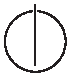
\includegraphics[scale=1.5]{formalities/tum_info_logo}

  \vspace{0.5cm}

\end{center}

%%% End of cover page

% %%% Title page

\thispagestyle{empty}
\begin{center}
  
  \vspace{4cm}
  
  
\includegraphics[scale=2]{formalities/tum_logo_outline}

  \vspace{1cm}

  \LARGE

  \textsc{Technische Universität München}

  \Large

  \textsc{Fakultät für Informatik}

  \vspace{2cm}

  \normalsize
  
  Master's Thesis in Computer Science

  \vspace{2cm}

  \Huge

  Investigation of Stochastic Scheduling Problems

  \vspace{1cm}

  Untersuchung stochastischer Schedulingprobleme

  \vfill

  \normalsize

  \begin{tabular}[h!]{ll}
    Editor & Philipp Müller \\
    Supervisor & Prof. Dr. Ernst W. Mayr \\
    Advisor & Prof. Dr. Ernst W. Mayr \\
    Submission Date & November 13, 2013
  \end{tabular}

  \vspace{0.5cm}

  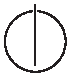
\includegraphics[scale=1.5]{formalities/tum_info_logo}

\end{center}

\newpage

%%% End of title page
% %%% assurements page

\null
\vfill

\section*{Declaration}

\noindent I assure the single handed composition of this master's thesis only supported by declared resources.

\vspace{0.5cm} \noindent Münsing, November 13, 2013

\vspace{1cm} \noindent Philipp Müller

\newpage{}

%%% end of assurements page


% \tableofcontents
% \mainmatter

\chapter{TODO-Lists}
\label{chap:todo}

\section{Strict TODOs}
\label{sec:strict-todos}

\begin{itemize}
\item Titel bei Herrn Mayr anfragen.
\item Show that more processors can not be worse.\done{Ok.}
\item Show that static and dynamic list-scheduling can not be optimal.\done{}
\end{itemize}

\section{Current questions}
\label{chap:current-questions}

\begin{itemize}
\item Gibt es situationen, wo im Optimum auf HLF-level tasks geschedult sind, auf (HLF-1)-level ungeschedulte tasks sind, und auf einem niedrigeren level wieder tasks geschedult sind?\done{Ja! Siehe suboptimal HLF Beispiele}
\item Falls bei einer parallel chain oder einem degenerate intree bereits 2 tasks geschedult sind: Ist es dann optimal, einen HLF-task dazu zu nehmen?
\item Benchmarks: Compare usual LEAF scheduler to SCLEAF and SCLEAF with conjecture that as many topmost tasks as possible shall be sheduled (esp. no. of snapshots is important).\done{Erledigt. Verbesserung von 40\%.}
\item P3: Is it possible, that there are -- at one level of the optimal snapshot DAG -- multiple snapshots containing the same intree, but a different set of scheduled tasks? \remark{Probably not w.l.o.g.}
\item For each snapshot resulting from an optimal schedule, at least one top-most task is scheduled? \remark{Seems so.}
\item If for an intree only non-top tasks are scheduled, you can exchange one of the non-top tasks with a top-tasks and obtain a better run time?\remark{Seems so}
\item ``Topmost singles:'' Are topmost tasks, whose successors have \emph{exactly one} predecessor, always scheduled?\done{No! See chapter ``suboptimal strategies'' (number of topmost tasks).}
\item Are there intrees where we have to schedule topmost tasks of \emph{three different (root-)subtrees? (Root-subtree: Subtree rooted at a direct predecessor of the root.)}\done{Yes. Siehe suboptimal-Kapitel, irgendein non-HLF-optimal-Beispiel.}
\item If a tree $T$ is non-HLF-optimal, can there a be a supertree $S$ of this tree ($T\subseteq S$) such that $S$ is HLF-optimal? \done{Yes, refer to section \ref{sec:properties-optimal-schedules-no-implications}.}
\item Are chain collections optimally scheduled by HLF?\done{Possibly so. Check proof once again.}
\item Let's assume we force the \emph{first step} to be HLF. Is then the best possible solution with exactly this HLF-beginning again HLF?\done{No -- consider the non-HLF examples!}
\end{itemize}

\section{Other TODOs}

\begin{itemize}
\item TikZ export very slow due to \texttt{generate\_tikz\_nodes}.
\item Appendix containing all tree sequences for which optimal schedule is strictly non-HLF.
\end{itemize}

%\renewcommand{\leveltopI}{-15cm + \leveltop}
\renewcommand{\leveltopII}{-15cm + \leveltopI}
\renewcommand{\leveltopIII}{-15cm + \leveltopII}
\renewcommand{\leveltopIIII}{-15cm + \leveltopIII}
\renewcommand{\leveltopIIIII}{-15cm + \leveltopIIII}
\renewcommand{\leveltopIIIIII}{-15cm + \leveltopIIIII}
\renewcommand{\leveltopIIIIIII}{-15cm + \leveltopIIIIII}
\renewcommand{\leveltopIIIIIIII}{-15cm + \leveltopIIIIIII}
\renewcommand{\leveltopIIIIIIIII}{-15cm + \leveltopIIIIIIII}
\renewcommand{\leveltopIIIIIIIIII}{-15cm + \leveltopIIIIIIIII}
\renewcommand{\leveltopIIIIIIIIIII}{-15cm + \leveltopIIIIIIIIII}
\begin{tikzpicture}[scale=.2, anchor=south]
  \begin{scope}[yshift=\leveltopI cm]
    \matrix (line1) [column sep=1cm] {
      \node[draw=black, rectangle split,  rectangle split parts=3] (sn0x104f980){
        \begin{tikzpicture}[scale=.2]
          \node[circle, scale=0.75, fill] (tid0) at (3.75,1.5){};
          \node[circle, scale=0.75, fill] (tid1) at (2.25,3){};
          \node[circle, scale=0.75, fill] (tid3) at (0.75,4.5){};
          \node[circle, scale=0.75, fill] (tid7) at (0.75,6){};
          \draw[](tid3) -- (tid7);
          \node[circle, scale=0.75, fill] (tid4) at (2.25,4.5){};
          \node[circle, scale=0.75, fill] (tid5) at (3.75,4.5){};
          \draw[](tid1) -- (tid3);
          \draw[](tid1) -- (tid4);
          \draw[](tid1) -- (tid5);
          \node[circle, scale=0.75, fill] (tid2) at (6,3){};
          \node[circle, scale=0.75, fill] (tid6) at (6,4.5){};
          \node[circle, scale=0.75, fill] (tid8) at (5.25,6){};
          \node[circle, scale=0.75, fill, red] (tid10) at (5.25,7.5){};
          \draw[](tid8) -- (tid10);
          \node[circle, scale=0.75, fill, red] (tid9) at (6.75,6){};
          \draw[](tid6) -- (tid8);
          \draw[](tid6) -- (tid9);
          \draw[](tid2) -- (tid6);
          \draw[](tid0) -- (tid1);
          \draw[](tid0) -- (tid2);
        \end{tikzpicture}
        \nodepart{two}
        \footnotesize{6.82812}
        \nodepart{three}
        \footnotesize{$50\:25\:25$}
      };
      & 
      \\
    };
  \end{scope}
  \begin{scope}[yshift=\leveltopII cm]
    \matrix (line2) [column sep=1cm] {
      \node[draw=black, rectangle split,  rectangle split parts=3] (sn0x1050190){
        \begin{tikzpicture}[scale=.2]
          \node[circle, scale=0.75, fill] (tid0) at (3,1.5){};
          \node[circle, scale=0.75, fill] (tid1) at (2.25,3){};
          \node[circle, scale=0.75, fill] (tid3) at (0.75,4.5){};
          \node[circle, scale=0.75, fill, red] (tid7) at (0.75,6){};
          \draw[](tid3) -- (tid7);
          \node[circle, scale=0.75, fill] (tid4) at (2.25,4.5){};
          \node[circle, scale=0.75, fill] (tid5) at (3.75,4.5){};
          \draw[](tid1) -- (tid3);
          \draw[](tid1) -- (tid4);
          \draw[](tid1) -- (tid5);
          \node[circle, scale=0.75, fill] (tid2) at (5.25,3){};
          \node[circle, scale=0.75, fill] (tid6) at (5.25,4.5){};
          \node[circle, scale=0.75, fill] (tid8) at (5.25,6){};
          \node[circle, scale=0.75, fill, red] (tid9) at (5.25,7.5){};
          \draw[](tid8) -- (tid9);
          \draw[](tid6) -- (tid8);
          \draw[](tid2) -- (tid6);
          \draw[](tid0) -- (tid1);
          \draw[](tid0) -- (tid2);
        \end{tikzpicture}
        \nodepart{two}
        \footnotesize{6.35938}
        \nodepart{three}
        \footnotesize{$50\:50$}
      };
      & 
      \node[draw=black, rectangle split,  rectangle split parts=3] (sn0x104cb60){
        \begin{tikzpicture}[scale=.2]
          \node[circle, scale=0.75, fill] (tid0) at (3.75,1.5){};
          \node[circle, scale=0.75, fill] (tid1) at (2.25,3){};
          \node[circle, scale=0.75, fill] (tid3) at (0.75,4.5){};
          \node[circle, scale=0.75, fill, red] (tid7) at (0.75,6){};
          \draw[](tid3) -- (tid7);
          \node[circle, scale=0.75, fill] (tid4) at (2.25,4.5){};
          \node[circle, scale=0.75, fill] (tid5) at (3.75,4.5){};
          \draw[](tid1) -- (tid3);
          \draw[](tid1) -- (tid4);
          \draw[](tid1) -- (tid5);
          \node[circle, scale=0.75, fill] (tid2) at (6,3){};
          \node[circle, scale=0.75, fill] (tid6) at (6,4.5){};
          \node[circle, scale=0.75, fill, red] (tid8) at (5.25,6){};
          \node[circle, scale=0.75, fill] (tid9) at (6.75,6){};
          \draw[](tid6) -- (tid8);
          \draw[](tid6) -- (tid9);
          \draw[](tid2) -- (tid6);
          \draw[](tid0) -- (tid1);
          \draw[](tid0) -- (tid2);
        \end{tikzpicture}
        \nodepart{two}
        \footnotesize{6.29688}
        \nodepart{three}
        \footnotesize{$50\:50$}
      };
      & 
      \node[draw=black, rectangle split,  rectangle split parts=3] (sn0x104dd20){
        \begin{tikzpicture}[scale=.2]
          \node[circle, scale=0.75, fill] (tid0) at (3.75,1.5){};
          \node[circle, scale=0.75, fill] (tid1) at (2.25,3){};
          \node[circle, scale=0.75, fill] (tid3) at (0.75,4.5){};
          \node[circle, scale=0.75, fill] (tid7) at (0.75,6){};
          \draw[](tid3) -- (tid7);
          \node[circle, scale=0.75, fill] (tid4) at (2.25,4.5){};
          \node[circle, scale=0.75, fill] (tid5) at (3.75,4.5){};
          \draw[](tid1) -- (tid3);
          \draw[](tid1) -- (tid4);
          \draw[](tid1) -- (tid5);
          \node[circle, scale=0.75, fill] (tid2) at (6,3){};
          \node[circle, scale=0.75, fill] (tid6) at (6,4.5){};
          \node[circle, scale=0.75, fill, red] (tid8) at (5.25,6){};
          \node[circle, scale=0.75, fill, red] (tid9) at (6.75,6){};
          \draw[](tid6) -- (tid8);
          \draw[](tid6) -- (tid9);
          \draw[](tid2) -- (tid6);
          \draw[](tid0) -- (tid1);
          \draw[](tid0) -- (tid2);
        \end{tikzpicture}
        \nodepart{two}
        \footnotesize{6.29688}
        \nodepart{three}
        \footnotesize{$1$}
      };
      & 
      \\
    };
  \end{scope}
  \begin{scope}[yshift=\leveltopIII cm]
    \matrix (line3) [column sep=1cm] {
      \node[draw=black, rectangle split,  rectangle split parts=3] (sn0x10519d0){
        \begin{tikzpicture}[scale=.2]
          \node[circle, scale=0.75, fill] (tid0) at (3,1.5){};
          \node[circle, scale=0.75, fill] (tid1) at (2.25,3){};
          \node[circle, scale=0.75, fill, red] (tid3) at (0.75,4.5){};
          \node[circle, scale=0.75, fill] (tid4) at (2.25,4.5){};
          \node[circle, scale=0.75, fill] (tid5) at (3.75,4.5){};
          \draw[](tid1) -- (tid3);
          \draw[](tid1) -- (tid4);
          \draw[](tid1) -- (tid5);
          \node[circle, scale=0.75, fill] (tid2) at (5.25,3){};
          \node[circle, scale=0.75, fill] (tid6) at (5.25,4.5){};
          \node[circle, scale=0.75, fill] (tid7) at (5.25,6){};
          \node[circle, scale=0.75, fill, red] (tid8) at (5.25,7.5){};
          \draw[](tid7) -- (tid8);
          \draw[](tid6) -- (tid7);
          \draw[](tid2) -- (tid6);
          \draw[](tid0) -- (tid1);
          \draw[](tid0) -- (tid2);
        \end{tikzpicture}
        \nodepart{two}
        \footnotesize{5.92188}
        \nodepart{three}
        \footnotesize{$50\:50$}
      };
      & 
      \node[draw=black, rectangle split,  rectangle split parts=3] (sn0x104fbd0){
        \begin{tikzpicture}[scale=.2]
          \node[circle, scale=0.75, fill] (tid0) at (3,1.5){};
          \node[circle, scale=0.75, fill] (tid1) at (2.25,3){};
          \node[circle, scale=0.75, fill] (tid3) at (0.75,4.5){};
          \node[circle, scale=0.75, fill, red] (tid7) at (0.75,6){};
          \draw[](tid3) -- (tid7);
          \node[circle, scale=0.75, fill] (tid4) at (2.25,4.5){};
          \node[circle, scale=0.75, fill] (tid5) at (3.75,4.5){};
          \draw[](tid1) -- (tid3);
          \draw[](tid1) -- (tid4);
          \draw[](tid1) -- (tid5);
          \node[circle, scale=0.75, fill] (tid2) at (5.25,3){};
          \node[circle, scale=0.75, fill] (tid6) at (5.25,4.5){};
          \node[circle, scale=0.75, fill, red] (tid8) at (5.25,6){};
          \draw[](tid6) -- (tid8);
          \draw[](tid2) -- (tid6);
          \draw[](tid0) -- (tid1);
          \draw[](tid0) -- (tid2);
        \end{tikzpicture}
        \nodepart{two}
        \footnotesize{5.79688}
        \nodepart{three}
        \footnotesize{$50\:33\:17$}
      };
      & 
      \node[draw=black, rectangle split,  rectangle split parts=3] (sn0x105a080){
        \begin{tikzpicture}[scale=.2]
          \node[circle, scale=0.75, fill] (tid0) at (3.75,1.5){};
          \node[circle, scale=0.75, fill] (tid1) at (2.25,3){};
          \node[circle, scale=0.75, fill] (tid3) at (0.75,4.5){};
          \node[circle, scale=0.75, fill] (tid4) at (2.25,4.5){};
          \node[circle, scale=0.75, fill] (tid5) at (3.75,4.5){};
          \draw[](tid1) -- (tid3);
          \draw[](tid1) -- (tid4);
          \draw[](tid1) -- (tid5);
          \node[circle, scale=0.75, fill] (tid2) at (6,3){};
          \node[circle, scale=0.75, fill] (tid6) at (6,4.5){};
          \node[circle, scale=0.75, fill, red] (tid7) at (5.25,6){};
          \node[circle, scale=0.75, fill, red] (tid8) at (6.75,6){};
          \draw[](tid6) -- (tid7);
          \draw[](tid6) -- (tid8);
          \draw[](tid2) -- (tid6);
          \draw[](tid0) -- (tid1);
          \draw[](tid0) -- (tid2);
        \end{tikzpicture}
        \nodepart{two}
        \footnotesize{5.79688}
        \nodepart{three}
        \footnotesize{$1$}
      };
      & 
      \\
    };
  \end{scope}
  \begin{scope}[yshift=\leveltopIIII cm]
    \matrix (line4) [column sep=1cm] {
      \node[draw=black, rectangle split,  rectangle split parts=3] (sn0x1052250){
        \begin{tikzpicture}[scale=.2]
          \node[circle, scale=0.75, fill] (tid0) at (2.25,1.5){};
          \node[circle, scale=0.75, fill] (tid1) at (0.75,3){};
          \node[circle, scale=0.75, fill] (tid3) at (0.75,4.5){};
          \node[circle, scale=0.75, fill] (tid6) at (0.75,6){};
          \node[circle, scale=0.75, fill, red] (tid7) at (0.75,7.5){};
          \draw[](tid6) -- (tid7);
          \draw[](tid3) -- (tid6);
          \draw[](tid1) -- (tid3);
          \node[circle, scale=0.75, fill] (tid2) at (3,3){};
          \node[circle, scale=0.75, fill, red] (tid4) at (2.25,4.5){};
          \node[circle, scale=0.75, fill] (tid5) at (3.75,4.5){};
          \draw[](tid2) -- (tid4);
          \draw[](tid2) -- (tid5);
          \draw[](tid0) -- (tid1);
          \draw[](tid0) -- (tid2);
        \end{tikzpicture}
        \nodepart{two}
        \footnotesize{5.54688}
        \nodepart{three}
        \footnotesize{$50\:50$}
      };
      & 
      \node[draw=black, rectangle split,  rectangle split parts=3] (sn0x1052960){
        \begin{tikzpicture}[scale=.2]
          \node[circle, scale=0.75, fill] (tid0) at (3,1.5){};
          \node[circle, scale=0.75, fill] (tid1) at (2.25,3){};
          \node[circle, scale=0.75, fill, red] (tid3) at (0.75,4.5){};
          \node[circle, scale=0.75, fill] (tid4) at (2.25,4.5){};
          \node[circle, scale=0.75, fill] (tid5) at (3.75,4.5){};
          \draw[](tid1) -- (tid3);
          \draw[](tid1) -- (tid4);
          \draw[](tid1) -- (tid5);
          \node[circle, scale=0.75, fill] (tid2) at (5.25,3){};
          \node[circle, scale=0.75, fill] (tid6) at (5.25,4.5){};
          \node[circle, scale=0.75, fill, red] (tid7) at (5.25,6){};
          \draw[](tid6) -- (tid7);
          \draw[](tid2) -- (tid6);
          \draw[](tid0) -- (tid1);
          \draw[](tid0) -- (tid2);
        \end{tikzpicture}
        \nodepart{two}
        \footnotesize{5.29688}
        \nodepart{three}
        \footnotesize{$50\:33\:17$}
      };
      & 
      \node[draw=black, rectangle split,  rectangle split parts=3] (sn0x10581e0){
        \begin{tikzpicture}[scale=.2]
          \node[circle, scale=0.75, fill] (tid0) at (3,1.5){};
          \node[circle, scale=0.75, fill] (tid1) at (2.25,3){};
          \node[circle, scale=0.75, fill] (tid3) at (0.75,4.5){};
          \node[circle, scale=0.75, fill, red] (tid7) at (0.75,6){};
          \draw[](tid3) -- (tid7);
          \node[circle, scale=0.75, fill, red] (tid4) at (2.25,4.5){};
          \node[circle, scale=0.75, fill] (tid5) at (3.75,4.5){};
          \draw[](tid1) -- (tid3);
          \draw[](tid1) -- (tid4);
          \draw[](tid1) -- (tid5);
          \node[circle, scale=0.75, fill] (tid2) at (5.25,3){};
          \node[circle, scale=0.75, fill] (tid6) at (5.25,4.5){};
          \draw[](tid2) -- (tid6);
          \draw[](tid0) -- (tid1);
          \draw[](tid0) -- (tid2);
        \end{tikzpicture}
        \nodepart{two}
        \footnotesize{5.29688}
        \nodepart{three}
        \footnotesize{$33\:17\:25\:25$}
      };
      & 
      \node[draw=black, rectangle split,  rectangle split parts=3] (sn0x1058550){
        \begin{tikzpicture}[scale=.2]
          \node[circle, scale=0.75, fill] (tid0) at (3,1.5){};
          \node[circle, scale=0.75, fill] (tid1) at (2.25,3){};
          \node[circle, scale=0.75, fill] (tid3) at (0.75,4.5){};
          \node[circle, scale=0.75, fill, red] (tid7) at (0.75,6){};
          \draw[](tid3) -- (tid7);
          \node[circle, scale=0.75, fill] (tid4) at (2.25,4.5){};
          \node[circle, scale=0.75, fill] (tid5) at (3.75,4.5){};
          \draw[](tid1) -- (tid3);
          \draw[](tid1) -- (tid4);
          \draw[](tid1) -- (tid5);
          \node[circle, scale=0.75, fill] (tid2) at (5.25,3){};
          \node[circle, scale=0.75, fill, red] (tid6) at (5.25,4.5){};
          \draw[](tid2) -- (tid6);
          \draw[](tid0) -- (tid1);
          \draw[](tid0) -- (tid2);
        \end{tikzpicture}
        \nodepart{two}
        \footnotesize{5.29688}
        \nodepart{three}
        \footnotesize{$50\:50$}
      };
      & 
      \\
    };
  \end{scope}
  \begin{scope}[yshift=\leveltopIIIII cm]
    \matrix (line5) [column sep=1cm] {
      \node[draw=black, rectangle split,  rectangle split parts=3] (sn0x10525f0){
        \begin{tikzpicture}[scale=.2]
          \node[circle, scale=0.75, fill] (tid0) at (1.5,1.5){};
          \node[circle, scale=0.75, fill] (tid1) at (0.75,3){};
          \node[circle, scale=0.75, fill] (tid3) at (0.75,4.5){};
          \node[circle, scale=0.75, fill] (tid5) at (0.75,6){};
          \node[circle, scale=0.75, fill, red] (tid6) at (0.75,7.5){};
          \draw[](tid5) -- (tid6);
          \draw[](tid3) -- (tid5);
          \draw[](tid1) -- (tid3);
          \node[circle, scale=0.75, fill] (tid2) at (2.25,3){};
          \node[circle, scale=0.75, fill, red] (tid4) at (2.25,4.5){};
          \draw[](tid2) -- (tid4);
          \draw[](tid0) -- (tid1);
          \draw[](tid0) -- (tid2);
        \end{tikzpicture}
        \nodepart{two}
        \footnotesize{5.25}
        \nodepart{three}
        \footnotesize{$50\:50$}
      };
      & 
      \node[draw=black, rectangle split,  rectangle split parts=3] (sn0x1053850){
        \begin{tikzpicture}[scale=.2]
          \node[circle, scale=0.75, fill] (tid0) at (2.25,1.5){};
          \node[circle, scale=0.75, fill] (tid1) at (1.5,3){};
          \node[circle, scale=0.75, fill, red] (tid3) at (0.75,4.5){};
          \node[circle, scale=0.75, fill] (tid4) at (2.25,4.5){};
          \draw[](tid1) -- (tid3);
          \draw[](tid1) -- (tid4);
          \node[circle, scale=0.75, fill] (tid2) at (3.75,3){};
          \node[circle, scale=0.75, fill] (tid5) at (3.75,4.5){};
          \node[circle, scale=0.75, fill, red] (tid6) at (3.75,6){};
          \draw[](tid5) -- (tid6);
          \draw[](tid2) -- (tid5);
          \draw[](tid0) -- (tid1);
          \draw[](tid0) -- (tid2);
        \end{tikzpicture}
        \nodepart{two}
        \footnotesize{4.84375}
        \nodepart{three}
        \footnotesize{$50\:25\:25$}
      };
      & 
      \node[draw=black, rectangle split,  rectangle split parts=3] (sn0x1056b00){
        \begin{tikzpicture}[scale=.2]
          \node[circle, scale=0.75, fill] (tid0) at (3,1.5){};
          \node[circle, scale=0.75, fill] (tid1) at (2.25,3){};
          \node[circle, scale=0.75, fill, red] (tid3) at (0.75,4.5){};
          \node[circle, scale=0.75, fill, red] (tid4) at (2.25,4.5){};
          \node[circle, scale=0.75, fill] (tid5) at (3.75,4.5){};
          \draw[](tid1) -- (tid3);
          \draw[](tid1) -- (tid4);
          \draw[](tid1) -- (tid5);
          \node[circle, scale=0.75, fill] (tid2) at (5.25,3){};
          \node[circle, scale=0.75, fill] (tid6) at (5.25,4.5){};
          \draw[](tid2) -- (tid6);
          \draw[](tid0) -- (tid1);
          \draw[](tid0) -- (tid2);
        \end{tikzpicture}
        \nodepart{two}
        \footnotesize{4.75}
        \nodepart{three}
        \footnotesize{$50\:50$}
      };
      & 
      \node[draw=black, rectangle split,  rectangle split parts=3] (sn0x1056fb0){
        \begin{tikzpicture}[scale=.2]
          \node[circle, scale=0.75, fill] (tid0) at (3,1.5){};
          \node[circle, scale=0.75, fill] (tid1) at (2.25,3){};
          \node[circle, scale=0.75, fill, red] (tid3) at (0.75,4.5){};
          \node[circle, scale=0.75, fill] (tid4) at (2.25,4.5){};
          \node[circle, scale=0.75, fill] (tid5) at (3.75,4.5){};
          \draw[](tid1) -- (tid3);
          \draw[](tid1) -- (tid4);
          \draw[](tid1) -- (tid5);
          \node[circle, scale=0.75, fill] (tid2) at (5.25,3){};
          \node[circle, scale=0.75, fill, red] (tid6) at (5.25,4.5){};
          \draw[](tid2) -- (tid6);
          \draw[](tid0) -- (tid1);
          \draw[](tid0) -- (tid2);
        \end{tikzpicture}
        \nodepart{two}
        \footnotesize{4.75}
        \nodepart{three}
        \footnotesize{$50\:50$}
      };
      & 
      \node[draw=black, rectangle split,  rectangle split parts=3] (sn0x1058f50){
        \begin{tikzpicture}[scale=.2]
          \node[circle, scale=0.75, fill] (tid0) at (2.25,1.5){};
          \node[circle, scale=0.75, fill] (tid1) at (1.5,3){};
          \node[circle, scale=0.75, fill] (tid3) at (0.75,4.5){};
          \node[circle, scale=0.75, fill, red] (tid6) at (0.75,6){};
          \draw[](tid3) -- (tid6);
          \node[circle, scale=0.75, fill, red] (tid4) at (2.25,4.5){};
          \draw[](tid1) -- (tid3);
          \draw[](tid1) -- (tid4);
          \node[circle, scale=0.75, fill] (tid2) at (3.75,3){};
          \node[circle, scale=0.75, fill] (tid5) at (3.75,4.5){};
          \draw[](tid2) -- (tid5);
          \draw[](tid0) -- (tid1);
          \draw[](tid0) -- (tid2);
        \end{tikzpicture}
        \nodepart{two}
        \footnotesize{4.84375}
        \nodepart{three}
        \footnotesize{$50\:25\:25$}
      };
      & 
      \node[draw=black, rectangle split,  rectangle split parts=3] (sn0x1058a50){
        \begin{tikzpicture}[scale=.2]
          \node[circle, scale=0.75, fill] (tid0) at (2.25,1.5){};
          \node[circle, scale=0.75, fill] (tid1) at (1.5,3){};
          \node[circle, scale=0.75, fill] (tid3) at (0.75,4.5){};
          \node[circle, scale=0.75, fill, red] (tid6) at (0.75,6){};
          \draw[](tid3) -- (tid6);
          \node[circle, scale=0.75, fill] (tid4) at (2.25,4.5){};
          \draw[](tid1) -- (tid3);
          \draw[](tid1) -- (tid4);
          \node[circle, scale=0.75, fill] (tid2) at (3.75,3){};
          \node[circle, scale=0.75, fill, red] (tid5) at (3.75,4.5){};
          \draw[](tid2) -- (tid5);
          \draw[](tid0) -- (tid1);
          \draw[](tid0) -- (tid2);
        \end{tikzpicture}
        \nodepart{two}
        \footnotesize{4.84375}
        \nodepart{three}
        \footnotesize{$50\:50$}
      };
      & 
      \node[draw=black, rectangle split,  rectangle split parts=3] (sn0x10597a0){
        \begin{tikzpicture}[scale=.2]
          \node[circle, scale=0.75, fill] (tid0) at (3,1.5){};
          \node[circle, scale=0.75, fill] (tid1) at (2.25,3){};
          \node[circle, scale=0.75, fill] (tid3) at (0.75,4.5){};
          \node[circle, scale=0.75, fill, red] (tid6) at (0.75,6){};
          \draw[](tid3) -- (tid6);
          \node[circle, scale=0.75, fill, red] (tid4) at (2.25,4.5){};
          \node[circle, scale=0.75, fill] (tid5) at (3.75,4.5){};
          \draw[](tid1) -- (tid3);
          \draw[](tid1) -- (tid4);
          \draw[](tid1) -- (tid5);
          \node[circle, scale=0.75, fill] (tid2) at (5.25,3){};
          \draw[](tid0) -- (tid1);
          \draw[](tid0) -- (tid2);
        \end{tikzpicture}
        \nodepart{two}
        \footnotesize{4.84375}
        \nodepart{three}
        \footnotesize{$50\:50$}
      };
      & 
      \\
    };
  \end{scope}
  \begin{scope}[yshift=\leveltopIIIIII cm]
    \matrix (line6) [column sep=1cm] {
      \node[draw=black, rectangle split,  rectangle split parts=3] (sn0x1053920){
        \begin{tikzpicture}[scale=.2]
          \node[circle, scale=0.75, fill] (tid0) at (1.5,1.5){};
          \node[circle, scale=0.75, fill] (tid1) at (0.75,3){};
          \node[circle, scale=0.75, fill] (tid3) at (0.75,4.5){};
          \node[circle, scale=0.75, fill] (tid4) at (0.75,6){};
          \node[circle, scale=0.75, fill, red] (tid5) at (0.75,7.5){};
          \draw[](tid4) -- (tid5);
          \draw[](tid3) -- (tid4);
          \draw[](tid1) -- (tid3);
          \node[circle, scale=0.75, fill, red] (tid2) at (2.25,3){};
          \draw[](tid0) -- (tid1);
          \draw[](tid0) -- (tid2);
        \end{tikzpicture}
        \nodepart{two}
        \footnotesize{5.0625}
        \nodepart{three}
        \footnotesize{$50\:50$}
      };
      & 
      \node[draw=black, rectangle split,  rectangle split parts=3] (sn0x1053bc0){
        \begin{tikzpicture}[scale=.2]
          \node[circle, scale=0.75, fill] (tid0) at (1.5,1.5){};
          \node[circle, scale=0.75, fill] (tid1) at (0.75,3){};
          \node[circle, scale=0.75, fill] (tid3) at (0.75,4.5){};
          \node[circle, scale=0.75, fill, red] (tid5) at (0.75,6){};
          \draw[](tid3) -- (tid5);
          \draw[](tid1) -- (tid3);
          \node[circle, scale=0.75, fill] (tid2) at (2.25,3){};
          \node[circle, scale=0.75, fill, red] (tid4) at (2.25,4.5){};
          \draw[](tid2) -- (tid4);
          \draw[](tid0) -- (tid1);
          \draw[](tid0) -- (tid2);
        \end{tikzpicture}
        \nodepart{two}
        \footnotesize{4.4375}
        \nodepart{three}
        \footnotesize{$50\:50$}
      };
      & 
      \node[draw=black, rectangle split,  rectangle split parts=3] (sn0x1056090){
        \begin{tikzpicture}[scale=.2]
          \node[circle, scale=0.75, fill] (tid0) at (2.25,1.5){};
          \node[circle, scale=0.75, fill] (tid1) at (1.5,3){};
          \node[circle, scale=0.75, fill, red] (tid3) at (0.75,4.5){};
          \node[circle, scale=0.75, fill, red] (tid4) at (2.25,4.5){};
          \draw[](tid1) -- (tid3);
          \draw[](tid1) -- (tid4);
          \node[circle, scale=0.75, fill] (tid2) at (3.75,3){};
          \node[circle, scale=0.75, fill] (tid5) at (3.75,4.5){};
          \draw[](tid2) -- (tid5);
          \draw[](tid0) -- (tid1);
          \draw[](tid0) -- (tid2);
        \end{tikzpicture}
        \nodepart{two}
        \footnotesize{4.25}
        \nodepart{three}
        \footnotesize{$1$}
      };
      & 
      \node[draw=black, rectangle split,  rectangle split parts=3] (sn0x1056160){
        \begin{tikzpicture}[scale=.2]
          \node[circle, scale=0.75, fill] (tid0) at (2.25,1.5){};
          \node[circle, scale=0.75, fill] (tid1) at (1.5,3){};
          \node[circle, scale=0.75, fill, red] (tid3) at (0.75,4.5){};
          \node[circle, scale=0.75, fill] (tid4) at (2.25,4.5){};
          \draw[](tid1) -- (tid3);
          \draw[](tid1) -- (tid4);
          \node[circle, scale=0.75, fill] (tid2) at (3.75,3){};
          \node[circle, scale=0.75, fill, red] (tid5) at (3.75,4.5){};
          \draw[](tid2) -- (tid5);
          \draw[](tid0) -- (tid1);
          \draw[](tid0) -- (tid2);
        \end{tikzpicture}
        \nodepart{two}
        \footnotesize{4.25}
        \nodepart{three}
        \footnotesize{$50\:50$}
      };
      & 
      \node[draw=black, rectangle split,  rectangle split parts=3] (sn0x1057630){
        \begin{tikzpicture}[scale=.2]
          \node[circle, scale=0.75, fill] (tid0) at (3,1.5){};
          \node[circle, scale=0.75, fill] (tid1) at (2.25,3){};
          \node[circle, scale=0.75, fill, red] (tid3) at (0.75,4.5){};
          \node[circle, scale=0.75, fill, red] (tid4) at (2.25,4.5){};
          \node[circle, scale=0.75, fill] (tid5) at (3.75,4.5){};
          \draw[](tid1) -- (tid3);
          \draw[](tid1) -- (tid4);
          \draw[](tid1) -- (tid5);
          \node[circle, scale=0.75, fill] (tid2) at (5.25,3){};
          \draw[](tid0) -- (tid1);
          \draw[](tid0) -- (tid2);
        \end{tikzpicture}
        \nodepart{two}
        \footnotesize{4.25}
        \nodepart{three}
        \footnotesize{$1$}
      };
      & 
      \node[draw=black, rectangle split,  rectangle split parts=3] (sn0x1058b20){
        \begin{tikzpicture}[scale=.2]
          \node[circle, scale=0.75, fill] (tid0) at (2.25,1.5){};
          \node[circle, scale=0.75, fill] (tid1) at (1.5,3){};
          \node[circle, scale=0.75, fill] (tid3) at (0.75,4.5){};
          \node[circle, scale=0.75, fill, red] (tid5) at (0.75,6){};
          \draw[](tid3) -- (tid5);
          \node[circle, scale=0.75, fill, red] (tid4) at (2.25,4.5){};
          \draw[](tid1) -- (tid3);
          \draw[](tid1) -- (tid4);
          \node[circle, scale=0.75, fill] (tid2) at (3.75,3){};
          \draw[](tid0) -- (tid1);
          \draw[](tid0) -- (tid2);
        \end{tikzpicture}
        \nodepart{two}
        \footnotesize{4.4375}
        \nodepart{three}
        \footnotesize{$50\:50$}
      };
      & 
      \\
    };
  \end{scope}
  \begin{scope}[yshift=\leveltopIIIIIII cm]
    \matrix (line7) [column sep=1cm] {
      \node[draw=black, rectangle split,  rectangle split parts=3] (sn0x10540d0){
        \begin{tikzpicture}[scale=.2]
          \node[circle, scale=0.75, fill] (tid0) at (0.75,1.5){};
          \node[circle, scale=0.75, fill] (tid1) at (0.75,3){};
          \node[circle, scale=0.75, fill] (tid2) at (0.75,4.5){};
          \node[circle, scale=0.75, fill] (tid3) at (0.75,6){};
          \node[circle, scale=0.75, fill, red] (tid4) at (0.75,7.5){};
          \draw[](tid3) -- (tid4);
          \draw[](tid2) -- (tid3);
          \draw[](tid1) -- (tid2);
          \draw[](tid0) -- (tid1);
        \end{tikzpicture}
        \nodepart{two}
        \footnotesize{5}
        \nodepart{three}
        \footnotesize{$1$}
      };
      & 
      \node[draw=black, rectangle split,  rectangle split parts=3] (sn0x1054480){
        \begin{tikzpicture}[scale=.2]
          \node[circle, scale=0.75, fill] (tid0) at (1.5,1.5){};
          \node[circle, scale=0.75, fill] (tid1) at (0.75,3){};
          \node[circle, scale=0.75, fill] (tid3) at (0.75,4.5){};
          \node[circle, scale=0.75, fill, red] (tid4) at (0.75,6){};
          \draw[](tid3) -- (tid4);
          \draw[](tid1) -- (tid3);
          \node[circle, scale=0.75, fill, red] (tid2) at (2.25,3){};
          \draw[](tid0) -- (tid1);
          \draw[](tid0) -- (tid2);
        \end{tikzpicture}
        \nodepart{two}
        \footnotesize{4.125}
        \nodepart{three}
        \footnotesize{$50\:50$}
      };
      & 
      \node[draw=black, rectangle split,  rectangle split parts=3] (sn0x1055dd0){
        \begin{tikzpicture}[scale=.2]
          \node[circle, scale=0.75, fill] (tid0) at (1.5,1.5){};
          \node[circle, scale=0.75, fill] (tid1) at (0.75,3){};
          \node[circle, scale=0.75, fill, red] (tid3) at (0.75,4.5){};
          \draw[](tid1) -- (tid3);
          \node[circle, scale=0.75, fill] (tid2) at (2.25,3){};
          \node[circle, scale=0.75, fill, red] (tid4) at (2.25,4.5){};
          \draw[](tid2) -- (tid4);
          \draw[](tid0) -- (tid1);
          \draw[](tid0) -- (tid2);
        \end{tikzpicture}
        \nodepart{two}
        \footnotesize{3.75}
        \nodepart{three}
        \footnotesize{$1$}
      };
      & 
      \node[draw=black, rectangle split,  rectangle split parts=3] (sn0x10568c0){
        \begin{tikzpicture}[scale=.2]
          \node[circle, scale=0.75, fill] (tid0) at (2.25,1.5){};
          \node[circle, scale=0.75, fill] (tid1) at (1.5,3){};
          \node[circle, scale=0.75, fill, red] (tid3) at (0.75,4.5){};
          \node[circle, scale=0.75, fill, red] (tid4) at (2.25,4.5){};
          \draw[](tid1) -- (tid3);
          \draw[](tid1) -- (tid4);
          \node[circle, scale=0.75, fill] (tid2) at (3.75,3){};
          \draw[](tid0) -- (tid1);
          \draw[](tid0) -- (tid2);
        \end{tikzpicture}
        \nodepart{two}
        \footnotesize{3.75}
        \nodepart{three}
        \footnotesize{$1$}
      };
      & 
      \\
    };
  \end{scope}
  \begin{scope}[yshift=\leveltopIIIIIIII cm]
    \matrix (line8) [column sep=1cm] {
      \node[draw=black, rectangle split,  rectangle split parts=3] (sn0x1054550){
        \begin{tikzpicture}[scale=.2]
          \node[circle, scale=0.75, fill] (tid0) at (0.75,1.5){};
          \node[circle, scale=0.75, fill] (tid1) at (0.75,3){};
          \node[circle, scale=0.75, fill] (tid2) at (0.75,4.5){};
          \node[circle, scale=0.75, fill, red] (tid3) at (0.75,6){};
          \draw[](tid2) -- (tid3);
          \draw[](tid1) -- (tid2);
          \draw[](tid0) -- (tid1);
        \end{tikzpicture}
        \nodepart{two}
        \footnotesize{4}
        \nodepart{three}
        \footnotesize{$1$}
      };
      & 
      \node[draw=black, rectangle split,  rectangle split parts=3] (sn0x1055270){
        \begin{tikzpicture}[scale=.2]
          \node[circle, scale=0.75, fill] (tid0) at (1.5,1.5){};
          \node[circle, scale=0.75, fill] (tid1) at (0.75,3){};
          \node[circle, scale=0.75, fill, red] (tid3) at (0.75,4.5){};
          \draw[](tid1) -- (tid3);
          \node[circle, scale=0.75, fill, red] (tid2) at (2.25,3){};
          \draw[](tid0) -- (tid1);
          \draw[](tid0) -- (tid2);
        \end{tikzpicture}
        \nodepart{two}
        \footnotesize{3.25}
        \nodepart{three}
        \footnotesize{$50\:50$}
      };
      & 
      \\
    };
  \end{scope}
  \begin{scope}[yshift=\leveltopIIIIIIIII cm]
    \matrix (line9) [column sep=1cm] {
      \node[draw=black, rectangle split,  rectangle split parts=3] (sn0x1054a50){
        \begin{tikzpicture}[scale=.2]
          \node[circle, scale=0.75, fill] (tid0) at (0.75,1.5){};
          \node[circle, scale=0.75, fill] (tid1) at (0.75,3){};
          \node[circle, scale=0.75, fill, red] (tid2) at (0.75,4.5){};
          \draw[](tid1) -- (tid2);
          \draw[](tid0) -- (tid1);
        \end{tikzpicture}
        \nodepart{two}
        \footnotesize{3}
        \nodepart{three}
        \footnotesize{$1$}
      };
      & 
      \node[draw=black, rectangle split,  rectangle split parts=3] (sn0x1054cb0){
        \begin{tikzpicture}[scale=.2]
          \node[circle, scale=0.75, fill] (tid0) at (1.5,1.5){};
          \node[circle, scale=0.75, fill, red] (tid1) at (0.75,3){};
          \node[circle, scale=0.75, fill, red] (tid2) at (2.25,3){};
          \draw[](tid0) -- (tid1);
          \draw[](tid0) -- (tid2);
        \end{tikzpicture}
        \nodepart{two}
        \footnotesize{2.5}
        \nodepart{three}
        \footnotesize{$1$}
      };
      & 
      \\
    };
  \end{scope}
  \begin{scope}[yshift=\leveltopIIIIIIIIII cm]
    \matrix (line10) [column sep=1cm] {
      \node[draw=black, rectangle split,  rectangle split parts=3] (sn0x1054b20){
        \begin{tikzpicture}[scale=.2]
          \node[circle, scale=0.75, fill] (tid0) at (0.75,1.5){};
          \node[circle, scale=0.75, fill, red] (tid1) at (0.75,3){};
          \draw[](tid0) -- (tid1);
        \end{tikzpicture}
        \nodepart{two}
        \footnotesize{2}
        \nodepart{three}
        \footnotesize{$1$}
      };
      & 
      \\
    };
  \end{scope}
  \begin{scope}[yshift=\leveltopIIIIIIIIIII cm]
    \matrix (line11) [column sep=1cm] {
      \node[draw=black, rectangle split,  rectangle split parts=3] (sn0x10547e0){
        \begin{tikzpicture}[scale=.2]
          \node[circle, scale=0.75, fill, red] (tid0) at (0.75,1.5){};
        \end{tikzpicture}
        \nodepart{two}
        \footnotesize{1}
        \nodepart{three}
        \footnotesize{$$}
      };
      & 
      \\
    };
  \end{scope}
  \begin{scope}[yshift=\leveltopIIIIIIIIIIII cm]
    \matrix (line12) [column sep=1cm] {
      \\
    };
  \end{scope}
  \draw (sn0x104f980.south) -- (sn0x1050190.north);
  \draw (sn0x104f980.south) -- (sn0x104cb60.north);
  \draw (sn0x104f980.south) -- (sn0x104dd20.north);
  \draw (sn0x1050190.south) -- (sn0x10519d0.north);
  \draw (sn0x1050190.south) -- (sn0x104fbd0.north);
  \draw (sn0x104cb60.south) -- (sn0x105a080.north);
  \draw (sn0x104cb60.south) -- (sn0x104fbd0.north);
  \draw (sn0x104dd20.south) -- (sn0x104fbd0.north);
  \draw (sn0x10519d0.south) -- (sn0x1052250.north);
  \draw (sn0x10519d0.south) -- (sn0x1052960.north);
  \draw (sn0x104fbd0.south) -- (sn0x1052960.north);
  \draw (sn0x104fbd0.south) -- (sn0x10581e0.north);
  \draw (sn0x104fbd0.south) -- (sn0x1058550.north);
  \draw (sn0x105a080.south) -- (sn0x1052960.north);
  \draw (sn0x1052250.south) -- (sn0x10525f0.north);
  \draw (sn0x1052250.south) -- (sn0x1053850.north);
  \draw (sn0x1052960.south) -- (sn0x1053850.north);
  \draw (sn0x1052960.south) -- (sn0x1056b00.north);
  \draw (sn0x1052960.south) -- (sn0x1056fb0.north);
  \draw (sn0x10581e0.south) -- (sn0x1058f50.north);
  \draw (sn0x10581e0.south) -- (sn0x1058a50.north);
  \draw (sn0x10581e0.south) -- (sn0x1056b00.north);
  \draw (sn0x10581e0.south) -- (sn0x1056fb0.north);
  \draw (sn0x1058550.south) -- (sn0x10597a0.north);
  \draw (sn0x1058550.south) -- (sn0x1056fb0.north);
  \draw (sn0x10525f0.south) -- (sn0x1053920.north);
  \draw (sn0x10525f0.south) -- (sn0x1053bc0.north);
  \draw (sn0x1053850.south) -- (sn0x1053bc0.north);
  \draw (sn0x1053850.south) -- (sn0x1056090.north);
  \draw (sn0x1053850.south) -- (sn0x1056160.north);
  \draw (sn0x1056b00.south) -- (sn0x1056090.north);
  \draw (sn0x1056b00.south) -- (sn0x1056160.north);
  \draw (sn0x1056fb0.south) -- (sn0x1056160.north);
  \draw (sn0x1056fb0.south) -- (sn0x1057630.north);
  \draw (sn0x1058f50.south) -- (sn0x1053bc0.north);
  \draw (sn0x1058f50.south) -- (sn0x1056090.north);
  \draw (sn0x1058f50.south) -- (sn0x1056160.north);
  \draw (sn0x1058a50.south) -- (sn0x1058b20.north);
  \draw (sn0x1058a50.south) -- (sn0x1056160.north);
  \draw (sn0x10597a0.south) -- (sn0x1058b20.north);
  \draw (sn0x10597a0.south) -- (sn0x1057630.north);
  \draw (sn0x1053920.south) -- (sn0x10540d0.north);
  \draw (sn0x1053920.south) -- (sn0x1054480.north);
  \draw (sn0x1053bc0.south) -- (sn0x1054480.north);
  \draw (sn0x1053bc0.south) -- (sn0x1055dd0.north);
  \draw (sn0x1056090.south) -- (sn0x1055dd0.north);
  \draw (sn0x1056160.south) -- (sn0x1055dd0.north);
  \draw (sn0x1056160.south) -- (sn0x10568c0.north);
  \draw (sn0x1057630.south) -- (sn0x10568c0.north);
  \draw (sn0x1058b20.south) -- (sn0x1054480.north);
  \draw (sn0x1058b20.south) -- (sn0x10568c0.north);
  \draw (sn0x10540d0.south) -- (sn0x1054550.north);
  \draw (sn0x1054480.south) -- (sn0x1054550.north);
  \draw (sn0x1054480.south) -- (sn0x1055270.north);
  \draw (sn0x1055dd0.south) -- (sn0x1055270.north);
  \draw (sn0x10568c0.south) -- (sn0x1055270.north);
  \draw (sn0x1054550.south) -- (sn0x1054a50.north);
  \draw (sn0x1055270.south) -- (sn0x1054a50.north);
  \draw (sn0x1055270.south) -- (sn0x1054cb0.north);
  \draw (sn0x1054a50.south) -- (sn0x1054b20.north);
  \draw (sn0x1054cb0.south) -- (sn0x1054b20.north);
  \draw (sn0x1054b20.south) -- (sn0x10547e0.north);

  \newcommand{\nd}[4]{
    \node[draw=black, rectangle split, rectangle split parts=3] (n#1#2) {
      $#1/#2$
      \nodepart{two}
      #3
      \nodepart{three}
      #4
    };
  }

  \begin{scope}[yshift=\leveltopI, xshift=70cm, rectangle, draw=black,anchor=south]
    \matrix (test) [column sep=1cm] {
      \nd{5}{6}{6.82812}{50 50};
      \\
    };
  \end{scope}

  \begin{scope}[yshift=\leveltopII, xshift=70cm, rectangle, draw=black,anchor=south]
    \matrix (test) [column sep=1cm] {
      \nd{5}{5}{6.35938}{50 50};
      &
      \nd{4}{6}{6.29688}{1};
      \\
      };
    \end{scope}

    \begin{scope}[yshift=\leveltopIII, xshift=70cm, rectangle, draw=black,anchor=south]
      \matrix (test) [column sep=1cm] {
        \nd{5}{4}{5.92188}{50 50};
        &
        \nd{4}{5}{5.79688}{1};
        \\
      };
    \end{scope}

    \begin{scope}[yshift=\leveltopIIII, xshift=70cm, rectangle, draw=black,anchor=south]
      \matrix (test) [column sep=1cm] {
        \nd{5}{3}{5.54688}{50 50};
        &
        \nd{4}{4}{5.29688}{50 50};
        \\
      };
    \end{scope}

    \begin{scope}[yshift=\leveltopIIIII, xshift=70cm, rectangle, draw=black,anchor=south]
      \matrix (test) [column sep=1cm] {
        \nd{5}{2}{5.25}{50 50};
        &
        \nd{4}{3}{4.84375}{50 50};
        &
        \nd{3}{4}{5.29688}{1};
        \\
      };
    \end{scope}

    \begin{scope}[yshift=\leveltopIIIIII, xshift=70cm, rectangle, draw=black,anchor=south]
      \matrix (test) [column sep=1cm] {
        \nd{5}{1}{5.0625}{50 50};
        &
        \nd{4}{2}{4.4375}{50 50};
        &
        \nd{3}{3}{5.75}{1};
        \\
      };
    \end{scope}

    \begin{scope}[yshift=\leveltopIIIIIII, xshift=70cm, rectangle, draw=black,anchor=south]
      \matrix (test) [column sep=1cm] {
        \nd{5}{0}{5}{50 50};
        &
        \nd{4}{1}{4.125}{50 50};
        &
        \nd{3}{2}{5.25}{1};
        \\
      };
    \end{scope}
    
    \begin{scope}[yshift=\leveltopIIIIIIII, xshift=70cm, rectangle, draw=black,anchor=south]
      \matrix (test) [column sep=1cm] {
        \nd{4}{0}{4}{1};
        &
        \nd{3}{1}{3.25}{50 50};
        \\
      };
    \end{scope}

    \begin{scope}[yshift=\leveltopIIIIIIIII, xshift=70cm, rectangle, draw=black,anchor=south]
      \matrix (test) [column sep=1cm] {
        \nd{3}{0}{3}{1};
        &
        \nd{2}{1}{2.5}{1};
        \\
      };
    \end{scope}

    \begin{scope}[yshift=\leveltopIIIIIIIIII, xshift=70cm, rectangle, draw=black,anchor=south]
      \matrix (test) [column sep=1cm] {
        \nd{2}{0}{2}{1};
        \\
      };
    \end{scope}
    
    \begin{scope}[yshift=\leveltopIIIIIIIIIII, xshift=70cm, rectangle, draw=black,anchor=south]
      \matrix (test) [column sep=1cm] {
        \nd{1}{0}{1}{1};
        \\
      };
    \end{scope}

    \draw (n56.south) -- (n55.north);
    \draw (n56.south) -- (n46.north);
    \draw (n55.south) -- (n54.north);
    \draw (n55.south) -- (n45.north);
    \draw (n46.south) -- (n45.north);
    \draw (n54.south) -- (n53.north);
    \draw (n54.south) -- (n44.north);
    \draw (n45.south) -- (n44.north);
    \draw (n53.south) -- (n52.north);
    \draw (n53.south) -- (n43.north);
    \draw (n44.south) -- (n43.north);
    \draw (n44.south) -- (n34.north);
    \draw (n52.south) -- (n51.north);
    \draw (n52.south) -- (n42.north);
    \draw (n43.south) -- (n42.north);
    \draw (n43.south) -- (n33.north);
    \draw (n34.south) -- (n33.north);
    \draw (n51.south) -- (n50.north);
    \draw (n51.south) -- (n41.north);
    \draw (n42.south) -- (n41.north);
    \draw (n42.south) -- (n32.north);
    \draw (n33.south) -- (n32.north);
    \draw (n32.south) -- (n31.north);
    \draw (n50.south) -- (n40.north);
    \draw (n41.south) -- (n40.north);
    \draw (n41.south) -- (n31.north);
    \draw (n40.south) -- (n30.north);
    \draw (n31.south) -- (n30.north);
    \draw (n31.south) -- (n21.north);
    \draw (n30.south) -- (n20.north);
    \draw (n21.south) -- (n20.north);
    \draw (n20.south) -- (n10.north);

\end{tikzpicture}

%%% Local Variables:
%%% TeX-master: "thesis/thesis.tex"
%%% End: 
\renewcommand{\leveltopI}{-15cm + \leveltop}
\renewcommand{\leveltopII}{-15cm + \leveltopI}
\renewcommand{\leveltopIII}{-15cm + \leveltopII}
\renewcommand{\leveltopIIII}{-15cm + \leveltopIII}
\renewcommand{\leveltopIIIII}{-15cm + \leveltopIIII}
\renewcommand{\leveltopIIIIII}{-15cm + \leveltopIIIII}
\renewcommand{\leveltopIIIIIII}{-15cm + \leveltopIIIIII}
\renewcommand{\leveltopIIIIIIII}{-15cm + \leveltopIIIIIII}
\renewcommand{\leveltopIIIIIIIII}{-15cm + \leveltopIIIIIIII}
\renewcommand{\leveltopIIIIIIIIII}{-15cm + \leveltopIIIIIIIII}
\renewcommand{\leveltopIIIIIIIIIII}{-15cm + \leveltopIIIIIIIIII}
% \begin{tikzpicture}[scale=.2, anchor=south]
%   \begin{scope}[yshift=\leveltopI cm]
%     \matrix (line1) [column sep=1cm] {
%       \node[draw=black, rectangle split,  rectangle split parts=3] (sn0x1050af0){
%         \begin{tikzpicture}[scale=.2]
%           \node[circle, scale=0.75, fill] (tid0) at (3.75,1.5){};
%           \node[circle, scale=0.75, fill] (tid1) at (2.25,3){};
%           \node[circle, scale=0.75, fill] (tid3) at (0.75,4.5){};
%           \node[circle, scale=0.75, fill, red] (tid7) at (0.75,6){};
%           \draw[](tid3) -- (tid7);
%           \node[circle, scale=0.75, fill] (tid4) at (2.25,4.5){};
%           \node[circle, scale=0.75, fill] (tid5) at (3.75,4.5){};
%           \draw[](tid1) -- (tid3);
%           \draw[](tid1) -- (tid4);
%           \draw[](tid1) -- (tid5);
%           \node[circle, scale=0.75, fill] (tid2) at (6,3){};
%           \node[circle, scale=0.75, fill] (tid6) at (6,4.5){};
%           \node[circle, scale=0.75, fill] (tid8) at (5.25,6){};
%           \node[circle, scale=0.75, fill, red] (tid10) at (5.25,7.5){};
%           \draw[](tid8) -- (tid10);
%           \node[circle, scale=0.75, fill] (tid9) at (6.75,6){};
%           \draw[](tid6) -- (tid8);
%           \draw[](tid6) -- (tid9);
%           \draw[](tid2) -- (tid6);
%           \draw[](tid0) -- (tid1);
%           \draw[](tid0) -- (tid2);
%         \end{tikzpicture}
%         \nodepart{two}
%         \footnotesize{6.82812}
%         \nodepart{three}
%         \footnotesize{$50\:50$}
%       };
%       & 
%       \\
%     };
%   \end{scope}
%   \begin{scope}[yshift=\leveltopII cm]
%     \matrix (line2) [column sep=1cm] {
%       \node[draw=black, rectangle split,  rectangle split parts=3] (sn0x105a150){
%         \begin{tikzpicture}[scale=.2]
%           \node[circle, scale=0.75, fill] (tid0) at (3.75,1.5){};
%           \node[circle, scale=0.75, fill] (tid1) at (1.5,3){};
%           \node[circle, scale=0.75, fill] (tid3) at (1.5,4.5){};
%           \node[circle, scale=0.75, fill] (tid7) at (0.75,6){};
%           \node[circle, scale=0.75, fill, red] (tid9) at (0.75,7.5){};
%           \draw[](tid7) -- (tid9);
%           \node[circle, scale=0.75, fill, red] (tid8) at (2.25,6){};
%           \draw[](tid3) -- (tid7);
%           \draw[](tid3) -- (tid8);
%           \draw[](tid1) -- (tid3);
%           \node[circle, scale=0.75, fill] (tid2) at (5.25,3){};
%           \node[circle, scale=0.75, fill] (tid4) at (3.75,4.5){};
%           \node[circle, scale=0.75, fill] (tid5) at (5.25,4.5){};
%           \node[circle, scale=0.75, fill] (tid6) at (6.75,4.5){};
%           \draw[](tid2) -- (tid4);
%           \draw[](tid2) -- (tid5);
%           \draw[](tid2) -- (tid6);
%           \draw[](tid0) -- (tid1);
%           \draw[](tid0) -- (tid2);
%         \end{tikzpicture}
%         \nodepart{two}
%         \footnotesize{6.35938}
%         \nodepart{three}
%         \footnotesize{$50\:50$}
%       };
%       & 
%       \node[draw=black, rectangle split,  rectangle split parts=3] (sn0x104cb60){
%         \begin{tikzpicture}[scale=.2]
%           \node[circle, scale=0.75, fill] (tid0) at (3.75,1.5){};
%           \node[circle, scale=0.75, fill] (tid1) at (2.25,3){};
%           \node[circle, scale=0.75, fill] (tid3) at (0.75,4.5){};
%           \node[circle, scale=0.75, fill, red] (tid7) at (0.75,6){};
%           \draw[](tid3) -- (tid7);
%           \node[circle, scale=0.75, fill] (tid4) at (2.25,4.5){};
%           \node[circle, scale=0.75, fill] (tid5) at (3.75,4.5){};
%           \draw[](tid1) -- (tid3);
%           \draw[](tid1) -- (tid4);
%           \draw[](tid1) -- (tid5);
%           \node[circle, scale=0.75, fill] (tid2) at (6,3){};
%           \node[circle, scale=0.75, fill] (tid6) at (6,4.5){};
%           \node[circle, scale=0.75, fill, red] (tid8) at (5.25,6){};
%           \node[circle, scale=0.75, fill] (tid9) at (6.75,6){};
%           \draw[](tid6) -- (tid8);
%           \draw[](tid6) -- (tid9);
%           \draw[](tid2) -- (tid6);
%           \draw[](tid0) -- (tid1);
%           \draw[](tid0) -- (tid2);
%         \end{tikzpicture}
%         \nodepart{two}
%         \footnotesize{6.29688}
%         \nodepart{three}
%         \footnotesize{$50\:50$}
%       };
%       & 
%       \\
%     };
%   \end{scope}
%   \begin{scope}[yshift=\leveltopIII cm]
%     \matrix (line3) [column sep=1cm] {
%       \node[draw=black, rectangle split,  rectangle split parts=3] (sn0x10519d0){
%         \begin{tikzpicture}[scale=.2]
%           \node[circle, scale=0.75, fill] (tid0) at (3,1.5){};
%           \node[circle, scale=0.75, fill] (tid1) at (2.25,3){};
%           \node[circle, scale=0.75, fill, red] (tid3) at (0.75,4.5){};
%           \node[circle, scale=0.75, fill] (tid4) at (2.25,4.5){};
%           \node[circle, scale=0.75, fill] (tid5) at (3.75,4.5){};
%           \draw[](tid1) -- (tid3);
%           \draw[](tid1) -- (tid4);
%           \draw[](tid1) -- (tid5);
%           \node[circle, scale=0.75, fill] (tid2) at (5.25,3){};
%           \node[circle, scale=0.75, fill] (tid6) at (5.25,4.5){};
%           \node[circle, scale=0.75, fill] (tid7) at (5.25,6){};
%           \node[circle, scale=0.75, fill, red] (tid8) at (5.25,7.5){};
%           \draw[](tid7) -- (tid8);
%           \draw[](tid6) -- (tid7);
%           \draw[](tid2) -- (tid6);
%           \draw[](tid0) -- (tid1);
%           \draw[](tid0) -- (tid2);
%         \end{tikzpicture}
%         \nodepart{two}
%         \footnotesize{5.92188}
%         \nodepart{three}
%         \footnotesize{$50\:50$}
%       };
%       & 
%       \node[draw=black, rectangle split,  rectangle split parts=3] (sn0x105a080){
%         \begin{tikzpicture}[scale=.2]
%           \node[circle, scale=0.75, fill] (tid0) at (3.75,1.5){};
%           \node[circle, scale=0.75, fill] (tid1) at (2.25,3){};
%           \node[circle, scale=0.75, fill] (tid3) at (0.75,4.5){};
%           \node[circle, scale=0.75, fill] (tid4) at (2.25,4.5){};
%           \node[circle, scale=0.75, fill] (tid5) at (3.75,4.5){};
%           \draw[](tid1) -- (tid3);
%           \draw[](tid1) -- (tid4);
%           \draw[](tid1) -- (tid5);
%           \node[circle, scale=0.75, fill] (tid2) at (6,3){};
%           \node[circle, scale=0.75, fill] (tid6) at (6,4.5){};
%           \node[circle, scale=0.75, fill, red] (tid7) at (5.25,6){};
%           \node[circle, scale=0.75, fill, red] (tid8) at (6.75,6){};
%           \draw[](tid6) -- (tid7);
%           \draw[](tid6) -- (tid8);
%           \draw[](tid2) -- (tid6);
%           \draw[](tid0) -- (tid1);
%           \draw[](tid0) -- (tid2);
%         \end{tikzpicture}
%         \nodepart{two}
%         \footnotesize{5.79688}
%         \nodepart{three}
%         \footnotesize{$1$}
%       };
%       & 
%       \node[draw=black, rectangle split,  rectangle split parts=3] (sn0x104fbd0){
%         \begin{tikzpicture}[scale=.2]
%           \node[circle, scale=0.75, fill] (tid0) at (3,1.5){};
%           \node[circle, scale=0.75, fill] (tid1) at (2.25,3){};
%           \node[circle, scale=0.75, fill] (tid3) at (0.75,4.5){};
%           \node[circle, scale=0.75, fill, red] (tid7) at (0.75,6){};
%           \draw[](tid3) -- (tid7);
%           \node[circle, scale=0.75, fill] (tid4) at (2.25,4.5){};
%           \node[circle, scale=0.75, fill] (tid5) at (3.75,4.5){};
%           \draw[](tid1) -- (tid3);
%           \draw[](tid1) -- (tid4);
%           \draw[](tid1) -- (tid5);
%           \node[circle, scale=0.75, fill] (tid2) at (5.25,3){};
%           \node[circle, scale=0.75, fill] (tid6) at (5.25,4.5){};
%           \node[circle, scale=0.75, fill, red] (tid8) at (5.25,6){};
%           \draw[](tid6) -- (tid8);
%           \draw[](tid2) -- (tid6);
%           \draw[](tid0) -- (tid1);
%           \draw[](tid0) -- (tid2);
%         \end{tikzpicture}
%         \nodepart{two}
%         \footnotesize{5.79688}
%         \nodepart{three}
%         \footnotesize{$50\:33\:17$}
%       };
%       & 
%       \\
%     };
%   \end{scope}
%   \begin{scope}[yshift=\leveltopIIII cm]
%     \matrix (line4) [column sep=1cm] {
%       \node[draw=black, rectangle split,  rectangle split parts=3] (sn0x1052250){
%         \begin{tikzpicture}[scale=.2]
%           \node[circle, scale=0.75, fill] (tid0) at (2.25,1.5){};
%           \node[circle, scale=0.75, fill] (tid1) at (0.75,3){};
%           \node[circle, scale=0.75, fill] (tid3) at (0.75,4.5){};
%           \node[circle, scale=0.75, fill] (tid6) at (0.75,6){};
%           \node[circle, scale=0.75, fill, red] (tid7) at (0.75,7.5){};
%           \draw[](tid6) -- (tid7);
%           \draw[](tid3) -- (tid6);
%           \draw[](tid1) -- (tid3);
%           \node[circle, scale=0.75, fill] (tid2) at (3,3){};
%           \node[circle, scale=0.75, fill, red] (tid4) at (2.25,4.5){};
%           \node[circle, scale=0.75, fill] (tid5) at (3.75,4.5){};
%           \draw[](tid2) -- (tid4);
%           \draw[](tid2) -- (tid5);
%           \draw[](tid0) -- (tid1);
%           \draw[](tid0) -- (tid2);
%         \end{tikzpicture}
%         \nodepart{two}
%         \footnotesize{5.54688}
%         \nodepart{three}
%         \footnotesize{$50\:50$}
%       };
%       & 
%       \node[draw=black, rectangle split,  rectangle split parts=3] (sn0x1052960){
%         \begin{tikzpicture}[scale=.2]
%           \node[circle, scale=0.75, fill] (tid0) at (3,1.5){};
%           \node[circle, scale=0.75, fill] (tid1) at (2.25,3){};
%           \node[circle, scale=0.75, fill, red] (tid3) at (0.75,4.5){};
%           \node[circle, scale=0.75, fill] (tid4) at (2.25,4.5){};
%           \node[circle, scale=0.75, fill] (tid5) at (3.75,4.5){};
%           \draw[](tid1) -- (tid3);
%           \draw[](tid1) -- (tid4);
%           \draw[](tid1) -- (tid5);
%           \node[circle, scale=0.75, fill] (tid2) at (5.25,3){};
%           \node[circle, scale=0.75, fill] (tid6) at (5.25,4.5){};
%           \node[circle, scale=0.75, fill, red] (tid7) at (5.25,6){};
%           \draw[](tid6) -- (tid7);
%           \draw[](tid2) -- (tid6);
%           \draw[](tid0) -- (tid1);
%           \draw[](tid0) -- (tid2);
%         \end{tikzpicture}
%         \nodepart{two}
%         \footnotesize{5.29688}
%         \nodepart{three}
%         \footnotesize{$50\:33\:17$}
%       };
%       & 
%       \node[draw=black, rectangle split,  rectangle split parts=3] (sn0x10581e0){
%         \begin{tikzpicture}[scale=.2]
%           \node[circle, scale=0.75, fill] (tid0) at (3,1.5){};
%           \node[circle, scale=0.75, fill] (tid1) at (2.25,3){};
%           \node[circle, scale=0.75, fill] (tid3) at (0.75,4.5){};
%           \node[circle, scale=0.75, fill, red] (tid7) at (0.75,6){};
%           \draw[](tid3) -- (tid7);
%           \node[circle, scale=0.75, fill, red] (tid4) at (2.25,4.5){};
%           \node[circle, scale=0.75, fill] (tid5) at (3.75,4.5){};
%           \draw[](tid1) -- (tid3);
%           \draw[](tid1) -- (tid4);
%           \draw[](tid1) -- (tid5);
%           \node[circle, scale=0.75, fill] (tid2) at (5.25,3){};
%           \node[circle, scale=0.75, fill] (tid6) at (5.25,4.5){};
%           \draw[](tid2) -- (tid6);
%           \draw[](tid0) -- (tid1);
%           \draw[](tid0) -- (tid2);
%         \end{tikzpicture}
%         \nodepart{two}
%         \footnotesize{5.29688}
%         \nodepart{three}
%         \footnotesize{$33\:17\:25\:25$}
%       };
%       & 
%       \node[draw=black, rectangle split,  rectangle split parts=3] (sn0x1058550){
%         \begin{tikzpicture}[scale=.2]
%           \node[circle, scale=0.75, fill] (tid0) at (3,1.5){};
%           \node[circle, scale=0.75, fill] (tid1) at (2.25,3){};
%           \node[circle, scale=0.75, fill] (tid3) at (0.75,4.5){};
%           \node[circle, scale=0.75, fill, red] (tid7) at (0.75,6){};
%           \draw[](tid3) -- (tid7);
%           \node[circle, scale=0.75, fill] (tid4) at (2.25,4.5){};
%           \node[circle, scale=0.75, fill] (tid5) at (3.75,4.5){};
%           \draw[](tid1) -- (tid3);
%           \draw[](tid1) -- (tid4);
%           \draw[](tid1) -- (tid5);
%           \node[circle, scale=0.75, fill] (tid2) at (5.25,3){};
%           \node[circle, scale=0.75, fill, red] (tid6) at (5.25,4.5){};
%           \draw[](tid2) -- (tid6);
%           \draw[](tid0) -- (tid1);
%           \draw[](tid0) -- (tid2);
%         \end{tikzpicture}
%         \nodepart{two}
%         \footnotesize{5.29688}
%         \nodepart{three}
%         \footnotesize{$50\:50$}
%       };
%       & 
%       \\
%     };
%   \end{scope}
%   \begin{scope}[yshift=\leveltopIIIII cm]
%     \matrix (line5) [column sep=1cm] {
%       \node[draw=black, rectangle split,  rectangle split parts=3] (sn0x10525f0){
%         \begin{tikzpicture}[scale=.2]
%           \node[circle, scale=0.75, fill] (tid0) at (1.5,1.5){};
%           \node[circle, scale=0.75, fill] (tid1) at (0.75,3){};
%           \node[circle, scale=0.75, fill] (tid3) at (0.75,4.5){};
%           \node[circle, scale=0.75, fill] (tid5) at (0.75,6){};
%           \node[circle, scale=0.75, fill, red] (tid6) at (0.75,7.5){};
%           \draw[](tid5) -- (tid6);
%           \draw[](tid3) -- (tid5);
%           \draw[](tid1) -- (tid3);
%           \node[circle, scale=0.75, fill] (tid2) at (2.25,3){};
%           \node[circle, scale=0.75, fill, red] (tid4) at (2.25,4.5){};
%           \draw[](tid2) -- (tid4);
%           \draw[](tid0) -- (tid1);
%           \draw[](tid0) -- (tid2);
%         \end{tikzpicture}
%         \nodepart{two}
%         \footnotesize{5.25}
%         \nodepart{three}
%         \footnotesize{$50\:50$}
%       };
%       & 
%       \node[draw=black, rectangle split,  rectangle split parts=3] (sn0x1053850){
%         \begin{tikzpicture}[scale=.2]
%           \node[circle, scale=0.75, fill] (tid0) at (2.25,1.5){};
%           \node[circle, scale=0.75, fill] (tid1) at (1.5,3){};
%           \node[circle, scale=0.75, fill, red] (tid3) at (0.75,4.5){};
%           \node[circle, scale=0.75, fill] (tid4) at (2.25,4.5){};
%           \draw[](tid1) -- (tid3);
%           \draw[](tid1) -- (tid4);
%           \node[circle, scale=0.75, fill] (tid2) at (3.75,3){};
%           \node[circle, scale=0.75, fill] (tid5) at (3.75,4.5){};
%           \node[circle, scale=0.75, fill, red] (tid6) at (3.75,6){};
%           \draw[](tid5) -- (tid6);
%           \draw[](tid2) -- (tid5);
%           \draw[](tid0) -- (tid1);
%           \draw[](tid0) -- (tid2);
%         \end{tikzpicture}
%         \nodepart{two}
%         \footnotesize{4.84375}
%         \nodepart{three}
%         \footnotesize{$50\:25\:25$}
%       };
%       & 
%       \node[draw=black, rectangle split,  rectangle split parts=3] (sn0x1056b00){
%         \begin{tikzpicture}[scale=.2]
%           \node[circle, scale=0.75, fill] (tid0) at (3,1.5){};
%           \node[circle, scale=0.75, fill] (tid1) at (2.25,3){};
%           \node[circle, scale=0.75, fill, red] (tid3) at (0.75,4.5){};
%           \node[circle, scale=0.75, fill, red] (tid4) at (2.25,4.5){};
%           \node[circle, scale=0.75, fill] (tid5) at (3.75,4.5){};
%           \draw[](tid1) -- (tid3);
%           \draw[](tid1) -- (tid4);
%           \draw[](tid1) -- (tid5);
%           \node[circle, scale=0.75, fill] (tid2) at (5.25,3){};
%           \node[circle, scale=0.75, fill] (tid6) at (5.25,4.5){};
%           \draw[](tid2) -- (tid6);
%           \draw[](tid0) -- (tid1);
%           \draw[](tid0) -- (tid2);
%         \end{tikzpicture}
%         \nodepart{two}
%         \footnotesize{4.75}
%         \nodepart{three}
%         \footnotesize{$50\:50$}
%       };
%       & 
%       \node[draw=black, rectangle split,  rectangle split parts=3] (sn0x1056fb0){
%         \begin{tikzpicture}[scale=.2]
%           \node[circle, scale=0.75, fill] (tid0) at (3,1.5){};
%           \node[circle, scale=0.75, fill] (tid1) at (2.25,3){};
%           \node[circle, scale=0.75, fill, red] (tid3) at (0.75,4.5){};
%           \node[circle, scale=0.75, fill] (tid4) at (2.25,4.5){};
%           \node[circle, scale=0.75, fill] (tid5) at (3.75,4.5){};
%           \draw[](tid1) -- (tid3);
%           \draw[](tid1) -- (tid4);
%           \draw[](tid1) -- (tid5);
%           \node[circle, scale=0.75, fill] (tid2) at (5.25,3){};
%           \node[circle, scale=0.75, fill, red] (tid6) at (5.25,4.5){};
%           \draw[](tid2) -- (tid6);
%           \draw[](tid0) -- (tid1);
%           \draw[](tid0) -- (tid2);
%         \end{tikzpicture}
%         \nodepart{two}
%         \footnotesize{4.75}
%         \nodepart{three}
%         \footnotesize{$50\:50$}
%       };
%       & 
%       \node[draw=black, rectangle split,  rectangle split parts=3] (sn0x1058f50){
%         \begin{tikzpicture}[scale=.2]
%           \node[circle, scale=0.75, fill] (tid0) at (2.25,1.5){};
%           \node[circle, scale=0.75, fill] (tid1) at (1.5,3){};
%           \node[circle, scale=0.75, fill] (tid3) at (0.75,4.5){};
%           \node[circle, scale=0.75, fill, red] (tid6) at (0.75,6){};
%           \draw[](tid3) -- (tid6);
%           \node[circle, scale=0.75, fill, red] (tid4) at (2.25,4.5){};
%           \draw[](tid1) -- (tid3);
%           \draw[](tid1) -- (tid4);
%           \node[circle, scale=0.75, fill] (tid2) at (3.75,3){};
%           \node[circle, scale=0.75, fill] (tid5) at (3.75,4.5){};
%           \draw[](tid2) -- (tid5);
%           \draw[](tid0) -- (tid1);
%           \draw[](tid0) -- (tid2);
%         \end{tikzpicture}
%         \nodepart{two}
%         \footnotesize{4.84375}
%         \nodepart{three}
%         \footnotesize{$50\:25\:25$}
%       };
%       & 
%       \node[draw=black, rectangle split,  rectangle split parts=3] (sn0x1058a50){
%         \begin{tikzpicture}[scale=.2]
%           \node[circle, scale=0.75, fill] (tid0) at (2.25,1.5){};
%           \node[circle, scale=0.75, fill] (tid1) at (1.5,3){};
%           \node[circle, scale=0.75, fill] (tid3) at (0.75,4.5){};
%           \node[circle, scale=0.75, fill, red] (tid6) at (0.75,6){};
%           \draw[](tid3) -- (tid6);
%           \node[circle, scale=0.75, fill] (tid4) at (2.25,4.5){};
%           \draw[](tid1) -- (tid3);
%           \draw[](tid1) -- (tid4);
%           \node[circle, scale=0.75, fill] (tid2) at (3.75,3){};
%           \node[circle, scale=0.75, fill, red] (tid5) at (3.75,4.5){};
%           \draw[](tid2) -- (tid5);
%           \draw[](tid0) -- (tid1);
%           \draw[](tid0) -- (tid2);
%         \end{tikzpicture}
%         \nodepart{two}
%         \footnotesize{4.84375}
%         \nodepart{three}
%         \footnotesize{$50\:50$}
%       };
%       & 
%       \node[draw=black, rectangle split,  rectangle split parts=3] (sn0x10597a0){
%         \begin{tikzpicture}[scale=.2]
%           \node[circle, scale=0.75, fill] (tid0) at (3,1.5){};
%           \node[circle, scale=0.75, fill] (tid1) at (2.25,3){};
%           \node[circle, scale=0.75, fill] (tid3) at (0.75,4.5){};
%           \node[circle, scale=0.75, fill, red] (tid6) at (0.75,6){};
%           \draw[](tid3) -- (tid6);
%           \node[circle, scale=0.75, fill, red] (tid4) at (2.25,4.5){};
%           \node[circle, scale=0.75, fill] (tid5) at (3.75,4.5){};
%           \draw[](tid1) -- (tid3);
%           \draw[](tid1) -- (tid4);
%           \draw[](tid1) -- (tid5);
%           \node[circle, scale=0.75, fill] (tid2) at (5.25,3){};
%           \draw[](tid0) -- (tid1);
%           \draw[](tid0) -- (tid2);
%         \end{tikzpicture}
%         \nodepart{two}
%         \footnotesize{4.84375}
%         \nodepart{three}
%         \footnotesize{$50\:50$}
%       };
%       & 
%       \\
%     };
%   \end{scope}
%   \begin{scope}[yshift=\leveltopIIIIII cm]
%     \matrix (line6) [column sep=1cm] {
%       \node[draw=black, rectangle split,  rectangle split parts=3] (sn0x1053920){
%         \begin{tikzpicture}[scale=.2]
%           \node[circle, scale=0.75, fill] (tid0) at (1.5,1.5){};
%           \node[circle, scale=0.75, fill] (tid1) at (0.75,3){};
%           \node[circle, scale=0.75, fill] (tid3) at (0.75,4.5){};
%           \node[circle, scale=0.75, fill] (tid4) at (0.75,6){};
%           \node[circle, scale=0.75, fill, red] (tid5) at (0.75,7.5){};
%           \draw[](tid4) -- (tid5);
%           \draw[](tid3) -- (tid4);
%           \draw[](tid1) -- (tid3);
%           \node[circle, scale=0.75, fill, red] (tid2) at (2.25,3){};
%           \draw[](tid0) -- (tid1);
%           \draw[](tid0) -- (tid2);
%         \end{tikzpicture}
%         \nodepart{two}
%         \footnotesize{5.0625}
%         \nodepart{three}
%         \footnotesize{$50\:50$}
%       };
%       & 
%       \node[draw=black, rectangle split,  rectangle split parts=3] (sn0x1053bc0){
%         \begin{tikzpicture}[scale=.2]
%           \node[circle, scale=0.75, fill] (tid0) at (1.5,1.5){};
%           \node[circle, scale=0.75, fill] (tid1) at (0.75,3){};
%           \node[circle, scale=0.75, fill] (tid3) at (0.75,4.5){};
%           \node[circle, scale=0.75, fill, red] (tid5) at (0.75,6){};
%           \draw[](tid3) -- (tid5);
%           \draw[](tid1) -- (tid3);
%           \node[circle, scale=0.75, fill] (tid2) at (2.25,3){};
%           \node[circle, scale=0.75, fill, red] (tid4) at (2.25,4.5){};
%           \draw[](tid2) -- (tid4);
%           \draw[](tid0) -- (tid1);
%           \draw[](tid0) -- (tid2);
%         \end{tikzpicture}
%         \nodepart{two}
%         \footnotesize{4.4375}
%         \nodepart{three}
%         \footnotesize{$50\:50$}
%       };
%       & 
%       \node[draw=black, rectangle split,  rectangle split parts=3] (sn0x1056090){
%         \begin{tikzpicture}[scale=.2]
%           \node[circle, scale=0.75, fill] (tid0) at (2.25,1.5){};
%           \node[circle, scale=0.75, fill] (tid1) at (1.5,3){};
%           \node[circle, scale=0.75, fill, red] (tid3) at (0.75,4.5){};
%           \node[circle, scale=0.75, fill, red] (tid4) at (2.25,4.5){};
%           \draw[](tid1) -- (tid3);
%           \draw[](tid1) -- (tid4);
%           \node[circle, scale=0.75, fill] (tid2) at (3.75,3){};
%           \node[circle, scale=0.75, fill] (tid5) at (3.75,4.5){};
%           \draw[](tid2) -- (tid5);
%           \draw[](tid0) -- (tid1);
%           \draw[](tid0) -- (tid2);
%         \end{tikzpicture}
%         \nodepart{two}
%         \footnotesize{4.25}
%         \nodepart{three}
%         \footnotesize{$1$}
%       };
%       & 
%       \node[draw=black, rectangle split,  rectangle split parts=3] (sn0x1056160){
%         \begin{tikzpicture}[scale=.2]
%           \node[circle, scale=0.75, fill] (tid0) at (2.25,1.5){};
%           \node[circle, scale=0.75, fill] (tid1) at (1.5,3){};
%           \node[circle, scale=0.75, fill, red] (tid3) at (0.75,4.5){};
%           \node[circle, scale=0.75, fill] (tid4) at (2.25,4.5){};
%           \draw[](tid1) -- (tid3);
%           \draw[](tid1) -- (tid4);
%           \node[circle, scale=0.75, fill] (tid2) at (3.75,3){};
%           \node[circle, scale=0.75, fill, red] (tid5) at (3.75,4.5){};
%           \draw[](tid2) -- (tid5);
%           \draw[](tid0) -- (tid1);
%           \draw[](tid0) -- (tid2);
%         \end{tikzpicture}
%         \nodepart{two}
%         \footnotesize{4.25}
%         \nodepart{three}
%         \footnotesize{$50\:50$}
%       };
%       & 
%       \node[draw=black, rectangle split,  rectangle split parts=3] (sn0x1057630){
%         \begin{tikzpicture}[scale=.2]
%           \node[circle, scale=0.75, fill] (tid0) at (3,1.5){};
%           \node[circle, scale=0.75, fill] (tid1) at (2.25,3){};
%           \node[circle, scale=0.75, fill, red] (tid3) at (0.75,4.5){};
%           \node[circle, scale=0.75, fill, red] (tid4) at (2.25,4.5){};
%           \node[circle, scale=0.75, fill] (tid5) at (3.75,4.5){};
%           \draw[](tid1) -- (tid3);
%           \draw[](tid1) -- (tid4);
%           \draw[](tid1) -- (tid5);
%           \node[circle, scale=0.75, fill] (tid2) at (5.25,3){};
%           \draw[](tid0) -- (tid1);
%           \draw[](tid0) -- (tid2);
%         \end{tikzpicture}
%         \nodepart{two}
%         \footnotesize{4.25}
%         \nodepart{three}
%         \footnotesize{$1$}
%       };
%       & 
%       \node[draw=black, rectangle split,  rectangle split parts=3] (sn0x1058b20){
%         \begin{tikzpicture}[scale=.2]
%           \node[circle, scale=0.75, fill] (tid0) at (2.25,1.5){};
%           \node[circle, scale=0.75, fill] (tid1) at (1.5,3){};
%           \node[circle, scale=0.75, fill] (tid3) at (0.75,4.5){};
%           \node[circle, scale=0.75, fill, red] (tid5) at (0.75,6){};
%           \draw[](tid3) -- (tid5);
%           \node[circle, scale=0.75, fill, red] (tid4) at (2.25,4.5){};
%           \draw[](tid1) -- (tid3);
%           \draw[](tid1) -- (tid4);
%           \node[circle, scale=0.75, fill] (tid2) at (3.75,3){};
%           \draw[](tid0) -- (tid1);
%           \draw[](tid0) -- (tid2);
%         \end{tikzpicture}
%         \nodepart{two}
%         \footnotesize{4.4375}
%         \nodepart{three}
%         \footnotesize{$50\:50$}
%       };
%       & 
%       \\
%     };
%   \end{scope}
%   \begin{scope}[yshift=\leveltopIIIIIII cm]
%     \matrix (line7) [column sep=1cm] {
%       \node[draw=black, rectangle split,  rectangle split parts=3] (sn0x10540d0){
%         \begin{tikzpicture}[scale=.2]
%           \node[circle, scale=0.75, fill] (tid0) at (0.75,1.5){};
%           \node[circle, scale=0.75, fill] (tid1) at (0.75,3){};
%           \node[circle, scale=0.75, fill] (tid2) at (0.75,4.5){};
%           \node[circle, scale=0.75, fill] (tid3) at (0.75,6){};
%           \node[circle, scale=0.75, fill, red] (tid4) at (0.75,7.5){};
%           \draw[](tid3) -- (tid4);
%           \draw[](tid2) -- (tid3);
%           \draw[](tid1) -- (tid2);
%           \draw[](tid0) -- (tid1);
%         \end{tikzpicture}
%         \nodepart{two}
%         \footnotesize{5}
%         \nodepart{three}
%         \footnotesize{$1$}
%       };
%       & 
%       \node[draw=black, rectangle split,  rectangle split parts=3] (sn0x1054480){
%         \begin{tikzpicture}[scale=.2]
%           \node[circle, scale=0.75, fill] (tid0) at (1.5,1.5){};
%           \node[circle, scale=0.75, fill] (tid1) at (0.75,3){};
%           \node[circle, scale=0.75, fill] (tid3) at (0.75,4.5){};
%           \node[circle, scale=0.75, fill, red] (tid4) at (0.75,6){};
%           \draw[](tid3) -- (tid4);
%           \draw[](tid1) -- (tid3);
%           \node[circle, scale=0.75, fill, red] (tid2) at (2.25,3){};
%           \draw[](tid0) -- (tid1);
%           \draw[](tid0) -- (tid2);
%         \end{tikzpicture}
%         \nodepart{two}
%         \footnotesize{4.125}
%         \nodepart{three}
%         \footnotesize{$50\:50$}
%       };
%       & 
%       \node[draw=black, rectangle split,  rectangle split parts=3] (sn0x1055dd0){
%         \begin{tikzpicture}[scale=.2]
%           \node[circle, scale=0.75, fill] (tid0) at (1.5,1.5){};
%           \node[circle, scale=0.75, fill] (tid1) at (0.75,3){};
%           \node[circle, scale=0.75, fill, red] (tid3) at (0.75,4.5){};
%           \draw[](tid1) -- (tid3);
%           \node[circle, scale=0.75, fill] (tid2) at (2.25,3){};
%           \node[circle, scale=0.75, fill, red] (tid4) at (2.25,4.5){};
%           \draw[](tid2) -- (tid4);
%           \draw[](tid0) -- (tid1);
%           \draw[](tid0) -- (tid2);
%         \end{tikzpicture}
%         \nodepart{two}
%         \footnotesize{3.75}
%         \nodepart{three}
%         \footnotesize{$1$}
%       };
%       & 
%       \node[draw=black, rectangle split,  rectangle split parts=3] (sn0x10568c0){
%         \begin{tikzpicture}[scale=.2]
%           \node[circle, scale=0.75, fill] (tid0) at (2.25,1.5){};
%           \node[circle, scale=0.75, fill] (tid1) at (1.5,3){};
%           \node[circle, scale=0.75, fill, red] (tid3) at (0.75,4.5){};
%           \node[circle, scale=0.75, fill, red] (tid4) at (2.25,4.5){};
%           \draw[](tid1) -- (tid3);
%           \draw[](tid1) -- (tid4);
%           \node[circle, scale=0.75, fill] (tid2) at (3.75,3){};
%           \draw[](tid0) -- (tid1);
%           \draw[](tid0) -- (tid2);
%         \end{tikzpicture}
%         \nodepart{two}
%         \footnotesize{3.75}
%         \nodepart{three}
%         \footnotesize{$1$}
%       };
%       & 
%       \\
%     };
%   \end{scope}
%   \begin{scope}[yshift=\leveltopIIIIIIII cm]
%     \matrix (line8) [column sep=1cm] {
%       \node[draw=black, rectangle split,  rectangle split parts=3] (sn0x1054550){
%         \begin{tikzpicture}[scale=.2]
%           \node[circle, scale=0.75, fill] (tid0) at (0.75,1.5){};
%           \node[circle, scale=0.75, fill] (tid1) at (0.75,3){};
%           \node[circle, scale=0.75, fill] (tid2) at (0.75,4.5){};
%           \node[circle, scale=0.75, fill, red] (tid3) at (0.75,6){};
%           \draw[](tid2) -- (tid3);
%           \draw[](tid1) -- (tid2);
%           \draw[](tid0) -- (tid1);
%         \end{tikzpicture}
%         \nodepart{two}
%         \footnotesize{4}
%         \nodepart{three}
%         \footnotesize{$1$}
%       };
%       & 
%       \node[draw=black, rectangle split,  rectangle split parts=3] (sn0x1055270){
%         \begin{tikzpicture}[scale=.2]
%           \node[circle, scale=0.75, fill] (tid0) at (1.5,1.5){};
%           \node[circle, scale=0.75, fill] (tid1) at (0.75,3){};
%           \node[circle, scale=0.75, fill, red] (tid3) at (0.75,4.5){};
%           \draw[](tid1) -- (tid3);
%           \node[circle, scale=0.75, fill, red] (tid2) at (2.25,3){};
%           \draw[](tid0) -- (tid1);
%           \draw[](tid0) -- (tid2);
%         \end{tikzpicture}
%         \nodepart{two}
%         \footnotesize{3.25}
%         \nodepart{three}
%         \footnotesize{$50\:50$}
%       };
%       & 
%       \\
%     };
%   \end{scope}
%   \begin{scope}[yshift=\leveltopIIIIIIIII cm]
%     \matrix (line9) [column sep=1cm] {
%       \node[draw=black, rectangle split,  rectangle split parts=3] (sn0x1054a50){
%         \begin{tikzpicture}[scale=.2]
%           \node[circle, scale=0.75, fill] (tid0) at (0.75,1.5){};
%           \node[circle, scale=0.75, fill] (tid1) at (0.75,3){};
%           \node[circle, scale=0.75, fill, red] (tid2) at (0.75,4.5){};
%           \draw[](tid1) -- (tid2);
%           \draw[](tid0) -- (tid1);
%         \end{tikzpicture}
%         \nodepart{two}
%         \footnotesize{3}
%         \nodepart{three}
%         \footnotesize{$1$}
%       };
%       & 
%       \node[draw=black, rectangle split,  rectangle split parts=3] (sn0x1054cb0){
%         \begin{tikzpicture}[scale=.2]
%           \node[circle, scale=0.75, fill] (tid0) at (1.5,1.5){};
%           \node[circle, scale=0.75, fill, red] (tid1) at (0.75,3){};
%           \node[circle, scale=0.75, fill, red] (tid2) at (2.25,3){};
%           \draw[](tid0) -- (tid1);
%           \draw[](tid0) -- (tid2);
%         \end{tikzpicture}
%         \nodepart{two}
%         \footnotesize{2.5}
%         \nodepart{three}
%         \footnotesize{$1$}
%       };
%       & 
%       \\
%     };
%   \end{scope}
%   \begin{scope}[yshift=\leveltopIIIIIIIIII cm]
%     \matrix (line10) [column sep=1cm] {
%       \node[draw=black, rectangle split,  rectangle split parts=3] (sn0x1054b20){
%         \begin{tikzpicture}[scale=.2]
%           \node[circle, scale=0.75, fill] (tid0) at (0.75,1.5){};
%           \node[circle, scale=0.75, fill, red] (tid1) at (0.75,3){};
%           \draw[](tid0) -- (tid1);
%         \end{tikzpicture}
%         \nodepart{two}
%         \footnotesize{2}
%         \nodepart{three}
%         \footnotesize{$1$}
%       };
%       & 
%       \\
%     };
%   \end{scope}
%   \begin{scope}[yshift=\leveltopIIIIIIIIIII cm]
%     \matrix (line11) [column sep=1cm] {
%       \node[draw=black, rectangle split,  rectangle split parts=3] (sn0x10547e0){
%         \begin{tikzpicture}[scale=.2]
%           \node[circle, scale=0.75, fill, red] (tid0) at (0.75,1.5){};
%         \end{tikzpicture}
%         \nodepart{two}
%         \footnotesize{1}
%         \nodepart{three}
%         \footnotesize{$$}
%       };
%       & 
%       \\
%     };
%   \end{scope}
%   \begin{scope}[yshift=\leveltopIIIIIIIIIIII cm]
%     \matrix (line12) [column sep=1cm] {
%       \\
%     };
%   \end{scope}
%   \draw (sn0x1050af0.south) -- (sn0x105a150.north);
%   \draw (sn0x1050af0.south) -- (sn0x104cb60.north);
%   \draw (sn0x105a150.south) -- (sn0x10519d0.north);
%   \draw (sn0x105a150.south) -- (sn0x105a080.north);
%   \draw (sn0x104cb60.south) -- (sn0x105a080.north);
%   \draw (sn0x104cb60.south) -- (sn0x104fbd0.north);
%   \draw (sn0x10519d0.south) -- (sn0x1052250.north);
%   \draw (sn0x10519d0.south) -- (sn0x1052960.north);
%   \draw (sn0x105a080.south) -- (sn0x1052960.north);
%   \draw (sn0x104fbd0.south) -- (sn0x1052960.north);
%   \draw (sn0x104fbd0.south) -- (sn0x10581e0.north);
%   \draw (sn0x104fbd0.south) -- (sn0x1058550.north);
%   \draw (sn0x1052250.south) -- (sn0x10525f0.north);
%   \draw (sn0x1052250.south) -- (sn0x1053850.north);
%   \draw (sn0x1052960.south) -- (sn0x1053850.north);
%   \draw (sn0x1052960.south) -- (sn0x1056b00.north);
%   \draw (sn0x1052960.south) -- (sn0x1056fb0.north);
%   \draw (sn0x10581e0.south) -- (sn0x1058f50.north);
%   \draw (sn0x10581e0.south) -- (sn0x1058a50.north);
%   \draw (sn0x10581e0.south) -- (sn0x1056b00.north);
%   \draw (sn0x10581e0.south) -- (sn0x1056fb0.north);
%   \draw (sn0x1058550.south) -- (sn0x10597a0.north);
%   \draw (sn0x1058550.south) -- (sn0x1056fb0.north);
%   \draw (sn0x10525f0.south) -- (sn0x1053920.north);
%   \draw (sn0x10525f0.south) -- (sn0x1053bc0.north);
%   \draw (sn0x1053850.south) -- (sn0x1053bc0.north);
%   \draw (sn0x1053850.south) -- (sn0x1056090.north);
%   \draw (sn0x1053850.south) -- (sn0x1056160.north);
%   \draw (sn0x1056b00.south) -- (sn0x1056090.north);
%   \draw (sn0x1056b00.south) -- (sn0x1056160.north);
%   \draw (sn0x1056fb0.south) -- (sn0x1056160.north);
%   \draw (sn0x1056fb0.south) -- (sn0x1057630.north);
%   \draw (sn0x1058f50.south) -- (sn0x1053bc0.north);
%   \draw (sn0x1058f50.south) -- (sn0x1056090.north);
%   \draw (sn0x1058f50.south) -- (sn0x1056160.north);
%   \draw (sn0x1058a50.south) -- (sn0x1058b20.north);
%   \draw (sn0x1058a50.south) -- (sn0x1056160.north);
%   \draw (sn0x10597a0.south) -- (sn0x1058b20.north);
%   \draw (sn0x10597a0.south) -- (sn0x1057630.north);
%   \draw (sn0x1053920.south) -- (sn0x10540d0.north);
%   \draw (sn0x1053920.south) -- (sn0x1054480.north);
%   \draw (sn0x1053bc0.south) -- (sn0x1054480.north);
%   \draw (sn0x1053bc0.south) -- (sn0x1055dd0.north);
%   \draw (sn0x1056090.south) -- (sn0x1055dd0.north);
%   \draw (sn0x1056160.south) -- (sn0x1055dd0.north);
%   \draw (sn0x1056160.south) -- (sn0x10568c0.north);
%   \draw (sn0x1057630.south) -- (sn0x10568c0.north);
%   \draw (sn0x1058b20.south) -- (sn0x1054480.north);
%   \draw (sn0x1058b20.south) -- (sn0x10568c0.north);
%   \draw (sn0x10540d0.south) -- (sn0x1054550.north);
%   \draw (sn0x1054480.south) -- (sn0x1054550.north);
%   \draw (sn0x1054480.south) -- (sn0x1055270.north);
%   \draw (sn0x1055dd0.south) -- (sn0x1055270.north);
%   \draw (sn0x10568c0.south) -- (sn0x1055270.north);
%   \draw (sn0x1054550.south) -- (sn0x1054a50.north);
%   \draw (sn0x1055270.south) -- (sn0x1054a50.north);
%   \draw (sn0x1055270.south) -- (sn0x1054cb0.north);
%   \draw (sn0x1054a50.south) -- (sn0x1054b20.north);
%   \draw (sn0x1054cb0.south) -- (sn0x1054b20.north);
%   \draw (sn0x1054b20.south) -- (sn0x10547e0.north);
% \end{tikzpicture}

%%% Local Variables:
%%% TeX-master: "thesis/thesis.tex"
%%% End: 

%\begin{tikzpicture}[scale=.2]
  \begin{scope}
    \node[draw=black] (sn0x115b5e0W9) at (9, -10) {\begin{tikzpicture}[scale=.2]
        \node[circle,scale=0.75,fill]{}[grow=up]
        child{node[circle,scale=0.75,fill]{}[grow=up]
          child{node[circle,scale=0.75,fill]{}[grow=up]
            child{node[circle,scale=0.75,fill]{}[grow=up]
              child{node[circle,scale=0.75,fill,red]{}[grow=up]
              }
            }
            child{node[circle,scale=0.75,fill,red]{}[grow=up]
            }
          }
        }
        child{node[circle,scale=0.75,fill]{}[grow=up]
          child{node[circle,scale=0.75,fill]{}[grow=up]
            child{node[circle,scale=0.75,fill]{}[grow=up]
            }
          }
          child{node[circle,scale=0.75,fill]{}[grow=up]
          }
          child{node[circle,scale=0.75,fill]{}[grow=up]
          }
        }
        ;
      \end{tikzpicture}
    };
    \node[draw=black] (sn0x115c080W9) at (9, -20) {\begin{tikzpicture}[scale=.2]
        \node[circle,scale=0.75,fill]{}[grow=up]
        child{node[circle,scale=0.75,fill]{}[grow=up]
          child{node[circle,scale=0.75,fill]{}[grow=up]
            child{node[circle,scale=0.75,fill,red]{}[grow=up]
            }
          }
          child{node[circle,scale=0.75,fill]{}[grow=up]
          }
          child{node[circle,scale=0.75,fill]{}[grow=up]
          }
        }
        child{node[circle,scale=0.75,fill]{}[grow=up]
          child{node[circle,scale=0.75,fill]{}[grow=up]
            child{node[circle,scale=0.75,fill]{}[grow=up]
              child{node[circle,scale=0.75,fill,red]{}[grow=up]
              }
            }
          }
        }
        ;
      \end{tikzpicture}
    };
    \node[draw=black] (sn0x115e1f0W9) at (9, -30) {\begin{tikzpicture}[scale=.2]
        \node[circle,scale=0.75,fill]{}[grow=up]
        child{node[circle,scale=0.75,fill]{}[grow=up]
          child{node[circle,scale=0.75,fill]{}[grow=up]
            child{node[circle,scale=0.75,fill]{}[grow=up]
              child{node[circle,scale=0.75,fill,red]{}[grow=up]
              }
            }
          }
        }
        child{node[circle,scale=0.75,fill]{}[grow=up]
          child{node[circle,scale=0.75,fill,red]{}[grow=up]
          }
          child{node[circle,scale=0.75,fill]{}[grow=up]
          }
          child{node[circle,scale=0.75,fill]{}[grow=up]
          }
        }
        ;
      \end{tikzpicture}
    };
    \node[draw=black] (sn0x115e9e0W9) at (9, -40) {\begin{tikzpicture}[scale=.2]
        \node[circle,scale=0.75,fill]{}[grow=up]
        child{node[circle,scale=0.75,fill]{}[grow=up]
          child{node[circle,scale=0.75,fill]{}[grow=up]
            child{node[circle,scale=0.75,fill]{}[grow=up]
              child{node[circle,scale=0.75,fill,red]{}[grow=up]
              }
            }
          }
        }
        child{node[circle,scale=0.75,fill]{}[grow=up]
          child{node[circle,scale=0.75,fill,red]{}[grow=up]
          }
          child{node[circle,scale=0.75,fill]{}[grow=up]
          }
        }
        ;
      \end{tikzpicture}
    };
    \node[draw=black] (sn0x115f370W9) at (9, -50) {\begin{tikzpicture}[scale=.2]
        \node[circle,scale=0.75,fill]{}[grow=up]
        child{node[circle,scale=0.75,fill]{}[grow=up]
          child{node[circle,scale=0.75,fill]{}[grow=up]
            child{node[circle,scale=0.75,fill]{}[grow=up]
              child{node[circle,scale=0.75,fill,red]{}[grow=up]
              }
            }
          }
        }
        child{node[circle,scale=0.75,fill]{}[grow=up]
          child{node[circle,scale=0.75,fill,red]{}[grow=up]
          }
        }
        ;
      \end{tikzpicture}
    };
    \node[draw=black] (sn0x115f500W9) at (9, -60) {\begin{tikzpicture}[scale=.2]
        \node[circle,scale=0.75,fill]{}[grow=up]
        child{node[circle,scale=0.75,fill]{}[grow=up]
          child{node[circle,scale=0.75,fill]{}[grow=up]
            child{node[circle,scale=0.75,fill]{}[grow=up]
              child{node[circle,scale=0.75,fill,red]{}[grow=up]
              }
            }
          }
        }
        child{node[circle,scale=0.75,fill,red]{}[grow=up]
        }
        ;
      \end{tikzpicture}
    };
    \node[draw=black] (sn0x1160260W9) at (9, -70) {\begin{tikzpicture}[scale=.2]
        \node[circle,scale=0.75,fill]{}[grow=up]
        child{node[circle,scale=0.75,fill]{}[grow=up]
          child{node[circle,scale=0.75,fill]{}[grow=up]
            child{node[circle,scale=0.75,fill]{}[grow=up]
              child{node[circle,scale=0.75,fill,red]{}[grow=up]
              }
            }
          }
        }
        ;
      \end{tikzpicture}
    };
    \node[draw=black] (sn0x11603f0W9) at (9, -80) {\begin{tikzpicture}[scale=.2]
        \node[circle,scale=0.75,fill]{}[grow=up]
        child{node[circle,scale=0.75,fill]{}[grow=up]
          child{node[circle,scale=0.75,fill]{}[grow=up]
            child{node[circle,scale=0.75,fill,red]{}[grow=up]
            }
          }
        }
        ;
      \end{tikzpicture}
    };
    \node[draw=black] (sn0x1160880W9) at (9, -90) {\begin{tikzpicture}[scale=.2]
        \node[circle,scale=0.75,fill]{}[grow=up]
        child{node[circle,scale=0.75,fill]{}[grow=up]
          child{node[circle,scale=0.75,fill,red]{}[grow=up]
          }
        }
        ;
      \end{tikzpicture}
    };
    \node[draw=black] (sn0x1160990W9) at (9, -100) {\begin{tikzpicture}[scale=.2]
        \node[circle,scale=0.75,fill]{}[grow=up]
        child{node[circle,scale=0.75,fill,red]{}[grow=up]
        }
        ;
      \end{tikzpicture}
    };
    \node[draw=black] (sn0x1160ac0W9) at (9, -110) {\begin{tikzpicture}[scale=.2]
        \node[circle,scale=0.75,fill]{}[grow=up]
        ;
      \end{tikzpicture}
    };
    \draw (sn0x1160990W9.south) -- (sn0x1160ac0W9.north);
    \draw (sn0x1160880W9.south) -- (sn0x1160990W9.north);
    \draw (sn0x11603f0W9.south) -- (sn0x1160880W9.north);
    \draw (sn0x1160260W9.south) -- (sn0x11603f0W9.north);
    \node[draw=black] (sn0x1160630W18) at (18, -70) {\begin{tikzpicture}[scale=.2]
        \node[circle,scale=0.75,fill]{}[grow=up]
        child{node[circle,scale=0.75,fill]{}[grow=up]
          child{node[circle,scale=0.75,fill]{}[grow=up]
            child{node[circle,scale=0.75,fill,red]{}[grow=up]
            }
          }
        }
        child{node[circle,scale=0.75,fill,red]{}[grow=up]
        }
        ;
      \end{tikzpicture}
    };
    \node[draw=black] (sn0x1160f10W18) at (18, -80) {\begin{tikzpicture}[scale=.2]
        \node[circle,scale=0.75,fill]{}[grow=up]
        child{node[circle,scale=0.75,fill]{}[grow=up]
          child{node[circle,scale=0.75,fill,red]{}[grow=up]
          }
        }
        child{node[circle,scale=0.75,fill,red]{}[grow=up]
        }
        ;
      \end{tikzpicture}
    };
    \node[draw=black] (sn0x1161350W18) at (18, -90) {\begin{tikzpicture}[scale=.2]
        \node[circle,scale=0.75,fill]{}[grow=up]
        child{node[circle,scale=0.75,fill,red]{}[grow=up]
        }
        child{node[circle,scale=0.75,fill,red]{}[grow=up]
        }
        ;
      \end{tikzpicture}
    };
    \draw (sn0x1161350W18.south) -- (sn0x1160990W9.north);
    \draw (sn0x1160f10W18.south) -- (sn0x1160880W9.north);
    \draw (sn0x1160f10W18.south) -- (sn0x1161350W18.north);
    \draw (sn0x1160630W18.south) -- (sn0x11603f0W9.north);
    \draw (sn0x1160630W18.south) -- (sn0x1160f10W18.north);
    \draw (sn0x115f500W9.south) -- (sn0x1160260W9.north);
    \draw (sn0x115f500W9.south) -- (sn0x1160630W18.north);
    \node[draw=black] (sn0x115f7f0W18) at (18, -60) {\begin{tikzpicture}[scale=.2]
        \node[circle,scale=0.75,fill]{}[grow=up]
        child{node[circle,scale=0.75,fill]{}[grow=up]
          child{node[circle,scale=0.75,fill]{}[grow=up]
            child{node[circle,scale=0.75,fill,red]{}[grow=up]
            }
          }
        }
        child{node[circle,scale=0.75,fill]{}[grow=up]
          child{node[circle,scale=0.75,fill,red]{}[grow=up]
          }
        }
        ;
      \end{tikzpicture}
    };
    \node[draw=black] (sn0x1161980W27) at (27, -70) {\begin{tikzpicture}[scale=.2]
        \node[circle,scale=0.75,fill]{}[grow=up]
        child{node[circle,scale=0.75,fill]{}[grow=up]
          child{node[circle,scale=0.75,fill,red]{}[grow=up]
          }
        }
        child{node[circle,scale=0.75,fill]{}[grow=up]
          child{node[circle,scale=0.75,fill,red]{}[grow=up]
          }
        }
        ;
      \end{tikzpicture}
    };
    \draw (sn0x1161980W27.south) -- (sn0x1160f10W18.north);
    \draw (sn0x115f7f0W18.south) -- (sn0x1160630W18.north);
    \draw (sn0x115f7f0W18.south) -- (sn0x1161980W27.north);
    \draw (sn0x115f370W9.south) -- (sn0x115f500W9.north);
    \draw (sn0x115f370W9.south) -- (sn0x115f7f0W18.north);
    \node[draw=black] (sn0x115f660W18) at (18, -50) {\begin{tikzpicture}[scale=.2]
        \node[circle,scale=0.75,fill]{}[grow=up]
        child{node[circle,scale=0.75,fill]{}[grow=up]
          child{node[circle,scale=0.75,fill]{}[grow=up]
            child{node[circle,scale=0.75,fill,red]{}[grow=up]
            }
          }
        }
        child{node[circle,scale=0.75,fill]{}[grow=up]
          child{node[circle,scale=0.75,fill,red]{}[grow=up]
          }
          child{node[circle,scale=0.75,fill]{}[grow=up]
          }
        }
        ;
      \end{tikzpicture}
    };
    \node[draw=black] (sn0x1161800W27) at (27, -60) {\begin{tikzpicture}[scale=.2]
        \node[circle,scale=0.75,fill]{}[grow=up]
        child{node[circle,scale=0.75,fill]{}[grow=up]
          child{node[circle,scale=0.75,fill,red]{}[grow=up]
          }
          child{node[circle,scale=0.75,fill]{}[grow=up]
          }
        }
        child{node[circle,scale=0.75,fill]{}[grow=up]
          child{node[circle,scale=0.75,fill,red]{}[grow=up]
          }
        }
        ;
      \end{tikzpicture}
    };
    \node[draw=black] (sn0x11624b0W36) at (36, -70) {\begin{tikzpicture}[scale=.2]
        \node[circle,scale=0.75,fill]{}[grow=up]
        child{node[circle,scale=0.75,fill]{}[grow=up]
          child{node[circle,scale=0.75,fill,red]{}[grow=up]
          }
          child{node[circle,scale=0.75,fill,red]{}[grow=up]
          }
        }
        child{node[circle,scale=0.75,fill]{}[grow=up]
        }
        ;
      \end{tikzpicture}
    };
    \draw (sn0x11624b0W36.south) -- (sn0x1160f10W18.north);
    \draw (sn0x1161800W27.south) -- (sn0x1161980W27.north);
    \draw (sn0x1161800W27.south) -- (sn0x11624b0W36.north);
    \node[draw=black] (sn0x1162160W36) at (36, -60) {\begin{tikzpicture}[scale=.2]
        \node[circle,scale=0.75,fill]{}[grow=up]
        child{node[circle,scale=0.75,fill]{}[grow=up]
          child{node[circle,scale=0.75,fill,red]{}[grow=up]
          }
          child{node[circle,scale=0.75,fill,red]{}[grow=up]
          }
        }
        child{node[circle,scale=0.75,fill]{}[grow=up]
          child{node[circle,scale=0.75,fill]{}[grow=up]
          }
        }
        ;
      \end{tikzpicture}
    };
    \draw (sn0x1162160W36.south) -- (sn0x1161980W27.north);
    \draw (sn0x115f660W18.south) -- (sn0x115f7f0W18.north);
    \draw (sn0x115f660W18.south) -- (sn0x1161800W27.north);
    \draw (sn0x115f660W18.south) -- (sn0x1162160W36.north);
    \draw (sn0x115e9e0W9.south) -- (sn0x115f370W9.north);
    \draw (sn0x115e9e0W9.south) -- (sn0x115f660W18.north);
    \node[draw=black] (sn0x115eed0W18) at (18, -40) {\begin{tikzpicture}[scale=.2]
        \node[circle,scale=0.75,fill]{}[grow=up]
        child{node[circle,scale=0.75,fill]{}[grow=up]
          child{node[circle,scale=0.75,fill,red]{}[grow=up]
          }
          child{node[circle,scale=0.75,fill]{}[grow=up]
          }
          child{node[circle,scale=0.75,fill]{}[grow=up]
          }
        }
        child{node[circle,scale=0.75,fill]{}[grow=up]
          child{node[circle,scale=0.75,fill]{}[grow=up]
            child{node[circle,scale=0.75,fill,red]{}[grow=up]
            }
          }
        }
        ;
      \end{tikzpicture}
    };
    \node[draw=black] (sn0x1162a20W27) at (27, -50) {\begin{tikzpicture}[scale=.2]
        \node[circle,scale=0.75,fill]{}[grow=up]
        child{node[circle,scale=0.75,fill]{}[grow=up]
          child{node[circle,scale=0.75,fill,red]{}[grow=up]
          }
          child{node[circle,scale=0.75,fill]{}[grow=up]
          }
          child{node[circle,scale=0.75,fill]{}[grow=up]
          }
        }
        child{node[circle,scale=0.75,fill]{}[grow=up]
          child{node[circle,scale=0.75,fill,red]{}[grow=up]
          }
        }
        ;
      \end{tikzpicture}
    };
    \node[draw=black] (sn0x11632c0W45) at (45, -60) {\begin{tikzpicture}[scale=.2]
        \node[circle,scale=0.75,fill]{}[grow=up]
        child{node[circle,scale=0.75,fill]{}[grow=up]
          child{node[circle,scale=0.75,fill,red]{}[grow=up]
          }
          child{node[circle,scale=0.75,fill,red]{}[grow=up]
          }
          child{node[circle,scale=0.75,fill]{}[grow=up]
          }
        }
        child{node[circle,scale=0.75,fill]{}[grow=up]
        }
        ;
      \end{tikzpicture}
    };
    \draw (sn0x11632c0W45.south) -- (sn0x11624b0W36.north);
    \draw (sn0x1162a20W27.south) -- (sn0x1161800W27.north);
    \draw (sn0x1162a20W27.south) -- (sn0x11632c0W45.north);
    \node[draw=black] (sn0x1163090W36) at (36, -50) {\begin{tikzpicture}[scale=.2]
        \node[circle,scale=0.75,fill]{}[grow=up]
        child{node[circle,scale=0.75,fill]{}[grow=up]
          child{node[circle,scale=0.75,fill,red]{}[grow=up]
          }
          child{node[circle,scale=0.75,fill,red]{}[grow=up]
          }
          child{node[circle,scale=0.75,fill]{}[grow=up]
          }
        }
        child{node[circle,scale=0.75,fill]{}[grow=up]
          child{node[circle,scale=0.75,fill]{}[grow=up]
          }
        }
        ;
      \end{tikzpicture}
    };
    \draw (sn0x1163090W36.south) -- (sn0x1162160W36.north);
    \draw (sn0x1163090W36.south) -- (sn0x1161800W27.north);
    \draw (sn0x115eed0W18.south) -- (sn0x115f660W18.north);
    \draw (sn0x115eed0W18.south) -- (sn0x1162a20W27.north);
    \draw (sn0x115eed0W18.south) -- (sn0x1163090W36.north);
    \draw (sn0x115e1f0W9.south) -- (sn0x115e9e0W9.north);
    \draw (sn0x115e1f0W9.south) -- (sn0x115eed0W18.north);
    \node[draw=black] (sn0x115e5a0W18) at (18, -30) {\begin{tikzpicture}[scale=.2]
        \node[circle,scale=0.75,fill]{}[grow=up]
        child{node[circle,scale=0.75,fill]{}[grow=up]
          child{node[circle,scale=0.75,fill]{}[grow=up]
            child{node[circle,scale=0.75,fill,red]{}[grow=up]
            }
          }
          child{node[circle,scale=0.75,fill]{}[grow=up]
          }
          child{node[circle,scale=0.75,fill]{}[grow=up]
          }
        }
        child{node[circle,scale=0.75,fill]{}[grow=up]
          child{node[circle,scale=0.75,fill]{}[grow=up]
            child{node[circle,scale=0.75,fill,red]{}[grow=up]
            }
          }
        }
        ;
      \end{tikzpicture}
    };
    \node[draw=black] (sn0x1163900W27) at (27, -40) {\begin{tikzpicture}[scale=.2]
        \node[circle,scale=0.75,fill]{}[grow=up]
        child{node[circle,scale=0.75,fill]{}[grow=up]
          child{node[circle,scale=0.75,fill]{}[grow=up]
            child{node[circle,scale=0.75,fill,red]{}[grow=up]
            }
          }
          child{node[circle,scale=0.75,fill]{}[grow=up]
          }
          child{node[circle,scale=0.75,fill]{}[grow=up]
          }
        }
        child{node[circle,scale=0.75,fill]{}[grow=up]
          child{node[circle,scale=0.75,fill,red]{}[grow=up]
          }
        }
        ;
      \end{tikzpicture}
    };
    \node[draw=black] (sn0x1164010W45) at (45, -50) {\begin{tikzpicture}[scale=.2]
        \node[circle,scale=0.75,fill]{}[grow=up]
        child{node[circle,scale=0.75,fill]{}[grow=up]
          child{node[circle,scale=0.75,fill]{}[grow=up]
            child{node[circle,scale=0.75,fill,red]{}[grow=up]
            }
          }
          child{node[circle,scale=0.75,fill,red]{}[grow=up]
          }
          child{node[circle,scale=0.75,fill]{}[grow=up]
          }
        }
        child{node[circle,scale=0.75,fill]{}[grow=up]
        }
        ;
      \end{tikzpicture}
    };
    \node[draw=black] (sn0x11648d0W54) at (54, -60) {\begin{tikzpicture}[scale=.2]
        \node[circle,scale=0.75,fill]{}[grow=up]
        child{node[circle,scale=0.75,fill]{}[grow=up]
          child{node[circle,scale=0.75,fill]{}[grow=up]
            child{node[circle,scale=0.75,fill,red]{}[grow=up]
            }
          }
          child{node[circle,scale=0.75,fill,red]{}[grow=up]
          }
        }
        child{node[circle,scale=0.75,fill]{}[grow=up]
        }
        ;
      \end{tikzpicture}
    };
    \draw (sn0x11648d0W54.south) -- (sn0x1160630W18.north);
    \draw (sn0x11648d0W54.south) -- (sn0x11624b0W36.north);
    \draw (sn0x1164010W45.south) -- (sn0x11648d0W54.north);
    \draw (sn0x1164010W45.south) -- (sn0x11632c0W45.north);
    \draw (sn0x1163900W27.south) -- (sn0x1164010W45.north);
    \draw (sn0x1163900W27.south) -- (sn0x1162a20W27.north);
    \node[draw=black] (sn0x1163b50W36) at (36, -40) {\begin{tikzpicture}[scale=.2]
        \node[circle,scale=0.75,fill]{}[grow=up]
        child{node[circle,scale=0.75,fill]{}[grow=up]
          child{node[circle,scale=0.75,fill]{}[grow=up]
            child{node[circle,scale=0.75,fill,red]{}[grow=up]
            }
          }
          child{node[circle,scale=0.75,fill,red]{}[grow=up]
          }
          child{node[circle,scale=0.75,fill]{}[grow=up]
          }
        }
        child{node[circle,scale=0.75,fill]{}[grow=up]
          child{node[circle,scale=0.75,fill]{}[grow=up]
          }
        }
        ;
      \end{tikzpicture}
    };
    \node[draw=black] (sn0x11641c0W54) at (54, -50) {\begin{tikzpicture}[scale=.2]
        \node[circle,scale=0.75,fill]{}[grow=up]
        child{node[circle,scale=0.75,fill]{}[grow=up]
          child{node[circle,scale=0.75,fill]{}[grow=up]
            child{node[circle,scale=0.75,fill,red]{}[grow=up]
            }
          }
          child{node[circle,scale=0.75,fill,red]{}[grow=up]
          }
        }
        child{node[circle,scale=0.75,fill]{}[grow=up]
          child{node[circle,scale=0.75,fill]{}[grow=up]
          }
        }
        ;
      \end{tikzpicture}
    };
    \draw (sn0x11641c0W54.south) -- (sn0x115f7f0W18.north);
    \draw (sn0x11641c0W54.south) -- (sn0x1162160W36.north);
    \draw (sn0x11641c0W54.south) -- (sn0x1161800W27.north);
    \node[draw=black] (sn0x11650c0W63) at (63, -50) {\begin{tikzpicture}[scale=.2]
        \node[circle,scale=0.75,fill]{}[grow=up]
        child{node[circle,scale=0.75,fill]{}[grow=up]
          child{node[circle,scale=0.75,fill]{}[grow=up]
            child{node[circle,scale=0.75,fill,red]{}[grow=up]
            }
          }
          child{node[circle,scale=0.75,fill]{}[grow=up]
          }
        }
        child{node[circle,scale=0.75,fill]{}[grow=up]
          child{node[circle,scale=0.75,fill,red]{}[grow=up]
          }
        }
        ;
      \end{tikzpicture}
    };
    \draw (sn0x11650c0W63.south) -- (sn0x11648d0W54.north);
    \draw (sn0x11650c0W63.south) -- (sn0x1161800W27.north);
    \draw (sn0x1163b50W36.south) -- (sn0x11641c0W54.north);
    \draw (sn0x1163b50W36.south) -- (sn0x11650c0W63.north);
    \draw (sn0x1163b50W36.south) -- (sn0x1163090W36.north);
    \draw (sn0x1163b50W36.south) -- (sn0x1162a20W27.north);
    \draw (sn0x115e5a0W18.south) -- (sn0x1163900W27.north);
    \draw (sn0x115e5a0W18.south) -- (sn0x1163b50W36.north);
    \draw (sn0x115e5a0W18.south) -- (sn0x115eed0W18.north);
    \draw (sn0x115c080W9.south) -- (sn0x115e1f0W9.north);
    \draw (sn0x115c080W9.south) -- (sn0x115e5a0W18.north);
    \node[draw=black] (sn0x115c150W18) at (18, -20) {\begin{tikzpicture}[scale=.2]
        \node[circle,scale=0.75,fill]{}[grow=up]
        child{node[circle,scale=0.75,fill]{}[grow=up]
          child{node[circle,scale=0.75,fill]{}[grow=up]
            child{node[circle,scale=0.75,fill]{}[grow=up]
            }
          }
          child{node[circle,scale=0.75,fill]{}[grow=up]
          }
          child{node[circle,scale=0.75,fill]{}[grow=up]
          }
        }
        child{node[circle,scale=0.75,fill]{}[grow=up]
          child{node[circle,scale=0.75,fill]{}[grow=up]
            child{node[circle,scale=0.75,fill,red]{}[grow=up]
            }
            child{node[circle,scale=0.75,fill,red]{}[grow=up]
            }
          }
        }
        ;
      \end{tikzpicture}
    };
    \draw (sn0x115c150W18.south) -- (sn0x115e5a0W18.north);
    \node[draw=black] (sn0x115dad0W27) at (27, -20) {\begin{tikzpicture}[scale=.2]
        \node[circle,scale=0.75,fill]{}[grow=up]
        child{node[circle,scale=0.75,fill]{}[grow=up]
          child{node[circle,scale=0.75,fill]{}[grow=up]
            child{node[circle,scale=0.75,fill,red]{}[grow=up]
            }
          }
          child{node[circle,scale=0.75,fill]{}[grow=up]
          }
          child{node[circle,scale=0.75,fill]{}[grow=up]
          }
        }
        child{node[circle,scale=0.75,fill]{}[grow=up]
          child{node[circle,scale=0.75,fill]{}[grow=up]
            child{node[circle,scale=0.75,fill,red]{}[grow=up]
            }
            child{node[circle,scale=0.75,fill]{}[grow=up]
            }
          }
        }
        ;
      \end{tikzpicture}
    };
    \node[draw=black] (sn0x1165740W27) at (27, -30) {\begin{tikzpicture}[scale=.2]
        \node[circle,scale=0.75,fill]{}[grow=up]
        child{node[circle,scale=0.75,fill]{}[grow=up]
          child{node[circle,scale=0.75,fill]{}[grow=up]
            child{node[circle,scale=0.75,fill,red]{}[grow=up]
            }
            child{node[circle,scale=0.75,fill,red]{}[grow=up]
            }
          }
        }
        child{node[circle,scale=0.75,fill]{}[grow=up]
          child{node[circle,scale=0.75,fill]{}[grow=up]
          }
          child{node[circle,scale=0.75,fill]{}[grow=up]
          }
          child{node[circle,scale=0.75,fill]{}[grow=up]
          }
        }
        ;
      \end{tikzpicture}
    };
    \draw (sn0x1165740W27.south) -- (sn0x115eed0W18.north);
    \draw (sn0x115dad0W27.south) -- (sn0x115e5a0W18.north);
    \draw (sn0x115dad0W27.south) -- (sn0x1165740W27.north);
    \draw (sn0x115b5e0W9.south) -- (sn0x115c080W9.north);
    \draw (sn0x115b5e0W9.south) -- (sn0x115c150W18.north);
    \draw (sn0x115b5e0W9.south) -- (sn0x115dad0W27.north);
  \end{scope}
  \newcommand{\shortnode}[4]{
    \node[draw=black] (s#1#2) at (#3, #4){$#1/#2$};
  }
  \begin{scope}[xshift=70cm,xscale=0.5]
    \shortnode{5}{6}{0}{-10};

    \shortnode{5}{5}{0}{-20};
    \shortnode{4}{6}{10}{-20};
    \draw[->] (s56) -- (s55);
    \draw[->] (s56) -- (s46);

    \shortnode{5}{4}{0}{-30};
    \shortnode{4}{5}{10}{-30};
    \draw[->] (s55) -- (s54);
    \draw[->] (s55) -- (s45);
    \draw[->] (s46) -- (s45);

    \shortnode{5}{3}{0}{-40};
    \shortnode{4}{4}{10}{-40};
    \draw[->] (s54) -- (s53);
    \draw[->] (s54) -- (s44);
    \draw[->] (s45) -- (s44);

    \shortnode{5}{2}{0}{-50};
    \shortnode{4}{3}{10}{-50};
    \shortnode{3}{4}{20}{-50};
    \draw[->] (s53) -- (s52);
    \draw[->] (s53) -- (s43);
    \draw[->] (s44) -- (s43);
    \draw[->] (s44) -- (s34);
    
    \shortnode{5}{1}{0}{-60};
    \shortnode{4}{2}{10}{-60};
    \shortnode{3}{3}{20}{-60};
    \draw[->] (s52) -- (s51);
    \draw[->] (s52) -- (s42);
    \draw[->] (s43) -- (s42);
    \draw[->] (s43) -- (s33);
    \draw[->] (s34) -- (s33);

    \shortnode{5}{0}{0}{-70};
    \shortnode{4}{1}{10}{-70};
    \shortnode{3}{2}{20}{-70};
    \draw[->] (s51) -- (s50);
    \draw[->] (s51) -- (s41);
    \draw[->] (s42) -- (s41);
    \draw[->] (s42) -- (s32);
    \draw[->] (s33) -- (s32);

    \shortnode{4}{0}{0}{-80};
    \shortnode{3}{1}{10}{-80};
    \draw[->] (s50) -- (s40);
    \draw[->] (s41) -- (s40);
    \draw[->] (s41) -- (s31);
    \draw[->] (s32) -- (s31);

    \shortnode{3}{0}{0}{-90};
    \shortnode{2}{1}{10}{-90};
    \draw[->] (s40) -- (s30);
    \draw[->] (s31) -- (s30);
    \draw[->] (s31) -- (s21);

    \shortnode{2}{0}{0}{-100};
    \draw[->] (s30) -- (s20);
    \draw[->] (s21) -- (s20);

    \shortnode{1}{0}{0}{-110};
    \draw[->] (s20) -- (s10);
  \end{scope}
\end{tikzpicture}

%%% Local Variables:
%%% TeX-master: "../thesis.tex"
%%% End:
%\input{../maxtrees}
%\renewcommand{\leveltopI}{-15cm + \leveltop}
\renewcommand{\leveltopII}{-15cm + \leveltopI}
\renewcommand{\leveltopIII}{-15cm + \leveltopII}
\renewcommand{\leveltopIIII}{-15cm + \leveltopIII}
\renewcommand{\leveltopIIIII}{-15cm + \leveltopIIII}
\renewcommand{\leveltopIIIIII}{-15cm + \leveltopIIIII}
\renewcommand{\leveltopIIIIIII}{-15cm + \leveltopIIIIII}
\renewcommand{\leveltopIIIIIIII}{-15cm + \leveltopIIIIIII}
\renewcommand{\leveltopIIIIIIIII}{-15cm + \leveltopIIIIIIII}
\renewcommand{\leveltopIIIIIIIIII}{-15cm + \leveltopIIIIIIIII}
\renewcommand{\leveltopIIIIIIIIIII}{-15cm + \leveltopIIIIIIIIII}
\begin{tikzpicture}[scale=.2, anchor=south]
\begin{scope}[yshift=\leveltopI cm]
\matrix (line1)[column sep=0.5cm] {
\node[draw=black, rectangle split,  rectangle split parts=4] (sn0xef11d0){
\footnotesize{100}
\nodepart{two}
\begin{tikzpicture}[scale=.2]
\node[circle, scale=0.75, fill] (tid0) at (3,1.5){};
\node[circle, scale=0.75, fill] (tid1) at (3,3){};
\node[circle, scale=0.75, fill] (tid2) at (0.75,4.5){};
\node[circle, scale=0.75, fill] (tid5) at (0.75,6){};
\node[circle, scale=0.75, fill] (tid9) at (0.75,7.5){};
\node[circle, scale=0.75, fill] (tid10) at (0.75,9){};
\draw[](tid9) -- (tid10);
\draw[](tid5) -- (tid9);
\draw[](tid2) -- (tid5);
\node[circle, scale=0.75, fill] (tid3) at (3,4.5){};
\node[circle, scale=0.75, fill, task_scheduled] (tid6) at (2.25,6){};
\node[circle, scale=0.75, fill, task_scheduled] (tid7) at (3.75,6){};
\draw[](tid3) -- (tid6);
\draw[](tid3) -- (tid7);
\node[circle, scale=0.75, fill] (tid4) at (5.25,4.5){};
\node[circle, scale=0.75, fill] (tid8) at (5.25,6){};
\draw[](tid4) -- (tid8);
\draw[](tid1) -- (tid2);
\draw[](tid1) -- (tid3);
\draw[](tid1) -- (tid4);
\draw[](tid0) -- (tid1);
\end{tikzpicture}
\nodepart{three}
\footnotesize{7.5791}
\nodepart{four}
\footnotesize{$50\:50$}
};
 & 
\\
};
\end{scope}
\begin{scope}[yshift=\leveltopII cm]
\matrix (line2)[column sep=0.5cm] {
\node[draw=black, rectangle split,  rectangle split parts=4] (sn0xef2a50){
\footnotesize{50}
\nodepart{two}
\begin{tikzpicture}[scale=.2]
\node[circle, scale=0.75, fill] (tid0) at (2.25,1.5){};
\node[circle, scale=0.75, fill] (tid1) at (2.25,3){};
\node[circle, scale=0.75, fill] (tid2) at (0.75,4.5){};
\node[circle, scale=0.75, fill] (tid5) at (0.75,6){};
\node[circle, scale=0.75, fill] (tid8) at (0.75,7.5){};
\node[circle, scale=0.75, fill] (tid9) at (0.75,9){};
\draw[](tid8) -- (tid9);
\draw[](tid5) -- (tid8);
\draw[](tid2) -- (tid5);
\node[circle, scale=0.75, fill] (tid3) at (2.25,4.5){};
\node[circle, scale=0.75, fill, task_scheduled] (tid6) at (2.25,6){};
\draw[](tid3) -- (tid6);
\node[circle, scale=0.75, fill] (tid4) at (3.75,4.5){};
\node[circle, scale=0.75, fill, task_scheduled] (tid7) at (3.75,6){};
\draw[](tid4) -- (tid7);
\draw[](tid1) -- (tid2);
\draw[](tid1) -- (tid3);
\draw[](tid1) -- (tid4);
\draw[](tid0) -- (tid1);
\end{tikzpicture}
\nodepart{three}
\footnotesize{7.21191}
\nodepart{four}
\footnotesize{$50\:50$}
};
 & 
\node[draw=black, rectangle split,  rectangle split parts=4] (sn0xef2540){
\footnotesize{50}
\nodepart{two}
\begin{tikzpicture}[scale=.2]
\node[circle, scale=0.75, fill] (tid0) at (2.25,1.5){};
\node[circle, scale=0.75, fill] (tid1) at (2.25,3){};
\node[circle, scale=0.75, fill] (tid2) at (0.75,4.5){};
\node[circle, scale=0.75, fill] (tid5) at (0.75,6){};
\node[circle, scale=0.75, fill] (tid8) at (0.75,7.5){};
\node[circle, scale=0.75, fill, task_scheduled] (tid9) at (0.75,9){};
\draw[](tid8) -- (tid9);
\draw[](tid5) -- (tid8);
\draw[](tid2) -- (tid5);
\node[circle, scale=0.75, fill] (tid3) at (2.25,4.5){};
\node[circle, scale=0.75, fill, task_scheduled] (tid6) at (2.25,6){};
\draw[](tid3) -- (tid6);
\node[circle, scale=0.75, fill] (tid4) at (3.75,4.5){};
\node[circle, scale=0.75, fill] (tid7) at (3.75,6){};
\draw[](tid4) -- (tid7);
\draw[](tid1) -- (tid2);
\draw[](tid1) -- (tid3);
\draw[](tid1) -- (tid4);
\draw[](tid0) -- (tid1);
\end{tikzpicture}
\nodepart{three}
\footnotesize{6.94629}
\nodepart{four}
\footnotesize{$25\:25\:25\:25$}
};
 & 
\\
};
\end{scope}
\begin{scope}[yshift=\leveltopIII cm]
\matrix (line3)[column sep=0.5cm] {
\node[draw=black, rectangle split,  rectangle split parts=4] (sn0xef2f20){
\footnotesize{25}
\nodepart{two}
\begin{tikzpicture}[scale=.2]
\node[circle, scale=0.75, fill] (tid0) at (2.25,1.5){};
\node[circle, scale=0.75, fill] (tid1) at (2.25,3){};
\node[circle, scale=0.75, fill] (tid2) at (0.75,4.5){};
\node[circle, scale=0.75, fill] (tid5) at (0.75,6){};
\node[circle, scale=0.75, fill] (tid7) at (0.75,7.5){};
\node[circle, scale=0.75, fill] (tid8) at (0.75,9){};
\draw[](tid7) -- (tid8);
\draw[](tid5) -- (tid7);
\draw[](tid2) -- (tid5);
\node[circle, scale=0.75, fill] (tid3) at (2.25,4.5){};
\node[circle, scale=0.75, fill, task_scheduled] (tid6) at (2.25,6){};
\draw[](tid3) -- (tid6);
\node[circle, scale=0.75, fill, task_scheduled] (tid4) at (3.75,4.5){};
\draw[](tid1) -- (tid2);
\draw[](tid1) -- (tid3);
\draw[](tid1) -- (tid4);
\draw[](tid0) -- (tid1);
\end{tikzpicture}
\nodepart{three}
\footnotesize{6.83789}
\nodepart{four}
\footnotesize{$50\:25\:25$}
};
 & 
\node[draw=black, rectangle split,  rectangle split parts=4] (sn0xef3e70){
\footnotesize{37.5}
\nodepart{two}
\begin{tikzpicture}[scale=.2]
\node[circle, scale=0.75, fill] (tid0) at (2.25,1.5){};
\node[circle, scale=0.75, fill] (tid1) at (2.25,3){};
\node[circle, scale=0.75, fill] (tid2) at (0.75,4.5){};
\node[circle, scale=0.75, fill] (tid5) at (0.75,6){};
\node[circle, scale=0.75, fill] (tid7) at (0.75,7.5){};
\node[circle, scale=0.75, fill, task_scheduled] (tid8) at (0.75,9){};
\draw[](tid7) -- (tid8);
\draw[](tid5) -- (tid7);
\draw[](tid2) -- (tid5);
\node[circle, scale=0.75, fill] (tid3) at (2.25,4.5){};
\node[circle, scale=0.75, fill, task_scheduled] (tid6) at (2.25,6){};
\draw[](tid3) -- (tid6);
\node[circle, scale=0.75, fill] (tid4) at (3.75,4.5){};
\draw[](tid1) -- (tid2);
\draw[](tid1) -- (tid3);
\draw[](tid1) -- (tid4);
\draw[](tid0) -- (tid1);
\end{tikzpicture}
\nodepart{three}
\footnotesize{6.58594}
\nodepart{four}
\footnotesize{$50\:25\:25$}
};
 & 
\node[draw=black, rectangle split,  rectangle split parts=4] (sn0xefa920){
\footnotesize{12.5}
\nodepart{two}
\begin{tikzpicture}[scale=.2]
\node[circle, scale=0.75, fill] (tid0) at (2.25,1.5){};
\node[circle, scale=0.75, fill] (tid1) at (2.25,3){};
\node[circle, scale=0.75, fill] (tid2) at (0.75,4.5){};
\node[circle, scale=0.75, fill] (tid5) at (0.75,6){};
\node[circle, scale=0.75, fill] (tid7) at (0.75,7.5){};
\node[circle, scale=0.75, fill, task_scheduled] (tid8) at (0.75,9){};
\draw[](tid7) -- (tid8);
\draw[](tid5) -- (tid7);
\draw[](tid2) -- (tid5);
\node[circle, scale=0.75, fill] (tid3) at (2.25,4.5){};
\node[circle, scale=0.75, fill] (tid6) at (2.25,6){};
\draw[](tid3) -- (tid6);
\node[circle, scale=0.75, fill, task_scheduled] (tid4) at (3.75,4.5){};
\draw[](tid1) -- (tid2);
\draw[](tid1) -- (tid3);
\draw[](tid1) -- (tid4);
\draw[](tid0) -- (tid1);
\end{tikzpicture}
\nodepart{three}
\footnotesize{6.57617}
\nodepart{four}
\footnotesize{$50\:25\:25$}
};
 & 
\node[draw=black, rectangle split,  rectangle split parts=4] (sn0xefabd0){
\footnotesize{12.5}
\nodepart{two}
\begin{tikzpicture}[scale=.2]
\node[circle, scale=0.75, fill] (tid0) at (2.25,1.5){};
\node[circle, scale=0.75, fill] (tid1) at (2.25,3){};
\node[circle, scale=0.75, fill] (tid2) at (0.75,4.5){};
\node[circle, scale=0.75, fill] (tid5) at (0.75,6){};
\node[circle, scale=0.75, fill] (tid8) at (0.75,7.5){};
\draw[](tid5) -- (tid8);
\draw[](tid2) -- (tid5);
\node[circle, scale=0.75, fill] (tid3) at (2.25,4.5){};
\node[circle, scale=0.75, fill, task_scheduled] (tid6) at (2.25,6){};
\draw[](tid3) -- (tid6);
\node[circle, scale=0.75, fill] (tid4) at (3.75,4.5){};
\node[circle, scale=0.75, fill, task_scheduled] (tid7) at (3.75,6){};
\draw[](tid4) -- (tid7);
\draw[](tid1) -- (tid2);
\draw[](tid1) -- (tid3);
\draw[](tid1) -- (tid4);
\draw[](tid0) -- (tid1);
\end{tikzpicture}
\nodepart{three}
\footnotesize{6.38281}
\nodepart{four}
\footnotesize{$50\:50$}
};
 & 
\node[draw=black, rectangle split,  rectangle split parts=4] (sn0xefb500){
\footnotesize{12.5}
\nodepart{two}
\begin{tikzpicture}[scale=.2]
\node[circle, scale=0.75, fill] (tid0) at (2.25,1.5){};
\node[circle, scale=0.75, fill] (tid1) at (2.25,3){};
\node[circle, scale=0.75, fill] (tid2) at (0.75,4.5){};
\node[circle, scale=0.75, fill] (tid5) at (0.75,6){};
\node[circle, scale=0.75, fill, task_scheduled] (tid8) at (0.75,7.5){};
\draw[](tid5) -- (tid8);
\draw[](tid2) -- (tid5);
\node[circle, scale=0.75, fill] (tid3) at (2.25,4.5){};
\node[circle, scale=0.75, fill, task_scheduled] (tid6) at (2.25,6){};
\draw[](tid3) -- (tid6);
\node[circle, scale=0.75, fill] (tid4) at (3.75,4.5){};
\node[circle, scale=0.75, fill] (tid7) at (3.75,6){};
\draw[](tid4) -- (tid7);
\draw[](tid1) -- (tid2);
\draw[](tid1) -- (tid3);
\draw[](tid1) -- (tid4);
\draw[](tid0) -- (tid1);
\end{tikzpicture}
\nodepart{three}
\footnotesize{6.24023}
\nodepart{four}
\footnotesize{$25\:25\:50$}
};
 & 
\\
};
\end{scope}
\begin{scope}[yshift=\leveltopIIII cm]
\matrix (line4)[column sep=0.5cm] {
\node[draw=black, rectangle split,  rectangle split parts=4] (sn0xef43a0){
\footnotesize{18.75}
\nodepart{two}
\begin{tikzpicture}[scale=.2]
\node[circle, scale=0.75, fill] (tid0) at (1.5,1.5){};
\node[circle, scale=0.75, fill] (tid1) at (1.5,3){};
\node[circle, scale=0.75, fill] (tid2) at (0.75,4.5){};
\node[circle, scale=0.75, fill] (tid4) at (0.75,6){};
\node[circle, scale=0.75, fill] (tid6) at (0.75,7.5){};
\node[circle, scale=0.75, fill, task_scheduled] (tid7) at (0.75,9){};
\draw[](tid6) -- (tid7);
\draw[](tid4) -- (tid6);
\draw[](tid2) -- (tid4);
\node[circle, scale=0.75, fill] (tid3) at (2.25,4.5){};
\node[circle, scale=0.75, fill, task_scheduled] (tid5) at (2.25,6){};
\draw[](tid3) -- (tid5);
\draw[](tid1) -- (tid2);
\draw[](tid1) -- (tid3);
\draw[](tid0) -- (tid1);
\end{tikzpicture}
\nodepart{three}
\footnotesize{6.25}
\nodepart{four}
\footnotesize{$50\:50$}
};
 & 
\node[draw=black, rectangle split,  rectangle split parts=4] (sn0xef4560){
\footnotesize{6.25}
\nodepart{two}
\begin{tikzpicture}[scale=.2]
\node[circle, scale=0.75, fill] (tid0) at (2.25,1.5){};
\node[circle, scale=0.75, fill] (tid1) at (2.25,3){};
\node[circle, scale=0.75, fill] (tid2) at (0.75,4.5){};
\node[circle, scale=0.75, fill] (tid5) at (0.75,6){};
\node[circle, scale=0.75, fill] (tid6) at (0.75,7.5){};
\node[circle, scale=0.75, fill] (tid7) at (0.75,9){};
\draw[](tid6) -- (tid7);
\draw[](tid5) -- (tid6);
\draw[](tid2) -- (tid5);
\node[circle, scale=0.75, fill, task_scheduled] (tid3) at (2.25,4.5){};
\node[circle, scale=0.75, fill, task_scheduled] (tid4) at (3.75,4.5){};
\draw[](tid1) -- (tid2);
\draw[](tid1) -- (tid3);
\draw[](tid1) -- (tid4);
\draw[](tid0) -- (tid1);
\end{tikzpicture}
\nodepart{three}
\footnotesize{6.5625}
\nodepart{four}
\footnotesize{$1$}
};
 & 
\node[draw=black, rectangle split,  rectangle split parts=4] (sn0xef4790){
\footnotesize{25}
\nodepart{two}
\begin{tikzpicture}[scale=.2]
\node[circle, scale=0.75, fill] (tid0) at (2.25,1.5){};
\node[circle, scale=0.75, fill] (tid1) at (2.25,3){};
\node[circle, scale=0.75, fill] (tid2) at (0.75,4.5){};
\node[circle, scale=0.75, fill] (tid5) at (0.75,6){};
\node[circle, scale=0.75, fill] (tid6) at (0.75,7.5){};
\node[circle, scale=0.75, fill, task_scheduled] (tid7) at (0.75,9){};
\draw[](tid6) -- (tid7);
\draw[](tid5) -- (tid6);
\draw[](tid2) -- (tid5);
\node[circle, scale=0.75, fill, task_scheduled] (tid3) at (2.25,4.5){};
\node[circle, scale=0.75, fill] (tid4) at (3.75,4.5){};
\draw[](tid1) -- (tid2);
\draw[](tid1) -- (tid3);
\draw[](tid1) -- (tid4);
\draw[](tid0) -- (tid1);
\end{tikzpicture}
\nodepart{three}
\footnotesize{6.28906}
\nodepart{four}
\footnotesize{$50\:25\:25$}
};
 & 
\node[draw=black, rectangle split,  rectangle split parts=4] (sn0xef8300){
\footnotesize{18.75}
\nodepart{two}
\begin{tikzpicture}[scale=.2]
\node[circle, scale=0.75, fill] (tid0) at (2.25,1.5){};
\node[circle, scale=0.75, fill] (tid1) at (2.25,3){};
\node[circle, scale=0.75, fill] (tid2) at (0.75,4.5){};
\node[circle, scale=0.75, fill] (tid5) at (0.75,6){};
\node[circle, scale=0.75, fill] (tid7) at (0.75,7.5){};
\draw[](tid5) -- (tid7);
\draw[](tid2) -- (tid5);
\node[circle, scale=0.75, fill] (tid3) at (2.25,4.5){};
\node[circle, scale=0.75, fill, task_scheduled] (tid6) at (2.25,6){};
\draw[](tid3) -- (tid6);
\node[circle, scale=0.75, fill, task_scheduled] (tid4) at (3.75,4.5){};
\draw[](tid1) -- (tid2);
\draw[](tid1) -- (tid3);
\draw[](tid1) -- (tid4);
\draw[](tid0) -- (tid1);
\end{tikzpicture}
\nodepart{three}
\footnotesize{5.97656}
\nodepart{four}
\footnotesize{$50\:25\:25$}
};
 & 
\node[draw=black, rectangle split,  rectangle split parts=4] (sn0xef90f0){
\footnotesize{18.75}
\nodepart{two}
\begin{tikzpicture}[scale=.2]
\node[circle, scale=0.75, fill] (tid0) at (2.25,1.5){};
\node[circle, scale=0.75, fill] (tid1) at (2.25,3){};
\node[circle, scale=0.75, fill] (tid2) at (0.75,4.5){};
\node[circle, scale=0.75, fill] (tid5) at (0.75,6){};
\node[circle, scale=0.75, fill, task_scheduled] (tid7) at (0.75,7.5){};
\draw[](tid5) -- (tid7);
\draw[](tid2) -- (tid5);
\node[circle, scale=0.75, fill] (tid3) at (2.25,4.5){};
\node[circle, scale=0.75, fill, task_scheduled] (tid6) at (2.25,6){};
\draw[](tid3) -- (tid6);
\node[circle, scale=0.75, fill] (tid4) at (3.75,4.5){};
\draw[](tid1) -- (tid2);
\draw[](tid1) -- (tid3);
\draw[](tid1) -- (tid4);
\draw[](tid0) -- (tid1);
\end{tikzpicture}
\nodepart{three}
\footnotesize{5.78906}
\nodepart{four}
\footnotesize{$50\:25\:25$}
};
 & 
\node[draw=black, rectangle split,  rectangle split parts=4] (sn0xefbc60){
\footnotesize{6.25}
\nodepart{two}
\begin{tikzpicture}[scale=.2]
\node[circle, scale=0.75, fill] (tid0) at (2.25,1.5){};
\node[circle, scale=0.75, fill] (tid1) at (2.25,3){};
\node[circle, scale=0.75, fill] (tid2) at (0.75,4.5){};
\node[circle, scale=0.75, fill] (tid5) at (0.75,6){};
\node[circle, scale=0.75, fill, task_scheduled] (tid7) at (0.75,7.5){};
\draw[](tid5) -- (tid7);
\draw[](tid2) -- (tid5);
\node[circle, scale=0.75, fill] (tid3) at (2.25,4.5){};
\node[circle, scale=0.75, fill] (tid6) at (2.25,6){};
\draw[](tid3) -- (tid6);
\node[circle, scale=0.75, fill, task_scheduled] (tid4) at (3.75,4.5){};
\draw[](tid1) -- (tid2);
\draw[](tid1) -- (tid3);
\draw[](tid1) -- (tid4);
\draw[](tid0) -- (tid1);
\end{tikzpicture}
\nodepart{three}
\footnotesize{5.82812}
\nodepart{four}
\footnotesize{$50\:50$}
};
 & 
\node[draw=black, rectangle split,  rectangle split parts=4] (sn0xefc0b0){
\footnotesize{6.25}
\nodepart{two}
\begin{tikzpicture}[scale=.2]
\node[circle, scale=0.75, fill] (tid0) at (2.25,1.5){};
\node[circle, scale=0.75, fill] (tid1) at (2.25,3){};
\node[circle, scale=0.75, fill] (tid2) at (0.75,4.5){};
\node[circle, scale=0.75, fill, task_scheduled] (tid5) at (0.75,6){};
\draw[](tid2) -- (tid5);
\node[circle, scale=0.75, fill] (tid3) at (2.25,4.5){};
\node[circle, scale=0.75, fill, task_scheduled] (tid6) at (2.25,6){};
\draw[](tid3) -- (tid6);
\node[circle, scale=0.75, fill] (tid4) at (3.75,4.5){};
\node[circle, scale=0.75, fill] (tid7) at (3.75,6){};
\draw[](tid4) -- (tid7);
\draw[](tid1) -- (tid2);
\draw[](tid1) -- (tid3);
\draw[](tid1) -- (tid4);
\draw[](tid0) -- (tid1);
\end{tikzpicture}
\nodepart{three}
\footnotesize{5.67188}
\nodepart{four}
\footnotesize{$50\:50$}
};
 & 
\\
};
\end{scope}
\begin{scope}[yshift=\leveltopIIIII cm]
\matrix (line5)[column sep=0.5cm] {
\node[draw=black, rectangle split,  rectangle split parts=4] (sn0xef48f0){
\footnotesize{28.125}
\nodepart{two}
\begin{tikzpicture}[scale=.2]
\node[circle, scale=0.75, fill] (tid0) at (1.5,1.5){};
\node[circle, scale=0.75, fill] (tid1) at (1.5,3){};
\node[circle, scale=0.75, fill] (tid2) at (0.75,4.5){};
\node[circle, scale=0.75, fill] (tid4) at (0.75,6){};
\node[circle, scale=0.75, fill] (tid5) at (0.75,7.5){};
\node[circle, scale=0.75, fill, task_scheduled] (tid6) at (0.75,9){};
\draw[](tid5) -- (tid6);
\draw[](tid4) -- (tid5);
\draw[](tid2) -- (tid4);
\node[circle, scale=0.75, fill, task_scheduled] (tid3) at (2.25,4.5){};
\draw[](tid1) -- (tid2);
\draw[](tid1) -- (tid3);
\draw[](tid0) -- (tid1);
\end{tikzpicture}
\nodepart{three}
\footnotesize{6.0625}
\nodepart{four}
\footnotesize{$50\:50$}
};
 & 
\node[draw=black, rectangle split,  rectangle split parts=4] (sn0xef5110){
\footnotesize{21.875}
\nodepart{two}
\begin{tikzpicture}[scale=.2]
\node[circle, scale=0.75, fill] (tid0) at (1.5,1.5){};
\node[circle, scale=0.75, fill] (tid1) at (1.5,3){};
\node[circle, scale=0.75, fill] (tid2) at (0.75,4.5){};
\node[circle, scale=0.75, fill] (tid4) at (0.75,6){};
\node[circle, scale=0.75, fill, task_scheduled] (tid6) at (0.75,7.5){};
\draw[](tid4) -- (tid6);
\draw[](tid2) -- (tid4);
\node[circle, scale=0.75, fill] (tid3) at (2.25,4.5){};
\node[circle, scale=0.75, fill, task_scheduled] (tid5) at (2.25,6){};
\draw[](tid3) -- (tid5);
\draw[](tid1) -- (tid2);
\draw[](tid1) -- (tid3);
\draw[](tid0) -- (tid1);
\end{tikzpicture}
\nodepart{three}
\footnotesize{5.4375}
\nodepart{four}
\footnotesize{$50\:50$}
};
 & 
\node[draw=black, rectangle split,  rectangle split parts=4] (sn0xef7880){
\footnotesize{10.9375}
\nodepart{two}
\begin{tikzpicture}[scale=.2]
\node[circle, scale=0.75, fill] (tid0) at (2.25,1.5){};
\node[circle, scale=0.75, fill] (tid1) at (2.25,3){};
\node[circle, scale=0.75, fill] (tid2) at (0.75,4.5){};
\node[circle, scale=0.75, fill] (tid5) at (0.75,6){};
\node[circle, scale=0.75, fill] (tid6) at (0.75,7.5){};
\draw[](tid5) -- (tid6);
\draw[](tid2) -- (tid5);
\node[circle, scale=0.75, fill, task_scheduled] (tid3) at (2.25,4.5){};
\node[circle, scale=0.75, fill, task_scheduled] (tid4) at (3.75,4.5){};
\draw[](tid1) -- (tid2);
\draw[](tid1) -- (tid3);
\draw[](tid1) -- (tid4);
\draw[](tid0) -- (tid1);
\end{tikzpicture}
\nodepart{three}
\footnotesize{5.625}
\nodepart{four}
\footnotesize{$1$}
};
 & 
\node[draw=black, rectangle split,  rectangle split parts=4] (sn0xef7c10){
\footnotesize{20.3125}
\nodepart{two}
\begin{tikzpicture}[scale=.2]
\node[circle, scale=0.75, fill] (tid0) at (2.25,1.5){};
\node[circle, scale=0.75, fill] (tid1) at (2.25,3){};
\node[circle, scale=0.75, fill] (tid2) at (0.75,4.5){};
\node[circle, scale=0.75, fill] (tid5) at (0.75,6){};
\node[circle, scale=0.75, fill, task_scheduled] (tid6) at (0.75,7.5){};
\draw[](tid5) -- (tid6);
\draw[](tid2) -- (tid5);
\node[circle, scale=0.75, fill, task_scheduled] (tid3) at (2.25,4.5){};
\node[circle, scale=0.75, fill] (tid4) at (3.75,4.5){};
\draw[](tid1) -- (tid2);
\draw[](tid1) -- (tid3);
\draw[](tid1) -- (tid4);
\draw[](tid0) -- (tid1);
\end{tikzpicture}
\nodepart{three}
\footnotesize{5.40625}
\nodepart{four}
\footnotesize{$50\:25\:25$}
};
 & 
\node[draw=black, rectangle split,  rectangle split parts=4] (sn0xef9e10){
\footnotesize{10.9375}
\nodepart{two}
\begin{tikzpicture}[scale=.2]
\node[circle, scale=0.75, fill] (tid0) at (2.25,1.5){};
\node[circle, scale=0.75, fill] (tid1) at (2.25,3){};
\node[circle, scale=0.75, fill] (tid2) at (0.75,4.5){};
\node[circle, scale=0.75, fill, task_scheduled] (tid5) at (0.75,6){};
\draw[](tid2) -- (tid5);
\node[circle, scale=0.75, fill] (tid3) at (2.25,4.5){};
\node[circle, scale=0.75, fill] (tid6) at (2.25,6){};
\draw[](tid3) -- (tid6);
\node[circle, scale=0.75, fill, task_scheduled] (tid4) at (3.75,4.5){};
\draw[](tid1) -- (tid2);
\draw[](tid1) -- (tid3);
\draw[](tid1) -- (tid4);
\draw[](tid0) -- (tid1);
\end{tikzpicture}
\nodepart{three}
\footnotesize{5.21875}
\nodepart{four}
\footnotesize{$50\:25\:25$}
};
 & 
\node[draw=black, rectangle split,  rectangle split parts=4] (sn0xefa190){
\footnotesize{7.8125}
\nodepart{two}
\begin{tikzpicture}[scale=.2]
\node[circle, scale=0.75, fill] (tid0) at (2.25,1.5){};
\node[circle, scale=0.75, fill] (tid1) at (2.25,3){};
\node[circle, scale=0.75, fill] (tid2) at (0.75,4.5){};
\node[circle, scale=0.75, fill, task_scheduled] (tid5) at (0.75,6){};
\draw[](tid2) -- (tid5);
\node[circle, scale=0.75, fill] (tid3) at (2.25,4.5){};
\node[circle, scale=0.75, fill, task_scheduled] (tid6) at (2.25,6){};
\draw[](tid3) -- (tid6);
\node[circle, scale=0.75, fill] (tid4) at (3.75,4.5){};
\draw[](tid1) -- (tid2);
\draw[](tid1) -- (tid3);
\draw[](tid1) -- (tid4);
\draw[](tid0) -- (tid1);
\end{tikzpicture}
\nodepart{three}
\footnotesize{5.125}
\nodepart{four}
\footnotesize{$1$}
};
 & 
\\
};
\end{scope}
\begin{scope}[yshift=\leveltopIIIIII cm]
\matrix (line6)[column sep=0.5cm] {
\node[draw=black, rectangle split,  rectangle split parts=4] (sn0xef5310){
\footnotesize{14.0625}
\nodepart{two}
\begin{tikzpicture}[scale=.2]
\node[circle, scale=0.75, fill] (tid0) at (0.75,1.5){};
\node[circle, scale=0.75, fill] (tid1) at (0.75,3){};
\node[circle, scale=0.75, fill] (tid2) at (0.75,4.5){};
\node[circle, scale=0.75, fill] (tid3) at (0.75,6){};
\node[circle, scale=0.75, fill] (tid4) at (0.75,7.5){};
\node[circle, scale=0.75, fill, task_scheduled] (tid5) at (0.75,9){};
\draw[](tid4) -- (tid5);
\draw[](tid3) -- (tid4);
\draw[](tid2) -- (tid3);
\draw[](tid1) -- (tid2);
\draw[](tid0) -- (tid1);
\end{tikzpicture}
\nodepart{three}
\footnotesize{6}
\nodepart{four}
\footnotesize{$1$}
};
 & 
\node[draw=black, rectangle split,  rectangle split parts=4] (sn0xef5750){
\footnotesize{46.0938}
\nodepart{two}
\begin{tikzpicture}[scale=.2]
\node[circle, scale=0.75, fill] (tid0) at (1.5,1.5){};
\node[circle, scale=0.75, fill] (tid1) at (1.5,3){};
\node[circle, scale=0.75, fill] (tid2) at (0.75,4.5){};
\node[circle, scale=0.75, fill] (tid4) at (0.75,6){};
\node[circle, scale=0.75, fill, task_scheduled] (tid5) at (0.75,7.5){};
\draw[](tid4) -- (tid5);
\draw[](tid2) -- (tid4);
\node[circle, scale=0.75, fill, task_scheduled] (tid3) at (2.25,4.5){};
\draw[](tid1) -- (tid2);
\draw[](tid1) -- (tid3);
\draw[](tid0) -- (tid1);
\end{tikzpicture}
\nodepart{three}
\footnotesize{5.125}
\nodepart{four}
\footnotesize{$50\:50$}
};
 & 
\node[draw=black, rectangle split,  rectangle split parts=4] (sn0xef7040){
\footnotesize{16.4062}
\nodepart{two}
\begin{tikzpicture}[scale=.2]
\node[circle, scale=0.75, fill] (tid0) at (1.5,1.5){};
\node[circle, scale=0.75, fill] (tid1) at (1.5,3){};
\node[circle, scale=0.75, fill] (tid2) at (0.75,4.5){};
\node[circle, scale=0.75, fill, task_scheduled] (tid4) at (0.75,6){};
\draw[](tid2) -- (tid4);
\node[circle, scale=0.75, fill] (tid3) at (2.25,4.5){};
\node[circle, scale=0.75, fill, task_scheduled] (tid5) at (2.25,6){};
\draw[](tid3) -- (tid5);
\draw[](tid1) -- (tid2);
\draw[](tid1) -- (tid3);
\draw[](tid0) -- (tid1);
\end{tikzpicture}
\nodepart{three}
\footnotesize{4.75}
\nodepart{four}
\footnotesize{$1$}
};
 & 
\node[draw=black, rectangle split,  rectangle split parts=4] (sn0xef7d10){
\footnotesize{7.8125}
\nodepart{two}
\begin{tikzpicture}[scale=.2]
\node[circle, scale=0.75, fill] (tid0) at (2.25,1.5){};
\node[circle, scale=0.75, fill] (tid1) at (2.25,3){};
\node[circle, scale=0.75, fill] (tid2) at (0.75,4.5){};
\node[circle, scale=0.75, fill] (tid5) at (0.75,6){};
\draw[](tid2) -- (tid5);
\node[circle, scale=0.75, fill, task_scheduled] (tid3) at (2.25,4.5){};
\node[circle, scale=0.75, fill, task_scheduled] (tid4) at (3.75,4.5){};
\draw[](tid1) -- (tid2);
\draw[](tid1) -- (tid3);
\draw[](tid1) -- (tid4);
\draw[](tid0) -- (tid1);
\end{tikzpicture}
\nodepart{three}
\footnotesize{4.75}
\nodepart{four}
\footnotesize{$1$}
};
 & 
\node[draw=black, rectangle split,  rectangle split parts=4] (sn0xef8590){
\footnotesize{15.625}
\nodepart{two}
\begin{tikzpicture}[scale=.2]
\node[circle, scale=0.75, fill] (tid0) at (2.25,1.5){};
\node[circle, scale=0.75, fill] (tid1) at (2.25,3){};
\node[circle, scale=0.75, fill] (tid2) at (0.75,4.5){};
\node[circle, scale=0.75, fill, task_scheduled] (tid5) at (0.75,6){};
\draw[](tid2) -- (tid5);
\node[circle, scale=0.75, fill, task_scheduled] (tid3) at (2.25,4.5){};
\node[circle, scale=0.75, fill] (tid4) at (3.75,4.5){};
\draw[](tid1) -- (tid2);
\draw[](tid1) -- (tid3);
\draw[](tid1) -- (tid4);
\draw[](tid0) -- (tid1);
\end{tikzpicture}
\nodepart{three}
\footnotesize{4.625}
\nodepart{four}
\footnotesize{$50\:50$}
};
 & 
\\
};
\end{scope}
\begin{scope}[yshift=\leveltopIIIIIII cm]
\matrix (line7)[column sep=0.5cm] {
\node[draw=black, rectangle split,  rectangle split parts=4] (sn0xef5850){
\footnotesize{37.1094}
\nodepart{two}
\begin{tikzpicture}[scale=.2]
\node[circle, scale=0.75, fill] (tid0) at (0.75,1.5){};
\node[circle, scale=0.75, fill] (tid1) at (0.75,3){};
\node[circle, scale=0.75, fill] (tid2) at (0.75,4.5){};
\node[circle, scale=0.75, fill] (tid3) at (0.75,6){};
\node[circle, scale=0.75, fill, task_scheduled] (tid4) at (0.75,7.5){};
\draw[](tid3) -- (tid4);
\draw[](tid2) -- (tid3);
\draw[](tid1) -- (tid2);
\draw[](tid0) -- (tid1);
\end{tikzpicture}
\nodepart{three}
\footnotesize{5}
\nodepart{four}
\footnotesize{$1$}
};
 & 
\node[draw=black, rectangle split,  rectangle split parts=4] (sn0xef64d0){
\footnotesize{55.0781}
\nodepart{two}
\begin{tikzpicture}[scale=.2]
\node[circle, scale=0.75, fill] (tid0) at (1.5,1.5){};
\node[circle, scale=0.75, fill] (tid1) at (1.5,3){};
\node[circle, scale=0.75, fill] (tid2) at (0.75,4.5){};
\node[circle, scale=0.75, fill, task_scheduled] (tid4) at (0.75,6){};
\draw[](tid2) -- (tid4);
\node[circle, scale=0.75, fill, task_scheduled] (tid3) at (2.25,4.5){};
\draw[](tid1) -- (tid2);
\draw[](tid1) -- (tid3);
\draw[](tid0) -- (tid1);
\end{tikzpicture}
\nodepart{three}
\footnotesize{4.25}
\nodepart{four}
\footnotesize{$50\:50$}
};
 & 
\node[draw=black, rectangle split,  rectangle split parts=4] (sn0xef8750){
\footnotesize{7.8125}
\nodepart{two}
\begin{tikzpicture}[scale=.2]
\node[circle, scale=0.75, fill] (tid0) at (2.25,1.5){};
\node[circle, scale=0.75, fill] (tid1) at (2.25,3){};
\node[circle, scale=0.75, fill, task_scheduled] (tid2) at (0.75,4.5){};
\node[circle, scale=0.75, fill, task_scheduled] (tid3) at (2.25,4.5){};
\node[circle, scale=0.75, fill] (tid4) at (3.75,4.5){};
\draw[](tid1) -- (tid2);
\draw[](tid1) -- (tid3);
\draw[](tid1) -- (tid4);
\draw[](tid0) -- (tid1);
\end{tikzpicture}
\nodepart{three}
\footnotesize{4}
\nodepart{four}
\footnotesize{$1$}
};
 & 
\\
};
\end{scope}
\begin{scope}[yshift=\leveltopIIIIIIII cm]
\matrix (line8)[column sep=0.5cm] {
\node[draw=black, rectangle split,  rectangle split parts=4] (sn0xef5c90){
\footnotesize{64.6484}
\nodepart{two}
\begin{tikzpicture}[scale=.2]
\node[circle, scale=0.75, fill] (tid0) at (0.75,1.5){};
\node[circle, scale=0.75, fill] (tid1) at (0.75,3){};
\node[circle, scale=0.75, fill] (tid2) at (0.75,4.5){};
\node[circle, scale=0.75, fill, task_scheduled] (tid3) at (0.75,6){};
\draw[](tid2) -- (tid3);
\draw[](tid1) -- (tid2);
\draw[](tid0) -- (tid1);
\end{tikzpicture}
\nodepart{three}
\footnotesize{4}
\nodepart{four}
\footnotesize{$1$}
};
 & 
\node[draw=black, rectangle split,  rectangle split parts=4] (sn0xef6940){
\footnotesize{35.3516}
\nodepart{two}
\begin{tikzpicture}[scale=.2]
\node[circle, scale=0.75, fill] (tid0) at (1.5,1.5){};
\node[circle, scale=0.75, fill] (tid1) at (1.5,3){};
\node[circle, scale=0.75, fill, task_scheduled] (tid2) at (0.75,4.5){};
\node[circle, scale=0.75, fill, task_scheduled] (tid3) at (2.25,4.5){};
\draw[](tid1) -- (tid2);
\draw[](tid1) -- (tid3);
\draw[](tid0) -- (tid1);
\end{tikzpicture}
\nodepart{three}
\footnotesize{3.5}
\nodepart{four}
\footnotesize{$1$}
};
 & 
\\
};
\end{scope}
\begin{scope}[yshift=\leveltopIIIIIIIII cm]
\matrix (line9)[column sep=0.5cm] {
\node[draw=black, rectangle split,  rectangle split parts=4] (sn0xef5950){
\footnotesize{100}
\nodepart{two}
\begin{tikzpicture}[scale=.2]
\node[circle, scale=0.75, fill] (tid0) at (0.75,1.5){};
\node[circle, scale=0.75, fill] (tid1) at (0.75,3){};
\node[circle, scale=0.75, fill, task_scheduled] (tid2) at (0.75,4.5){};
\draw[](tid1) -- (tid2);
\draw[](tid0) -- (tid1);
\end{tikzpicture}
\nodepart{three}
\footnotesize{3}
\nodepart{four}
\footnotesize{$1$}
};
 & 
\\
};
\end{scope}
\begin{scope}[yshift=\leveltopIIIIIIIIII cm]
\matrix (line10)[column sep=0.5cm] {
\node[draw=black, rectangle split,  rectangle split parts=4] (sn0xef5b30){
\footnotesize{100}
\nodepart{two}
\begin{tikzpicture}[scale=.2]
\node[circle, scale=0.75, fill] (tid0) at (0.75,1.5){};
\node[circle, scale=0.75, fill, task_scheduled] (tid1) at (0.75,3){};
\draw[](tid0) -- (tid1);
\end{tikzpicture}
\nodepart{three}
\footnotesize{2}
\nodepart{four}
\footnotesize{$1$}
};
 & 
\\
};
\end{scope}
\draw (sn0xef11d0.south) -- (sn0xef2a50.north);
\draw (sn0xef11d0.south) -- (sn0xef2540.north);
\draw (sn0xef2a50.south) -- (sn0xef2f20.north);
\draw (sn0xef2a50.south) -- (sn0xef3e70.north);
\draw (sn0xef2540.south) -- (sn0xefa920.north);
\draw (sn0xef2540.south) -- (sn0xef3e70.north);
\draw (sn0xef2540.south) -- (sn0xefabd0.north);
\draw (sn0xef2540.south) -- (sn0xefb500.north);
\draw (sn0xef2f20.south) -- (sn0xef43a0.north);
\draw (sn0xef2f20.south) -- (sn0xef4560.north);
\draw (sn0xef2f20.south) -- (sn0xef4790.north);
\draw (sn0xef3e70.south) -- (sn0xef4790.north);
\draw (sn0xef3e70.south) -- (sn0xef8300.north);
\draw (sn0xef3e70.south) -- (sn0xef90f0.north);
\draw (sn0xefa920.south) -- (sn0xef43a0.north);
\draw (sn0xefa920.south) -- (sn0xef8300.north);
\draw (sn0xefa920.south) -- (sn0xefbc60.north);
\draw (sn0xefabd0.south) -- (sn0xef8300.north);
\draw (sn0xefabd0.south) -- (sn0xef90f0.north);
\draw (sn0xefb500.south) -- (sn0xefbc60.north);
\draw (sn0xefb500.south) -- (sn0xef90f0.north);
\draw (sn0xefb500.south) -- (sn0xefc0b0.north);
\draw (sn0xef43a0.south) -- (sn0xef48f0.north);
\draw (sn0xef43a0.south) -- (sn0xef5110.north);
\draw (sn0xef4560.south) -- (sn0xef48f0.north);
\draw (sn0xef4790.south) -- (sn0xef48f0.north);
\draw (sn0xef4790.south) -- (sn0xef7880.north);
\draw (sn0xef4790.south) -- (sn0xef7c10.north);
\draw (sn0xef8300.south) -- (sn0xef5110.north);
\draw (sn0xef8300.south) -- (sn0xef7880.north);
\draw (sn0xef8300.south) -- (sn0xef7c10.north);
\draw (sn0xef90f0.south) -- (sn0xef7c10.north);
\draw (sn0xef90f0.south) -- (sn0xef9e10.north);
\draw (sn0xef90f0.south) -- (sn0xefa190.north);
\draw (sn0xefbc60.south) -- (sn0xef5110.north);
\draw (sn0xefbc60.south) -- (sn0xef9e10.north);
\draw (sn0xefc0b0.south) -- (sn0xef9e10.north);
\draw (sn0xefc0b0.south) -- (sn0xefa190.north);
\draw (sn0xef48f0.south) -- (sn0xef5310.north);
\draw (sn0xef48f0.south) -- (sn0xef5750.north);
\draw (sn0xef5110.south) -- (sn0xef5750.north);
\draw (sn0xef5110.south) -- (sn0xef7040.north);
\draw (sn0xef7880.south) -- (sn0xef5750.north);
\draw (sn0xef7c10.south) -- (sn0xef5750.north);
\draw (sn0xef7c10.south) -- (sn0xef7d10.north);
\draw (sn0xef7c10.south) -- (sn0xef8590.north);
\draw (sn0xef9e10.south) -- (sn0xef7040.north);
\draw (sn0xef9e10.south) -- (sn0xef7d10.north);
\draw (sn0xef9e10.south) -- (sn0xef8590.north);
\draw (sn0xefa190.south) -- (sn0xef8590.north);
\draw (sn0xef5310.south) -- (sn0xef5850.north);
\draw (sn0xef5750.south) -- (sn0xef5850.north);
\draw (sn0xef5750.south) -- (sn0xef64d0.north);
\draw (sn0xef7040.south) -- (sn0xef64d0.north);
\draw (sn0xef7d10.south) -- (sn0xef64d0.north);
\draw (sn0xef8590.south) -- (sn0xef64d0.north);
\draw (sn0xef8590.south) -- (sn0xef8750.north);
\draw (sn0xef5850.south) -- (sn0xef5c90.north);
\draw (sn0xef64d0.south) -- (sn0xef5c90.north);
\draw (sn0xef64d0.south) -- (sn0xef6940.north);
\draw (sn0xef8750.south) -- (sn0xef6940.north);
\draw (sn0xef5c90.south) -- (sn0xef5950.north);
\draw (sn0xef6940.south) -- (sn0xef5950.north);
\draw (sn0xef5950.south) -- (sn0xef5b30.north);
\end{tikzpicture}

%%% Local Variables:
%%% TeX-master: "thesis/thesis.tex"
%%% End: 
\renewcommand{\leveltopI}{-15cm + \leveltop}
\renewcommand{\leveltopII}{-15cm + \leveltopI}
\renewcommand{\leveltopIII}{-15cm + \leveltopII}
\renewcommand{\leveltopIIII}{-15cm + \leveltopIII}
\renewcommand{\leveltopIIIII}{-15cm + \leveltopIIII}
\renewcommand{\leveltopIIIIII}{-15cm + \leveltopIIIII}
\renewcommand{\leveltopIIIIIII}{-15cm + \leveltopIIIIII}
\renewcommand{\leveltopIIIIIIII}{-15cm + \leveltopIIIIIII}
\renewcommand{\leveltopIIIIIIIII}{-15cm + \leveltopIIIIIIII}
\renewcommand{\leveltopIIIIIIIIII}{-15cm + \leveltopIIIIIIIII}
\renewcommand{\leveltopIIIIIIIIIII}{-15cm + \leveltopIIIIIIIIII}
\begin{tikzpicture}[scale=.2, anchor=south]
\begin{scope}[yshift=\leveltopI cm]
\matrix (line1)[column sep=0.5cm] {
\node[draw=black, rectangle split,  rectangle split parts=4] (sn0xef1700){
\footnotesize{100}
\nodepart{two}
\begin{tikzpicture}[scale=.2]
\node[circle, scale=0.75, fill] (tid0) at (3,1.5){};
\node[circle, scale=0.75, fill] (tid1) at (3,3){};
\node[circle, scale=0.75, fill] (tid2) at (0.75,4.5){};
\node[circle, scale=0.75, fill] (tid5) at (0.75,6){};
\node[circle, scale=0.75, fill] (tid9) at (0.75,7.5){};
\node[circle, scale=0.75, fill] (tid10) at (0.75,9){};
\draw[](tid9) -- (tid10);
\draw[](tid5) -- (tid9);
\draw[](tid2) -- (tid5);
\node[circle, scale=0.75, fill] (tid3) at (3,4.5){};
\node[circle, scale=0.75, fill, task_scheduled] (tid6) at (2.25,6){};
\node[circle, scale=0.75, fill] (tid7) at (3.75,6){};
\draw[](tid3) -- (tid6);
\draw[](tid3) -- (tid7);
\node[circle, scale=0.75, fill] (tid4) at (5.25,4.5){};
\node[circle, scale=0.75, fill, task_scheduled] (tid8) at (5.25,6){};
\draw[](tid4) -- (tid8);
\draw[](tid1) -- (tid2);
\draw[](tid1) -- (tid3);
\draw[](tid1) -- (tid4);
\draw[](tid0) -- (tid1);
\end{tikzpicture}
\nodepart{three}
\footnotesize{7.59942}
\nodepart{four}
\footnotesize{$17\:17\:17\:25\:25$}
};
 & 
\\
};
\end{scope}
\begin{scope}[yshift=\leveltopII cm]
\matrix (line2)[column sep=0.5cm] {
\node[draw=black, rectangle split,  rectangle split parts=4] (sn0xefc570){
\footnotesize{16.6667}
\nodepart{two}
\begin{tikzpicture}[scale=.2]
\node[circle, scale=0.75, fill] (tid0) at (3,1.5){};
\node[circle, scale=0.75, fill] (tid1) at (3,3){};
\node[circle, scale=0.75, fill] (tid2) at (0.75,4.5){};
\node[circle, scale=0.75, fill] (tid5) at (0.75,6){};
\node[circle, scale=0.75, fill] (tid8) at (0.75,7.5){};
\node[circle, scale=0.75, fill] (tid9) at (0.75,9){};
\draw[](tid8) -- (tid9);
\draw[](tid5) -- (tid8);
\draw[](tid2) -- (tid5);
\node[circle, scale=0.75, fill] (tid3) at (3,4.5){};
\node[circle, scale=0.75, fill, task_scheduled] (tid6) at (2.25,6){};
\node[circle, scale=0.75, fill] (tid7) at (3.75,6){};
\draw[](tid3) -- (tid6);
\draw[](tid3) -- (tid7);
\node[circle, scale=0.75, fill, task_scheduled] (tid4) at (5.25,4.5){};
\draw[](tid1) -- (tid2);
\draw[](tid1) -- (tid3);
\draw[](tid1) -- (tid4);
\draw[](tid0) -- (tid1);
\end{tikzpicture}
\nodepart{three}
\footnotesize{7.18408}
\nodepart{four}
\footnotesize{$25\:25\:25\:25$}
};
 & 
\node[draw=black, rectangle split,  rectangle split parts=4] (sn0xefc970){
\footnotesize{16.6667}
\nodepart{two}
\begin{tikzpicture}[scale=.2]
\node[circle, scale=0.75, fill] (tid0) at (3,1.5){};
\node[circle, scale=0.75, fill] (tid1) at (3,3){};
\node[circle, scale=0.75, fill] (tid2) at (0.75,4.5){};
\node[circle, scale=0.75, fill] (tid5) at (0.75,6){};
\node[circle, scale=0.75, fill] (tid8) at (0.75,7.5){};
\node[circle, scale=0.75, fill] (tid9) at (0.75,9){};
\draw[](tid8) -- (tid9);
\draw[](tid5) -- (tid8);
\draw[](tid2) -- (tid5);
\node[circle, scale=0.75, fill] (tid3) at (3,4.5){};
\node[circle, scale=0.75, fill, task_scheduled] (tid6) at (2.25,6){};
\node[circle, scale=0.75, fill, task_scheduled] (tid7) at (3.75,6){};
\draw[](tid3) -- (tid6);
\draw[](tid3) -- (tid7);
\node[circle, scale=0.75, fill] (tid4) at (5.25,4.5){};
\draw[](tid1) -- (tid2);
\draw[](tid1) -- (tid3);
\draw[](tid1) -- (tid4);
\draw[](tid0) -- (tid1);
\end{tikzpicture}
\nodepart{three}
\footnotesize{7.21191}
\nodepart{four}
\footnotesize{$50\:50$}
};
 & 
\node[draw=black, rectangle split,  rectangle split parts=4] (sn0xefcc90){
\footnotesize{16.6667}
\nodepart{two}
\begin{tikzpicture}[scale=.2]
\node[circle, scale=0.75, fill] (tid0) at (3,1.5){};
\node[circle, scale=0.75, fill] (tid1) at (3,3){};
\node[circle, scale=0.75, fill] (tid2) at (0.75,4.5){};
\node[circle, scale=0.75, fill] (tid5) at (0.75,6){};
\node[circle, scale=0.75, fill] (tid8) at (0.75,7.5){};
\node[circle, scale=0.75, fill, task_scheduled] (tid9) at (0.75,9){};
\draw[](tid8) -- (tid9);
\draw[](tid5) -- (tid8);
\draw[](tid2) -- (tid5);
\node[circle, scale=0.75, fill] (tid3) at (3,4.5){};
\node[circle, scale=0.75, fill, task_scheduled] (tid6) at (2.25,6){};
\node[circle, scale=0.75, fill] (tid7) at (3.75,6){};
\draw[](tid3) -- (tid6);
\draw[](tid3) -- (tid7);
\node[circle, scale=0.75, fill] (tid4) at (5.25,4.5){};
\draw[](tid1) -- (tid2);
\draw[](tid1) -- (tid3);
\draw[](tid1) -- (tid4);
\draw[](tid0) -- (tid1);
\end{tikzpicture}
\nodepart{three}
\footnotesize{6.96323}
\nodepart{four}
\footnotesize{$25\:25\:17\:17\:17$}
};
 & 
\node[draw=black, rectangle split,  rectangle split parts=4] (sn0xef2a50){
\footnotesize{25}
\nodepart{two}
\begin{tikzpicture}[scale=.2]
\node[circle, scale=0.75, fill] (tid0) at (2.25,1.5){};
\node[circle, scale=0.75, fill] (tid1) at (2.25,3){};
\node[circle, scale=0.75, fill] (tid2) at (0.75,4.5){};
\node[circle, scale=0.75, fill] (tid5) at (0.75,6){};
\node[circle, scale=0.75, fill] (tid8) at (0.75,7.5){};
\node[circle, scale=0.75, fill] (tid9) at (0.75,9){};
\draw[](tid8) -- (tid9);
\draw[](tid5) -- (tid8);
\draw[](tid2) -- (tid5);
\node[circle, scale=0.75, fill] (tid3) at (2.25,4.5){};
\node[circle, scale=0.75, fill, task_scheduled] (tid6) at (2.25,6){};
\draw[](tid3) -- (tid6);
\node[circle, scale=0.75, fill] (tid4) at (3.75,4.5){};
\node[circle, scale=0.75, fill, task_scheduled] (tid7) at (3.75,6){};
\draw[](tid4) -- (tid7);
\draw[](tid1) -- (tid2);
\draw[](tid1) -- (tid3);
\draw[](tid1) -- (tid4);
\draw[](tid0) -- (tid1);
\end{tikzpicture}
\nodepart{three}
\footnotesize{7.21191}
\nodepart{four}
\footnotesize{$50\:50$}
};
 & 
\node[draw=black, rectangle split,  rectangle split parts=4] (sn0xef2540){
\footnotesize{25}
\nodepart{two}
\begin{tikzpicture}[scale=.2]
\node[circle, scale=0.75, fill] (tid0) at (2.25,1.5){};
\node[circle, scale=0.75, fill] (tid1) at (2.25,3){};
\node[circle, scale=0.75, fill] (tid2) at (0.75,4.5){};
\node[circle, scale=0.75, fill] (tid5) at (0.75,6){};
\node[circle, scale=0.75, fill] (tid8) at (0.75,7.5){};
\node[circle, scale=0.75, fill, task_scheduled] (tid9) at (0.75,9){};
\draw[](tid8) -- (tid9);
\draw[](tid5) -- (tid8);
\draw[](tid2) -- (tid5);
\node[circle, scale=0.75, fill] (tid3) at (2.25,4.5){};
\node[circle, scale=0.75, fill, task_scheduled] (tid6) at (2.25,6){};
\draw[](tid3) -- (tid6);
\node[circle, scale=0.75, fill] (tid4) at (3.75,4.5){};
\node[circle, scale=0.75, fill] (tid7) at (3.75,6){};
\draw[](tid4) -- (tid7);
\draw[](tid1) -- (tid2);
\draw[](tid1) -- (tid3);
\draw[](tid1) -- (tid4);
\draw[](tid0) -- (tid1);
\end{tikzpicture}
\nodepart{three}
\footnotesize{6.94629}
\nodepart{four}
\footnotesize{$25\:25\:25\:25$}
};
 & 
\\
};
\end{scope}
\begin{scope}[yshift=\leveltopIII cm]
\matrix (line3)[column sep=0.5cm] {
\node[draw=black, rectangle split,  rectangle split parts=4] (sn0xefd2a0){
\footnotesize{4.16667}
\nodepart{two}
\begin{tikzpicture}[scale=.2]
\node[circle, scale=0.75, fill] (tid0) at (2.25,1.5){};
\node[circle, scale=0.75, fill] (tid1) at (2.25,3){};
\node[circle, scale=0.75, fill] (tid2) at (0.75,4.5){};
\node[circle, scale=0.75, fill] (tid4) at (0.75,6){};
\node[circle, scale=0.75, fill] (tid7) at (0.75,7.5){};
\node[circle, scale=0.75, fill] (tid8) at (0.75,9){};
\draw[](tid7) -- (tid8);
\draw[](tid4) -- (tid7);
\draw[](tid2) -- (tid4);
\node[circle, scale=0.75, fill] (tid3) at (3,4.5){};
\node[circle, scale=0.75, fill, task_scheduled] (tid5) at (2.25,6){};
\node[circle, scale=0.75, fill, task_scheduled] (tid6) at (3.75,6){};
\draw[](tid3) -- (tid5);
\draw[](tid3) -- (tid6);
\draw[](tid1) -- (tid2);
\draw[](tid1) -- (tid3);
\draw[](tid0) -- (tid1);
\end{tikzpicture}
\nodepart{three}
\footnotesize{6.75}
\nodepart{four}
\footnotesize{$1$}
};
 & 
\node[draw=black, rectangle split,  rectangle split parts=4] (sn0xefe2f0){
\footnotesize{4.16667}
\nodepart{two}
\begin{tikzpicture}[scale=.2]
\node[circle, scale=0.75, fill] (tid0) at (2.25,1.5){};
\node[circle, scale=0.75, fill] (tid1) at (2.25,3){};
\node[circle, scale=0.75, fill] (tid2) at (0.75,4.5){};
\node[circle, scale=0.75, fill] (tid4) at (0.75,6){};
\node[circle, scale=0.75, fill] (tid7) at (0.75,7.5){};
\node[circle, scale=0.75, fill, task_scheduled] (tid8) at (0.75,9){};
\draw[](tid7) -- (tid8);
\draw[](tid4) -- (tid7);
\draw[](tid2) -- (tid4);
\node[circle, scale=0.75, fill] (tid3) at (3,4.5){};
\node[circle, scale=0.75, fill, task_scheduled] (tid5) at (2.25,6){};
\node[circle, scale=0.75, fill] (tid6) at (3.75,6){};
\draw[](tid3) -- (tid5);
\draw[](tid3) -- (tid6);
\draw[](tid1) -- (tid2);
\draw[](tid1) -- (tid3);
\draw[](tid0) -- (tid1);
\end{tikzpicture}
\nodepart{three}
\footnotesize{6.57227}
\nodepart{four}
\footnotesize{$50\:25\:25$}
};
 & 
\node[draw=black, rectangle split,  rectangle split parts=4] (sn0xef2f20){
\footnotesize{25}
\nodepart{two}
\begin{tikzpicture}[scale=.2]
\node[circle, scale=0.75, fill] (tid0) at (2.25,1.5){};
\node[circle, scale=0.75, fill] (tid1) at (2.25,3){};
\node[circle, scale=0.75, fill] (tid2) at (0.75,4.5){};
\node[circle, scale=0.75, fill] (tid5) at (0.75,6){};
\node[circle, scale=0.75, fill] (tid7) at (0.75,7.5){};
\node[circle, scale=0.75, fill] (tid8) at (0.75,9){};
\draw[](tid7) -- (tid8);
\draw[](tid5) -- (tid7);
\draw[](tid2) -- (tid5);
\node[circle, scale=0.75, fill] (tid3) at (2.25,4.5){};
\node[circle, scale=0.75, fill, task_scheduled] (tid6) at (2.25,6){};
\draw[](tid3) -- (tid6);
\node[circle, scale=0.75, fill, task_scheduled] (tid4) at (3.75,4.5){};
\draw[](tid1) -- (tid2);
\draw[](tid1) -- (tid3);
\draw[](tid1) -- (tid4);
\draw[](tid0) -- (tid1);
\end{tikzpicture}
\nodepart{three}
\footnotesize{6.83789}
\nodepart{four}
\footnotesize{$50\:25\:25$}
};
 & 
\node[draw=black, rectangle split,  rectangle split parts=4] (sn0xef3e70){
\footnotesize{31.25}
\nodepart{two}
\begin{tikzpicture}[scale=.2]
\node[circle, scale=0.75, fill] (tid0) at (2.25,1.5){};
\node[circle, scale=0.75, fill] (tid1) at (2.25,3){};
\node[circle, scale=0.75, fill] (tid2) at (0.75,4.5){};
\node[circle, scale=0.75, fill] (tid5) at (0.75,6){};
\node[circle, scale=0.75, fill] (tid7) at (0.75,7.5){};
\node[circle, scale=0.75, fill, task_scheduled] (tid8) at (0.75,9){};
\draw[](tid7) -- (tid8);
\draw[](tid5) -- (tid7);
\draw[](tid2) -- (tid5);
\node[circle, scale=0.75, fill] (tid3) at (2.25,4.5){};
\node[circle, scale=0.75, fill, task_scheduled] (tid6) at (2.25,6){};
\draw[](tid3) -- (tid6);
\node[circle, scale=0.75, fill] (tid4) at (3.75,4.5){};
\draw[](tid1) -- (tid2);
\draw[](tid1) -- (tid3);
\draw[](tid1) -- (tid4);
\draw[](tid0) -- (tid1);
\end{tikzpicture}
\nodepart{three}
\footnotesize{6.58594}
\nodepart{four}
\footnotesize{$50\:25\:25$}
};
 & 
\node[draw=black, rectangle split,  rectangle split parts=4] (sn0xefa920){
\footnotesize{14.5833}
\nodepart{two}
\begin{tikzpicture}[scale=.2]
\node[circle, scale=0.75, fill] (tid0) at (2.25,1.5){};
\node[circle, scale=0.75, fill] (tid1) at (2.25,3){};
\node[circle, scale=0.75, fill] (tid2) at (0.75,4.5){};
\node[circle, scale=0.75, fill] (tid5) at (0.75,6){};
\node[circle, scale=0.75, fill] (tid7) at (0.75,7.5){};
\node[circle, scale=0.75, fill, task_scheduled] (tid8) at (0.75,9){};
\draw[](tid7) -- (tid8);
\draw[](tid5) -- (tid7);
\draw[](tid2) -- (tid5);
\node[circle, scale=0.75, fill] (tid3) at (2.25,4.5){};
\node[circle, scale=0.75, fill] (tid6) at (2.25,6){};
\draw[](tid3) -- (tid6);
\node[circle, scale=0.75, fill, task_scheduled] (tid4) at (3.75,4.5){};
\draw[](tid1) -- (tid2);
\draw[](tid1) -- (tid3);
\draw[](tid1) -- (tid4);
\draw[](tid0) -- (tid1);
\end{tikzpicture}
\nodepart{three}
\footnotesize{6.57617}
\nodepart{four}
\footnotesize{$50\:25\:25$}
};
 & 
\node[draw=black, rectangle split,  rectangle split parts=4] (sn0xefabd0){
\footnotesize{6.25}
\nodepart{two}
\begin{tikzpicture}[scale=.2]
\node[circle, scale=0.75, fill] (tid0) at (2.25,1.5){};
\node[circle, scale=0.75, fill] (tid1) at (2.25,3){};
\node[circle, scale=0.75, fill] (tid2) at (0.75,4.5){};
\node[circle, scale=0.75, fill] (tid5) at (0.75,6){};
\node[circle, scale=0.75, fill] (tid8) at (0.75,7.5){};
\draw[](tid5) -- (tid8);
\draw[](tid2) -- (tid5);
\node[circle, scale=0.75, fill] (tid3) at (2.25,4.5){};
\node[circle, scale=0.75, fill, task_scheduled] (tid6) at (2.25,6){};
\draw[](tid3) -- (tid6);
\node[circle, scale=0.75, fill] (tid4) at (3.75,4.5){};
\node[circle, scale=0.75, fill, task_scheduled] (tid7) at (3.75,6){};
\draw[](tid4) -- (tid7);
\draw[](tid1) -- (tid2);
\draw[](tid1) -- (tid3);
\draw[](tid1) -- (tid4);
\draw[](tid0) -- (tid1);
\end{tikzpicture}
\nodepart{three}
\footnotesize{6.38281}
\nodepart{four}
\footnotesize{$50\:50$}
};
 & 
\node[draw=black, rectangle split,  rectangle split parts=4] (sn0xefb500){
\footnotesize{6.25}
\nodepart{two}
\begin{tikzpicture}[scale=.2]
\node[circle, scale=0.75, fill] (tid0) at (2.25,1.5){};
\node[circle, scale=0.75, fill] (tid1) at (2.25,3){};
\node[circle, scale=0.75, fill] (tid2) at (0.75,4.5){};
\node[circle, scale=0.75, fill] (tid5) at (0.75,6){};
\node[circle, scale=0.75, fill, task_scheduled] (tid8) at (0.75,7.5){};
\draw[](tid5) -- (tid8);
\draw[](tid2) -- (tid5);
\node[circle, scale=0.75, fill] (tid3) at (2.25,4.5){};
\node[circle, scale=0.75, fill, task_scheduled] (tid6) at (2.25,6){};
\draw[](tid3) -- (tid6);
\node[circle, scale=0.75, fill] (tid4) at (3.75,4.5){};
\node[circle, scale=0.75, fill] (tid7) at (3.75,6){};
\draw[](tid4) -- (tid7);
\draw[](tid1) -- (tid2);
\draw[](tid1) -- (tid3);
\draw[](tid1) -- (tid4);
\draw[](tid0) -- (tid1);
\end{tikzpicture}
\nodepart{three}
\footnotesize{6.24023}
\nodepart{four}
\footnotesize{$25\:25\:50$}
};
 & 
\node[draw=black, rectangle split,  rectangle split parts=4] (sn0xeffff0){
\footnotesize{2.77778}
\nodepart{two}
\begin{tikzpicture}[scale=.2]
\node[circle, scale=0.75, fill] (tid0) at (3,1.5){};
\node[circle, scale=0.75, fill] (tid1) at (3,3){};
\node[circle, scale=0.75, fill] (tid2) at (1.5,4.5){};
\node[circle, scale=0.75, fill, task_scheduled] (tid5) at (0.75,6){};
\node[circle, scale=0.75, fill] (tid6) at (2.25,6){};
\draw[](tid2) -- (tid5);
\draw[](tid2) -- (tid6);
\node[circle, scale=0.75, fill] (tid3) at (3.75,4.5){};
\node[circle, scale=0.75, fill] (tid7) at (3.75,6){};
\node[circle, scale=0.75, fill] (tid8) at (3.75,7.5){};
\draw[](tid7) -- (tid8);
\draw[](tid3) -- (tid7);
\node[circle, scale=0.75, fill, task_scheduled] (tid4) at (5.25,4.5){};
\draw[](tid1) -- (tid2);
\draw[](tid1) -- (tid3);
\draw[](tid1) -- (tid4);
\draw[](tid0) -- (tid1);
\end{tikzpicture}
\nodepart{three}
\footnotesize{6.39844}
\nodepart{four}
\footnotesize{$25\:25\:25\:25$}
};
 & 
\node[draw=black, rectangle split,  rectangle split parts=4] (sn0xf00d20){
\footnotesize{2.77778}
\nodepart{two}
\begin{tikzpicture}[scale=.2]
\node[circle, scale=0.75, fill] (tid0) at (3,1.5){};
\node[circle, scale=0.75, fill] (tid1) at (3,3){};
\node[circle, scale=0.75, fill] (tid2) at (1.5,4.5){};
\node[circle, scale=0.75, fill, task_scheduled] (tid5) at (0.75,6){};
\node[circle, scale=0.75, fill, task_scheduled] (tid6) at (2.25,6){};
\draw[](tid2) -- (tid5);
\draw[](tid2) -- (tid6);
\node[circle, scale=0.75, fill] (tid3) at (3.75,4.5){};
\node[circle, scale=0.75, fill] (tid7) at (3.75,6){};
\node[circle, scale=0.75, fill] (tid8) at (3.75,7.5){};
\draw[](tid7) -- (tid8);
\draw[](tid3) -- (tid7);
\node[circle, scale=0.75, fill] (tid4) at (5.25,4.5){};
\draw[](tid1) -- (tid2);
\draw[](tid1) -- (tid3);
\draw[](tid1) -- (tid4);
\draw[](tid0) -- (tid1);
\end{tikzpicture}
\nodepart{three}
\footnotesize{6.38281}
\nodepart{four}
\footnotesize{$50\:50$}
};
 & 
\node[draw=black, rectangle split,  rectangle split parts=4] (sn0xf01470){
\footnotesize{2.77778}
\nodepart{two}
\begin{tikzpicture}[scale=.2]
\node[circle, scale=0.75, fill] (tid0) at (3,1.5){};
\node[circle, scale=0.75, fill] (tid1) at (3,3){};
\node[circle, scale=0.75, fill] (tid2) at (1.5,4.5){};
\node[circle, scale=0.75, fill, task_scheduled] (tid5) at (0.75,6){};
\node[circle, scale=0.75, fill] (tid6) at (2.25,6){};
\draw[](tid2) -- (tid5);
\draw[](tid2) -- (tid6);
\node[circle, scale=0.75, fill] (tid3) at (3.75,4.5){};
\node[circle, scale=0.75, fill] (tid7) at (3.75,6){};
\node[circle, scale=0.75, fill, task_scheduled] (tid8) at (3.75,7.5){};
\draw[](tid7) -- (tid8);
\draw[](tid3) -- (tid7);
\node[circle, scale=0.75, fill] (tid4) at (5.25,4.5){};
\draw[](tid1) -- (tid2);
\draw[](tid1) -- (tid3);
\draw[](tid1) -- (tid4);
\draw[](tid0) -- (tid1);
\end{tikzpicture}
\nodepart{three}
\footnotesize{6.25499}
\nodepart{four}
\footnotesize{$25\:25\:17\:17\:17$}
};
 & 
\\
};
\end{scope}
\begin{scope}[yshift=\leveltopIIII cm]
\matrix (line4)[column sep=0.5cm] {
\node[draw=black, rectangle split,  rectangle split parts=4] (sn0xef43a0){
\footnotesize{26.0417}
\nodepart{two}
\begin{tikzpicture}[scale=.2]
\node[circle, scale=0.75, fill] (tid0) at (1.5,1.5){};
\node[circle, scale=0.75, fill] (tid1) at (1.5,3){};
\node[circle, scale=0.75, fill] (tid2) at (0.75,4.5){};
\node[circle, scale=0.75, fill] (tid4) at (0.75,6){};
\node[circle, scale=0.75, fill] (tid6) at (0.75,7.5){};
\node[circle, scale=0.75, fill, task_scheduled] (tid7) at (0.75,9){};
\draw[](tid6) -- (tid7);
\draw[](tid4) -- (tid6);
\draw[](tid2) -- (tid4);
\node[circle, scale=0.75, fill] (tid3) at (2.25,4.5){};
\node[circle, scale=0.75, fill, task_scheduled] (tid5) at (2.25,6){};
\draw[](tid3) -- (tid5);
\draw[](tid1) -- (tid2);
\draw[](tid1) -- (tid3);
\draw[](tid0) -- (tid1);
\end{tikzpicture}
\nodepart{three}
\footnotesize{6.25}
\nodepart{four}
\footnotesize{$50\:50$}
};
 & 
\node[draw=black, rectangle split,  rectangle split parts=4] (sn0xef4560){
\footnotesize{6.25}
\nodepart{two}
\begin{tikzpicture}[scale=.2]
\node[circle, scale=0.75, fill] (tid0) at (2.25,1.5){};
\node[circle, scale=0.75, fill] (tid1) at (2.25,3){};
\node[circle, scale=0.75, fill] (tid2) at (0.75,4.5){};
\node[circle, scale=0.75, fill] (tid5) at (0.75,6){};
\node[circle, scale=0.75, fill] (tid6) at (0.75,7.5){};
\node[circle, scale=0.75, fill] (tid7) at (0.75,9){};
\draw[](tid6) -- (tid7);
\draw[](tid5) -- (tid6);
\draw[](tid2) -- (tid5);
\node[circle, scale=0.75, fill, task_scheduled] (tid3) at (2.25,4.5){};
\node[circle, scale=0.75, fill, task_scheduled] (tid4) at (3.75,4.5){};
\draw[](tid1) -- (tid2);
\draw[](tid1) -- (tid3);
\draw[](tid1) -- (tid4);
\draw[](tid0) -- (tid1);
\end{tikzpicture}
\nodepart{three}
\footnotesize{6.5625}
\nodepart{four}
\footnotesize{$1$}
};
 & 
\node[draw=black, rectangle split,  rectangle split parts=4] (sn0xef4790){
\footnotesize{21.875}
\nodepart{two}
\begin{tikzpicture}[scale=.2]
\node[circle, scale=0.75, fill] (tid0) at (2.25,1.5){};
\node[circle, scale=0.75, fill] (tid1) at (2.25,3){};
\node[circle, scale=0.75, fill] (tid2) at (0.75,4.5){};
\node[circle, scale=0.75, fill] (tid5) at (0.75,6){};
\node[circle, scale=0.75, fill] (tid6) at (0.75,7.5){};
\node[circle, scale=0.75, fill, task_scheduled] (tid7) at (0.75,9){};
\draw[](tid6) -- (tid7);
\draw[](tid5) -- (tid6);
\draw[](tid2) -- (tid5);
\node[circle, scale=0.75, fill, task_scheduled] (tid3) at (2.25,4.5){};
\node[circle, scale=0.75, fill] (tid4) at (3.75,4.5){};
\draw[](tid1) -- (tid2);
\draw[](tid1) -- (tid3);
\draw[](tid1) -- (tid4);
\draw[](tid0) -- (tid1);
\end{tikzpicture}
\nodepart{three}
\footnotesize{6.28906}
\nodepart{four}
\footnotesize{$50\:25\:25$}
};
 & 
\node[draw=black, rectangle split,  rectangle split parts=4] (sn0xef8300){
\footnotesize{16.6667}
\nodepart{two}
\begin{tikzpicture}[scale=.2]
\node[circle, scale=0.75, fill] (tid0) at (2.25,1.5){};
\node[circle, scale=0.75, fill] (tid1) at (2.25,3){};
\node[circle, scale=0.75, fill] (tid2) at (0.75,4.5){};
\node[circle, scale=0.75, fill] (tid5) at (0.75,6){};
\node[circle, scale=0.75, fill] (tid7) at (0.75,7.5){};
\draw[](tid5) -- (tid7);
\draw[](tid2) -- (tid5);
\node[circle, scale=0.75, fill] (tid3) at (2.25,4.5){};
\node[circle, scale=0.75, fill, task_scheduled] (tid6) at (2.25,6){};
\draw[](tid3) -- (tid6);
\node[circle, scale=0.75, fill, task_scheduled] (tid4) at (3.75,4.5){};
\draw[](tid1) -- (tid2);
\draw[](tid1) -- (tid3);
\draw[](tid1) -- (tid4);
\draw[](tid0) -- (tid1);
\end{tikzpicture}
\nodepart{three}
\footnotesize{5.97656}
\nodepart{four}
\footnotesize{$50\:25\:25$}
};
 & 
\node[draw=black, rectangle split,  rectangle split parts=4] (sn0xef90f0){
\footnotesize{14.5833}
\nodepart{two}
\begin{tikzpicture}[scale=.2]
\node[circle, scale=0.75, fill] (tid0) at (2.25,1.5){};
\node[circle, scale=0.75, fill] (tid1) at (2.25,3){};
\node[circle, scale=0.75, fill] (tid2) at (0.75,4.5){};
\node[circle, scale=0.75, fill] (tid5) at (0.75,6){};
\node[circle, scale=0.75, fill, task_scheduled] (tid7) at (0.75,7.5){};
\draw[](tid5) -- (tid7);
\draw[](tid2) -- (tid5);
\node[circle, scale=0.75, fill] (tid3) at (2.25,4.5){};
\node[circle, scale=0.75, fill, task_scheduled] (tid6) at (2.25,6){};
\draw[](tid3) -- (tid6);
\node[circle, scale=0.75, fill] (tid4) at (3.75,4.5){};
\draw[](tid1) -- (tid2);
\draw[](tid1) -- (tid3);
\draw[](tid1) -- (tid4);
\draw[](tid0) -- (tid1);
\end{tikzpicture}
\nodepart{three}
\footnotesize{5.78906}
\nodepart{four}
\footnotesize{$50\:25\:25$}
};
 & 
\node[draw=black, rectangle split,  rectangle split parts=4] (sn0xefbc60){
\footnotesize{6.59722}
\nodepart{two}
\begin{tikzpicture}[scale=.2]
\node[circle, scale=0.75, fill] (tid0) at (2.25,1.5){};
\node[circle, scale=0.75, fill] (tid1) at (2.25,3){};
\node[circle, scale=0.75, fill] (tid2) at (0.75,4.5){};
\node[circle, scale=0.75, fill] (tid5) at (0.75,6){};
\node[circle, scale=0.75, fill, task_scheduled] (tid7) at (0.75,7.5){};
\draw[](tid5) -- (tid7);
\draw[](tid2) -- (tid5);
\node[circle, scale=0.75, fill] (tid3) at (2.25,4.5){};
\node[circle, scale=0.75, fill] (tid6) at (2.25,6){};
\draw[](tid3) -- (tid6);
\node[circle, scale=0.75, fill, task_scheduled] (tid4) at (3.75,4.5){};
\draw[](tid1) -- (tid2);
\draw[](tid1) -- (tid3);
\draw[](tid1) -- (tid4);
\draw[](tid0) -- (tid1);
\end{tikzpicture}
\nodepart{three}
\footnotesize{5.82812}
\nodepart{four}
\footnotesize{$50\:50$}
};
 & 
\node[draw=black, rectangle split,  rectangle split parts=4] (sn0xefe720){
\footnotesize{1.73611}
\nodepart{two}
\begin{tikzpicture}[scale=.2]
\node[circle, scale=0.75, fill] (tid0) at (2.25,1.5){};
\node[circle, scale=0.75, fill] (tid1) at (2.25,3){};
\node[circle, scale=0.75, fill] (tid2) at (1.5,4.5){};
\node[circle, scale=0.75, fill, task_scheduled] (tid4) at (0.75,6){};
\node[circle, scale=0.75, fill, task_scheduled] (tid5) at (2.25,6){};
\draw[](tid2) -- (tid4);
\draw[](tid2) -- (tid5);
\node[circle, scale=0.75, fill] (tid3) at (3.75,4.5){};
\node[circle, scale=0.75, fill] (tid6) at (3.75,6){};
\node[circle, scale=0.75, fill] (tid7) at (3.75,7.5){};
\draw[](tid6) -- (tid7);
\draw[](tid3) -- (tid6);
\draw[](tid1) -- (tid2);
\draw[](tid1) -- (tid3);
\draw[](tid0) -- (tid1);
\end{tikzpicture}
\nodepart{three}
\footnotesize{5.9375}
\nodepart{four}
\footnotesize{$1$}
};
 & 
\node[draw=black, rectangle split,  rectangle split parts=4] (sn0xefea20){
\footnotesize{1.73611}
\nodepart{two}
\begin{tikzpicture}[scale=.2]
\node[circle, scale=0.75, fill] (tid0) at (2.25,1.5){};
\node[circle, scale=0.75, fill] (tid1) at (2.25,3){};
\node[circle, scale=0.75, fill] (tid2) at (1.5,4.5){};
\node[circle, scale=0.75, fill, task_scheduled] (tid4) at (0.75,6){};
\node[circle, scale=0.75, fill] (tid5) at (2.25,6){};
\draw[](tid2) -- (tid4);
\draw[](tid2) -- (tid5);
\node[circle, scale=0.75, fill] (tid3) at (3.75,4.5){};
\node[circle, scale=0.75, fill] (tid6) at (3.75,6){};
\node[circle, scale=0.75, fill, task_scheduled] (tid7) at (3.75,7.5){};
\draw[](tid6) -- (tid7);
\draw[](tid3) -- (tid6);
\draw[](tid1) -- (tid2);
\draw[](tid1) -- (tid3);
\draw[](tid0) -- (tid1);
\end{tikzpicture}
\nodepart{three}
\footnotesize{5.85156}
\nodepart{four}
\footnotesize{$50\:25\:25$}
};
 & 
\node[draw=black, rectangle split,  rectangle split parts=4] (sn0xf01940){
\footnotesize{0.462963}
\nodepart{two}
\begin{tikzpicture}[scale=.2]
\node[circle, scale=0.75, fill] (tid0) at (3,1.5){};
\node[circle, scale=0.75, fill] (tid1) at (3,3){};
\node[circle, scale=0.75, fill] (tid2) at (1.5,4.5){};
\node[circle, scale=0.75, fill, task_scheduled] (tid5) at (0.75,6){};
\node[circle, scale=0.75, fill] (tid6) at (2.25,6){};
\draw[](tid2) -- (tid5);
\draw[](tid2) -- (tid6);
\node[circle, scale=0.75, fill] (tid3) at (3.75,4.5){};
\node[circle, scale=0.75, fill] (tid7) at (3.75,6){};
\draw[](tid3) -- (tid7);
\node[circle, scale=0.75, fill, task_scheduled] (tid4) at (5.25,4.5){};
\draw[](tid1) -- (tid2);
\draw[](tid1) -- (tid3);
\draw[](tid1) -- (tid4);
\draw[](tid0) -- (tid1);
\end{tikzpicture}
\nodepart{three}
\footnotesize{5.74219}
\nodepart{four}
\footnotesize{$25\:25\:50$}
};
 & 
\node[draw=black, rectangle split,  rectangle split parts=4] (sn0xf01e70){
\footnotesize{0.462963}
\nodepart{two}
\begin{tikzpicture}[scale=.2]
\node[circle, scale=0.75, fill] (tid0) at (3,1.5){};
\node[circle, scale=0.75, fill] (tid1) at (3,3){};
\node[circle, scale=0.75, fill] (tid2) at (1.5,4.5){};
\node[circle, scale=0.75, fill, task_scheduled] (tid5) at (0.75,6){};
\node[circle, scale=0.75, fill, task_scheduled] (tid6) at (2.25,6){};
\draw[](tid2) -- (tid5);
\draw[](tid2) -- (tid6);
\node[circle, scale=0.75, fill] (tid3) at (3.75,4.5){};
\node[circle, scale=0.75, fill] (tid7) at (3.75,6){};
\draw[](tid3) -- (tid7);
\node[circle, scale=0.75, fill] (tid4) at (5.25,4.5){};
\draw[](tid1) -- (tid2);
\draw[](tid1) -- (tid3);
\draw[](tid1) -- (tid4);
\draw[](tid0) -- (tid1);
\end{tikzpicture}
\nodepart{three}
\footnotesize{5.67188}
\nodepart{four}
\footnotesize{$50\:50$}
};
 & 
\node[draw=black, rectangle split,  rectangle split parts=4] (sn0xf02290){
\footnotesize{0.462963}
\nodepart{two}
\begin{tikzpicture}[scale=.2]
\node[circle, scale=0.75, fill] (tid0) at (3,1.5){};
\node[circle, scale=0.75, fill] (tid1) at (3,3){};
\node[circle, scale=0.75, fill] (tid2) at (1.5,4.5){};
\node[circle, scale=0.75, fill, task_scheduled] (tid5) at (0.75,6){};
\node[circle, scale=0.75, fill] (tid6) at (2.25,6){};
\draw[](tid2) -- (tid5);
\draw[](tid2) -- (tid6);
\node[circle, scale=0.75, fill] (tid3) at (3.75,4.5){};
\node[circle, scale=0.75, fill, task_scheduled] (tid7) at (3.75,6){};
\draw[](tid3) -- (tid7);
\node[circle, scale=0.75, fill] (tid4) at (5.25,4.5){};
\draw[](tid1) -- (tid2);
\draw[](tid1) -- (tid3);
\draw[](tid1) -- (tid4);
\draw[](tid0) -- (tid1);
\end{tikzpicture}
\nodepart{three}
\footnotesize{5.6901}
\nodepart{four}
\footnotesize{$33\:17\:25\:25$}
};
 & 
\node[draw=black, rectangle split,  rectangle split parts=4] (sn0xefc0b0){
\footnotesize{3.125}
\nodepart{two}
\begin{tikzpicture}[scale=.2]
\node[circle, scale=0.75, fill] (tid0) at (2.25,1.5){};
\node[circle, scale=0.75, fill] (tid1) at (2.25,3){};
\node[circle, scale=0.75, fill] (tid2) at (0.75,4.5){};
\node[circle, scale=0.75, fill, task_scheduled] (tid5) at (0.75,6){};
\draw[](tid2) -- (tid5);
\node[circle, scale=0.75, fill] (tid3) at (2.25,4.5){};
\node[circle, scale=0.75, fill, task_scheduled] (tid6) at (2.25,6){};
\draw[](tid3) -- (tid6);
\node[circle, scale=0.75, fill] (tid4) at (3.75,4.5){};
\node[circle, scale=0.75, fill] (tid7) at (3.75,6){};
\draw[](tid4) -- (tid7);
\draw[](tid1) -- (tid2);
\draw[](tid1) -- (tid3);
\draw[](tid1) -- (tid4);
\draw[](tid0) -- (tid1);
\end{tikzpicture}
\nodepart{three}
\footnotesize{5.67188}
\nodepart{four}
\footnotesize{$50\:50$}
};
 & 
\\
};
\end{scope}
\begin{scope}[yshift=\leveltopIIIII cm]
\matrix (line5)[column sep=0.5cm] {
\node[draw=black, rectangle split,  rectangle split parts=4] (sn0xef48f0){
\footnotesize{30.2083}
\nodepart{two}
\begin{tikzpicture}[scale=.2]
\node[circle, scale=0.75, fill] (tid0) at (1.5,1.5){};
\node[circle, scale=0.75, fill] (tid1) at (1.5,3){};
\node[circle, scale=0.75, fill] (tid2) at (0.75,4.5){};
\node[circle, scale=0.75, fill] (tid4) at (0.75,6){};
\node[circle, scale=0.75, fill] (tid5) at (0.75,7.5){};
\node[circle, scale=0.75, fill, task_scheduled] (tid6) at (0.75,9){};
\draw[](tid5) -- (tid6);
\draw[](tid4) -- (tid5);
\draw[](tid2) -- (tid4);
\node[circle, scale=0.75, fill, task_scheduled] (tid3) at (2.25,4.5){};
\draw[](tid1) -- (tid2);
\draw[](tid1) -- (tid3);
\draw[](tid0) -- (tid1);
\end{tikzpicture}
\nodepart{three}
\footnotesize{6.0625}
\nodepart{four}
\footnotesize{$50\:50$}
};
 & 
\node[draw=black, rectangle split,  rectangle split parts=4] (sn0xef5110){
\footnotesize{27.2569}
\nodepart{two}
\begin{tikzpicture}[scale=.2]
\node[circle, scale=0.75, fill] (tid0) at (1.5,1.5){};
\node[circle, scale=0.75, fill] (tid1) at (1.5,3){};
\node[circle, scale=0.75, fill] (tid2) at (0.75,4.5){};
\node[circle, scale=0.75, fill] (tid4) at (0.75,6){};
\node[circle, scale=0.75, fill, task_scheduled] (tid6) at (0.75,7.5){};
\draw[](tid4) -- (tid6);
\draw[](tid2) -- (tid4);
\node[circle, scale=0.75, fill] (tid3) at (2.25,4.5){};
\node[circle, scale=0.75, fill, task_scheduled] (tid5) at (2.25,6){};
\draw[](tid3) -- (tid5);
\draw[](tid1) -- (tid2);
\draw[](tid1) -- (tid3);
\draw[](tid0) -- (tid1);
\end{tikzpicture}
\nodepart{three}
\footnotesize{5.4375}
\nodepart{four}
\footnotesize{$50\:50$}
};
 & 
\node[draw=black, rectangle split,  rectangle split parts=4] (sn0xef7880){
\footnotesize{9.63542}
\nodepart{two}
\begin{tikzpicture}[scale=.2]
\node[circle, scale=0.75, fill] (tid0) at (2.25,1.5){};
\node[circle, scale=0.75, fill] (tid1) at (2.25,3){};
\node[circle, scale=0.75, fill] (tid2) at (0.75,4.5){};
\node[circle, scale=0.75, fill] (tid5) at (0.75,6){};
\node[circle, scale=0.75, fill] (tid6) at (0.75,7.5){};
\draw[](tid5) -- (tid6);
\draw[](tid2) -- (tid5);
\node[circle, scale=0.75, fill, task_scheduled] (tid3) at (2.25,4.5){};
\node[circle, scale=0.75, fill, task_scheduled] (tid4) at (3.75,4.5){};
\draw[](tid1) -- (tid2);
\draw[](tid1) -- (tid3);
\draw[](tid1) -- (tid4);
\draw[](tid0) -- (tid1);
\end{tikzpicture}
\nodepart{three}
\footnotesize{5.625}
\nodepart{four}
\footnotesize{$1$}
};
 & 
\node[draw=black, rectangle split,  rectangle split parts=4] (sn0xef7c10){
\footnotesize{16.9271}
\nodepart{two}
\begin{tikzpicture}[scale=.2]
\node[circle, scale=0.75, fill] (tid0) at (2.25,1.5){};
\node[circle, scale=0.75, fill] (tid1) at (2.25,3){};
\node[circle, scale=0.75, fill] (tid2) at (0.75,4.5){};
\node[circle, scale=0.75, fill] (tid5) at (0.75,6){};
\node[circle, scale=0.75, fill, task_scheduled] (tid6) at (0.75,7.5){};
\draw[](tid5) -- (tid6);
\draw[](tid2) -- (tid5);
\node[circle, scale=0.75, fill, task_scheduled] (tid3) at (2.25,4.5){};
\node[circle, scale=0.75, fill] (tid4) at (3.75,4.5){};
\draw[](tid1) -- (tid2);
\draw[](tid1) -- (tid3);
\draw[](tid1) -- (tid4);
\draw[](tid0) -- (tid1);
\end{tikzpicture}
\nodepart{three}
\footnotesize{5.40625}
\nodepart{four}
\footnotesize{$50\:25\:25$}
};
 & 
\node[draw=black, rectangle split,  rectangle split parts=4] (sn0xefeea0){
\footnotesize{0.549769}
\nodepart{two}
\begin{tikzpicture}[scale=.2]
\node[circle, scale=0.75, fill] (tid0) at (2.25,1.5){};
\node[circle, scale=0.75, fill] (tid1) at (2.25,3){};
\node[circle, scale=0.75, fill] (tid2) at (1.5,4.5){};
\node[circle, scale=0.75, fill, task_scheduled] (tid4) at (0.75,6){};
\node[circle, scale=0.75, fill, task_scheduled] (tid5) at (2.25,6){};
\draw[](tid2) -- (tid4);
\draw[](tid2) -- (tid5);
\node[circle, scale=0.75, fill] (tid3) at (3.75,4.5){};
\node[circle, scale=0.75, fill] (tid6) at (3.75,6){};
\draw[](tid3) -- (tid6);
\draw[](tid1) -- (tid2);
\draw[](tid1) -- (tid3);
\draw[](tid0) -- (tid1);
\end{tikzpicture}
\nodepart{three}
\footnotesize{5.25}
\nodepart{four}
\footnotesize{$1$}
};
 & 
\node[draw=black, rectangle split,  rectangle split parts=4] (sn0xeff210){
\footnotesize{0.549769}
\nodepart{two}
\begin{tikzpicture}[scale=.2]
\node[circle, scale=0.75, fill] (tid0) at (2.25,1.5){};
\node[circle, scale=0.75, fill] (tid1) at (2.25,3){};
\node[circle, scale=0.75, fill] (tid2) at (1.5,4.5){};
\node[circle, scale=0.75, fill, task_scheduled] (tid4) at (0.75,6){};
\node[circle, scale=0.75, fill] (tid5) at (2.25,6){};
\draw[](tid2) -- (tid4);
\draw[](tid2) -- (tid5);
\node[circle, scale=0.75, fill] (tid3) at (3.75,4.5){};
\node[circle, scale=0.75, fill, task_scheduled] (tid6) at (3.75,6){};
\draw[](tid3) -- (tid6);
\draw[](tid1) -- (tid2);
\draw[](tid1) -- (tid3);
\draw[](tid0) -- (tid1);
\end{tikzpicture}
\nodepart{three}
\footnotesize{5.28125}
\nodepart{four}
\footnotesize{$25\:25\:50$}
};
 & 
\node[draw=black, rectangle split,  rectangle split parts=4] (sn0xf026b0){
\footnotesize{0.154321}
\nodepart{two}
\begin{tikzpicture}[scale=.2]
\node[circle, scale=0.75, fill] (tid0) at (3,1.5){};
\node[circle, scale=0.75, fill] (tid1) at (3,3){};
\node[circle, scale=0.75, fill] (tid2) at (1.5,4.5){};
\node[circle, scale=0.75, fill, task_scheduled] (tid5) at (0.75,6){};
\node[circle, scale=0.75, fill] (tid6) at (2.25,6){};
\draw[](tid2) -- (tid5);
\draw[](tid2) -- (tid6);
\node[circle, scale=0.75, fill, task_scheduled] (tid3) at (3.75,4.5){};
\node[circle, scale=0.75, fill] (tid4) at (5.25,4.5){};
\draw[](tid1) -- (tid2);
\draw[](tid1) -- (tid3);
\draw[](tid1) -- (tid4);
\draw[](tid0) -- (tid1);
\end{tikzpicture}
\nodepart{three}
\footnotesize{5.25}
\nodepart{four}
\footnotesize{$25\:25\:25\:25$}
};
 & 
\node[draw=black, rectangle split,  rectangle split parts=4] (sn0xf02bb0){
\footnotesize{0.0771605}
\nodepart{two}
\begin{tikzpicture}[scale=.2]
\node[circle, scale=0.75, fill] (tid0) at (3,1.5){};
\node[circle, scale=0.75, fill] (tid1) at (3,3){};
\node[circle, scale=0.75, fill] (tid2) at (1.5,4.5){};
\node[circle, scale=0.75, fill, task_scheduled] (tid5) at (0.75,6){};
\node[circle, scale=0.75, fill, task_scheduled] (tid6) at (2.25,6){};
\draw[](tid2) -- (tid5);
\draw[](tid2) -- (tid6);
\node[circle, scale=0.75, fill] (tid3) at (3.75,4.5){};
\node[circle, scale=0.75, fill] (tid4) at (5.25,4.5){};
\draw[](tid1) -- (tid2);
\draw[](tid1) -- (tid3);
\draw[](tid1) -- (tid4);
\draw[](tid0) -- (tid1);
\end{tikzpicture}
\nodepart{three}
\footnotesize{5.125}
\nodepart{four}
\footnotesize{$1$}
};
 & 
\node[draw=black, rectangle split,  rectangle split parts=4] (sn0xef9e10){
\footnotesize{9.08565}
\nodepart{two}
\begin{tikzpicture}[scale=.2]
\node[circle, scale=0.75, fill] (tid0) at (2.25,1.5){};
\node[circle, scale=0.75, fill] (tid1) at (2.25,3){};
\node[circle, scale=0.75, fill] (tid2) at (0.75,4.5){};
\node[circle, scale=0.75, fill, task_scheduled] (tid5) at (0.75,6){};
\draw[](tid2) -- (tid5);
\node[circle, scale=0.75, fill] (tid3) at (2.25,4.5){};
\node[circle, scale=0.75, fill] (tid6) at (2.25,6){};
\draw[](tid3) -- (tid6);
\node[circle, scale=0.75, fill, task_scheduled] (tid4) at (3.75,4.5){};
\draw[](tid1) -- (tid2);
\draw[](tid1) -- (tid3);
\draw[](tid1) -- (tid4);
\draw[](tid0) -- (tid1);
\end{tikzpicture}
\nodepart{three}
\footnotesize{5.21875}
\nodepart{four}
\footnotesize{$50\:25\:25$}
};
 & 
\node[draw=black, rectangle split,  rectangle split parts=4] (sn0xefa190){
\footnotesize{5.55556}
\nodepart{two}
\begin{tikzpicture}[scale=.2]
\node[circle, scale=0.75, fill] (tid0) at (2.25,1.5){};
\node[circle, scale=0.75, fill] (tid1) at (2.25,3){};
\node[circle, scale=0.75, fill] (tid2) at (0.75,4.5){};
\node[circle, scale=0.75, fill, task_scheduled] (tid5) at (0.75,6){};
\draw[](tid2) -- (tid5);
\node[circle, scale=0.75, fill] (tid3) at (2.25,4.5){};
\node[circle, scale=0.75, fill, task_scheduled] (tid6) at (2.25,6){};
\draw[](tid3) -- (tid6);
\node[circle, scale=0.75, fill] (tid4) at (3.75,4.5){};
\draw[](tid1) -- (tid2);
\draw[](tid1) -- (tid3);
\draw[](tid1) -- (tid4);
\draw[](tid0) -- (tid1);
\end{tikzpicture}
\nodepart{three}
\footnotesize{5.125}
\nodepart{four}
\footnotesize{$1$}
};
 & 
\\
};
\end{scope}
\begin{scope}[yshift=\leveltopIIIIII cm]
\matrix (line6)[column sep=0.5cm] {
\node[draw=black, rectangle split,  rectangle split parts=4] (sn0xef5310){
\footnotesize{15.1042}
\nodepart{two}
\begin{tikzpicture}[scale=.2]
\node[circle, scale=0.75, fill] (tid0) at (0.75,1.5){};
\node[circle, scale=0.75, fill] (tid1) at (0.75,3){};
\node[circle, scale=0.75, fill] (tid2) at (0.75,4.5){};
\node[circle, scale=0.75, fill] (tid3) at (0.75,6){};
\node[circle, scale=0.75, fill] (tid4) at (0.75,7.5){};
\node[circle, scale=0.75, fill, task_scheduled] (tid5) at (0.75,9){};
\draw[](tid4) -- (tid5);
\draw[](tid3) -- (tid4);
\draw[](tid2) -- (tid3);
\draw[](tid1) -- (tid2);
\draw[](tid0) -- (tid1);
\end{tikzpicture}
\nodepart{three}
\footnotesize{6}
\nodepart{four}
\footnotesize{$1$}
};
 & 
\node[draw=black, rectangle split,  rectangle split parts=4] (sn0xef5750){
\footnotesize{46.8316}
\nodepart{two}
\begin{tikzpicture}[scale=.2]
\node[circle, scale=0.75, fill] (tid0) at (1.5,1.5){};
\node[circle, scale=0.75, fill] (tid1) at (1.5,3){};
\node[circle, scale=0.75, fill] (tid2) at (0.75,4.5){};
\node[circle, scale=0.75, fill] (tid4) at (0.75,6){};
\node[circle, scale=0.75, fill, task_scheduled] (tid5) at (0.75,7.5){};
\draw[](tid4) -- (tid5);
\draw[](tid2) -- (tid4);
\node[circle, scale=0.75, fill, task_scheduled] (tid3) at (2.25,4.5){};
\draw[](tid1) -- (tid2);
\draw[](tid1) -- (tid3);
\draw[](tid0) -- (tid1);
\end{tikzpicture}
\nodepart{three}
\footnotesize{5.125}
\nodepart{four}
\footnotesize{$50\:50$}
};
 & 
\node[draw=black, rectangle split,  rectangle split parts=4] (sn0xeff630){
\footnotesize{0.176022}
\nodepart{two}
\begin{tikzpicture}[scale=.2]
\node[circle, scale=0.75, fill] (tid0) at (2.25,1.5){};
\node[circle, scale=0.75, fill] (tid1) at (2.25,3){};
\node[circle, scale=0.75, fill] (tid2) at (1.5,4.5){};
\node[circle, scale=0.75, fill, task_scheduled] (tid4) at (0.75,6){};
\node[circle, scale=0.75, fill] (tid5) at (2.25,6){};
\draw[](tid2) -- (tid4);
\draw[](tid2) -- (tid5);
\node[circle, scale=0.75, fill, task_scheduled] (tid3) at (3.75,4.5){};
\draw[](tid1) -- (tid2);
\draw[](tid1) -- (tid3);
\draw[](tid0) -- (tid1);
\end{tikzpicture}
\nodepart{three}
\footnotesize{4.875}
\nodepart{four}
\footnotesize{$50\:50$}
};
 & 
\node[draw=black, rectangle split,  rectangle split parts=4] (sn0xeff8f0){
\footnotesize{0.176022}
\nodepart{two}
\begin{tikzpicture}[scale=.2]
\node[circle, scale=0.75, fill] (tid0) at (2.25,1.5){};
\node[circle, scale=0.75, fill] (tid1) at (2.25,3){};
\node[circle, scale=0.75, fill] (tid2) at (1.5,4.5){};
\node[circle, scale=0.75, fill, task_scheduled] (tid4) at (0.75,6){};
\node[circle, scale=0.75, fill, task_scheduled] (tid5) at (2.25,6){};
\draw[](tid2) -- (tid4);
\draw[](tid2) -- (tid5);
\node[circle, scale=0.75, fill] (tid3) at (3.75,4.5){};
\draw[](tid1) -- (tid2);
\draw[](tid1) -- (tid3);
\draw[](tid0) -- (tid1);
\end{tikzpicture}
\nodepart{three}
\footnotesize{4.75}
\nodepart{four}
\footnotesize{$1$}
};
 & 
\node[draw=black, rectangle split,  rectangle split parts=4] (sn0xef7040){
\footnotesize{18.9959}
\nodepart{two}
\begin{tikzpicture}[scale=.2]
\node[circle, scale=0.75, fill] (tid0) at (1.5,1.5){};
\node[circle, scale=0.75, fill] (tid1) at (1.5,3){};
\node[circle, scale=0.75, fill] (tid2) at (0.75,4.5){};
\node[circle, scale=0.75, fill, task_scheduled] (tid4) at (0.75,6){};
\draw[](tid2) -- (tid4);
\node[circle, scale=0.75, fill] (tid3) at (2.25,4.5){};
\node[circle, scale=0.75, fill, task_scheduled] (tid5) at (2.25,6){};
\draw[](tid3) -- (tid5);
\draw[](tid1) -- (tid2);
\draw[](tid1) -- (tid3);
\draw[](tid0) -- (tid1);
\end{tikzpicture}
\nodepart{three}
\footnotesize{4.75}
\nodepart{four}
\footnotesize{$1$}
};
 & 
\node[draw=black, rectangle split,  rectangle split parts=4] (sn0xef7d10){
\footnotesize{6.54176}
\nodepart{two}
\begin{tikzpicture}[scale=.2]
\node[circle, scale=0.75, fill] (tid0) at (2.25,1.5){};
\node[circle, scale=0.75, fill] (tid1) at (2.25,3){};
\node[circle, scale=0.75, fill] (tid2) at (0.75,4.5){};
\node[circle, scale=0.75, fill] (tid5) at (0.75,6){};
\draw[](tid2) -- (tid5);
\node[circle, scale=0.75, fill, task_scheduled] (tid3) at (2.25,4.5){};
\node[circle, scale=0.75, fill, task_scheduled] (tid4) at (3.75,4.5){};
\draw[](tid1) -- (tid2);
\draw[](tid1) -- (tid3);
\draw[](tid1) -- (tid4);
\draw[](tid0) -- (tid1);
\end{tikzpicture}
\nodepart{three}
\footnotesize{4.75}
\nodepart{four}
\footnotesize{$1$}
};
 & 
\node[draw=black, rectangle split,  rectangle split parts=4] (sn0xef8590){
\footnotesize{12.1745}
\nodepart{two}
\begin{tikzpicture}[scale=.2]
\node[circle, scale=0.75, fill] (tid0) at (2.25,1.5){};
\node[circle, scale=0.75, fill] (tid1) at (2.25,3){};
\node[circle, scale=0.75, fill] (tid2) at (0.75,4.5){};
\node[circle, scale=0.75, fill, task_scheduled] (tid5) at (0.75,6){};
\draw[](tid2) -- (tid5);
\node[circle, scale=0.75, fill, task_scheduled] (tid3) at (2.25,4.5){};
\node[circle, scale=0.75, fill] (tid4) at (3.75,4.5){};
\draw[](tid1) -- (tid2);
\draw[](tid1) -- (tid3);
\draw[](tid1) -- (tid4);
\draw[](tid0) -- (tid1);
\end{tikzpicture}
\nodepart{three}
\footnotesize{4.625}
\nodepart{four}
\footnotesize{$50\:50$}
};
 & 
\\
};
\end{scope}
\begin{scope}[yshift=\leveltopIIIIIII cm]
\matrix (line7)[column sep=0.5cm] {
\node[draw=black, rectangle split,  rectangle split parts=4] (sn0xef5850){
\footnotesize{38.52}
\nodepart{two}
\begin{tikzpicture}[scale=.2]
\node[circle, scale=0.75, fill] (tid0) at (0.75,1.5){};
\node[circle, scale=0.75, fill] (tid1) at (0.75,3){};
\node[circle, scale=0.75, fill] (tid2) at (0.75,4.5){};
\node[circle, scale=0.75, fill] (tid3) at (0.75,6){};
\node[circle, scale=0.75, fill, task_scheduled] (tid4) at (0.75,7.5){};
\draw[](tid3) -- (tid4);
\draw[](tid2) -- (tid3);
\draw[](tid1) -- (tid2);
\draw[](tid0) -- (tid1);
\end{tikzpicture}
\nodepart{three}
\footnotesize{5}
\nodepart{four}
\footnotesize{$1$}
};
 & 
\node[draw=black, rectangle split,  rectangle split parts=4] (sn0xeffc80){
\footnotesize{0.0880112}
\nodepart{two}
\begin{tikzpicture}[scale=.2]
\node[circle, scale=0.75, fill] (tid0) at (1.5,1.5){};
\node[circle, scale=0.75, fill] (tid1) at (1.5,3){};
\node[circle, scale=0.75, fill] (tid2) at (1.5,4.5){};
\node[circle, scale=0.75, fill, task_scheduled] (tid3) at (0.75,6){};
\node[circle, scale=0.75, fill, task_scheduled] (tid4) at (2.25,6){};
\draw[](tid2) -- (tid3);
\draw[](tid2) -- (tid4);
\draw[](tid1) -- (tid2);
\draw[](tid0) -- (tid1);
\end{tikzpicture}
\nodepart{three}
\footnotesize{4.5}
\nodepart{four}
\footnotesize{$1$}
};
 & 
\node[draw=black, rectangle split,  rectangle split parts=4] (sn0xef64d0){
\footnotesize{55.3048}
\nodepart{two}
\begin{tikzpicture}[scale=.2]
\node[circle, scale=0.75, fill] (tid0) at (1.5,1.5){};
\node[circle, scale=0.75, fill] (tid1) at (1.5,3){};
\node[circle, scale=0.75, fill] (tid2) at (0.75,4.5){};
\node[circle, scale=0.75, fill, task_scheduled] (tid4) at (0.75,6){};
\draw[](tid2) -- (tid4);
\node[circle, scale=0.75, fill, task_scheduled] (tid3) at (2.25,4.5){};
\draw[](tid1) -- (tid2);
\draw[](tid1) -- (tid3);
\draw[](tid0) -- (tid1);
\end{tikzpicture}
\nodepart{three}
\footnotesize{4.25}
\nodepart{four}
\footnotesize{$50\:50$}
};
 & 
\node[draw=black, rectangle split,  rectangle split parts=4] (sn0xef8750){
\footnotesize{6.08724}
\nodepart{two}
\begin{tikzpicture}[scale=.2]
\node[circle, scale=0.75, fill] (tid0) at (2.25,1.5){};
\node[circle, scale=0.75, fill] (tid1) at (2.25,3){};
\node[circle, scale=0.75, fill, task_scheduled] (tid2) at (0.75,4.5){};
\node[circle, scale=0.75, fill, task_scheduled] (tid3) at (2.25,4.5){};
\node[circle, scale=0.75, fill] (tid4) at (3.75,4.5){};
\draw[](tid1) -- (tid2);
\draw[](tid1) -- (tid3);
\draw[](tid1) -- (tid4);
\draw[](tid0) -- (tid1);
\end{tikzpicture}
\nodepart{three}
\footnotesize{4}
\nodepart{four}
\footnotesize{$1$}
};
 & 
\\
};
\end{scope}
\begin{scope}[yshift=\leveltopIIIIIIII cm]
\matrix (line8)[column sep=0.5cm] {
\node[draw=black, rectangle split,  rectangle split parts=4] (sn0xef5c90){
\footnotesize{66.2604}
\nodepart{two}
\begin{tikzpicture}[scale=.2]
\node[circle, scale=0.75, fill] (tid0) at (0.75,1.5){};
\node[circle, scale=0.75, fill] (tid1) at (0.75,3){};
\node[circle, scale=0.75, fill] (tid2) at (0.75,4.5){};
\node[circle, scale=0.75, fill, task_scheduled] (tid3) at (0.75,6){};
\draw[](tid2) -- (tid3);
\draw[](tid1) -- (tid2);
\draw[](tid0) -- (tid1);
\end{tikzpicture}
\nodepart{three}
\footnotesize{4}
\nodepart{four}
\footnotesize{$1$}
};
 & 
\node[draw=black, rectangle split,  rectangle split parts=4] (sn0xef6940){
\footnotesize{33.7396}
\nodepart{two}
\begin{tikzpicture}[scale=.2]
\node[circle, scale=0.75, fill] (tid0) at (1.5,1.5){};
\node[circle, scale=0.75, fill] (tid1) at (1.5,3){};
\node[circle, scale=0.75, fill, task_scheduled] (tid2) at (0.75,4.5){};
\node[circle, scale=0.75, fill, task_scheduled] (tid3) at (2.25,4.5){};
\draw[](tid1) -- (tid2);
\draw[](tid1) -- (tid3);
\draw[](tid0) -- (tid1);
\end{tikzpicture}
\nodepart{three}
\footnotesize{3.5}
\nodepart{four}
\footnotesize{$1$}
};
 & 
\\
};
\end{scope}
\begin{scope}[yshift=\leveltopIIIIIIIII cm]
\matrix (line9)[column sep=0.5cm] {
\node[draw=black, rectangle split,  rectangle split parts=4] (sn0xef5950){
\footnotesize{100}
\nodepart{two}
\begin{tikzpicture}[scale=.2]
\node[circle, scale=0.75, fill] (tid0) at (0.75,1.5){};
\node[circle, scale=0.75, fill] (tid1) at (0.75,3){};
\node[circle, scale=0.75, fill, task_scheduled] (tid2) at (0.75,4.5){};
\draw[](tid1) -- (tid2);
\draw[](tid0) -- (tid1);
\end{tikzpicture}
\nodepart{three}
\footnotesize{3}
\nodepart{four}
\footnotesize{$1$}
};
 & 
\\
};
\end{scope}
\begin{scope}[yshift=\leveltopIIIIIIIIII cm]
\matrix (line10)[column sep=0.5cm] {
\node[draw=black, rectangle split,  rectangle split parts=4] (sn0xef5b30){
\footnotesize{100}
\nodepart{two}
\begin{tikzpicture}[scale=.2]
\node[circle, scale=0.75, fill] (tid0) at (0.75,1.5){};
\node[circle, scale=0.75, fill, task_scheduled] (tid1) at (0.75,3){};
\draw[](tid0) -- (tid1);
\end{tikzpicture}
\nodepart{three}
\footnotesize{2}
\nodepart{four}
\footnotesize{$1$}
};
 & 
\\
};
\end{scope}
\draw (sn0xef1700.south) -- (sn0xef2a50.north);
\draw (sn0xef1700.south) -- (sn0xef2540.north);
\draw (sn0xef1700.south) -- (sn0xefc570.north);
\draw (sn0xef1700.south) -- (sn0xefc970.north);
\draw (sn0xef1700.south) -- (sn0xefcc90.north);
\draw (sn0xefc570.south) -- (sn0xefd2a0.north);
\draw (sn0xefc570.south) -- (sn0xefe2f0.north);
\draw (sn0xefc570.south) -- (sn0xef2f20.north);
\draw (sn0xefc570.south) -- (sn0xefa920.north);
\draw (sn0xefc970.south) -- (sn0xef2f20.north);
\draw (sn0xefc970.south) -- (sn0xef3e70.north);
\draw (sn0xefcc90.south) -- (sn0xefa920.north);
\draw (sn0xefcc90.south) -- (sn0xef3e70.north);
\draw (sn0xefcc90.south) -- (sn0xeffff0.north);
\draw (sn0xefcc90.south) -- (sn0xf00d20.north);
\draw (sn0xefcc90.south) -- (sn0xf01470.north);
\draw (sn0xef2a50.south) -- (sn0xef2f20.north);
\draw (sn0xef2a50.south) -- (sn0xef3e70.north);
\draw (sn0xef2540.south) -- (sn0xefa920.north);
\draw (sn0xef2540.south) -- (sn0xef3e70.north);
\draw (sn0xef2540.south) -- (sn0xefabd0.north);
\draw (sn0xef2540.south) -- (sn0xefb500.north);
\draw (sn0xefd2a0.south) -- (sn0xef43a0.north);
\draw (sn0xefe2f0.south) -- (sn0xef43a0.north);
\draw (sn0xefe2f0.south) -- (sn0xefe720.north);
\draw (sn0xefe2f0.south) -- (sn0xefea20.north);
\draw (sn0xef2f20.south) -- (sn0xef43a0.north);
\draw (sn0xef2f20.south) -- (sn0xef4560.north);
\draw (sn0xef2f20.south) -- (sn0xef4790.north);
\draw (sn0xef3e70.south) -- (sn0xef4790.north);
\draw (sn0xef3e70.south) -- (sn0xef8300.north);
\draw (sn0xef3e70.south) -- (sn0xef90f0.north);
\draw (sn0xefa920.south) -- (sn0xef43a0.north);
\draw (sn0xefa920.south) -- (sn0xef8300.north);
\draw (sn0xefa920.south) -- (sn0xefbc60.north);
\draw (sn0xefabd0.south) -- (sn0xef8300.north);
\draw (sn0xefabd0.south) -- (sn0xef90f0.north);
\draw (sn0xefb500.south) -- (sn0xefbc60.north);
\draw (sn0xefb500.south) -- (sn0xef90f0.north);
\draw (sn0xefb500.south) -- (sn0xefc0b0.north);
\draw (sn0xeffff0.south) -- (sn0xefe720.north);
\draw (sn0xeffff0.south) -- (sn0xefea20.north);
\draw (sn0xeffff0.south) -- (sn0xef8300.north);
\draw (sn0xeffff0.south) -- (sn0xefbc60.north);
\draw (sn0xf00d20.south) -- (sn0xef8300.north);
\draw (sn0xf00d20.south) -- (sn0xef90f0.north);
\draw (sn0xf01470.south) -- (sn0xefbc60.north);
\draw (sn0xf01470.south) -- (sn0xef90f0.north);
\draw (sn0xf01470.south) -- (sn0xf01940.north);
\draw (sn0xf01470.south) -- (sn0xf01e70.north);
\draw (sn0xf01470.south) -- (sn0xf02290.north);
\draw (sn0xef43a0.south) -- (sn0xef48f0.north);
\draw (sn0xef43a0.south) -- (sn0xef5110.north);
\draw (sn0xef4560.south) -- (sn0xef48f0.north);
\draw (sn0xef4790.south) -- (sn0xef48f0.north);
\draw (sn0xef4790.south) -- (sn0xef7880.north);
\draw (sn0xef4790.south) -- (sn0xef7c10.north);
\draw (sn0xef8300.south) -- (sn0xef5110.north);
\draw (sn0xef8300.south) -- (sn0xef7880.north);
\draw (sn0xef8300.south) -- (sn0xef7c10.north);
\draw (sn0xef90f0.south) -- (sn0xef7c10.north);
\draw (sn0xef90f0.south) -- (sn0xef9e10.north);
\draw (sn0xef90f0.south) -- (sn0xefa190.north);
\draw (sn0xefbc60.south) -- (sn0xef5110.north);
\draw (sn0xefbc60.south) -- (sn0xef9e10.north);
\draw (sn0xefe720.south) -- (sn0xef5110.north);
\draw (sn0xefea20.south) -- (sn0xef5110.north);
\draw (sn0xefea20.south) -- (sn0xefeea0.north);
\draw (sn0xefea20.south) -- (sn0xeff210.north);
\draw (sn0xf01940.south) -- (sn0xefeea0.north);
\draw (sn0xf01940.south) -- (sn0xeff210.north);
\draw (sn0xf01940.south) -- (sn0xef9e10.north);
\draw (sn0xf01e70.south) -- (sn0xef9e10.north);
\draw (sn0xf01e70.south) -- (sn0xefa190.north);
\draw (sn0xf02290.south) -- (sn0xef9e10.north);
\draw (sn0xf02290.south) -- (sn0xefa190.north);
\draw (sn0xf02290.south) -- (sn0xf026b0.north);
\draw (sn0xf02290.south) -- (sn0xf02bb0.north);
\draw (sn0xefc0b0.south) -- (sn0xef9e10.north);
\draw (sn0xefc0b0.south) -- (sn0xefa190.north);
\draw (sn0xef48f0.south) -- (sn0xef5310.north);
\draw (sn0xef48f0.south) -- (sn0xef5750.north);
\draw (sn0xef5110.south) -- (sn0xef5750.north);
\draw (sn0xef5110.south) -- (sn0xef7040.north);
\draw (sn0xef7880.south) -- (sn0xef5750.north);
\draw (sn0xef7c10.south) -- (sn0xef5750.north);
\draw (sn0xef7c10.south) -- (sn0xef7d10.north);
\draw (sn0xef7c10.south) -- (sn0xef8590.north);
\draw (sn0xefeea0.south) -- (sn0xef7040.north);
\draw (sn0xeff210.south) -- (sn0xef7040.north);
\draw (sn0xeff210.south) -- (sn0xeff630.north);
\draw (sn0xeff210.south) -- (sn0xeff8f0.north);
\draw (sn0xf026b0.south) -- (sn0xeff630.north);
\draw (sn0xf026b0.south) -- (sn0xeff8f0.north);
\draw (sn0xf026b0.south) -- (sn0xef7d10.north);
\draw (sn0xf026b0.south) -- (sn0xef8590.north);
\draw (sn0xf02bb0.south) -- (sn0xef8590.north);
\draw (sn0xef9e10.south) -- (sn0xef7040.north);
\draw (sn0xef9e10.south) -- (sn0xef7d10.north);
\draw (sn0xef9e10.south) -- (sn0xef8590.north);
\draw (sn0xefa190.south) -- (sn0xef8590.north);
\draw (sn0xef5310.south) -- (sn0xef5850.north);
\draw (sn0xef5750.south) -- (sn0xef5850.north);
\draw (sn0xef5750.south) -- (sn0xef64d0.north);
\draw (sn0xeff630.south) -- (sn0xeffc80.north);
\draw (sn0xeff630.south) -- (sn0xef64d0.north);
\draw (sn0xeff8f0.south) -- (sn0xef64d0.north);
\draw (sn0xef7040.south) -- (sn0xef64d0.north);
\draw (sn0xef7d10.south) -- (sn0xef64d0.north);
\draw (sn0xef8590.south) -- (sn0xef64d0.north);
\draw (sn0xef8590.south) -- (sn0xef8750.north);
\draw (sn0xef5850.south) -- (sn0xef5c90.north);
\draw (sn0xeffc80.south) -- (sn0xef5c90.north);
\draw (sn0xef64d0.south) -- (sn0xef5c90.north);
\draw (sn0xef64d0.south) -- (sn0xef6940.north);
\draw (sn0xef8750.south) -- (sn0xef6940.north);
\draw (sn0xef5c90.south) -- (sn0xef5950.north);
\draw (sn0xef6940.south) -- (sn0xef5950.north);
\draw (sn0xef5950.south) -- (sn0xef5b30.north);
\end{tikzpicture}

%%% Local Variables:
%%% TeX-master: "thesis/thesis.tex"
%%% End: 
\renewcommand{\leveltopI}{-15cm + \leveltop}
\renewcommand{\leveltopII}{-15cm + \leveltopI}
\renewcommand{\leveltopIII}{-15cm + \leveltopII}
\renewcommand{\leveltopIIII}{-15cm + \leveltopIII}
\renewcommand{\leveltopIIIII}{-15cm + \leveltopIIII}
\renewcommand{\leveltopIIIIII}{-15cm + \leveltopIIIII}
\renewcommand{\leveltopIIIIIII}{-15cm + \leveltopIIIIII}
\renewcommand{\leveltopIIIIIIII}{-15cm + \leveltopIIIIIII}
\renewcommand{\leveltopIIIIIIIII}{-15cm + \leveltopIIIIIIII}
\renewcommand{\leveltopIIIIIIIIII}{-15cm + \leveltopIIIIIIIII}
\renewcommand{\leveltopIIIIIIIIIII}{-15cm + \leveltopIIIIIIIIII}
\begin{tikzpicture}[scale=.2, anchor=south]
\begin{scope}[yshift=\leveltopI cm]
\matrix (line1)[column sep=0.5cm] {
\node[draw=black, rectangle split,  rectangle split parts=4] (sn0xef1ca0){
\footnotesize{100}
\nodepart{two}
\begin{tikzpicture}[scale=.2]
\node[circle, scale=0.75, fill] (tid0) at (3,1.5){};
\node[circle, scale=0.75, fill] (tid1) at (3,3){};
\node[circle, scale=0.75, fill] (tid2) at (0.75,4.5){};
\node[circle, scale=0.75, fill] (tid5) at (0.75,6){};
\node[circle, scale=0.75, fill] (tid9) at (0.75,7.5){};
\node[circle, scale=0.75, fill, task_scheduled] (tid10) at (0.75,9){};
\draw[](tid9) -- (tid10);
\draw[](tid5) -- (tid9);
\draw[](tid2) -- (tid5);
\node[circle, scale=0.75, fill] (tid3) at (3,4.5){};
\node[circle, scale=0.75, fill, task_scheduled] (tid6) at (2.25,6){};
\node[circle, scale=0.75, fill] (tid7) at (3.75,6){};
\draw[](tid3) -- (tid6);
\draw[](tid3) -- (tid7);
\node[circle, scale=0.75, fill] (tid4) at (5.25,4.5){};
\node[circle, scale=0.75, fill] (tid8) at (5.25,6){};
\draw[](tid4) -- (tid8);
\draw[](tid1) -- (tid2);
\draw[](tid1) -- (tid3);
\draw[](tid1) -- (tid4);
\draw[](tid0) -- (tid1);
\end{tikzpicture}
\nodepart{three}
\footnotesize{7.36497}
\nodepart{four}
\footnotesize{$50\:17\:17\:17$}
};
 & 
\\
};
\end{scope}
\begin{scope}[yshift=\leveltopII cm]
\matrix (line2)[column sep=0.5cm] {
\node[draw=black, rectangle split,  rectangle split parts=4] (sn0xef2540){
\footnotesize{50}
\nodepart{two}
\begin{tikzpicture}[scale=.2]
\node[circle, scale=0.75, fill] (tid0) at (2.25,1.5){};
\node[circle, scale=0.75, fill] (tid1) at (2.25,3){};
\node[circle, scale=0.75, fill] (tid2) at (0.75,4.5){};
\node[circle, scale=0.75, fill] (tid5) at (0.75,6){};
\node[circle, scale=0.75, fill] (tid8) at (0.75,7.5){};
\node[circle, scale=0.75, fill, task_scheduled] (tid9) at (0.75,9){};
\draw[](tid8) -- (tid9);
\draw[](tid5) -- (tid8);
\draw[](tid2) -- (tid5);
\node[circle, scale=0.75, fill] (tid3) at (2.25,4.5){};
\node[circle, scale=0.75, fill, task_scheduled] (tid6) at (2.25,6){};
\draw[](tid3) -- (tid6);
\node[circle, scale=0.75, fill] (tid4) at (3.75,4.5){};
\node[circle, scale=0.75, fill] (tid7) at (3.75,6){};
\draw[](tid4) -- (tid7);
\draw[](tid1) -- (tid2);
\draw[](tid1) -- (tid3);
\draw[](tid1) -- (tid4);
\draw[](tid0) -- (tid1);
\end{tikzpicture}
\nodepart{three}
\footnotesize{6.94629}
\nodepart{four}
\footnotesize{$25\:25\:25\:25$}
};
 & 
\node[draw=black, rectangle split,  rectangle split parts=4] (sn0xf02cb0){
\footnotesize{16.6667}
\nodepart{two}
\begin{tikzpicture}[scale=.2]
\node[circle, scale=0.75, fill] (tid0) at (3,1.5){};
\node[circle, scale=0.75, fill] (tid1) at (3,3){};
\node[circle, scale=0.75, fill] (tid2) at (1.5,4.5){};
\node[circle, scale=0.75, fill, task_scheduled] (tid5) at (0.75,6){};
\node[circle, scale=0.75, fill, task_scheduled] (tid6) at (2.25,6){};
\draw[](tid2) -- (tid5);
\draw[](tid2) -- (tid6);
\node[circle, scale=0.75, fill] (tid3) at (3.75,4.5){};
\node[circle, scale=0.75, fill] (tid7) at (3.75,6){};
\node[circle, scale=0.75, fill] (tid9) at (3.75,7.5){};
\draw[](tid7) -- (tid9);
\draw[](tid3) -- (tid7);
\node[circle, scale=0.75, fill] (tid4) at (5.25,4.5){};
\node[circle, scale=0.75, fill] (tid8) at (5.25,6){};
\draw[](tid4) -- (tid8);
\draw[](tid1) -- (tid2);
\draw[](tid1) -- (tid3);
\draw[](tid1) -- (tid4);
\draw[](tid0) -- (tid1);
\end{tikzpicture}
\nodepart{three}
\footnotesize{6.81152}
\nodepart{four}
\footnotesize{$50\:50$}
};
 & 
\node[draw=black, rectangle split,  rectangle split parts=4] (sn0xf03560){
\footnotesize{16.6667}
\nodepart{two}
\begin{tikzpicture}[scale=.2]
\node[circle, scale=0.75, fill] (tid0) at (3,1.5){};
\node[circle, scale=0.75, fill] (tid1) at (3,3){};
\node[circle, scale=0.75, fill] (tid2) at (1.5,4.5){};
\node[circle, scale=0.75, fill, task_scheduled] (tid5) at (0.75,6){};
\node[circle, scale=0.75, fill] (tid6) at (2.25,6){};
\draw[](tid2) -- (tid5);
\draw[](tid2) -- (tid6);
\node[circle, scale=0.75, fill] (tid3) at (3.75,4.5){};
\node[circle, scale=0.75, fill] (tid7) at (3.75,6){};
\node[circle, scale=0.75, fill] (tid9) at (3.75,7.5){};
\draw[](tid7) -- (tid9);
\draw[](tid3) -- (tid7);
\node[circle, scale=0.75, fill] (tid4) at (5.25,4.5){};
\node[circle, scale=0.75, fill, task_scheduled] (tid8) at (5.25,6){};
\draw[](tid4) -- (tid8);
\draw[](tid1) -- (tid2);
\draw[](tid1) -- (tid3);
\draw[](tid1) -- (tid4);
\draw[](tid0) -- (tid1);
\end{tikzpicture}
\nodepart{three}
\footnotesize{6.82847}
\nodepart{four}
\footnotesize{$25\:25\:17\:17\:17$}
};
 & 
\node[draw=black, rectangle split,  rectangle split parts=4] (sn0xf038a0){
\footnotesize{16.6667}
\nodepart{two}
\begin{tikzpicture}[scale=.2]
\node[circle, scale=0.75, fill] (tid0) at (3,1.5){};
\node[circle, scale=0.75, fill] (tid1) at (3,3){};
\node[circle, scale=0.75, fill] (tid2) at (1.5,4.5){};
\node[circle, scale=0.75, fill, task_scheduled] (tid5) at (0.75,6){};
\node[circle, scale=0.75, fill] (tid6) at (2.25,6){};
\draw[](tid2) -- (tid5);
\draw[](tid2) -- (tid6);
\node[circle, scale=0.75, fill] (tid3) at (3.75,4.5){};
\node[circle, scale=0.75, fill] (tid7) at (3.75,6){};
\node[circle, scale=0.75, fill, task_scheduled] (tid9) at (3.75,7.5){};
\draw[](tid7) -- (tid9);
\draw[](tid3) -- (tid7);
\node[circle, scale=0.75, fill] (tid4) at (5.25,4.5){};
\node[circle, scale=0.75, fill] (tid8) at (5.25,6){};
\draw[](tid4) -- (tid8);
\draw[](tid1) -- (tid2);
\draw[](tid1) -- (tid3);
\draw[](tid1) -- (tid4);
\draw[](tid0) -- (tid1);
\end{tikzpicture}
\nodepart{three}
\footnotesize{6.71097}
\nodepart{four}
\footnotesize{$50\:17\:33$}
};
 & 
\\
};
\end{scope}
\begin{scope}[yshift=\leveltopIII cm]
\matrix (line3)[column sep=0.5cm] {
\node[draw=black, rectangle split,  rectangle split parts=4] (sn0xefa920){
\footnotesize{12.5}
\nodepart{two}
\begin{tikzpicture}[scale=.2]
\node[circle, scale=0.75, fill] (tid0) at (2.25,1.5){};
\node[circle, scale=0.75, fill] (tid1) at (2.25,3){};
\node[circle, scale=0.75, fill] (tid2) at (0.75,4.5){};
\node[circle, scale=0.75, fill] (tid5) at (0.75,6){};
\node[circle, scale=0.75, fill] (tid7) at (0.75,7.5){};
\node[circle, scale=0.75, fill, task_scheduled] (tid8) at (0.75,9){};
\draw[](tid7) -- (tid8);
\draw[](tid5) -- (tid7);
\draw[](tid2) -- (tid5);
\node[circle, scale=0.75, fill] (tid3) at (2.25,4.5){};
\node[circle, scale=0.75, fill] (tid6) at (2.25,6){};
\draw[](tid3) -- (tid6);
\node[circle, scale=0.75, fill, task_scheduled] (tid4) at (3.75,4.5){};
\draw[](tid1) -- (tid2);
\draw[](tid1) -- (tid3);
\draw[](tid1) -- (tid4);
\draw[](tid0) -- (tid1);
\end{tikzpicture}
\nodepart{three}
\footnotesize{6.57617}
\nodepart{four}
\footnotesize{$50\:25\:25$}
};
 & 
\node[draw=black, rectangle split,  rectangle split parts=4] (sn0xef3e70){
\footnotesize{12.5}
\nodepart{two}
\begin{tikzpicture}[scale=.2]
\node[circle, scale=0.75, fill] (tid0) at (2.25,1.5){};
\node[circle, scale=0.75, fill] (tid1) at (2.25,3){};
\node[circle, scale=0.75, fill] (tid2) at (0.75,4.5){};
\node[circle, scale=0.75, fill] (tid5) at (0.75,6){};
\node[circle, scale=0.75, fill] (tid7) at (0.75,7.5){};
\node[circle, scale=0.75, fill, task_scheduled] (tid8) at (0.75,9){};
\draw[](tid7) -- (tid8);
\draw[](tid5) -- (tid7);
\draw[](tid2) -- (tid5);
\node[circle, scale=0.75, fill] (tid3) at (2.25,4.5){};
\node[circle, scale=0.75, fill, task_scheduled] (tid6) at (2.25,6){};
\draw[](tid3) -- (tid6);
\node[circle, scale=0.75, fill] (tid4) at (3.75,4.5){};
\draw[](tid1) -- (tid2);
\draw[](tid1) -- (tid3);
\draw[](tid1) -- (tid4);
\draw[](tid0) -- (tid1);
\end{tikzpicture}
\nodepart{three}
\footnotesize{6.58594}
\nodepart{four}
\footnotesize{$50\:25\:25$}
};
 & 
\node[draw=black, rectangle split,  rectangle split parts=4] (sn0xefabd0){
\footnotesize{25}
\nodepart{two}
\begin{tikzpicture}[scale=.2]
\node[circle, scale=0.75, fill] (tid0) at (2.25,1.5){};
\node[circle, scale=0.75, fill] (tid1) at (2.25,3){};
\node[circle, scale=0.75, fill] (tid2) at (0.75,4.5){};
\node[circle, scale=0.75, fill] (tid5) at (0.75,6){};
\node[circle, scale=0.75, fill] (tid8) at (0.75,7.5){};
\draw[](tid5) -- (tid8);
\draw[](tid2) -- (tid5);
\node[circle, scale=0.75, fill] (tid3) at (2.25,4.5){};
\node[circle, scale=0.75, fill, task_scheduled] (tid6) at (2.25,6){};
\draw[](tid3) -- (tid6);
\node[circle, scale=0.75, fill] (tid4) at (3.75,4.5){};
\node[circle, scale=0.75, fill, task_scheduled] (tid7) at (3.75,6){};
\draw[](tid4) -- (tid7);
\draw[](tid1) -- (tid2);
\draw[](tid1) -- (tid3);
\draw[](tid1) -- (tid4);
\draw[](tid0) -- (tid1);
\end{tikzpicture}
\nodepart{three}
\footnotesize{6.38281}
\nodepart{four}
\footnotesize{$50\:50$}
};
 & 
\node[draw=black, rectangle split,  rectangle split parts=4] (sn0xefb500){
\footnotesize{33.3333}
\nodepart{two}
\begin{tikzpicture}[scale=.2]
\node[circle, scale=0.75, fill] (tid0) at (2.25,1.5){};
\node[circle, scale=0.75, fill] (tid1) at (2.25,3){};
\node[circle, scale=0.75, fill] (tid2) at (0.75,4.5){};
\node[circle, scale=0.75, fill] (tid5) at (0.75,6){};
\node[circle, scale=0.75, fill, task_scheduled] (tid8) at (0.75,7.5){};
\draw[](tid5) -- (tid8);
\draw[](tid2) -- (tid5);
\node[circle, scale=0.75, fill] (tid3) at (2.25,4.5){};
\node[circle, scale=0.75, fill, task_scheduled] (tid6) at (2.25,6){};
\draw[](tid3) -- (tid6);
\node[circle, scale=0.75, fill] (tid4) at (3.75,4.5){};
\node[circle, scale=0.75, fill] (tid7) at (3.75,6){};
\draw[](tid4) -- (tid7);
\draw[](tid1) -- (tid2);
\draw[](tid1) -- (tid3);
\draw[](tid1) -- (tid4);
\draw[](tid0) -- (tid1);
\end{tikzpicture}
\nodepart{three}
\footnotesize{6.24023}
\nodepart{four}
\footnotesize{$25\:25\:50$}
};
 & 
\node[draw=black, rectangle split,  rectangle split parts=4] (sn0xeffff0){
\footnotesize{2.77778}
\nodepart{two}
\begin{tikzpicture}[scale=.2]
\node[circle, scale=0.75, fill] (tid0) at (3,1.5){};
\node[circle, scale=0.75, fill] (tid1) at (3,3){};
\node[circle, scale=0.75, fill] (tid2) at (1.5,4.5){};
\node[circle, scale=0.75, fill, task_scheduled] (tid5) at (0.75,6){};
\node[circle, scale=0.75, fill] (tid6) at (2.25,6){};
\draw[](tid2) -- (tid5);
\draw[](tid2) -- (tid6);
\node[circle, scale=0.75, fill] (tid3) at (3.75,4.5){};
\node[circle, scale=0.75, fill] (tid7) at (3.75,6){};
\node[circle, scale=0.75, fill] (tid8) at (3.75,7.5){};
\draw[](tid7) -- (tid8);
\draw[](tid3) -- (tid7);
\node[circle, scale=0.75, fill, task_scheduled] (tid4) at (5.25,4.5){};
\draw[](tid1) -- (tid2);
\draw[](tid1) -- (tid3);
\draw[](tid1) -- (tid4);
\draw[](tid0) -- (tid1);
\end{tikzpicture}
\nodepart{three}
\footnotesize{6.39844}
\nodepart{four}
\footnotesize{$25\:25\:25\:25$}
};
 & 
\node[draw=black, rectangle split,  rectangle split parts=4] (sn0xf00d20){
\footnotesize{2.77778}
\nodepart{two}
\begin{tikzpicture}[scale=.2]
\node[circle, scale=0.75, fill] (tid0) at (3,1.5){};
\node[circle, scale=0.75, fill] (tid1) at (3,3){};
\node[circle, scale=0.75, fill] (tid2) at (1.5,4.5){};
\node[circle, scale=0.75, fill, task_scheduled] (tid5) at (0.75,6){};
\node[circle, scale=0.75, fill, task_scheduled] (tid6) at (2.25,6){};
\draw[](tid2) -- (tid5);
\draw[](tid2) -- (tid6);
\node[circle, scale=0.75, fill] (tid3) at (3.75,4.5){};
\node[circle, scale=0.75, fill] (tid7) at (3.75,6){};
\node[circle, scale=0.75, fill] (tid8) at (3.75,7.5){};
\draw[](tid7) -- (tid8);
\draw[](tid3) -- (tid7);
\node[circle, scale=0.75, fill] (tid4) at (5.25,4.5){};
\draw[](tid1) -- (tid2);
\draw[](tid1) -- (tid3);
\draw[](tid1) -- (tid4);
\draw[](tid0) -- (tid1);
\end{tikzpicture}
\nodepart{three}
\footnotesize{6.38281}
\nodepart{four}
\footnotesize{$50\:50$}
};
 & 
\node[draw=black, rectangle split,  rectangle split parts=4] (sn0xf01470){
\footnotesize{2.77778}
\nodepart{two}
\begin{tikzpicture}[scale=.2]
\node[circle, scale=0.75, fill] (tid0) at (3,1.5){};
\node[circle, scale=0.75, fill] (tid1) at (3,3){};
\node[circle, scale=0.75, fill] (tid2) at (1.5,4.5){};
\node[circle, scale=0.75, fill, task_scheduled] (tid5) at (0.75,6){};
\node[circle, scale=0.75, fill] (tid6) at (2.25,6){};
\draw[](tid2) -- (tid5);
\draw[](tid2) -- (tid6);
\node[circle, scale=0.75, fill] (tid3) at (3.75,4.5){};
\node[circle, scale=0.75, fill] (tid7) at (3.75,6){};
\node[circle, scale=0.75, fill, task_scheduled] (tid8) at (3.75,7.5){};
\draw[](tid7) -- (tid8);
\draw[](tid3) -- (tid7);
\node[circle, scale=0.75, fill] (tid4) at (5.25,4.5){};
\draw[](tid1) -- (tid2);
\draw[](tid1) -- (tid3);
\draw[](tid1) -- (tid4);
\draw[](tid0) -- (tid1);
\end{tikzpicture}
\nodepart{three}
\footnotesize{6.25499}
\nodepart{four}
\footnotesize{$25\:25\:17\:17\:17$}
};
 & 
\node[draw=black, rectangle split,  rectangle split parts=4] (sn0xf04590){
\footnotesize{2.77778}
\nodepart{two}
\begin{tikzpicture}[scale=.2]
\node[circle, scale=0.75, fill] (tid0) at (3,1.5){};
\node[circle, scale=0.75, fill] (tid1) at (3,3){};
\node[circle, scale=0.75, fill] (tid2) at (1.5,4.5){};
\node[circle, scale=0.75, fill, task_scheduled] (tid5) at (0.75,6){};
\node[circle, scale=0.75, fill, task_scheduled] (tid6) at (2.25,6){};
\draw[](tid2) -- (tid5);
\draw[](tid2) -- (tid6);
\node[circle, scale=0.75, fill] (tid3) at (3.75,4.5){};
\node[circle, scale=0.75, fill] (tid7) at (3.75,6){};
\draw[](tid3) -- (tid7);
\node[circle, scale=0.75, fill] (tid4) at (5.25,4.5){};
\node[circle, scale=0.75, fill] (tid8) at (5.25,6){};
\draw[](tid4) -- (tid8);
\draw[](tid1) -- (tid2);
\draw[](tid1) -- (tid3);
\draw[](tid1) -- (tid4);
\draw[](tid0) -- (tid1);
\end{tikzpicture}
\nodepart{three}
\footnotesize{6.17188}
\nodepart{four}
\footnotesize{$1$}
};
 & 
\node[draw=black, rectangle split,  rectangle split parts=4] (sn0xf04f90){
\footnotesize{5.55556}
\nodepart{two}
\begin{tikzpicture}[scale=.2]
\node[circle, scale=0.75, fill] (tid0) at (3,1.5){};
\node[circle, scale=0.75, fill] (tid1) at (3,3){};
\node[circle, scale=0.75, fill] (tid2) at (1.5,4.5){};
\node[circle, scale=0.75, fill, task_scheduled] (tid5) at (0.75,6){};
\node[circle, scale=0.75, fill] (tid6) at (2.25,6){};
\draw[](tid2) -- (tid5);
\draw[](tid2) -- (tid6);
\node[circle, scale=0.75, fill] (tid3) at (3.75,4.5){};
\node[circle, scale=0.75, fill, task_scheduled] (tid7) at (3.75,6){};
\draw[](tid3) -- (tid7);
\node[circle, scale=0.75, fill] (tid4) at (5.25,4.5){};
\node[circle, scale=0.75, fill] (tid8) at (5.25,6){};
\draw[](tid4) -- (tid8);
\draw[](tid1) -- (tid2);
\draw[](tid1) -- (tid3);
\draw[](tid1) -- (tid4);
\draw[](tid0) -- (tid1);
\end{tikzpicture}
\nodepart{three}
\footnotesize{6.18663}
\nodepart{four}
\footnotesize{$17\:17\:17\:50$}
};
 & 
\\
};
\end{scope}
\begin{scope}[yshift=\leveltopIIII cm]
\matrix (line4)[column sep=0.5cm] {
\node[draw=black, rectangle split,  rectangle split parts=4] (sn0xef43a0){
\footnotesize{6.25}
\nodepart{two}
\begin{tikzpicture}[scale=.2]
\node[circle, scale=0.75, fill] (tid0) at (1.5,1.5){};
\node[circle, scale=0.75, fill] (tid1) at (1.5,3){};
\node[circle, scale=0.75, fill] (tid2) at (0.75,4.5){};
\node[circle, scale=0.75, fill] (tid4) at (0.75,6){};
\node[circle, scale=0.75, fill] (tid6) at (0.75,7.5){};
\node[circle, scale=0.75, fill, task_scheduled] (tid7) at (0.75,9){};
\draw[](tid6) -- (tid7);
\draw[](tid4) -- (tid6);
\draw[](tid2) -- (tid4);
\node[circle, scale=0.75, fill] (tid3) at (2.25,4.5){};
\node[circle, scale=0.75, fill, task_scheduled] (tid5) at (2.25,6){};
\draw[](tid3) -- (tid5);
\draw[](tid1) -- (tid2);
\draw[](tid1) -- (tid3);
\draw[](tid0) -- (tid1);
\end{tikzpicture}
\nodepart{three}
\footnotesize{6.25}
\nodepart{four}
\footnotesize{$50\:50$}
};
 & 
\node[draw=black, rectangle split,  rectangle split parts=4] (sn0xef4790){
\footnotesize{6.25}
\nodepart{two}
\begin{tikzpicture}[scale=.2]
\node[circle, scale=0.75, fill] (tid0) at (2.25,1.5){};
\node[circle, scale=0.75, fill] (tid1) at (2.25,3){};
\node[circle, scale=0.75, fill] (tid2) at (0.75,4.5){};
\node[circle, scale=0.75, fill] (tid5) at (0.75,6){};
\node[circle, scale=0.75, fill] (tid6) at (0.75,7.5){};
\node[circle, scale=0.75, fill, task_scheduled] (tid7) at (0.75,9){};
\draw[](tid6) -- (tid7);
\draw[](tid5) -- (tid6);
\draw[](tid2) -- (tid5);
\node[circle, scale=0.75, fill, task_scheduled] (tid3) at (2.25,4.5){};
\node[circle, scale=0.75, fill] (tid4) at (3.75,4.5){};
\draw[](tid1) -- (tid2);
\draw[](tid1) -- (tid3);
\draw[](tid1) -- (tid4);
\draw[](tid0) -- (tid1);
\end{tikzpicture}
\nodepart{three}
\footnotesize{6.28906}
\nodepart{four}
\footnotesize{$50\:25\:25$}
};
 & 
\node[draw=black, rectangle split,  rectangle split parts=4] (sn0xef8300){
\footnotesize{20.8333}
\nodepart{two}
\begin{tikzpicture}[scale=.2]
\node[circle, scale=0.75, fill] (tid0) at (2.25,1.5){};
\node[circle, scale=0.75, fill] (tid1) at (2.25,3){};
\node[circle, scale=0.75, fill] (tid2) at (0.75,4.5){};
\node[circle, scale=0.75, fill] (tid5) at (0.75,6){};
\node[circle, scale=0.75, fill] (tid7) at (0.75,7.5){};
\draw[](tid5) -- (tid7);
\draw[](tid2) -- (tid5);
\node[circle, scale=0.75, fill] (tid3) at (2.25,4.5){};
\node[circle, scale=0.75, fill, task_scheduled] (tid6) at (2.25,6){};
\draw[](tid3) -- (tid6);
\node[circle, scale=0.75, fill, task_scheduled] (tid4) at (3.75,4.5){};
\draw[](tid1) -- (tid2);
\draw[](tid1) -- (tid3);
\draw[](tid1) -- (tid4);
\draw[](tid0) -- (tid1);
\end{tikzpicture}
\nodepart{three}
\footnotesize{5.97656}
\nodepart{four}
\footnotesize{$50\:25\:25$}
};
 & 
\node[draw=black, rectangle split,  rectangle split parts=4] (sn0xefbc60){
\footnotesize{12.8472}
\nodepart{two}
\begin{tikzpicture}[scale=.2]
\node[circle, scale=0.75, fill] (tid0) at (2.25,1.5){};
\node[circle, scale=0.75, fill] (tid1) at (2.25,3){};
\node[circle, scale=0.75, fill] (tid2) at (0.75,4.5){};
\node[circle, scale=0.75, fill] (tid5) at (0.75,6){};
\node[circle, scale=0.75, fill, task_scheduled] (tid7) at (0.75,7.5){};
\draw[](tid5) -- (tid7);
\draw[](tid2) -- (tid5);
\node[circle, scale=0.75, fill] (tid3) at (2.25,4.5){};
\node[circle, scale=0.75, fill] (tid6) at (2.25,6){};
\draw[](tid3) -- (tid6);
\node[circle, scale=0.75, fill, task_scheduled] (tid4) at (3.75,4.5){};
\draw[](tid1) -- (tid2);
\draw[](tid1) -- (tid3);
\draw[](tid1) -- (tid4);
\draw[](tid0) -- (tid1);
\end{tikzpicture}
\nodepart{three}
\footnotesize{5.82812}
\nodepart{four}
\footnotesize{$50\:50$}
};
 & 
\node[draw=black, rectangle split,  rectangle split parts=4] (sn0xef90f0){
\footnotesize{26.0417}
\nodepart{two}
\begin{tikzpicture}[scale=.2]
\node[circle, scale=0.75, fill] (tid0) at (2.25,1.5){};
\node[circle, scale=0.75, fill] (tid1) at (2.25,3){};
\node[circle, scale=0.75, fill] (tid2) at (0.75,4.5){};
\node[circle, scale=0.75, fill] (tid5) at (0.75,6){};
\node[circle, scale=0.75, fill, task_scheduled] (tid7) at (0.75,7.5){};
\draw[](tid5) -- (tid7);
\draw[](tid2) -- (tid5);
\node[circle, scale=0.75, fill] (tid3) at (2.25,4.5){};
\node[circle, scale=0.75, fill, task_scheduled] (tid6) at (2.25,6){};
\draw[](tid3) -- (tid6);
\node[circle, scale=0.75, fill] (tid4) at (3.75,4.5){};
\draw[](tid1) -- (tid2);
\draw[](tid1) -- (tid3);
\draw[](tid1) -- (tid4);
\draw[](tid0) -- (tid1);
\end{tikzpicture}
\nodepart{three}
\footnotesize{5.78906}
\nodepart{four}
\footnotesize{$50\:25\:25$}
};
 & 
\node[draw=black, rectangle split,  rectangle split parts=4] (sn0xefe720){
\footnotesize{0.694444}
\nodepart{two}
\begin{tikzpicture}[scale=.2]
\node[circle, scale=0.75, fill] (tid0) at (2.25,1.5){};
\node[circle, scale=0.75, fill] (tid1) at (2.25,3){};
\node[circle, scale=0.75, fill] (tid2) at (1.5,4.5){};
\node[circle, scale=0.75, fill, task_scheduled] (tid4) at (0.75,6){};
\node[circle, scale=0.75, fill, task_scheduled] (tid5) at (2.25,6){};
\draw[](tid2) -- (tid4);
\draw[](tid2) -- (tid5);
\node[circle, scale=0.75, fill] (tid3) at (3.75,4.5){};
\node[circle, scale=0.75, fill] (tid6) at (3.75,6){};
\node[circle, scale=0.75, fill] (tid7) at (3.75,7.5){};
\draw[](tid6) -- (tid7);
\draw[](tid3) -- (tid6);
\draw[](tid1) -- (tid2);
\draw[](tid1) -- (tid3);
\draw[](tid0) -- (tid1);
\end{tikzpicture}
\nodepart{three}
\footnotesize{5.9375}
\nodepart{four}
\footnotesize{$1$}
};
 & 
\node[draw=black, rectangle split,  rectangle split parts=4] (sn0xefea20){
\footnotesize{0.694444}
\nodepart{two}
\begin{tikzpicture}[scale=.2]
\node[circle, scale=0.75, fill] (tid0) at (2.25,1.5){};
\node[circle, scale=0.75, fill] (tid1) at (2.25,3){};
\node[circle, scale=0.75, fill] (tid2) at (1.5,4.5){};
\node[circle, scale=0.75, fill, task_scheduled] (tid4) at (0.75,6){};
\node[circle, scale=0.75, fill] (tid5) at (2.25,6){};
\draw[](tid2) -- (tid4);
\draw[](tid2) -- (tid5);
\node[circle, scale=0.75, fill] (tid3) at (3.75,4.5){};
\node[circle, scale=0.75, fill] (tid6) at (3.75,6){};
\node[circle, scale=0.75, fill, task_scheduled] (tid7) at (3.75,7.5){};
\draw[](tid6) -- (tid7);
\draw[](tid3) -- (tid6);
\draw[](tid1) -- (tid2);
\draw[](tid1) -- (tid3);
\draw[](tid0) -- (tid1);
\end{tikzpicture}
\nodepart{three}
\footnotesize{5.85156}
\nodepart{four}
\footnotesize{$50\:25\:25$}
};
 & 
\node[draw=black, rectangle split,  rectangle split parts=4] (sn0xf01940){
\footnotesize{1.38889}
\nodepart{two}
\begin{tikzpicture}[scale=.2]
\node[circle, scale=0.75, fill] (tid0) at (3,1.5){};
\node[circle, scale=0.75, fill] (tid1) at (3,3){};
\node[circle, scale=0.75, fill] (tid2) at (1.5,4.5){};
\node[circle, scale=0.75, fill, task_scheduled] (tid5) at (0.75,6){};
\node[circle, scale=0.75, fill] (tid6) at (2.25,6){};
\draw[](tid2) -- (tid5);
\draw[](tid2) -- (tid6);
\node[circle, scale=0.75, fill] (tid3) at (3.75,4.5){};
\node[circle, scale=0.75, fill] (tid7) at (3.75,6){};
\draw[](tid3) -- (tid7);
\node[circle, scale=0.75, fill, task_scheduled] (tid4) at (5.25,4.5){};
\draw[](tid1) -- (tid2);
\draw[](tid1) -- (tid3);
\draw[](tid1) -- (tid4);
\draw[](tid0) -- (tid1);
\end{tikzpicture}
\nodepart{three}
\footnotesize{5.74219}
\nodepart{four}
\footnotesize{$25\:25\:50$}
};
 & 
\node[draw=black, rectangle split,  rectangle split parts=4] (sn0xf01e70){
\footnotesize{1.38889}
\nodepart{two}
\begin{tikzpicture}[scale=.2]
\node[circle, scale=0.75, fill] (tid0) at (3,1.5){};
\node[circle, scale=0.75, fill] (tid1) at (3,3){};
\node[circle, scale=0.75, fill] (tid2) at (1.5,4.5){};
\node[circle, scale=0.75, fill, task_scheduled] (tid5) at (0.75,6){};
\node[circle, scale=0.75, fill, task_scheduled] (tid6) at (2.25,6){};
\draw[](tid2) -- (tid5);
\draw[](tid2) -- (tid6);
\node[circle, scale=0.75, fill] (tid3) at (3.75,4.5){};
\node[circle, scale=0.75, fill] (tid7) at (3.75,6){};
\draw[](tid3) -- (tid7);
\node[circle, scale=0.75, fill] (tid4) at (5.25,4.5){};
\draw[](tid1) -- (tid2);
\draw[](tid1) -- (tid3);
\draw[](tid1) -- (tid4);
\draw[](tid0) -- (tid1);
\end{tikzpicture}
\nodepart{three}
\footnotesize{5.67188}
\nodepart{four}
\footnotesize{$50\:50$}
};
 & 
\node[draw=black, rectangle split,  rectangle split parts=4] (sn0xf02290){
\footnotesize{1.38889}
\nodepart{two}
\begin{tikzpicture}[scale=.2]
\node[circle, scale=0.75, fill] (tid0) at (3,1.5){};
\node[circle, scale=0.75, fill] (tid1) at (3,3){};
\node[circle, scale=0.75, fill] (tid2) at (1.5,4.5){};
\node[circle, scale=0.75, fill, task_scheduled] (tid5) at (0.75,6){};
\node[circle, scale=0.75, fill] (tid6) at (2.25,6){};
\draw[](tid2) -- (tid5);
\draw[](tid2) -- (tid6);
\node[circle, scale=0.75, fill] (tid3) at (3.75,4.5){};
\node[circle, scale=0.75, fill, task_scheduled] (tid7) at (3.75,6){};
\draw[](tid3) -- (tid7);
\node[circle, scale=0.75, fill] (tid4) at (5.25,4.5){};
\draw[](tid1) -- (tid2);
\draw[](tid1) -- (tid3);
\draw[](tid1) -- (tid4);
\draw[](tid0) -- (tid1);
\end{tikzpicture}
\nodepart{three}
\footnotesize{5.6901}
\nodepart{four}
\footnotesize{$33\:17\:25\:25$}
};
 & 
\node[draw=black, rectangle split,  rectangle split parts=4] (sn0xefc0b0){
\footnotesize{22.2222}
\nodepart{two}
\begin{tikzpicture}[scale=.2]
\node[circle, scale=0.75, fill] (tid0) at (2.25,1.5){};
\node[circle, scale=0.75, fill] (tid1) at (2.25,3){};
\node[circle, scale=0.75, fill] (tid2) at (0.75,4.5){};
\node[circle, scale=0.75, fill, task_scheduled] (tid5) at (0.75,6){};
\draw[](tid2) -- (tid5);
\node[circle, scale=0.75, fill] (tid3) at (2.25,4.5){};
\node[circle, scale=0.75, fill, task_scheduled] (tid6) at (2.25,6){};
\draw[](tid3) -- (tid6);
\node[circle, scale=0.75, fill] (tid4) at (3.75,4.5){};
\node[circle, scale=0.75, fill] (tid7) at (3.75,6){};
\draw[](tid4) -- (tid7);
\draw[](tid1) -- (tid2);
\draw[](tid1) -- (tid3);
\draw[](tid1) -- (tid4);
\draw[](tid0) -- (tid1);
\end{tikzpicture}
\nodepart{three}
\footnotesize{5.67188}
\nodepart{four}
\footnotesize{$50\:50$}
};
 & 
\\
};
\end{scope}
\begin{scope}[yshift=\leveltopIIIII cm]
\matrix (line5)[column sep=0.5cm] {
\node[draw=black, rectangle split,  rectangle split parts=4] (sn0xef48f0){
\footnotesize{6.25}
\nodepart{two}
\begin{tikzpicture}[scale=.2]
\node[circle, scale=0.75, fill] (tid0) at (1.5,1.5){};
\node[circle, scale=0.75, fill] (tid1) at (1.5,3){};
\node[circle, scale=0.75, fill] (tid2) at (0.75,4.5){};
\node[circle, scale=0.75, fill] (tid4) at (0.75,6){};
\node[circle, scale=0.75, fill] (tid5) at (0.75,7.5){};
\node[circle, scale=0.75, fill, task_scheduled] (tid6) at (0.75,9){};
\draw[](tid5) -- (tid6);
\draw[](tid4) -- (tid5);
\draw[](tid2) -- (tid4);
\node[circle, scale=0.75, fill, task_scheduled] (tid3) at (2.25,4.5){};
\draw[](tid1) -- (tid2);
\draw[](tid1) -- (tid3);
\draw[](tid0) -- (tid1);
\end{tikzpicture}
\nodepart{three}
\footnotesize{6.0625}
\nodepart{four}
\footnotesize{$50\:50$}
};
 & 
\node[draw=black, rectangle split,  rectangle split parts=4] (sn0xef5110){
\footnotesize{21.0069}
\nodepart{two}
\begin{tikzpicture}[scale=.2]
\node[circle, scale=0.75, fill] (tid0) at (1.5,1.5){};
\node[circle, scale=0.75, fill] (tid1) at (1.5,3){};
\node[circle, scale=0.75, fill] (tid2) at (0.75,4.5){};
\node[circle, scale=0.75, fill] (tid4) at (0.75,6){};
\node[circle, scale=0.75, fill, task_scheduled] (tid6) at (0.75,7.5){};
\draw[](tid4) -- (tid6);
\draw[](tid2) -- (tid4);
\node[circle, scale=0.75, fill] (tid3) at (2.25,4.5){};
\node[circle, scale=0.75, fill, task_scheduled] (tid5) at (2.25,6){};
\draw[](tid3) -- (tid5);
\draw[](tid1) -- (tid2);
\draw[](tid1) -- (tid3);
\draw[](tid0) -- (tid1);
\end{tikzpicture}
\nodepart{three}
\footnotesize{5.4375}
\nodepart{four}
\footnotesize{$50\:50$}
};
 & 
\node[draw=black, rectangle split,  rectangle split parts=4] (sn0xef7880){
\footnotesize{6.77083}
\nodepart{two}
\begin{tikzpicture}[scale=.2]
\node[circle, scale=0.75, fill] (tid0) at (2.25,1.5){};
\node[circle, scale=0.75, fill] (tid1) at (2.25,3){};
\node[circle, scale=0.75, fill] (tid2) at (0.75,4.5){};
\node[circle, scale=0.75, fill] (tid5) at (0.75,6){};
\node[circle, scale=0.75, fill] (tid6) at (0.75,7.5){};
\draw[](tid5) -- (tid6);
\draw[](tid2) -- (tid5);
\node[circle, scale=0.75, fill, task_scheduled] (tid3) at (2.25,4.5){};
\node[circle, scale=0.75, fill, task_scheduled] (tid4) at (3.75,4.5){};
\draw[](tid1) -- (tid2);
\draw[](tid1) -- (tid3);
\draw[](tid1) -- (tid4);
\draw[](tid0) -- (tid1);
\end{tikzpicture}
\nodepart{three}
\footnotesize{5.625}
\nodepart{four}
\footnotesize{$1$}
};
 & 
\node[draw=black, rectangle split,  rectangle split parts=4] (sn0xef7c10){
\footnotesize{19.7917}
\nodepart{two}
\begin{tikzpicture}[scale=.2]
\node[circle, scale=0.75, fill] (tid0) at (2.25,1.5){};
\node[circle, scale=0.75, fill] (tid1) at (2.25,3){};
\node[circle, scale=0.75, fill] (tid2) at (0.75,4.5){};
\node[circle, scale=0.75, fill] (tid5) at (0.75,6){};
\node[circle, scale=0.75, fill, task_scheduled] (tid6) at (0.75,7.5){};
\draw[](tid5) -- (tid6);
\draw[](tid2) -- (tid5);
\node[circle, scale=0.75, fill, task_scheduled] (tid3) at (2.25,4.5){};
\node[circle, scale=0.75, fill] (tid4) at (3.75,4.5){};
\draw[](tid1) -- (tid2);
\draw[](tid1) -- (tid3);
\draw[](tid1) -- (tid4);
\draw[](tid0) -- (tid1);
\end{tikzpicture}
\nodepart{three}
\footnotesize{5.40625}
\nodepart{four}
\footnotesize{$50\:25\:25$}
};
 & 
\node[draw=black, rectangle split,  rectangle split parts=4] (sn0xefeea0){
\footnotesize{0.520833}
\nodepart{two}
\begin{tikzpicture}[scale=.2]
\node[circle, scale=0.75, fill] (tid0) at (2.25,1.5){};
\node[circle, scale=0.75, fill] (tid1) at (2.25,3){};
\node[circle, scale=0.75, fill] (tid2) at (1.5,4.5){};
\node[circle, scale=0.75, fill, task_scheduled] (tid4) at (0.75,6){};
\node[circle, scale=0.75, fill, task_scheduled] (tid5) at (2.25,6){};
\draw[](tid2) -- (tid4);
\draw[](tid2) -- (tid5);
\node[circle, scale=0.75, fill] (tid3) at (3.75,4.5){};
\node[circle, scale=0.75, fill] (tid6) at (3.75,6){};
\draw[](tid3) -- (tid6);
\draw[](tid1) -- (tid2);
\draw[](tid1) -- (tid3);
\draw[](tid0) -- (tid1);
\end{tikzpicture}
\nodepart{three}
\footnotesize{5.25}
\nodepart{four}
\footnotesize{$1$}
};
 & 
\node[draw=black, rectangle split,  rectangle split parts=4] (sn0xeff210){
\footnotesize{0.520833}
\nodepart{two}
\begin{tikzpicture}[scale=.2]
\node[circle, scale=0.75, fill] (tid0) at (2.25,1.5){};
\node[circle, scale=0.75, fill] (tid1) at (2.25,3){};
\node[circle, scale=0.75, fill] (tid2) at (1.5,4.5){};
\node[circle, scale=0.75, fill, task_scheduled] (tid4) at (0.75,6){};
\node[circle, scale=0.75, fill] (tid5) at (2.25,6){};
\draw[](tid2) -- (tid4);
\draw[](tid2) -- (tid5);
\node[circle, scale=0.75, fill] (tid3) at (3.75,4.5){};
\node[circle, scale=0.75, fill, task_scheduled] (tid6) at (3.75,6){};
\draw[](tid3) -- (tid6);
\draw[](tid1) -- (tid2);
\draw[](tid1) -- (tid3);
\draw[](tid0) -- (tid1);
\end{tikzpicture}
\nodepart{three}
\footnotesize{5.28125}
\nodepart{four}
\footnotesize{$25\:25\:50$}
};
 & 
\node[draw=black, rectangle split,  rectangle split parts=4] (sn0xf026b0){
\footnotesize{0.462963}
\nodepart{two}
\begin{tikzpicture}[scale=.2]
\node[circle, scale=0.75, fill] (tid0) at (3,1.5){};
\node[circle, scale=0.75, fill] (tid1) at (3,3){};
\node[circle, scale=0.75, fill] (tid2) at (1.5,4.5){};
\node[circle, scale=0.75, fill, task_scheduled] (tid5) at (0.75,6){};
\node[circle, scale=0.75, fill] (tid6) at (2.25,6){};
\draw[](tid2) -- (tid5);
\draw[](tid2) -- (tid6);
\node[circle, scale=0.75, fill, task_scheduled] (tid3) at (3.75,4.5){};
\node[circle, scale=0.75, fill] (tid4) at (5.25,4.5){};
\draw[](tid1) -- (tid2);
\draw[](tid1) -- (tid3);
\draw[](tid1) -- (tid4);
\draw[](tid0) -- (tid1);
\end{tikzpicture}
\nodepart{three}
\footnotesize{5.25}
\nodepart{four}
\footnotesize{$25\:25\:25\:25$}
};
 & 
\node[draw=black, rectangle split,  rectangle split parts=4] (sn0xf02bb0){
\footnotesize{0.231482}
\nodepart{two}
\begin{tikzpicture}[scale=.2]
\node[circle, scale=0.75, fill] (tid0) at (3,1.5){};
\node[circle, scale=0.75, fill] (tid1) at (3,3){};
\node[circle, scale=0.75, fill] (tid2) at (1.5,4.5){};
\node[circle, scale=0.75, fill, task_scheduled] (tid5) at (0.75,6){};
\node[circle, scale=0.75, fill, task_scheduled] (tid6) at (2.25,6){};
\draw[](tid2) -- (tid5);
\draw[](tid2) -- (tid6);
\node[circle, scale=0.75, fill] (tid3) at (3.75,4.5){};
\node[circle, scale=0.75, fill] (tid4) at (5.25,4.5){};
\draw[](tid1) -- (tid2);
\draw[](tid1) -- (tid3);
\draw[](tid1) -- (tid4);
\draw[](tid0) -- (tid1);
\end{tikzpicture}
\nodepart{three}
\footnotesize{5.125}
\nodepart{four}
\footnotesize{$1$}
};
 & 
\node[draw=black, rectangle split,  rectangle split parts=4] (sn0xef9e10){
\footnotesize{25.7812}
\nodepart{two}
\begin{tikzpicture}[scale=.2]
\node[circle, scale=0.75, fill] (tid0) at (2.25,1.5){};
\node[circle, scale=0.75, fill] (tid1) at (2.25,3){};
\node[circle, scale=0.75, fill] (tid2) at (0.75,4.5){};
\node[circle, scale=0.75, fill, task_scheduled] (tid5) at (0.75,6){};
\draw[](tid2) -- (tid5);
\node[circle, scale=0.75, fill] (tid3) at (2.25,4.5){};
\node[circle, scale=0.75, fill] (tid6) at (2.25,6){};
\draw[](tid3) -- (tid6);
\node[circle, scale=0.75, fill, task_scheduled] (tid4) at (3.75,4.5){};
\draw[](tid1) -- (tid2);
\draw[](tid1) -- (tid3);
\draw[](tid1) -- (tid4);
\draw[](tid0) -- (tid1);
\end{tikzpicture}
\nodepart{three}
\footnotesize{5.21875}
\nodepart{four}
\footnotesize{$50\:25\:25$}
};
 & 
\node[draw=black, rectangle split,  rectangle split parts=4] (sn0xefa190){
\footnotesize{18.6632}
\nodepart{two}
\begin{tikzpicture}[scale=.2]
\node[circle, scale=0.75, fill] (tid0) at (2.25,1.5){};
\node[circle, scale=0.75, fill] (tid1) at (2.25,3){};
\node[circle, scale=0.75, fill] (tid2) at (0.75,4.5){};
\node[circle, scale=0.75, fill, task_scheduled] (tid5) at (0.75,6){};
\draw[](tid2) -- (tid5);
\node[circle, scale=0.75, fill] (tid3) at (2.25,4.5){};
\node[circle, scale=0.75, fill, task_scheduled] (tid6) at (2.25,6){};
\draw[](tid3) -- (tid6);
\node[circle, scale=0.75, fill] (tid4) at (3.75,4.5){};
\draw[](tid1) -- (tid2);
\draw[](tid1) -- (tid3);
\draw[](tid1) -- (tid4);
\draw[](tid0) -- (tid1);
\end{tikzpicture}
\nodepart{three}
\footnotesize{5.125}
\nodepart{four}
\footnotesize{$1$}
};
 & 
\\
};
\end{scope}
\begin{scope}[yshift=\leveltopIIIIII cm]
\matrix (line6)[column sep=0.5cm] {
\node[draw=black, rectangle split,  rectangle split parts=4] (sn0xef5310){
\footnotesize{3.125}
\nodepart{two}
\begin{tikzpicture}[scale=.2]
\node[circle, scale=0.75, fill] (tid0) at (0.75,1.5){};
\node[circle, scale=0.75, fill] (tid1) at (0.75,3){};
\node[circle, scale=0.75, fill] (tid2) at (0.75,4.5){};
\node[circle, scale=0.75, fill] (tid3) at (0.75,6){};
\node[circle, scale=0.75, fill] (tid4) at (0.75,7.5){};
\node[circle, scale=0.75, fill, task_scheduled] (tid5) at (0.75,9){};
\draw[](tid4) -- (tid5);
\draw[](tid3) -- (tid4);
\draw[](tid2) -- (tid3);
\draw[](tid1) -- (tid2);
\draw[](tid0) -- (tid1);
\end{tikzpicture}
\nodepart{three}
\footnotesize{6}
\nodepart{four}
\footnotesize{$1$}
};
 & 
\node[draw=black, rectangle split,  rectangle split parts=4] (sn0xef5750){
\footnotesize{30.2951}
\nodepart{two}
\begin{tikzpicture}[scale=.2]
\node[circle, scale=0.75, fill] (tid0) at (1.5,1.5){};
\node[circle, scale=0.75, fill] (tid1) at (1.5,3){};
\node[circle, scale=0.75, fill] (tid2) at (0.75,4.5){};
\node[circle, scale=0.75, fill] (tid4) at (0.75,6){};
\node[circle, scale=0.75, fill, task_scheduled] (tid5) at (0.75,7.5){};
\draw[](tid4) -- (tid5);
\draw[](tid2) -- (tid4);
\node[circle, scale=0.75, fill, task_scheduled] (tid3) at (2.25,4.5){};
\draw[](tid1) -- (tid2);
\draw[](tid1) -- (tid3);
\draw[](tid0) -- (tid1);
\end{tikzpicture}
\nodepart{three}
\footnotesize{5.125}
\nodepart{four}
\footnotesize{$50\:50$}
};
 & 
\node[draw=black, rectangle split,  rectangle split parts=4] (sn0xeff630){
\footnotesize{0.245949}
\nodepart{two}
\begin{tikzpicture}[scale=.2]
\node[circle, scale=0.75, fill] (tid0) at (2.25,1.5){};
\node[circle, scale=0.75, fill] (tid1) at (2.25,3){};
\node[circle, scale=0.75, fill] (tid2) at (1.5,4.5){};
\node[circle, scale=0.75, fill, task_scheduled] (tid4) at (0.75,6){};
\node[circle, scale=0.75, fill] (tid5) at (2.25,6){};
\draw[](tid2) -- (tid4);
\draw[](tid2) -- (tid5);
\node[circle, scale=0.75, fill, task_scheduled] (tid3) at (3.75,4.5){};
\draw[](tid1) -- (tid2);
\draw[](tid1) -- (tid3);
\draw[](tid0) -- (tid1);
\end{tikzpicture}
\nodepart{three}
\footnotesize{4.875}
\nodepart{four}
\footnotesize{$50\:50$}
};
 & 
\node[draw=black, rectangle split,  rectangle split parts=4] (sn0xeff8f0){
\footnotesize{0.245949}
\nodepart{two}
\begin{tikzpicture}[scale=.2]
\node[circle, scale=0.75, fill] (tid0) at (2.25,1.5){};
\node[circle, scale=0.75, fill] (tid1) at (2.25,3){};
\node[circle, scale=0.75, fill] (tid2) at (1.5,4.5){};
\node[circle, scale=0.75, fill, task_scheduled] (tid4) at (0.75,6){};
\node[circle, scale=0.75, fill, task_scheduled] (tid5) at (2.25,6){};
\draw[](tid2) -- (tid4);
\draw[](tid2) -- (tid5);
\node[circle, scale=0.75, fill] (tid3) at (3.75,4.5){};
\draw[](tid1) -- (tid2);
\draw[](tid1) -- (tid3);
\draw[](tid0) -- (tid1);
\end{tikzpicture}
\nodepart{three}
\footnotesize{4.75}
\nodepart{four}
\footnotesize{$1$}
};
 & 
\node[draw=black, rectangle split,  rectangle split parts=4] (sn0xef7040){
\footnotesize{24.1753}
\nodepart{two}
\begin{tikzpicture}[scale=.2]
\node[circle, scale=0.75, fill] (tid0) at (1.5,1.5){};
\node[circle, scale=0.75, fill] (tid1) at (1.5,3){};
\node[circle, scale=0.75, fill] (tid2) at (0.75,4.5){};
\node[circle, scale=0.75, fill, task_scheduled] (tid4) at (0.75,6){};
\draw[](tid2) -- (tid4);
\node[circle, scale=0.75, fill] (tid3) at (2.25,4.5){};
\node[circle, scale=0.75, fill, task_scheduled] (tid5) at (2.25,6){};
\draw[](tid3) -- (tid5);
\draw[](tid1) -- (tid2);
\draw[](tid1) -- (tid3);
\draw[](tid0) -- (tid1);
\end{tikzpicture}
\nodepart{three}
\footnotesize{4.75}
\nodepart{four}
\footnotesize{$1$}
};
 & 
\node[draw=black, rectangle split,  rectangle split parts=4] (sn0xef7d10){
\footnotesize{11.509}
\nodepart{two}
\begin{tikzpicture}[scale=.2]
\node[circle, scale=0.75, fill] (tid0) at (2.25,1.5){};
\node[circle, scale=0.75, fill] (tid1) at (2.25,3){};
\node[circle, scale=0.75, fill] (tid2) at (0.75,4.5){};
\node[circle, scale=0.75, fill] (tid5) at (0.75,6){};
\draw[](tid2) -- (tid5);
\node[circle, scale=0.75, fill, task_scheduled] (tid3) at (2.25,4.5){};
\node[circle, scale=0.75, fill, task_scheduled] (tid4) at (3.75,4.5){};
\draw[](tid1) -- (tid2);
\draw[](tid1) -- (tid3);
\draw[](tid1) -- (tid4);
\draw[](tid0) -- (tid1);
\end{tikzpicture}
\nodepart{three}
\footnotesize{4.75}
\nodepart{four}
\footnotesize{$1$}
};
 & 
\node[draw=black, rectangle split,  rectangle split parts=4] (sn0xef8590){
\footnotesize{30.4036}
\nodepart{two}
\begin{tikzpicture}[scale=.2]
\node[circle, scale=0.75, fill] (tid0) at (2.25,1.5){};
\node[circle, scale=0.75, fill] (tid1) at (2.25,3){};
\node[circle, scale=0.75, fill] (tid2) at (0.75,4.5){};
\node[circle, scale=0.75, fill, task_scheduled] (tid5) at (0.75,6){};
\draw[](tid2) -- (tid5);
\node[circle, scale=0.75, fill, task_scheduled] (tid3) at (2.25,4.5){};
\node[circle, scale=0.75, fill] (tid4) at (3.75,4.5){};
\draw[](tid1) -- (tid2);
\draw[](tid1) -- (tid3);
\draw[](tid1) -- (tid4);
\draw[](tid0) -- (tid1);
\end{tikzpicture}
\nodepart{three}
\footnotesize{4.625}
\nodepart{four}
\footnotesize{$50\:50$}
};
 & 
\\
};
\end{scope}
\begin{scope}[yshift=\leveltopIIIIIII cm]
\matrix (line7)[column sep=0.5cm] {
\node[draw=black, rectangle split,  rectangle split parts=4] (sn0xef5850){
\footnotesize{18.2726}
\nodepart{two}
\begin{tikzpicture}[scale=.2]
\node[circle, scale=0.75, fill] (tid0) at (0.75,1.5){};
\node[circle, scale=0.75, fill] (tid1) at (0.75,3){};
\node[circle, scale=0.75, fill] (tid2) at (0.75,4.5){};
\node[circle, scale=0.75, fill] (tid3) at (0.75,6){};
\node[circle, scale=0.75, fill, task_scheduled] (tid4) at (0.75,7.5){};
\draw[](tid3) -- (tid4);
\draw[](tid2) -- (tid3);
\draw[](tid1) -- (tid2);
\draw[](tid0) -- (tid1);
\end{tikzpicture}
\nodepart{three}
\footnotesize{5}
\nodepart{four}
\footnotesize{$1$}
};
 & 
\node[draw=black, rectangle split,  rectangle split parts=4] (sn0xeffc80){
\footnotesize{0.122975}
\nodepart{two}
\begin{tikzpicture}[scale=.2]
\node[circle, scale=0.75, fill] (tid0) at (1.5,1.5){};
\node[circle, scale=0.75, fill] (tid1) at (1.5,3){};
\node[circle, scale=0.75, fill] (tid2) at (1.5,4.5){};
\node[circle, scale=0.75, fill, task_scheduled] (tid3) at (0.75,6){};
\node[circle, scale=0.75, fill, task_scheduled] (tid4) at (2.25,6){};
\draw[](tid2) -- (tid3);
\draw[](tid2) -- (tid4);
\draw[](tid1) -- (tid2);
\draw[](tid0) -- (tid1);
\end{tikzpicture}
\nodepart{three}
\footnotesize{4.5}
\nodepart{four}
\footnotesize{$1$}
};
 & 
\node[draw=black, rectangle split,  rectangle split parts=4] (sn0xef64d0){
\footnotesize{66.4026}
\nodepart{two}
\begin{tikzpicture}[scale=.2]
\node[circle, scale=0.75, fill] (tid0) at (1.5,1.5){};
\node[circle, scale=0.75, fill] (tid1) at (1.5,3){};
\node[circle, scale=0.75, fill] (tid2) at (0.75,4.5){};
\node[circle, scale=0.75, fill, task_scheduled] (tid4) at (0.75,6){};
\draw[](tid2) -- (tid4);
\node[circle, scale=0.75, fill, task_scheduled] (tid3) at (2.25,4.5){};
\draw[](tid1) -- (tid2);
\draw[](tid1) -- (tid3);
\draw[](tid0) -- (tid1);
\end{tikzpicture}
\nodepart{three}
\footnotesize{4.25}
\nodepart{four}
\footnotesize{$50\:50$}
};
 & 
\node[draw=black, rectangle split,  rectangle split parts=4] (sn0xef8750){
\footnotesize{15.2018}
\nodepart{two}
\begin{tikzpicture}[scale=.2]
\node[circle, scale=0.75, fill] (tid0) at (2.25,1.5){};
\node[circle, scale=0.75, fill] (tid1) at (2.25,3){};
\node[circle, scale=0.75, fill, task_scheduled] (tid2) at (0.75,4.5){};
\node[circle, scale=0.75, fill, task_scheduled] (tid3) at (2.25,4.5){};
\node[circle, scale=0.75, fill] (tid4) at (3.75,4.5){};
\draw[](tid1) -- (tid2);
\draw[](tid1) -- (tid3);
\draw[](tid1) -- (tid4);
\draw[](tid0) -- (tid1);
\end{tikzpicture}
\nodepart{three}
\footnotesize{4}
\nodepart{four}
\footnotesize{$1$}
};
 & 
\\
};
\end{scope}
\begin{scope}[yshift=\leveltopIIIIIIII cm]
\matrix (line8)[column sep=0.5cm] {
\node[draw=black, rectangle split,  rectangle split parts=4] (sn0xef5c90){
\footnotesize{51.5969}
\nodepart{two}
\begin{tikzpicture}[scale=.2]
\node[circle, scale=0.75, fill] (tid0) at (0.75,1.5){};
\node[circle, scale=0.75, fill] (tid1) at (0.75,3){};
\node[circle, scale=0.75, fill] (tid2) at (0.75,4.5){};
\node[circle, scale=0.75, fill, task_scheduled] (tid3) at (0.75,6){};
\draw[](tid2) -- (tid3);
\draw[](tid1) -- (tid2);
\draw[](tid0) -- (tid1);
\end{tikzpicture}
\nodepart{three}
\footnotesize{4}
\nodepart{four}
\footnotesize{$1$}
};
 & 
\node[draw=black, rectangle split,  rectangle split parts=4] (sn0xef6940){
\footnotesize{48.4031}
\nodepart{two}
\begin{tikzpicture}[scale=.2]
\node[circle, scale=0.75, fill] (tid0) at (1.5,1.5){};
\node[circle, scale=0.75, fill] (tid1) at (1.5,3){};
\node[circle, scale=0.75, fill, task_scheduled] (tid2) at (0.75,4.5){};
\node[circle, scale=0.75, fill, task_scheduled] (tid3) at (2.25,4.5){};
\draw[](tid1) -- (tid2);
\draw[](tid1) -- (tid3);
\draw[](tid0) -- (tid1);
\end{tikzpicture}
\nodepart{three}
\footnotesize{3.5}
\nodepart{four}
\footnotesize{$1$}
};
 & 
\\
};
\end{scope}
\begin{scope}[yshift=\leveltopIIIIIIIII cm]
\matrix (line9)[column sep=0.5cm] {
\node[draw=black, rectangle split,  rectangle split parts=4] (sn0xef5950){
\footnotesize{100}
\nodepart{two}
\begin{tikzpicture}[scale=.2]
\node[circle, scale=0.75, fill] (tid0) at (0.75,1.5){};
\node[circle, scale=0.75, fill] (tid1) at (0.75,3){};
\node[circle, scale=0.75, fill, task_scheduled] (tid2) at (0.75,4.5){};
\draw[](tid1) -- (tid2);
\draw[](tid0) -- (tid1);
\end{tikzpicture}
\nodepart{three}
\footnotesize{3}
\nodepart{four}
\footnotesize{$1$}
};
 & 
\\
};
\end{scope}
\begin{scope}[yshift=\leveltopIIIIIIIIII cm]
\matrix (line10)[column sep=0.5cm] {
\node[draw=black, rectangle split,  rectangle split parts=4] (sn0xef5b30){
\footnotesize{100}
\nodepart{two}
\begin{tikzpicture}[scale=.2]
\node[circle, scale=0.75, fill] (tid0) at (0.75,1.5){};
\node[circle, scale=0.75, fill, task_scheduled] (tid1) at (0.75,3){};
\draw[](tid0) -- (tid1);
\end{tikzpicture}
\nodepart{three}
\footnotesize{2}
\nodepart{four}
\footnotesize{$1$}
};
 & 
\\
};
\end{scope}
\draw (sn0xef1ca0.south) -- (sn0xef2540.north);
\draw (sn0xef1ca0.south) -- (sn0xf02cb0.north);
\draw (sn0xef1ca0.south) -- (sn0xf03560.north);
\draw (sn0xef1ca0.south) -- (sn0xf038a0.north);
\draw (sn0xef2540.south) -- (sn0xefa920.north);
\draw (sn0xef2540.south) -- (sn0xef3e70.north);
\draw (sn0xef2540.south) -- (sn0xefabd0.north);
\draw (sn0xef2540.south) -- (sn0xefb500.north);
\draw (sn0xf02cb0.south) -- (sn0xefabd0.north);
\draw (sn0xf02cb0.south) -- (sn0xefb500.north);
\draw (sn0xf03560.south) -- (sn0xefabd0.north);
\draw (sn0xf03560.south) -- (sn0xefb500.north);
\draw (sn0xf03560.south) -- (sn0xeffff0.north);
\draw (sn0xf03560.south) -- (sn0xf00d20.north);
\draw (sn0xf03560.south) -- (sn0xf01470.north);
\draw (sn0xf038a0.south) -- (sn0xefb500.north);
\draw (sn0xf038a0.south) -- (sn0xf04590.north);
\draw (sn0xf038a0.south) -- (sn0xf04f90.north);
\draw (sn0xefa920.south) -- (sn0xef43a0.north);
\draw (sn0xefa920.south) -- (sn0xef8300.north);
\draw (sn0xefa920.south) -- (sn0xefbc60.north);
\draw (sn0xef3e70.south) -- (sn0xef4790.north);
\draw (sn0xef3e70.south) -- (sn0xef8300.north);
\draw (sn0xef3e70.south) -- (sn0xef90f0.north);
\draw (sn0xefabd0.south) -- (sn0xef8300.north);
\draw (sn0xefabd0.south) -- (sn0xef90f0.north);
\draw (sn0xefb500.south) -- (sn0xefbc60.north);
\draw (sn0xefb500.south) -- (sn0xef90f0.north);
\draw (sn0xefb500.south) -- (sn0xefc0b0.north);
\draw (sn0xeffff0.south) -- (sn0xefe720.north);
\draw (sn0xeffff0.south) -- (sn0xefea20.north);
\draw (sn0xeffff0.south) -- (sn0xef8300.north);
\draw (sn0xeffff0.south) -- (sn0xefbc60.north);
\draw (sn0xf00d20.south) -- (sn0xef8300.north);
\draw (sn0xf00d20.south) -- (sn0xef90f0.north);
\draw (sn0xf01470.south) -- (sn0xefbc60.north);
\draw (sn0xf01470.south) -- (sn0xef90f0.north);
\draw (sn0xf01470.south) -- (sn0xf01940.north);
\draw (sn0xf01470.south) -- (sn0xf01e70.north);
\draw (sn0xf01470.south) -- (sn0xf02290.north);
\draw (sn0xf04590.south) -- (sn0xefc0b0.north);
\draw (sn0xf04f90.south) -- (sn0xefc0b0.north);
\draw (sn0xf04f90.south) -- (sn0xf01940.north);
\draw (sn0xf04f90.south) -- (sn0xf01e70.north);
\draw (sn0xf04f90.south) -- (sn0xf02290.north);
\draw (sn0xef43a0.south) -- (sn0xef48f0.north);
\draw (sn0xef43a0.south) -- (sn0xef5110.north);
\draw (sn0xef4790.south) -- (sn0xef48f0.north);
\draw (sn0xef4790.south) -- (sn0xef7880.north);
\draw (sn0xef4790.south) -- (sn0xef7c10.north);
\draw (sn0xef8300.south) -- (sn0xef5110.north);
\draw (sn0xef8300.south) -- (sn0xef7880.north);
\draw (sn0xef8300.south) -- (sn0xef7c10.north);
\draw (sn0xefbc60.south) -- (sn0xef5110.north);
\draw (sn0xefbc60.south) -- (sn0xef9e10.north);
\draw (sn0xef90f0.south) -- (sn0xef7c10.north);
\draw (sn0xef90f0.south) -- (sn0xef9e10.north);
\draw (sn0xef90f0.south) -- (sn0xefa190.north);
\draw (sn0xefe720.south) -- (sn0xef5110.north);
\draw (sn0xefea20.south) -- (sn0xef5110.north);
\draw (sn0xefea20.south) -- (sn0xefeea0.north);
\draw (sn0xefea20.south) -- (sn0xeff210.north);
\draw (sn0xf01940.south) -- (sn0xefeea0.north);
\draw (sn0xf01940.south) -- (sn0xeff210.north);
\draw (sn0xf01940.south) -- (sn0xef9e10.north);
\draw (sn0xf01e70.south) -- (sn0xef9e10.north);
\draw (sn0xf01e70.south) -- (sn0xefa190.north);
\draw (sn0xf02290.south) -- (sn0xef9e10.north);
\draw (sn0xf02290.south) -- (sn0xefa190.north);
\draw (sn0xf02290.south) -- (sn0xf026b0.north);
\draw (sn0xf02290.south) -- (sn0xf02bb0.north);
\draw (sn0xefc0b0.south) -- (sn0xef9e10.north);
\draw (sn0xefc0b0.south) -- (sn0xefa190.north);
\draw (sn0xef48f0.south) -- (sn0xef5310.north);
\draw (sn0xef48f0.south) -- (sn0xef5750.north);
\draw (sn0xef5110.south) -- (sn0xef5750.north);
\draw (sn0xef5110.south) -- (sn0xef7040.north);
\draw (sn0xef7880.south) -- (sn0xef5750.north);
\draw (sn0xef7c10.south) -- (sn0xef5750.north);
\draw (sn0xef7c10.south) -- (sn0xef7d10.north);
\draw (sn0xef7c10.south) -- (sn0xef8590.north);
\draw (sn0xefeea0.south) -- (sn0xef7040.north);
\draw (sn0xeff210.south) -- (sn0xef7040.north);
\draw (sn0xeff210.south) -- (sn0xeff630.north);
\draw (sn0xeff210.south) -- (sn0xeff8f0.north);
\draw (sn0xf026b0.south) -- (sn0xeff630.north);
\draw (sn0xf026b0.south) -- (sn0xeff8f0.north);
\draw (sn0xf026b0.south) -- (sn0xef7d10.north);
\draw (sn0xf026b0.south) -- (sn0xef8590.north);
\draw (sn0xf02bb0.south) -- (sn0xef8590.north);
\draw (sn0xef9e10.south) -- (sn0xef7040.north);
\draw (sn0xef9e10.south) -- (sn0xef7d10.north);
\draw (sn0xef9e10.south) -- (sn0xef8590.north);
\draw (sn0xefa190.south) -- (sn0xef8590.north);
\draw (sn0xef5310.south) -- (sn0xef5850.north);
\draw (sn0xef5750.south) -- (sn0xef5850.north);
\draw (sn0xef5750.south) -- (sn0xef64d0.north);
\draw (sn0xeff630.south) -- (sn0xeffc80.north);
\draw (sn0xeff630.south) -- (sn0xef64d0.north);
\draw (sn0xeff8f0.south) -- (sn0xef64d0.north);
\draw (sn0xef7040.south) -- (sn0xef64d0.north);
\draw (sn0xef7d10.south) -- (sn0xef64d0.north);
\draw (sn0xef8590.south) -- (sn0xef64d0.north);
\draw (sn0xef8590.south) -- (sn0xef8750.north);
\draw (sn0xef5850.south) -- (sn0xef5c90.north);
\draw (sn0xeffc80.south) -- (sn0xef5c90.north);
\draw (sn0xef64d0.south) -- (sn0xef5c90.north);
\draw (sn0xef64d0.south) -- (sn0xef6940.north);
\draw (sn0xef8750.south) -- (sn0xef6940.north);
\draw (sn0xef5c90.south) -- (sn0xef5950.north);
\draw (sn0xef6940.south) -- (sn0xef5950.north);
\draw (sn0xef5950.south) -- (sn0xef5b30.north);
\end{tikzpicture}

%%% Local Variables:
%%% TeX-master: "thesis/thesis.tex"
%%% End: 
\renewcommand{\leveltopI}{-15cm + \leveltop}
\renewcommand{\leveltopII}{-15cm + \leveltopI}
\renewcommand{\leveltopIII}{-15cm + \leveltopII}
\renewcommand{\leveltopIIII}{-15cm + \leveltopIII}
\renewcommand{\leveltopIIIII}{-15cm + \leveltopIIII}
\renewcommand{\leveltopIIIIII}{-15cm + \leveltopIIIII}
\renewcommand{\leveltopIIIIIII}{-15cm + \leveltopIIIIII}
\renewcommand{\leveltopIIIIIIII}{-15cm + \leveltopIIIIIII}
\renewcommand{\leveltopIIIIIIIII}{-15cm + \leveltopIIIIIIII}
\renewcommand{\leveltopIIIIIIIIII}{-15cm + \leveltopIIIIIIIII}
\renewcommand{\leveltopIIIIIIIIIII}{-15cm + \leveltopIIIIIIIIII}
\begin{tikzpicture}[scale=.2, anchor=south]
\begin{scope}[yshift=\leveltopI cm]
\matrix (line1)[column sep=0.5cm] {
\node[draw=black, rectangle split,  rectangle split parts=4] (sn0xef2440){
\footnotesize{100}
\nodepart{two}
\begin{tikzpicture}[scale=.2]
\node[circle, scale=0.75, fill] (tid0) at (3,1.5){};
\node[circle, scale=0.75, fill] (tid1) at (3,3){};
\node[circle, scale=0.75, fill] (tid2) at (0.75,4.5){};
\node[circle, scale=0.75, fill] (tid5) at (0.75,6){};
\node[circle, scale=0.75, fill] (tid9) at (0.75,7.5){};
\node[circle, scale=0.75, fill, task_scheduled] (tid10) at (0.75,9){};
\draw[](tid9) -- (tid10);
\draw[](tid5) -- (tid9);
\draw[](tid2) -- (tid5);
\node[circle, scale=0.75, fill] (tid3) at (3,4.5){};
\node[circle, scale=0.75, fill] (tid6) at (2.25,6){};
\node[circle, scale=0.75, fill] (tid7) at (3.75,6){};
\draw[](tid3) -- (tid6);
\draw[](tid3) -- (tid7);
\node[circle, scale=0.75, fill] (tid4) at (5.25,4.5){};
\node[circle, scale=0.75, fill, task_scheduled] (tid8) at (5.25,6){};
\draw[](tid4) -- (tid8);
\draw[](tid1) -- (tid2);
\draw[](tid1) -- (tid3);
\draw[](tid1) -- (tid4);
\draw[](tid0) -- (tid1);
\end{tikzpicture}
\nodepart{three}
\footnotesize{7.38134}
\nodepart{four}
\footnotesize{$17\:33\:33\:17$}
};
 & 
\\
};
\end{scope}
\begin{scope}[yshift=\leveltopII cm]
\matrix (line2)[column sep=0.5cm] {
\node[draw=black, rectangle split,  rectangle split parts=4] (sn0xf051d0){
\footnotesize{16.6667}
\nodepart{two}
\begin{tikzpicture}[scale=.2]
\node[circle, scale=0.75, fill] (tid0) at (3,1.5){};
\node[circle, scale=0.75, fill] (tid1) at (3,3){};
\node[circle, scale=0.75, fill] (tid2) at (0.75,4.5){};
\node[circle, scale=0.75, fill] (tid5) at (0.75,6){};
\node[circle, scale=0.75, fill] (tid8) at (0.75,7.5){};
\node[circle, scale=0.75, fill, task_scheduled] (tid9) at (0.75,9){};
\draw[](tid8) -- (tid9);
\draw[](tid5) -- (tid8);
\draw[](tid2) -- (tid5);
\node[circle, scale=0.75, fill] (tid3) at (3,4.5){};
\node[circle, scale=0.75, fill] (tid6) at (2.25,6){};
\node[circle, scale=0.75, fill] (tid7) at (3.75,6){};
\draw[](tid3) -- (tid6);
\draw[](tid3) -- (tid7);
\node[circle, scale=0.75, fill, task_scheduled] (tid4) at (5.25,4.5){};
\draw[](tid1) -- (tid2);
\draw[](tid1) -- (tid3);
\draw[](tid1) -- (tid4);
\draw[](tid0) -- (tid1);
\end{tikzpicture}
\nodepart{three}
\footnotesize{6.96965}
\nodepart{four}
\footnotesize{$50\:33\:17$}
};
 & 
\node[draw=black, rectangle split,  rectangle split parts=4] (sn0xefcc90){
\footnotesize{33.3333}
\nodepart{two}
\begin{tikzpicture}[scale=.2]
\node[circle, scale=0.75, fill] (tid0) at (3,1.5){};
\node[circle, scale=0.75, fill] (tid1) at (3,3){};
\node[circle, scale=0.75, fill] (tid2) at (0.75,4.5){};
\node[circle, scale=0.75, fill] (tid5) at (0.75,6){};
\node[circle, scale=0.75, fill] (tid8) at (0.75,7.5){};
\node[circle, scale=0.75, fill, task_scheduled] (tid9) at (0.75,9){};
\draw[](tid8) -- (tid9);
\draw[](tid5) -- (tid8);
\draw[](tid2) -- (tid5);
\node[circle, scale=0.75, fill] (tid3) at (3,4.5){};
\node[circle, scale=0.75, fill, task_scheduled] (tid6) at (2.25,6){};
\node[circle, scale=0.75, fill] (tid7) at (3.75,6){};
\draw[](tid3) -- (tid6);
\draw[](tid3) -- (tid7);
\node[circle, scale=0.75, fill] (tid4) at (5.25,4.5){};
\draw[](tid1) -- (tid2);
\draw[](tid1) -- (tid3);
\draw[](tid1) -- (tid4);
\draw[](tid0) -- (tid1);
\end{tikzpicture}
\nodepart{three}
\footnotesize{6.96323}
\nodepart{four}
\footnotesize{$25\:25\:17\:17\:17$}
};
 & 
\node[draw=black, rectangle split,  rectangle split parts=4] (sn0xf03560){
\footnotesize{33.3333}
\nodepart{two}
\begin{tikzpicture}[scale=.2]
\node[circle, scale=0.75, fill] (tid0) at (3,1.5){};
\node[circle, scale=0.75, fill] (tid1) at (3,3){};
\node[circle, scale=0.75, fill] (tid2) at (1.5,4.5){};
\node[circle, scale=0.75, fill, task_scheduled] (tid5) at (0.75,6){};
\node[circle, scale=0.75, fill] (tid6) at (2.25,6){};
\draw[](tid2) -- (tid5);
\draw[](tid2) -- (tid6);
\node[circle, scale=0.75, fill] (tid3) at (3.75,4.5){};
\node[circle, scale=0.75, fill] (tid7) at (3.75,6){};
\node[circle, scale=0.75, fill] (tid9) at (3.75,7.5){};
\draw[](tid7) -- (tid9);
\draw[](tid3) -- (tid7);
\node[circle, scale=0.75, fill] (tid4) at (5.25,4.5){};
\node[circle, scale=0.75, fill, task_scheduled] (tid8) at (5.25,6){};
\draw[](tid4) -- (tid8);
\draw[](tid1) -- (tid2);
\draw[](tid1) -- (tid3);
\draw[](tid1) -- (tid4);
\draw[](tid0) -- (tid1);
\end{tikzpicture}
\nodepart{three}
\footnotesize{6.82847}
\nodepart{four}
\footnotesize{$25\:25\:17\:17\:17$}
};
 & 
\node[draw=black, rectangle split,  rectangle split parts=4] (sn0xf05e10){
\footnotesize{16.6667}
\nodepart{two}
\begin{tikzpicture}[scale=.2]
\node[circle, scale=0.75, fill] (tid0) at (3,1.5){};
\node[circle, scale=0.75, fill] (tid1) at (3,3){};
\node[circle, scale=0.75, fill] (tid2) at (1.5,4.5){};
\node[circle, scale=0.75, fill] (tid5) at (0.75,6){};
\node[circle, scale=0.75, fill] (tid6) at (2.25,6){};
\draw[](tid2) -- (tid5);
\draw[](tid2) -- (tid6);
\node[circle, scale=0.75, fill] (tid3) at (3.75,4.5){};
\node[circle, scale=0.75, fill] (tid7) at (3.75,6){};
\node[circle, scale=0.75, fill, task_scheduled] (tid9) at (3.75,7.5){};
\draw[](tid7) -- (tid9);
\draw[](tid3) -- (tid7);
\node[circle, scale=0.75, fill] (tid4) at (5.25,4.5){};
\node[circle, scale=0.75, fill, task_scheduled] (tid8) at (5.25,6){};
\draw[](tid4) -- (tid8);
\draw[](tid1) -- (tid2);
\draw[](tid1) -- (tid3);
\draw[](tid1) -- (tid4);
\draw[](tid0) -- (tid1);
\end{tikzpicture}
\nodepart{three}
\footnotesize{6.73495}
\nodepart{four}
\footnotesize{$17\:33\:33\:17$}
};
 & 
\\
};
\end{scope}
\begin{scope}[yshift=\leveltopIII cm]
\matrix (line3)[column sep=0.5cm] {
\node[draw=black, rectangle split,  rectangle split parts=4] (sn0xefe2f0){
\footnotesize{8.33333}
\nodepart{two}
\begin{tikzpicture}[scale=.2]
\node[circle, scale=0.75, fill] (tid0) at (2.25,1.5){};
\node[circle, scale=0.75, fill] (tid1) at (2.25,3){};
\node[circle, scale=0.75, fill] (tid2) at (0.75,4.5){};
\node[circle, scale=0.75, fill] (tid4) at (0.75,6){};
\node[circle, scale=0.75, fill] (tid7) at (0.75,7.5){};
\node[circle, scale=0.75, fill, task_scheduled] (tid8) at (0.75,9){};
\draw[](tid7) -- (tid8);
\draw[](tid4) -- (tid7);
\draw[](tid2) -- (tid4);
\node[circle, scale=0.75, fill] (tid3) at (3,4.5){};
\node[circle, scale=0.75, fill, task_scheduled] (tid5) at (2.25,6){};
\node[circle, scale=0.75, fill] (tid6) at (3.75,6){};
\draw[](tid3) -- (tid5);
\draw[](tid3) -- (tid6);
\draw[](tid1) -- (tid2);
\draw[](tid1) -- (tid3);
\draw[](tid0) -- (tid1);
\end{tikzpicture}
\nodepart{three}
\footnotesize{6.57227}
\nodepart{four}
\footnotesize{$50\:25\:25$}
};
 & 
\node[draw=black, rectangle split,  rectangle split parts=4] (sn0xefa920){
\footnotesize{8.33333}
\nodepart{two}
\begin{tikzpicture}[scale=.2]
\node[circle, scale=0.75, fill] (tid0) at (2.25,1.5){};
\node[circle, scale=0.75, fill] (tid1) at (2.25,3){};
\node[circle, scale=0.75, fill] (tid2) at (0.75,4.5){};
\node[circle, scale=0.75, fill] (tid5) at (0.75,6){};
\node[circle, scale=0.75, fill] (tid7) at (0.75,7.5){};
\node[circle, scale=0.75, fill, task_scheduled] (tid8) at (0.75,9){};
\draw[](tid7) -- (tid8);
\draw[](tid5) -- (tid7);
\draw[](tid2) -- (tid5);
\node[circle, scale=0.75, fill] (tid3) at (2.25,4.5){};
\node[circle, scale=0.75, fill] (tid6) at (2.25,6){};
\draw[](tid3) -- (tid6);
\node[circle, scale=0.75, fill, task_scheduled] (tid4) at (3.75,4.5){};
\draw[](tid1) -- (tid2);
\draw[](tid1) -- (tid3);
\draw[](tid1) -- (tid4);
\draw[](tid0) -- (tid1);
\end{tikzpicture}
\nodepart{three}
\footnotesize{6.57617}
\nodepart{four}
\footnotesize{$50\:25\:25$}
};
 & 
\node[draw=black, rectangle split,  rectangle split parts=4] (sn0xef3e70){
\footnotesize{8.33333}
\nodepart{two}
\begin{tikzpicture}[scale=.2]
\node[circle, scale=0.75, fill] (tid0) at (2.25,1.5){};
\node[circle, scale=0.75, fill] (tid1) at (2.25,3){};
\node[circle, scale=0.75, fill] (tid2) at (0.75,4.5){};
\node[circle, scale=0.75, fill] (tid5) at (0.75,6){};
\node[circle, scale=0.75, fill] (tid7) at (0.75,7.5){};
\node[circle, scale=0.75, fill, task_scheduled] (tid8) at (0.75,9){};
\draw[](tid7) -- (tid8);
\draw[](tid5) -- (tid7);
\draw[](tid2) -- (tid5);
\node[circle, scale=0.75, fill] (tid3) at (2.25,4.5){};
\node[circle, scale=0.75, fill, task_scheduled] (tid6) at (2.25,6){};
\draw[](tid3) -- (tid6);
\node[circle, scale=0.75, fill] (tid4) at (3.75,4.5){};
\draw[](tid1) -- (tid2);
\draw[](tid1) -- (tid3);
\draw[](tid1) -- (tid4);
\draw[](tid0) -- (tid1);
\end{tikzpicture}
\nodepart{three}
\footnotesize{6.58594}
\nodepart{four}
\footnotesize{$50\:25\:25$}
};
 & 
\node[draw=black, rectangle split,  rectangle split parts=4] (sn0xefabd0){
\footnotesize{8.33333}
\nodepart{two}
\begin{tikzpicture}[scale=.2]
\node[circle, scale=0.75, fill] (tid0) at (2.25,1.5){};
\node[circle, scale=0.75, fill] (tid1) at (2.25,3){};
\node[circle, scale=0.75, fill] (tid2) at (0.75,4.5){};
\node[circle, scale=0.75, fill] (tid5) at (0.75,6){};
\node[circle, scale=0.75, fill] (tid8) at (0.75,7.5){};
\draw[](tid5) -- (tid8);
\draw[](tid2) -- (tid5);
\node[circle, scale=0.75, fill] (tid3) at (2.25,4.5){};
\node[circle, scale=0.75, fill, task_scheduled] (tid6) at (2.25,6){};
\draw[](tid3) -- (tid6);
\node[circle, scale=0.75, fill] (tid4) at (3.75,4.5){};
\node[circle, scale=0.75, fill, task_scheduled] (tid7) at (3.75,6){};
\draw[](tid4) -- (tid7);
\draw[](tid1) -- (tid2);
\draw[](tid1) -- (tid3);
\draw[](tid1) -- (tid4);
\draw[](tid0) -- (tid1);
\end{tikzpicture}
\nodepart{three}
\footnotesize{6.38281}
\nodepart{four}
\footnotesize{$50\:50$}
};
 & 
\node[draw=black, rectangle split,  rectangle split parts=4] (sn0xefb500){
\footnotesize{8.33333}
\nodepart{two}
\begin{tikzpicture}[scale=.2]
\node[circle, scale=0.75, fill] (tid0) at (2.25,1.5){};
\node[circle, scale=0.75, fill] (tid1) at (2.25,3){};
\node[circle, scale=0.75, fill] (tid2) at (0.75,4.5){};
\node[circle, scale=0.75, fill] (tid5) at (0.75,6){};
\node[circle, scale=0.75, fill, task_scheduled] (tid8) at (0.75,7.5){};
\draw[](tid5) -- (tid8);
\draw[](tid2) -- (tid5);
\node[circle, scale=0.75, fill] (tid3) at (2.25,4.5){};
\node[circle, scale=0.75, fill, task_scheduled] (tid6) at (2.25,6){};
\draw[](tid3) -- (tid6);
\node[circle, scale=0.75, fill] (tid4) at (3.75,4.5){};
\node[circle, scale=0.75, fill] (tid7) at (3.75,6){};
\draw[](tid4) -- (tid7);
\draw[](tid1) -- (tid2);
\draw[](tid1) -- (tid3);
\draw[](tid1) -- (tid4);
\draw[](tid0) -- (tid1);
\end{tikzpicture}
\nodepart{three}
\footnotesize{6.24023}
\nodepart{four}
\footnotesize{$25\:25\:50$}
};
 & 
\node[draw=black, rectangle split,  rectangle split parts=4] (sn0xeffff0){
\footnotesize{16.6667}
\nodepart{two}
\begin{tikzpicture}[scale=.2]
\node[circle, scale=0.75, fill] (tid0) at (3,1.5){};
\node[circle, scale=0.75, fill] (tid1) at (3,3){};
\node[circle, scale=0.75, fill] (tid2) at (1.5,4.5){};
\node[circle, scale=0.75, fill, task_scheduled] (tid5) at (0.75,6){};
\node[circle, scale=0.75, fill] (tid6) at (2.25,6){};
\draw[](tid2) -- (tid5);
\draw[](tid2) -- (tid6);
\node[circle, scale=0.75, fill] (tid3) at (3.75,4.5){};
\node[circle, scale=0.75, fill] (tid7) at (3.75,6){};
\node[circle, scale=0.75, fill] (tid8) at (3.75,7.5){};
\draw[](tid7) -- (tid8);
\draw[](tid3) -- (tid7);
\node[circle, scale=0.75, fill, task_scheduled] (tid4) at (5.25,4.5){};
\draw[](tid1) -- (tid2);
\draw[](tid1) -- (tid3);
\draw[](tid1) -- (tid4);
\draw[](tid0) -- (tid1);
\end{tikzpicture}
\nodepart{three}
\footnotesize{6.39844}
\nodepart{four}
\footnotesize{$25\:25\:25\:25$}
};
 & 
\node[draw=black, rectangle split,  rectangle split parts=4] (sn0xf05830){
\footnotesize{5.55556}
\nodepart{two}
\begin{tikzpicture}[scale=.2]
\node[circle, scale=0.75, fill] (tid0) at (3,1.5){};
\node[circle, scale=0.75, fill] (tid1) at (3,3){};
\node[circle, scale=0.75, fill] (tid2) at (1.5,4.5){};
\node[circle, scale=0.75, fill] (tid5) at (0.75,6){};
\node[circle, scale=0.75, fill] (tid6) at (2.25,6){};
\draw[](tid2) -- (tid5);
\draw[](tid2) -- (tid6);
\node[circle, scale=0.75, fill] (tid3) at (3.75,4.5){};
\node[circle, scale=0.75, fill] (tid7) at (3.75,6){};
\node[circle, scale=0.75, fill, task_scheduled] (tid8) at (3.75,7.5){};
\draw[](tid7) -- (tid8);
\draw[](tid3) -- (tid7);
\node[circle, scale=0.75, fill, task_scheduled] (tid4) at (5.25,4.5){};
\draw[](tid1) -- (tid2);
\draw[](tid1) -- (tid3);
\draw[](tid1) -- (tid4);
\draw[](tid0) -- (tid1);
\end{tikzpicture}
\nodepart{three}
\footnotesize{6.30425}
\nodepart{four}
\footnotesize{$50\:33\:17$}
};
 & 
\node[draw=black, rectangle split,  rectangle split parts=4] (sn0xf00d20){
\footnotesize{11.1111}
\nodepart{two}
\begin{tikzpicture}[scale=.2]
\node[circle, scale=0.75, fill] (tid0) at (3,1.5){};
\node[circle, scale=0.75, fill] (tid1) at (3,3){};
\node[circle, scale=0.75, fill] (tid2) at (1.5,4.5){};
\node[circle, scale=0.75, fill, task_scheduled] (tid5) at (0.75,6){};
\node[circle, scale=0.75, fill, task_scheduled] (tid6) at (2.25,6){};
\draw[](tid2) -- (tid5);
\draw[](tid2) -- (tid6);
\node[circle, scale=0.75, fill] (tid3) at (3.75,4.5){};
\node[circle, scale=0.75, fill] (tid7) at (3.75,6){};
\node[circle, scale=0.75, fill] (tid8) at (3.75,7.5){};
\draw[](tid7) -- (tid8);
\draw[](tid3) -- (tid7);
\node[circle, scale=0.75, fill] (tid4) at (5.25,4.5){};
\draw[](tid1) -- (tid2);
\draw[](tid1) -- (tid3);
\draw[](tid1) -- (tid4);
\draw[](tid0) -- (tid1);
\end{tikzpicture}
\nodepart{three}
\footnotesize{6.38281}
\nodepart{four}
\footnotesize{$50\:50$}
};
 & 
\node[draw=black, rectangle split,  rectangle split parts=4] (sn0xf01470){
\footnotesize{16.6667}
\nodepart{two}
\begin{tikzpicture}[scale=.2]
\node[circle, scale=0.75, fill] (tid0) at (3,1.5){};
\node[circle, scale=0.75, fill] (tid1) at (3,3){};
\node[circle, scale=0.75, fill] (tid2) at (1.5,4.5){};
\node[circle, scale=0.75, fill, task_scheduled] (tid5) at (0.75,6){};
\node[circle, scale=0.75, fill] (tid6) at (2.25,6){};
\draw[](tid2) -- (tid5);
\draw[](tid2) -- (tid6);
\node[circle, scale=0.75, fill] (tid3) at (3.75,4.5){};
\node[circle, scale=0.75, fill] (tid7) at (3.75,6){};
\node[circle, scale=0.75, fill, task_scheduled] (tid8) at (3.75,7.5){};
\draw[](tid7) -- (tid8);
\draw[](tid3) -- (tid7);
\node[circle, scale=0.75, fill] (tid4) at (5.25,4.5){};
\draw[](tid1) -- (tid2);
\draw[](tid1) -- (tid3);
\draw[](tid1) -- (tid4);
\draw[](tid0) -- (tid1);
\end{tikzpicture}
\nodepart{three}
\footnotesize{6.25499}
\nodepart{four}
\footnotesize{$25\:25\:17\:17\:17$}
};
 & 
\node[draw=black, rectangle split,  rectangle split parts=4] (sn0xf04f90){
\footnotesize{5.55556}
\nodepart{two}
\begin{tikzpicture}[scale=.2]
\node[circle, scale=0.75, fill] (tid0) at (3,1.5){};
\node[circle, scale=0.75, fill] (tid1) at (3,3){};
\node[circle, scale=0.75, fill] (tid2) at (1.5,4.5){};
\node[circle, scale=0.75, fill, task_scheduled] (tid5) at (0.75,6){};
\node[circle, scale=0.75, fill] (tid6) at (2.25,6){};
\draw[](tid2) -- (tid5);
\draw[](tid2) -- (tid6);
\node[circle, scale=0.75, fill] (tid3) at (3.75,4.5){};
\node[circle, scale=0.75, fill, task_scheduled] (tid7) at (3.75,6){};
\draw[](tid3) -- (tid7);
\node[circle, scale=0.75, fill] (tid4) at (5.25,4.5){};
\node[circle, scale=0.75, fill] (tid8) at (5.25,6){};
\draw[](tid4) -- (tid8);
\draw[](tid1) -- (tid2);
\draw[](tid1) -- (tid3);
\draw[](tid1) -- (tid4);
\draw[](tid0) -- (tid1);
\end{tikzpicture}
\nodepart{three}
\footnotesize{6.18663}
\nodepart{four}
\footnotesize{$17\:17\:17\:50$}
};
 & 
\node[draw=black, rectangle split,  rectangle split parts=4] (sn0xf06500){
\footnotesize{2.77778}
\nodepart{two}
\begin{tikzpicture}[scale=.2]
\node[circle, scale=0.75, fill] (tid0) at (3,1.5){};
\node[circle, scale=0.75, fill] (tid1) at (3,3){};
\node[circle, scale=0.75, fill] (tid2) at (1.5,4.5){};
\node[circle, scale=0.75, fill] (tid5) at (0.75,6){};
\node[circle, scale=0.75, fill] (tid6) at (2.25,6){};
\draw[](tid2) -- (tid5);
\draw[](tid2) -- (tid6);
\node[circle, scale=0.75, fill] (tid3) at (3.75,4.5){};
\node[circle, scale=0.75, fill, task_scheduled] (tid7) at (3.75,6){};
\draw[](tid3) -- (tid7);
\node[circle, scale=0.75, fill] (tid4) at (5.25,4.5){};
\node[circle, scale=0.75, fill, task_scheduled] (tid8) at (5.25,6){};
\draw[](tid4) -- (tid8);
\draw[](tid1) -- (tid2);
\draw[](tid1) -- (tid3);
\draw[](tid1) -- (tid4);
\draw[](tid0) -- (tid1);
\end{tikzpicture}
\nodepart{three}
\footnotesize{6.22222}
\nodepart{four}
\footnotesize{$33\:67$}
};
 & 
\\
};
\end{scope}
\begin{scope}[yshift=\leveltopIIII cm]
\matrix (line4)[column sep=0.5cm] {
\node[draw=black, rectangle split,  rectangle split parts=4] (sn0xef43a0){
\footnotesize{8.33333}
\nodepart{two}
\begin{tikzpicture}[scale=.2]
\node[circle, scale=0.75, fill] (tid0) at (1.5,1.5){};
\node[circle, scale=0.75, fill] (tid1) at (1.5,3){};
\node[circle, scale=0.75, fill] (tid2) at (0.75,4.5){};
\node[circle, scale=0.75, fill] (tid4) at (0.75,6){};
\node[circle, scale=0.75, fill] (tid6) at (0.75,7.5){};
\node[circle, scale=0.75, fill, task_scheduled] (tid7) at (0.75,9){};
\draw[](tid6) -- (tid7);
\draw[](tid4) -- (tid6);
\draw[](tid2) -- (tid4);
\node[circle, scale=0.75, fill] (tid3) at (2.25,4.5){};
\node[circle, scale=0.75, fill, task_scheduled] (tid5) at (2.25,6){};
\draw[](tid3) -- (tid5);
\draw[](tid1) -- (tid2);
\draw[](tid1) -- (tid3);
\draw[](tid0) -- (tid1);
\end{tikzpicture}
\nodepart{three}
\footnotesize{6.25}
\nodepart{four}
\footnotesize{$50\:50$}
};
 & 
\node[draw=black, rectangle split,  rectangle split parts=4] (sn0xef4790){
\footnotesize{4.16667}
\nodepart{two}
\begin{tikzpicture}[scale=.2]
\node[circle, scale=0.75, fill] (tid0) at (2.25,1.5){};
\node[circle, scale=0.75, fill] (tid1) at (2.25,3){};
\node[circle, scale=0.75, fill] (tid2) at (0.75,4.5){};
\node[circle, scale=0.75, fill] (tid5) at (0.75,6){};
\node[circle, scale=0.75, fill] (tid6) at (0.75,7.5){};
\node[circle, scale=0.75, fill, task_scheduled] (tid7) at (0.75,9){};
\draw[](tid6) -- (tid7);
\draw[](tid5) -- (tid6);
\draw[](tid2) -- (tid5);
\node[circle, scale=0.75, fill, task_scheduled] (tid3) at (2.25,4.5){};
\node[circle, scale=0.75, fill] (tid4) at (3.75,4.5){};
\draw[](tid1) -- (tid2);
\draw[](tid1) -- (tid3);
\draw[](tid1) -- (tid4);
\draw[](tid0) -- (tid1);
\end{tikzpicture}
\nodepart{three}
\footnotesize{6.28906}
\nodepart{four}
\footnotesize{$50\:25\:25$}
};
 & 
\node[draw=black, rectangle split,  rectangle split parts=4] (sn0xef8300){
\footnotesize{18.0556}
\nodepart{two}
\begin{tikzpicture}[scale=.2]
\node[circle, scale=0.75, fill] (tid0) at (2.25,1.5){};
\node[circle, scale=0.75, fill] (tid1) at (2.25,3){};
\node[circle, scale=0.75, fill] (tid2) at (0.75,4.5){};
\node[circle, scale=0.75, fill] (tid5) at (0.75,6){};
\node[circle, scale=0.75, fill] (tid7) at (0.75,7.5){};
\draw[](tid5) -- (tid7);
\draw[](tid2) -- (tid5);
\node[circle, scale=0.75, fill] (tid3) at (2.25,4.5){};
\node[circle, scale=0.75, fill, task_scheduled] (tid6) at (2.25,6){};
\draw[](tid3) -- (tid6);
\node[circle, scale=0.75, fill, task_scheduled] (tid4) at (3.75,4.5){};
\draw[](tid1) -- (tid2);
\draw[](tid1) -- (tid3);
\draw[](tid1) -- (tid4);
\draw[](tid0) -- (tid1);
\end{tikzpicture}
\nodepart{three}
\footnotesize{5.97656}
\nodepart{four}
\footnotesize{$50\:25\:25$}
};
 & 
\node[draw=black, rectangle split,  rectangle split parts=4] (sn0xefbc60){
\footnotesize{12.5}
\nodepart{two}
\begin{tikzpicture}[scale=.2]
\node[circle, scale=0.75, fill] (tid0) at (2.25,1.5){};
\node[circle, scale=0.75, fill] (tid1) at (2.25,3){};
\node[circle, scale=0.75, fill] (tid2) at (0.75,4.5){};
\node[circle, scale=0.75, fill] (tid5) at (0.75,6){};
\node[circle, scale=0.75, fill, task_scheduled] (tid7) at (0.75,7.5){};
\draw[](tid5) -- (tid7);
\draw[](tid2) -- (tid5);
\node[circle, scale=0.75, fill] (tid3) at (2.25,4.5){};
\node[circle, scale=0.75, fill] (tid6) at (2.25,6){};
\draw[](tid3) -- (tid6);
\node[circle, scale=0.75, fill, task_scheduled] (tid4) at (3.75,4.5){};
\draw[](tid1) -- (tid2);
\draw[](tid1) -- (tid3);
\draw[](tid1) -- (tid4);
\draw[](tid0) -- (tid1);
\end{tikzpicture}
\nodepart{three}
\footnotesize{5.82812}
\nodepart{four}
\footnotesize{$50\:50$}
};
 & 
\node[draw=black, rectangle split,  rectangle split parts=4] (sn0xef90f0){
\footnotesize{18.0556}
\nodepart{two}
\begin{tikzpicture}[scale=.2]
\node[circle, scale=0.75, fill] (tid0) at (2.25,1.5){};
\node[circle, scale=0.75, fill] (tid1) at (2.25,3){};
\node[circle, scale=0.75, fill] (tid2) at (0.75,4.5){};
\node[circle, scale=0.75, fill] (tid5) at (0.75,6){};
\node[circle, scale=0.75, fill, task_scheduled] (tid7) at (0.75,7.5){};
\draw[](tid5) -- (tid7);
\draw[](tid2) -- (tid5);
\node[circle, scale=0.75, fill] (tid3) at (2.25,4.5){};
\node[circle, scale=0.75, fill, task_scheduled] (tid6) at (2.25,6){};
\draw[](tid3) -- (tid6);
\node[circle, scale=0.75, fill] (tid4) at (3.75,4.5){};
\draw[](tid1) -- (tid2);
\draw[](tid1) -- (tid3);
\draw[](tid1) -- (tid4);
\draw[](tid0) -- (tid1);
\end{tikzpicture}
\nodepart{three}
\footnotesize{5.78906}
\nodepart{four}
\footnotesize{$50\:25\:25$}
};
 & 
\node[draw=black, rectangle split,  rectangle split parts=4] (sn0xefe720){
\footnotesize{6.25}
\nodepart{two}
\begin{tikzpicture}[scale=.2]
\node[circle, scale=0.75, fill] (tid0) at (2.25,1.5){};
\node[circle, scale=0.75, fill] (tid1) at (2.25,3){};
\node[circle, scale=0.75, fill] (tid2) at (1.5,4.5){};
\node[circle, scale=0.75, fill, task_scheduled] (tid4) at (0.75,6){};
\node[circle, scale=0.75, fill, task_scheduled] (tid5) at (2.25,6){};
\draw[](tid2) -- (tid4);
\draw[](tid2) -- (tid5);
\node[circle, scale=0.75, fill] (tid3) at (3.75,4.5){};
\node[circle, scale=0.75, fill] (tid6) at (3.75,6){};
\node[circle, scale=0.75, fill] (tid7) at (3.75,7.5){};
\draw[](tid6) -- (tid7);
\draw[](tid3) -- (tid6);
\draw[](tid1) -- (tid2);
\draw[](tid1) -- (tid3);
\draw[](tid0) -- (tid1);
\end{tikzpicture}
\nodepart{three}
\footnotesize{5.9375}
\nodepart{four}
\footnotesize{$1$}
};
 & 
\node[draw=black, rectangle split,  rectangle split parts=4] (sn0xefea20){
\footnotesize{9.02778}
\nodepart{two}
\begin{tikzpicture}[scale=.2]
\node[circle, scale=0.75, fill] (tid0) at (2.25,1.5){};
\node[circle, scale=0.75, fill] (tid1) at (2.25,3){};
\node[circle, scale=0.75, fill] (tid2) at (1.5,4.5){};
\node[circle, scale=0.75, fill, task_scheduled] (tid4) at (0.75,6){};
\node[circle, scale=0.75, fill] (tid5) at (2.25,6){};
\draw[](tid2) -- (tid4);
\draw[](tid2) -- (tid5);
\node[circle, scale=0.75, fill] (tid3) at (3.75,4.5){};
\node[circle, scale=0.75, fill] (tid6) at (3.75,6){};
\node[circle, scale=0.75, fill, task_scheduled] (tid7) at (3.75,7.5){};
\draw[](tid6) -- (tid7);
\draw[](tid3) -- (tid6);
\draw[](tid1) -- (tid2);
\draw[](tid1) -- (tid3);
\draw[](tid0) -- (tid1);
\end{tikzpicture}
\nodepart{three}
\footnotesize{5.85156}
\nodepart{four}
\footnotesize{$50\:25\:25$}
};
 & 
\node[draw=black, rectangle split,  rectangle split parts=4] (sn0xf01940){
\footnotesize{5.55556}
\nodepart{two}
\begin{tikzpicture}[scale=.2]
\node[circle, scale=0.75, fill] (tid0) at (3,1.5){};
\node[circle, scale=0.75, fill] (tid1) at (3,3){};
\node[circle, scale=0.75, fill] (tid2) at (1.5,4.5){};
\node[circle, scale=0.75, fill, task_scheduled] (tid5) at (0.75,6){};
\node[circle, scale=0.75, fill] (tid6) at (2.25,6){};
\draw[](tid2) -- (tid5);
\draw[](tid2) -- (tid6);
\node[circle, scale=0.75, fill] (tid3) at (3.75,4.5){};
\node[circle, scale=0.75, fill] (tid7) at (3.75,6){};
\draw[](tid3) -- (tid7);
\node[circle, scale=0.75, fill, task_scheduled] (tid4) at (5.25,4.5){};
\draw[](tid1) -- (tid2);
\draw[](tid1) -- (tid3);
\draw[](tid1) -- (tid4);
\draw[](tid0) -- (tid1);
\end{tikzpicture}
\nodepart{three}
\footnotesize{5.74219}
\nodepart{four}
\footnotesize{$25\:25\:50$}
};
 & 
\node[draw=black, rectangle split,  rectangle split parts=4] (sn0xf069c0){
\footnotesize{1.85185}
\nodepart{two}
\begin{tikzpicture}[scale=.2]
\node[circle, scale=0.75, fill] (tid0) at (3,1.5){};
\node[circle, scale=0.75, fill] (tid1) at (3,3){};
\node[circle, scale=0.75, fill] (tid2) at (1.5,4.5){};
\node[circle, scale=0.75, fill] (tid5) at (0.75,6){};
\node[circle, scale=0.75, fill] (tid6) at (2.25,6){};
\draw[](tid2) -- (tid5);
\draw[](tid2) -- (tid6);
\node[circle, scale=0.75, fill] (tid3) at (3.75,4.5){};
\node[circle, scale=0.75, fill, task_scheduled] (tid7) at (3.75,6){};
\draw[](tid3) -- (tid7);
\node[circle, scale=0.75, fill, task_scheduled] (tid4) at (5.25,4.5){};
\draw[](tid1) -- (tid2);
\draw[](tid1) -- (tid3);
\draw[](tid1) -- (tid4);
\draw[](tid0) -- (tid1);
\end{tikzpicture}
\nodepart{three}
\footnotesize{5.78646}
\nodepart{four}
\footnotesize{$50\:17\:33$}
};
 & 
\node[draw=black, rectangle split,  rectangle split parts=4] (sn0xf01e70){
\footnotesize{3.7037}
\nodepart{two}
\begin{tikzpicture}[scale=.2]
\node[circle, scale=0.75, fill] (tid0) at (3,1.5){};
\node[circle, scale=0.75, fill] (tid1) at (3,3){};
\node[circle, scale=0.75, fill] (tid2) at (1.5,4.5){};
\node[circle, scale=0.75, fill, task_scheduled] (tid5) at (0.75,6){};
\node[circle, scale=0.75, fill, task_scheduled] (tid6) at (2.25,6){};
\draw[](tid2) -- (tid5);
\draw[](tid2) -- (tid6);
\node[circle, scale=0.75, fill] (tid3) at (3.75,4.5){};
\node[circle, scale=0.75, fill] (tid7) at (3.75,6){};
\draw[](tid3) -- (tid7);
\node[circle, scale=0.75, fill] (tid4) at (5.25,4.5){};
\draw[](tid1) -- (tid2);
\draw[](tid1) -- (tid3);
\draw[](tid1) -- (tid4);
\draw[](tid0) -- (tid1);
\end{tikzpicture}
\nodepart{three}
\footnotesize{5.67188}
\nodepart{four}
\footnotesize{$50\:50$}
};
 & 
\node[draw=black, rectangle split,  rectangle split parts=4] (sn0xf02290){
\footnotesize{5.55556}
\nodepart{two}
\begin{tikzpicture}[scale=.2]
\node[circle, scale=0.75, fill] (tid0) at (3,1.5){};
\node[circle, scale=0.75, fill] (tid1) at (3,3){};
\node[circle, scale=0.75, fill] (tid2) at (1.5,4.5){};
\node[circle, scale=0.75, fill, task_scheduled] (tid5) at (0.75,6){};
\node[circle, scale=0.75, fill] (tid6) at (2.25,6){};
\draw[](tid2) -- (tid5);
\draw[](tid2) -- (tid6);
\node[circle, scale=0.75, fill] (tid3) at (3.75,4.5){};
\node[circle, scale=0.75, fill, task_scheduled] (tid7) at (3.75,6){};
\draw[](tid3) -- (tid7);
\node[circle, scale=0.75, fill] (tid4) at (5.25,4.5){};
\draw[](tid1) -- (tid2);
\draw[](tid1) -- (tid3);
\draw[](tid1) -- (tid4);
\draw[](tid0) -- (tid1);
\end{tikzpicture}
\nodepart{three}
\footnotesize{5.6901}
\nodepart{four}
\footnotesize{$33\:17\:25\:25$}
};
 & 
\node[draw=black, rectangle split,  rectangle split parts=4] (sn0xefc0b0){
\footnotesize{6.94444}
\nodepart{two}
\begin{tikzpicture}[scale=.2]
\node[circle, scale=0.75, fill] (tid0) at (2.25,1.5){};
\node[circle, scale=0.75, fill] (tid1) at (2.25,3){};
\node[circle, scale=0.75, fill] (tid2) at (0.75,4.5){};
\node[circle, scale=0.75, fill, task_scheduled] (tid5) at (0.75,6){};
\draw[](tid2) -- (tid5);
\node[circle, scale=0.75, fill] (tid3) at (2.25,4.5){};
\node[circle, scale=0.75, fill, task_scheduled] (tid6) at (2.25,6){};
\draw[](tid3) -- (tid6);
\node[circle, scale=0.75, fill] (tid4) at (3.75,4.5){};
\node[circle, scale=0.75, fill] (tid7) at (3.75,6){};
\draw[](tid4) -- (tid7);
\draw[](tid1) -- (tid2);
\draw[](tid1) -- (tid3);
\draw[](tid1) -- (tid4);
\draw[](tid0) -- (tid1);
\end{tikzpicture}
\nodepart{three}
\footnotesize{5.67188}
\nodepart{four}
\footnotesize{$50\:50$}
};
 & 
\\
};
\end{scope}
\begin{scope}[yshift=\leveltopIIIII cm]
\matrix (line5)[column sep=0.5cm] {
\node[draw=black, rectangle split,  rectangle split parts=4] (sn0xef48f0){
\footnotesize{6.25}
\nodepart{two}
\begin{tikzpicture}[scale=.2]
\node[circle, scale=0.75, fill] (tid0) at (1.5,1.5){};
\node[circle, scale=0.75, fill] (tid1) at (1.5,3){};
\node[circle, scale=0.75, fill] (tid2) at (0.75,4.5){};
\node[circle, scale=0.75, fill] (tid4) at (0.75,6){};
\node[circle, scale=0.75, fill] (tid5) at (0.75,7.5){};
\node[circle, scale=0.75, fill, task_scheduled] (tid6) at (0.75,9){};
\draw[](tid5) -- (tid6);
\draw[](tid4) -- (tid5);
\draw[](tid2) -- (tid4);
\node[circle, scale=0.75, fill, task_scheduled] (tid3) at (2.25,4.5){};
\draw[](tid1) -- (tid2);
\draw[](tid1) -- (tid3);
\draw[](tid0) -- (tid1);
\end{tikzpicture}
\nodepart{three}
\footnotesize{6.0625}
\nodepart{four}
\footnotesize{$50\:50$}
};
 & 
\node[draw=black, rectangle split,  rectangle split parts=4] (sn0xef5110){
\footnotesize{30.2083}
\nodepart{two}
\begin{tikzpicture}[scale=.2]
\node[circle, scale=0.75, fill] (tid0) at (1.5,1.5){};
\node[circle, scale=0.75, fill] (tid1) at (1.5,3){};
\node[circle, scale=0.75, fill] (tid2) at (0.75,4.5){};
\node[circle, scale=0.75, fill] (tid4) at (0.75,6){};
\node[circle, scale=0.75, fill, task_scheduled] (tid6) at (0.75,7.5){};
\draw[](tid4) -- (tid6);
\draw[](tid2) -- (tid4);
\node[circle, scale=0.75, fill] (tid3) at (2.25,4.5){};
\node[circle, scale=0.75, fill, task_scheduled] (tid5) at (2.25,6){};
\draw[](tid3) -- (tid5);
\draw[](tid1) -- (tid2);
\draw[](tid1) -- (tid3);
\draw[](tid0) -- (tid1);
\end{tikzpicture}
\nodepart{three}
\footnotesize{5.4375}
\nodepart{four}
\footnotesize{$50\:50$}
};
 & 
\node[draw=black, rectangle split,  rectangle split parts=4] (sn0xef7880){
\footnotesize{5.55556}
\nodepart{two}
\begin{tikzpicture}[scale=.2]
\node[circle, scale=0.75, fill] (tid0) at (2.25,1.5){};
\node[circle, scale=0.75, fill] (tid1) at (2.25,3){};
\node[circle, scale=0.75, fill] (tid2) at (0.75,4.5){};
\node[circle, scale=0.75, fill] (tid5) at (0.75,6){};
\node[circle, scale=0.75, fill] (tid6) at (0.75,7.5){};
\draw[](tid5) -- (tid6);
\draw[](tid2) -- (tid5);
\node[circle, scale=0.75, fill, task_scheduled] (tid3) at (2.25,4.5){};
\node[circle, scale=0.75, fill, task_scheduled] (tid4) at (3.75,4.5){};
\draw[](tid1) -- (tid2);
\draw[](tid1) -- (tid3);
\draw[](tid1) -- (tid4);
\draw[](tid0) -- (tid1);
\end{tikzpicture}
\nodepart{three}
\footnotesize{5.625}
\nodepart{four}
\footnotesize{$1$}
};
 & 
\node[draw=black, rectangle split,  rectangle split parts=4] (sn0xef7c10){
\footnotesize{14.5833}
\nodepart{two}
\begin{tikzpicture}[scale=.2]
\node[circle, scale=0.75, fill] (tid0) at (2.25,1.5){};
\node[circle, scale=0.75, fill] (tid1) at (2.25,3){};
\node[circle, scale=0.75, fill] (tid2) at (0.75,4.5){};
\node[circle, scale=0.75, fill] (tid5) at (0.75,6){};
\node[circle, scale=0.75, fill, task_scheduled] (tid6) at (0.75,7.5){};
\draw[](tid5) -- (tid6);
\draw[](tid2) -- (tid5);
\node[circle, scale=0.75, fill, task_scheduled] (tid3) at (2.25,4.5){};
\node[circle, scale=0.75, fill] (tid4) at (3.75,4.5){};
\draw[](tid1) -- (tid2);
\draw[](tid1) -- (tid3);
\draw[](tid1) -- (tid4);
\draw[](tid0) -- (tid1);
\end{tikzpicture}
\nodepart{three}
\footnotesize{5.40625}
\nodepart{four}
\footnotesize{$50\:25\:25$}
};
 & 
\node[draw=black, rectangle split,  rectangle split parts=4] (sn0xefeea0){
\footnotesize{3.64583}
\nodepart{two}
\begin{tikzpicture}[scale=.2]
\node[circle, scale=0.75, fill] (tid0) at (2.25,1.5){};
\node[circle, scale=0.75, fill] (tid1) at (2.25,3){};
\node[circle, scale=0.75, fill] (tid2) at (1.5,4.5){};
\node[circle, scale=0.75, fill, task_scheduled] (tid4) at (0.75,6){};
\node[circle, scale=0.75, fill, task_scheduled] (tid5) at (2.25,6){};
\draw[](tid2) -- (tid4);
\draw[](tid2) -- (tid5);
\node[circle, scale=0.75, fill] (tid3) at (3.75,4.5){};
\node[circle, scale=0.75, fill] (tid6) at (3.75,6){};
\draw[](tid3) -- (tid6);
\draw[](tid1) -- (tid2);
\draw[](tid1) -- (tid3);
\draw[](tid0) -- (tid1);
\end{tikzpicture}
\nodepart{three}
\footnotesize{5.25}
\nodepart{four}
\footnotesize{$1$}
};
 & 
\node[draw=black, rectangle split,  rectangle split parts=4] (sn0xeff210){
\footnotesize{4.57176}
\nodepart{two}
\begin{tikzpicture}[scale=.2]
\node[circle, scale=0.75, fill] (tid0) at (2.25,1.5){};
\node[circle, scale=0.75, fill] (tid1) at (2.25,3){};
\node[circle, scale=0.75, fill] (tid2) at (1.5,4.5){};
\node[circle, scale=0.75, fill, task_scheduled] (tid4) at (0.75,6){};
\node[circle, scale=0.75, fill] (tid5) at (2.25,6){};
\draw[](tid2) -- (tid4);
\draw[](tid2) -- (tid5);
\node[circle, scale=0.75, fill] (tid3) at (3.75,4.5){};
\node[circle, scale=0.75, fill, task_scheduled] (tid6) at (3.75,6){};
\draw[](tid3) -- (tid6);
\draw[](tid1) -- (tid2);
\draw[](tid1) -- (tid3);
\draw[](tid0) -- (tid1);
\end{tikzpicture}
\nodepart{three}
\footnotesize{5.28125}
\nodepart{four}
\footnotesize{$25\:25\:50$}
};
 & 
\node[draw=black, rectangle split,  rectangle split parts=4] (sn0xf06c40){
\footnotesize{0.308642}
\nodepart{two}
\begin{tikzpicture}[scale=.2]
\node[circle, scale=0.75, fill] (tid0) at (3,1.5){};
\node[circle, scale=0.75, fill] (tid1) at (3,3){};
\node[circle, scale=0.75, fill] (tid2) at (1.5,4.5){};
\node[circle, scale=0.75, fill] (tid5) at (0.75,6){};
\node[circle, scale=0.75, fill] (tid6) at (2.25,6){};
\draw[](tid2) -- (tid5);
\draw[](tid2) -- (tid6);
\node[circle, scale=0.75, fill, task_scheduled] (tid3) at (3.75,4.5){};
\node[circle, scale=0.75, fill, task_scheduled] (tid4) at (5.25,4.5){};
\draw[](tid1) -- (tid2);
\draw[](tid1) -- (tid3);
\draw[](tid1) -- (tid4);
\draw[](tid0) -- (tid1);
\end{tikzpicture}
\nodepart{three}
\footnotesize{5.375}
\nodepart{four}
\footnotesize{$1$}
};
 & 
\node[draw=black, rectangle split,  rectangle split parts=4] (sn0xf026b0){
\footnotesize{2.46914}
\nodepart{two}
\begin{tikzpicture}[scale=.2]
\node[circle, scale=0.75, fill] (tid0) at (3,1.5){};
\node[circle, scale=0.75, fill] (tid1) at (3,3){};
\node[circle, scale=0.75, fill] (tid2) at (1.5,4.5){};
\node[circle, scale=0.75, fill, task_scheduled] (tid5) at (0.75,6){};
\node[circle, scale=0.75, fill] (tid6) at (2.25,6){};
\draw[](tid2) -- (tid5);
\draw[](tid2) -- (tid6);
\node[circle, scale=0.75, fill, task_scheduled] (tid3) at (3.75,4.5){};
\node[circle, scale=0.75, fill] (tid4) at (5.25,4.5){};
\draw[](tid1) -- (tid2);
\draw[](tid1) -- (tid3);
\draw[](tid1) -- (tid4);
\draw[](tid0) -- (tid1);
\end{tikzpicture}
\nodepart{three}
\footnotesize{5.25}
\nodepart{four}
\footnotesize{$25\:25\:25\:25$}
};
 & 
\node[draw=black, rectangle split,  rectangle split parts=4] (sn0xf02bb0){
\footnotesize{0.925926}
\nodepart{two}
\begin{tikzpicture}[scale=.2]
\node[circle, scale=0.75, fill] (tid0) at (3,1.5){};
\node[circle, scale=0.75, fill] (tid1) at (3,3){};
\node[circle, scale=0.75, fill] (tid2) at (1.5,4.5){};
\node[circle, scale=0.75, fill, task_scheduled] (tid5) at (0.75,6){};
\node[circle, scale=0.75, fill, task_scheduled] (tid6) at (2.25,6){};
\draw[](tid2) -- (tid5);
\draw[](tid2) -- (tid6);
\node[circle, scale=0.75, fill] (tid3) at (3.75,4.5){};
\node[circle, scale=0.75, fill] (tid4) at (5.25,4.5){};
\draw[](tid1) -- (tid2);
\draw[](tid1) -- (tid3);
\draw[](tid1) -- (tid4);
\draw[](tid0) -- (tid1);
\end{tikzpicture}
\nodepart{three}
\footnotesize{5.125}
\nodepart{four}
\footnotesize{$1$}
};
 & 
\node[draw=black, rectangle split,  rectangle split parts=4] (sn0xef9e10){
\footnotesize{20.2546}
\nodepart{two}
\begin{tikzpicture}[scale=.2]
\node[circle, scale=0.75, fill] (tid0) at (2.25,1.5){};
\node[circle, scale=0.75, fill] (tid1) at (2.25,3){};
\node[circle, scale=0.75, fill] (tid2) at (0.75,4.5){};
\node[circle, scale=0.75, fill, task_scheduled] (tid5) at (0.75,6){};
\draw[](tid2) -- (tid5);
\node[circle, scale=0.75, fill] (tid3) at (2.25,4.5){};
\node[circle, scale=0.75, fill] (tid6) at (2.25,6){};
\draw[](tid3) -- (tid6);
\node[circle, scale=0.75, fill, task_scheduled] (tid4) at (3.75,4.5){};
\draw[](tid1) -- (tid2);
\draw[](tid1) -- (tid3);
\draw[](tid1) -- (tid4);
\draw[](tid0) -- (tid1);
\end{tikzpicture}
\nodepart{three}
\footnotesize{5.21875}
\nodepart{four}
\footnotesize{$50\:25\:25$}
};
 & 
\node[draw=black, rectangle split,  rectangle split parts=4] (sn0xefa190){
\footnotesize{11.2269}
\nodepart{two}
\begin{tikzpicture}[scale=.2]
\node[circle, scale=0.75, fill] (tid0) at (2.25,1.5){};
\node[circle, scale=0.75, fill] (tid1) at (2.25,3){};
\node[circle, scale=0.75, fill] (tid2) at (0.75,4.5){};
\node[circle, scale=0.75, fill, task_scheduled] (tid5) at (0.75,6){};
\draw[](tid2) -- (tid5);
\node[circle, scale=0.75, fill] (tid3) at (2.25,4.5){};
\node[circle, scale=0.75, fill, task_scheduled] (tid6) at (2.25,6){};
\draw[](tid3) -- (tid6);
\node[circle, scale=0.75, fill] (tid4) at (3.75,4.5){};
\draw[](tid1) -- (tid2);
\draw[](tid1) -- (tid3);
\draw[](tid1) -- (tid4);
\draw[](tid0) -- (tid1);
\end{tikzpicture}
\nodepart{three}
\footnotesize{5.125}
\nodepart{four}
\footnotesize{$1$}
};
 & 
\\
};
\end{scope}
\begin{scope}[yshift=\leveltopIIIIII cm]
\matrix (line6)[column sep=0.5cm] {
\node[draw=black, rectangle split,  rectangle split parts=4] (sn0xef5310){
\footnotesize{3.125}
\nodepart{two}
\begin{tikzpicture}[scale=.2]
\node[circle, scale=0.75, fill] (tid0) at (0.75,1.5){};
\node[circle, scale=0.75, fill] (tid1) at (0.75,3){};
\node[circle, scale=0.75, fill] (tid2) at (0.75,4.5){};
\node[circle, scale=0.75, fill] (tid3) at (0.75,6){};
\node[circle, scale=0.75, fill] (tid4) at (0.75,7.5){};
\node[circle, scale=0.75, fill, task_scheduled] (tid5) at (0.75,9){};
\draw[](tid4) -- (tid5);
\draw[](tid3) -- (tid4);
\draw[](tid2) -- (tid3);
\draw[](tid1) -- (tid2);
\draw[](tid0) -- (tid1);
\end{tikzpicture}
\nodepart{three}
\footnotesize{6}
\nodepart{four}
\footnotesize{$1$}
};
 & 
\node[draw=black, rectangle split,  rectangle split parts=4] (sn0xef5750){
\footnotesize{31.0764}
\nodepart{two}
\begin{tikzpicture}[scale=.2]
\node[circle, scale=0.75, fill] (tid0) at (1.5,1.5){};
\node[circle, scale=0.75, fill] (tid1) at (1.5,3){};
\node[circle, scale=0.75, fill] (tid2) at (0.75,4.5){};
\node[circle, scale=0.75, fill] (tid4) at (0.75,6){};
\node[circle, scale=0.75, fill, task_scheduled] (tid5) at (0.75,7.5){};
\draw[](tid4) -- (tid5);
\draw[](tid2) -- (tid4);
\node[circle, scale=0.75, fill, task_scheduled] (tid3) at (2.25,4.5){};
\draw[](tid1) -- (tid2);
\draw[](tid1) -- (tid3);
\draw[](tid0) -- (tid1);
\end{tikzpicture}
\nodepart{three}
\footnotesize{5.125}
\nodepart{four}
\footnotesize{$50\:50$}
};
 & 
\node[draw=black, rectangle split,  rectangle split parts=4] (sn0xeff630){
\footnotesize{2.06887}
\nodepart{two}
\begin{tikzpicture}[scale=.2]
\node[circle, scale=0.75, fill] (tid0) at (2.25,1.5){};
\node[circle, scale=0.75, fill] (tid1) at (2.25,3){};
\node[circle, scale=0.75, fill] (tid2) at (1.5,4.5){};
\node[circle, scale=0.75, fill, task_scheduled] (tid4) at (0.75,6){};
\node[circle, scale=0.75, fill] (tid5) at (2.25,6){};
\draw[](tid2) -- (tid4);
\draw[](tid2) -- (tid5);
\node[circle, scale=0.75, fill, task_scheduled] (tid3) at (3.75,4.5){};
\draw[](tid1) -- (tid2);
\draw[](tid1) -- (tid3);
\draw[](tid0) -- (tid1);
\end{tikzpicture}
\nodepart{three}
\footnotesize{4.875}
\nodepart{four}
\footnotesize{$50\:50$}
};
 & 
\node[draw=black, rectangle split,  rectangle split parts=4] (sn0xeff8f0){
\footnotesize{1.76022}
\nodepart{two}
\begin{tikzpicture}[scale=.2]
\node[circle, scale=0.75, fill] (tid0) at (2.25,1.5){};
\node[circle, scale=0.75, fill] (tid1) at (2.25,3){};
\node[circle, scale=0.75, fill] (tid2) at (1.5,4.5){};
\node[circle, scale=0.75, fill, task_scheduled] (tid4) at (0.75,6){};
\node[circle, scale=0.75, fill, task_scheduled] (tid5) at (2.25,6){};
\draw[](tid2) -- (tid4);
\draw[](tid2) -- (tid5);
\node[circle, scale=0.75, fill] (tid3) at (3.75,4.5){};
\draw[](tid1) -- (tid2);
\draw[](tid1) -- (tid3);
\draw[](tid0) -- (tid1);
\end{tikzpicture}
\nodepart{three}
\footnotesize{4.75}
\nodepart{four}
\footnotesize{$1$}
};
 & 
\node[draw=black, rectangle split,  rectangle split parts=4] (sn0xef7040){
\footnotesize{31.1632}
\nodepart{two}
\begin{tikzpicture}[scale=.2]
\node[circle, scale=0.75, fill] (tid0) at (1.5,1.5){};
\node[circle, scale=0.75, fill] (tid1) at (1.5,3){};
\node[circle, scale=0.75, fill] (tid2) at (0.75,4.5){};
\node[circle, scale=0.75, fill, task_scheduled] (tid4) at (0.75,6){};
\draw[](tid2) -- (tid4);
\node[circle, scale=0.75, fill] (tid3) at (2.25,4.5){};
\node[circle, scale=0.75, fill, task_scheduled] (tid5) at (2.25,6){};
\draw[](tid3) -- (tid5);
\draw[](tid1) -- (tid2);
\draw[](tid1) -- (tid3);
\draw[](tid0) -- (tid1);
\end{tikzpicture}
\nodepart{three}
\footnotesize{4.75}
\nodepart{four}
\footnotesize{$1$}
};
 & 
\node[draw=black, rectangle split,  rectangle split parts=4] (sn0xef7d10){
\footnotesize{9.32678}
\nodepart{two}
\begin{tikzpicture}[scale=.2]
\node[circle, scale=0.75, fill] (tid0) at (2.25,1.5){};
\node[circle, scale=0.75, fill] (tid1) at (2.25,3){};
\node[circle, scale=0.75, fill] (tid2) at (0.75,4.5){};
\node[circle, scale=0.75, fill] (tid5) at (0.75,6){};
\draw[](tid2) -- (tid5);
\node[circle, scale=0.75, fill, task_scheduled] (tid3) at (2.25,4.5){};
\node[circle, scale=0.75, fill, task_scheduled] (tid4) at (3.75,4.5){};
\draw[](tid1) -- (tid2);
\draw[](tid1) -- (tid3);
\draw[](tid1) -- (tid4);
\draw[](tid0) -- (tid1);
\end{tikzpicture}
\nodepart{three}
\footnotesize{4.75}
\nodepart{four}
\footnotesize{$1$}
};
 & 
\node[draw=black, rectangle split,  rectangle split parts=4] (sn0xef8590){
\footnotesize{21.4796}
\nodepart{two}
\begin{tikzpicture}[scale=.2]
\node[circle, scale=0.75, fill] (tid0) at (2.25,1.5){};
\node[circle, scale=0.75, fill] (tid1) at (2.25,3){};
\node[circle, scale=0.75, fill] (tid2) at (0.75,4.5){};
\node[circle, scale=0.75, fill, task_scheduled] (tid5) at (0.75,6){};
\draw[](tid2) -- (tid5);
\node[circle, scale=0.75, fill, task_scheduled] (tid3) at (2.25,4.5){};
\node[circle, scale=0.75, fill] (tid4) at (3.75,4.5){};
\draw[](tid1) -- (tid2);
\draw[](tid1) -- (tid3);
\draw[](tid1) -- (tid4);
\draw[](tid0) -- (tid1);
\end{tikzpicture}
\nodepart{three}
\footnotesize{4.625}
\nodepart{four}
\footnotesize{$50\:50$}
};
 & 
\\
};
\end{scope}
\begin{scope}[yshift=\leveltopIIIIIII cm]
\matrix (line7)[column sep=0.5cm] {
\node[draw=black, rectangle split,  rectangle split parts=4] (sn0xef5850){
\footnotesize{18.6632}
\nodepart{two}
\begin{tikzpicture}[scale=.2]
\node[circle, scale=0.75, fill] (tid0) at (0.75,1.5){};
\node[circle, scale=0.75, fill] (tid1) at (0.75,3){};
\node[circle, scale=0.75, fill] (tid2) at (0.75,4.5){};
\node[circle, scale=0.75, fill] (tid3) at (0.75,6){};
\node[circle, scale=0.75, fill, task_scheduled] (tid4) at (0.75,7.5){};
\draw[](tid3) -- (tid4);
\draw[](tid2) -- (tid3);
\draw[](tid1) -- (tid2);
\draw[](tid0) -- (tid1);
\end{tikzpicture}
\nodepart{three}
\footnotesize{5}
\nodepart{four}
\footnotesize{$1$}
};
 & 
\node[draw=black, rectangle split,  rectangle split parts=4] (sn0xeffc80){
\footnotesize{1.03443}
\nodepart{two}
\begin{tikzpicture}[scale=.2]
\node[circle, scale=0.75, fill] (tid0) at (1.5,1.5){};
\node[circle, scale=0.75, fill] (tid1) at (1.5,3){};
\node[circle, scale=0.75, fill] (tid2) at (1.5,4.5){};
\node[circle, scale=0.75, fill, task_scheduled] (tid3) at (0.75,6){};
\node[circle, scale=0.75, fill, task_scheduled] (tid4) at (2.25,6){};
\draw[](tid2) -- (tid3);
\draw[](tid2) -- (tid4);
\draw[](tid1) -- (tid2);
\draw[](tid0) -- (tid1);
\end{tikzpicture}
\nodepart{three}
\footnotesize{4.5}
\nodepart{four}
\footnotesize{$1$}
};
 & 
\node[draw=black, rectangle split,  rectangle split parts=4] (sn0xef64d0){
\footnotesize{69.5626}
\nodepart{two}
\begin{tikzpicture}[scale=.2]
\node[circle, scale=0.75, fill] (tid0) at (1.5,1.5){};
\node[circle, scale=0.75, fill] (tid1) at (1.5,3){};
\node[circle, scale=0.75, fill] (tid2) at (0.75,4.5){};
\node[circle, scale=0.75, fill, task_scheduled] (tid4) at (0.75,6){};
\draw[](tid2) -- (tid4);
\node[circle, scale=0.75, fill, task_scheduled] (tid3) at (2.25,4.5){};
\draw[](tid1) -- (tid2);
\draw[](tid1) -- (tid3);
\draw[](tid0) -- (tid1);
\end{tikzpicture}
\nodepart{three}
\footnotesize{4.25}
\nodepart{four}
\footnotesize{$50\:50$}
};
 & 
\node[draw=black, rectangle split,  rectangle split parts=4] (sn0xef8750){
\footnotesize{10.7398}
\nodepart{two}
\begin{tikzpicture}[scale=.2]
\node[circle, scale=0.75, fill] (tid0) at (2.25,1.5){};
\node[circle, scale=0.75, fill] (tid1) at (2.25,3){};
\node[circle, scale=0.75, fill, task_scheduled] (tid2) at (0.75,4.5){};
\node[circle, scale=0.75, fill, task_scheduled] (tid3) at (2.25,4.5){};
\node[circle, scale=0.75, fill] (tid4) at (3.75,4.5){};
\draw[](tid1) -- (tid2);
\draw[](tid1) -- (tid3);
\draw[](tid1) -- (tid4);
\draw[](tid0) -- (tid1);
\end{tikzpicture}
\nodepart{three}
\footnotesize{4}
\nodepart{four}
\footnotesize{$1$}
};
 & 
\\
};
\end{scope}
\begin{scope}[yshift=\leveltopIIIIIIII cm]
\matrix (line8)[column sep=0.5cm] {
\node[draw=black, rectangle split,  rectangle split parts=4] (sn0xef5c90){
\footnotesize{54.4789}
\nodepart{two}
\begin{tikzpicture}[scale=.2]
\node[circle, scale=0.75, fill] (tid0) at (0.75,1.5){};
\node[circle, scale=0.75, fill] (tid1) at (0.75,3){};
\node[circle, scale=0.75, fill] (tid2) at (0.75,4.5){};
\node[circle, scale=0.75, fill, task_scheduled] (tid3) at (0.75,6){};
\draw[](tid2) -- (tid3);
\draw[](tid1) -- (tid2);
\draw[](tid0) -- (tid1);
\end{tikzpicture}
\nodepart{three}
\footnotesize{4}
\nodepart{four}
\footnotesize{$1$}
};
 & 
\node[draw=black, rectangle split,  rectangle split parts=4] (sn0xef6940){
\footnotesize{45.5211}
\nodepart{two}
\begin{tikzpicture}[scale=.2]
\node[circle, scale=0.75, fill] (tid0) at (1.5,1.5){};
\node[circle, scale=0.75, fill] (tid1) at (1.5,3){};
\node[circle, scale=0.75, fill, task_scheduled] (tid2) at (0.75,4.5){};
\node[circle, scale=0.75, fill, task_scheduled] (tid3) at (2.25,4.5){};
\draw[](tid1) -- (tid2);
\draw[](tid1) -- (tid3);
\draw[](tid0) -- (tid1);
\end{tikzpicture}
\nodepart{three}
\footnotesize{3.5}
\nodepart{four}
\footnotesize{$1$}
};
 & 
\\
};
\end{scope}
\begin{scope}[yshift=\leveltopIIIIIIIII cm]
\matrix (line9)[column sep=0.5cm] {
\node[draw=black, rectangle split,  rectangle split parts=4] (sn0xef5950){
\footnotesize{100}
\nodepart{two}
\begin{tikzpicture}[scale=.2]
\node[circle, scale=0.75, fill] (tid0) at (0.75,1.5){};
\node[circle, scale=0.75, fill] (tid1) at (0.75,3){};
\node[circle, scale=0.75, fill, task_scheduled] (tid2) at (0.75,4.5){};
\draw[](tid1) -- (tid2);
\draw[](tid0) -- (tid1);
\end{tikzpicture}
\nodepart{three}
\footnotesize{3}
\nodepart{four}
\footnotesize{$1$}
};
 & 
\\
};
\end{scope}
\begin{scope}[yshift=\leveltopIIIIIIIIII cm]
\matrix (line10)[column sep=0.5cm] {
\node[draw=black, rectangle split,  rectangle split parts=4] (sn0xef5b30){
\footnotesize{100}
\nodepart{two}
\begin{tikzpicture}[scale=.2]
\node[circle, scale=0.75, fill] (tid0) at (0.75,1.5){};
\node[circle, scale=0.75, fill, task_scheduled] (tid1) at (0.75,3){};
\draw[](tid0) -- (tid1);
\end{tikzpicture}
\nodepart{three}
\footnotesize{2}
\nodepart{four}
\footnotesize{$1$}
};
 & 
\\
};
\end{scope}
\draw (sn0xef2440.south) -- (sn0xf051d0.north);
\draw (sn0xef2440.south) -- (sn0xefcc90.north);
\draw (sn0xef2440.south) -- (sn0xf03560.north);
\draw (sn0xef2440.south) -- (sn0xf05e10.north);
\draw (sn0xf051d0.south) -- (sn0xefe2f0.north);
\draw (sn0xf051d0.south) -- (sn0xeffff0.north);
\draw (sn0xf051d0.south) -- (sn0xf05830.north);
\draw (sn0xefcc90.south) -- (sn0xefa920.north);
\draw (sn0xefcc90.south) -- (sn0xef3e70.north);
\draw (sn0xefcc90.south) -- (sn0xeffff0.north);
\draw (sn0xefcc90.south) -- (sn0xf00d20.north);
\draw (sn0xefcc90.south) -- (sn0xf01470.north);
\draw (sn0xf03560.south) -- (sn0xefabd0.north);
\draw (sn0xf03560.south) -- (sn0xefb500.north);
\draw (sn0xf03560.south) -- (sn0xeffff0.north);
\draw (sn0xf03560.south) -- (sn0xf00d20.north);
\draw (sn0xf03560.south) -- (sn0xf01470.north);
\draw (sn0xf05e10.south) -- (sn0xf05830.north);
\draw (sn0xf05e10.south) -- (sn0xf01470.north);
\draw (sn0xf05e10.south) -- (sn0xf04f90.north);
\draw (sn0xf05e10.south) -- (sn0xf06500.north);
\draw (sn0xefe2f0.south) -- (sn0xef43a0.north);
\draw (sn0xefe2f0.south) -- (sn0xefe720.north);
\draw (sn0xefe2f0.south) -- (sn0xefea20.north);
\draw (sn0xefa920.south) -- (sn0xef43a0.north);
\draw (sn0xefa920.south) -- (sn0xef8300.north);
\draw (sn0xefa920.south) -- (sn0xefbc60.north);
\draw (sn0xef3e70.south) -- (sn0xef4790.north);
\draw (sn0xef3e70.south) -- (sn0xef8300.north);
\draw (sn0xef3e70.south) -- (sn0xef90f0.north);
\draw (sn0xefabd0.south) -- (sn0xef8300.north);
\draw (sn0xefabd0.south) -- (sn0xef90f0.north);
\draw (sn0xefb500.south) -- (sn0xefbc60.north);
\draw (sn0xefb500.south) -- (sn0xef90f0.north);
\draw (sn0xefb500.south) -- (sn0xefc0b0.north);
\draw (sn0xeffff0.south) -- (sn0xefe720.north);
\draw (sn0xeffff0.south) -- (sn0xefea20.north);
\draw (sn0xeffff0.south) -- (sn0xef8300.north);
\draw (sn0xeffff0.south) -- (sn0xefbc60.north);
\draw (sn0xf05830.south) -- (sn0xefea20.north);
\draw (sn0xf05830.south) -- (sn0xf01940.north);
\draw (sn0xf05830.south) -- (sn0xf069c0.north);
\draw (sn0xf00d20.south) -- (sn0xef8300.north);
\draw (sn0xf00d20.south) -- (sn0xef90f0.north);
\draw (sn0xf01470.south) -- (sn0xefbc60.north);
\draw (sn0xf01470.south) -- (sn0xef90f0.north);
\draw (sn0xf01470.south) -- (sn0xf01940.north);
\draw (sn0xf01470.south) -- (sn0xf01e70.north);
\draw (sn0xf01470.south) -- (sn0xf02290.north);
\draw (sn0xf04f90.south) -- (sn0xefc0b0.north);
\draw (sn0xf04f90.south) -- (sn0xf01940.north);
\draw (sn0xf04f90.south) -- (sn0xf01e70.north);
\draw (sn0xf04f90.south) -- (sn0xf02290.north);
\draw (sn0xf06500.south) -- (sn0xf069c0.north);
\draw (sn0xf06500.south) -- (sn0xf02290.north);
\draw (sn0xef43a0.south) -- (sn0xef48f0.north);
\draw (sn0xef43a0.south) -- (sn0xef5110.north);
\draw (sn0xef4790.south) -- (sn0xef48f0.north);
\draw (sn0xef4790.south) -- (sn0xef7880.north);
\draw (sn0xef4790.south) -- (sn0xef7c10.north);
\draw (sn0xef8300.south) -- (sn0xef5110.north);
\draw (sn0xef8300.south) -- (sn0xef7880.north);
\draw (sn0xef8300.south) -- (sn0xef7c10.north);
\draw (sn0xefbc60.south) -- (sn0xef5110.north);
\draw (sn0xefbc60.south) -- (sn0xef9e10.north);
\draw (sn0xef90f0.south) -- (sn0xef7c10.north);
\draw (sn0xef90f0.south) -- (sn0xef9e10.north);
\draw (sn0xef90f0.south) -- (sn0xefa190.north);
\draw (sn0xefe720.south) -- (sn0xef5110.north);
\draw (sn0xefea20.south) -- (sn0xef5110.north);
\draw (sn0xefea20.south) -- (sn0xefeea0.north);
\draw (sn0xefea20.south) -- (sn0xeff210.north);
\draw (sn0xf01940.south) -- (sn0xefeea0.north);
\draw (sn0xf01940.south) -- (sn0xeff210.north);
\draw (sn0xf01940.south) -- (sn0xef9e10.north);
\draw (sn0xf069c0.south) -- (sn0xeff210.north);
\draw (sn0xf069c0.south) -- (sn0xf06c40.north);
\draw (sn0xf069c0.south) -- (sn0xf026b0.north);
\draw (sn0xf01e70.south) -- (sn0xef9e10.north);
\draw (sn0xf01e70.south) -- (sn0xefa190.north);
\draw (sn0xf02290.south) -- (sn0xef9e10.north);
\draw (sn0xf02290.south) -- (sn0xefa190.north);
\draw (sn0xf02290.south) -- (sn0xf026b0.north);
\draw (sn0xf02290.south) -- (sn0xf02bb0.north);
\draw (sn0xefc0b0.south) -- (sn0xef9e10.north);
\draw (sn0xefc0b0.south) -- (sn0xefa190.north);
\draw (sn0xef48f0.south) -- (sn0xef5310.north);
\draw (sn0xef48f0.south) -- (sn0xef5750.north);
\draw (sn0xef5110.south) -- (sn0xef5750.north);
\draw (sn0xef5110.south) -- (sn0xef7040.north);
\draw (sn0xef7880.south) -- (sn0xef5750.north);
\draw (sn0xef7c10.south) -- (sn0xef5750.north);
\draw (sn0xef7c10.south) -- (sn0xef7d10.north);
\draw (sn0xef7c10.south) -- (sn0xef8590.north);
\draw (sn0xefeea0.south) -- (sn0xef7040.north);
\draw (sn0xeff210.south) -- (sn0xef7040.north);
\draw (sn0xeff210.south) -- (sn0xeff630.north);
\draw (sn0xeff210.south) -- (sn0xeff8f0.north);
\draw (sn0xf06c40.south) -- (sn0xeff630.north);
\draw (sn0xf026b0.south) -- (sn0xeff630.north);
\draw (sn0xf026b0.south) -- (sn0xeff8f0.north);
\draw (sn0xf026b0.south) -- (sn0xef7d10.north);
\draw (sn0xf026b0.south) -- (sn0xef8590.north);
\draw (sn0xf02bb0.south) -- (sn0xef8590.north);
\draw (sn0xef9e10.south) -- (sn0xef7040.north);
\draw (sn0xef9e10.south) -- (sn0xef7d10.north);
\draw (sn0xef9e10.south) -- (sn0xef8590.north);
\draw (sn0xefa190.south) -- (sn0xef8590.north);
\draw (sn0xef5310.south) -- (sn0xef5850.north);
\draw (sn0xef5750.south) -- (sn0xef5850.north);
\draw (sn0xef5750.south) -- (sn0xef64d0.north);
\draw (sn0xeff630.south) -- (sn0xeffc80.north);
\draw (sn0xeff630.south) -- (sn0xef64d0.north);
\draw (sn0xeff8f0.south) -- (sn0xef64d0.north);
\draw (sn0xef7040.south) -- (sn0xef64d0.north);
\draw (sn0xef7d10.south) -- (sn0xef64d0.north);
\draw (sn0xef8590.south) -- (sn0xef64d0.north);
\draw (sn0xef8590.south) -- (sn0xef8750.north);
\draw (sn0xef5850.south) -- (sn0xef5c90.north);
\draw (sn0xeffc80.south) -- (sn0xef5c90.north);
\draw (sn0xef64d0.south) -- (sn0xef5c90.north);
\draw (sn0xef64d0.south) -- (sn0xef6940.north);
\draw (sn0xef8750.south) -- (sn0xef6940.north);
\draw (sn0xef5c90.south) -- (sn0xef5950.north);
\draw (sn0xef6940.south) -- (sn0xef5950.north);
\draw (sn0xef5950.south) -- (sn0xef5b30.north);
\end{tikzpicture}

%%% Local Variables:
%%% TeX-master: "thesis/thesis.tex"
%%% End: 

%\include{../default_optimized}
%\include{../default_profile}
%\include{../default_chain}

% here, the document actually starts to get useful

%\part{Introduction}
\chapter{Theoretical foundations}
\label{chap:theoretical-foundations}

\section{Probability theory}
\label{sec:some-probability}

As we will see later, we will often be using probability distributions (in particular continuous probability distributions).

\subsection{Exponential distribution}
\label{sec:exponential-distribution}

The well-known exponential distribution is the central distribution we are dealing with in this text. All definitions and theorems within this subsection are along the lines of \cite{schickinger2001diskrete}.

\begin{definition}
  A continuous random variable is \emph{exponentially distributed} with parameter $\lambda$ if it has density 
  \begin{equation*}
    f(x) =
    \begin{cases}
      \lambda \cdot e^{-\lambda x} & \text{ if } x \geq 0 
      \\ 0 & \text{ otherwise}
    \end{cases}
    .
  \end{equation*}
\end{definition}

Note that the above definition also determines the distribution function $F$ of an exponentially distributed random variable as follows:

\begin{equation*}
  F(x) =
  \begin{cases}
    1-e^{\lambda x} & \text{ if } x \geq 0 \\
    0 & \text{ otherwise}
  \end{cases}
\end{equation*}

\begin{theorem}
  Let $X$ be an exponentially distributed random variable. Then, the expectancy of $X$ is $\E{X} = \frac 1 \lambda$.
\end{theorem}

\begin{proof}
  We can compute the expectancy for $X$ as follows:
  \begin{eqnarray*}
    \E{X} 
    &=& \int_{-\infty}^\infty x\cdot f(x)\, dx = \\
    &=& \int_{0}^\infty x\cdot \lambda e^{-\lambda x}\, dx \\
    &=& \left[ - \frac{e^{-\lambda x}\cdot \left( \lambda x + 1 \right)}{\lambda} \right]_{0}^\infty \\
    &=& \frac{1}{\lambda}
  \end{eqnarray*}
\end{proof}

\begin{theorem}[Scalability]
  Let $X$ be an exponentially distributed random variable with parameter $\lambda$ and let $a\in \mathbb{R}^+$. Then, the random variable $aX$ is exponentially distributed with parameter $\frac{\lambda}{a}$.
\end{theorem}

\begin{proof}
  We compute the probability that the random variable $aX$ is less than $x$:
  \begin{eqnarray*}
    \p{aX \leq x} 
    &=& \p{X \leq \frac{x}{a}} = \\
    &=& 1 - e^{-\frac{\lambda}{a} \cdot x}
  \end{eqnarray*}
  This result is equivalent to the density function of an exponentially distributed random variable with parameter $\frac{\lambda}{a}$.
\end{proof}

\begin{theorem}
  Let $X_1,\dots,X_n$ be exponentially-distributed random variables with respective parameters $\lambda_1,\dots,\lambda_n$. Then, the ranvom variable $Z:=\min_{i\in\left\{ 1,\dots,n \right\}} \left\{ X_i \right\}$ is exponentially distributed with parameter $\lambda=\lambda_1+\dots+\lambda_n$.
\end{theorem}

\begin{proof}
  We prove the claim by induction. 

  Suppose, we have two exponentially distributed random variables $X_1$ resp. $X_2$ with parameters $\lambda_1$ resp. $\lambda_2$. We then can compute
  \begin{align*}
    \p{min\left\{ X_1,X_2 \right\} \geq x} & = \p{X_1 \geq x \wedge X_2 \geq x} = \\ 
    & = \p{X_1 \geq x}\cdot\p{X_2 \geq x} = \\
    & = e^{-\lambda_1 x} \cdot e^{-\lambda_2 x} = \\
    & = e^{-\lambda_1 x - \lambda_2 x} = \\
    & = e^{-\left( \lambda_1+\lambda_2 \right) \cdot x},
  \end{align*}
  from which we can conclude that $\min\left\{ X_1,X_2 \right\}$ is exponentially distributed with parameter $\lambda_1 + \lambda_2$. By induction, we obtain our claim.
\end{proof}

\begin{definition}[Memorylessness]
  A random variable $X$ is called \emph{memoryless} if
  \begin{equation*}
    \p{X>t+s \mid X>s} = \p{X > t}
  \end{equation*}
\end{definition}

\begin{theorem}
  \label{sec:exponential-memoryless}
  Let $X$ be an exponentially distributed random variable with parameter $\lambda$. Then, $X$ is memoryless.
\end{theorem}

\begin{proof}
  We start by using the definition of conditional probability and rewrite until we arrive at our goal:
  \begin{eqnarray*}
    \p{X>t+s \mid X>s} &=& \frac{\p{X>t+s \wedge X>s}}{\p{X>s}} = \\
    &=& \frac{\p{X>t+s}}{\p{X>s}} = \\
    &=& \frac{e^{-\lambda \cdot(t+s)}}{e^{-\lambda s}} = \\
    &=& e^{-\lambda t} = \\
    &=& \p{X>t}
  \end{eqnarray*}
\end{proof}

This is a very advantageous property that can be exploited in our considerations to follow.

\emph{Remark:} It can even be shown that any memoryless continuous random variable is exponentially distributed, but theorem \ref{sec:exponential-memoryless} is sufficient for our needs.

\subsection{Uniform distribution}
\label{sec:uniform-distribution}

\begin{definition}
  A continuous random variable is \emph{uniformly distributed} over the interval $\left[ a,b \right]$ if it has density
  \begin{equation*}
    f(x) =
    \begin{cases}
      \frac{1}{b-a} & \text{ if } x\in\left[ a,b \right] \\
      0 & \text{ otherwise}
    \end{cases}.
  \end{equation*}
\end{definition}

The density of a uniform random variable is thus given by
\begin{equation*}
  F(x) = \begin{cases}
    0 & \text{ if } x<a \\
    \frac{x-a}{b-a} & \text{ if } x\in\left[ a,b \right] \\
    1 & \text{ if } x>b
  \end{cases}.
\end{equation*}


\subsection{General stuff}
\label{sec:probability-misc}

\begin{theorem}
  Let $X_1,\dots,X_n$ be independent, identically distributed, continuous random variables and let $i\in\left\{ 1,\dots,n \right\}$. Then 
  \begin{equation}
    \label{eq:probability-that-cont-random-variable-is-smallest-out-of-iid-is-one-over-n}
    \p{X_i = \min_{j\in\left\{ 1,\dots,n \right\}}\left\{ X_j \right\}} = \frac{1}{n}.
  \end{equation}
\end{theorem}

\begin{proof}
  It is clear that 
  \begin{equation*}
    \p{X_1 = \min_{j\in\left\{ 1,\dots,n \right\}}\left\{ X_j \right\}} = \p{X_2 = \min_{j\in\left\{ 1,\dots,n \right\}}\left\{ X_j \right\}} = \dots = \p{X_n = \min_{j\in\left\{ 1,\dots,n \right\}}\left\{ X_j \right\}},
  \end{equation*}
  because all random variables $X_1$ through $X_n$ behave the same. Thus we can deduce equation (\ref{eq:probability-that-cont-random-variable-is-smallest-out-of-iid-is-one-over-n}).
\end{proof}

\section{Graph theory}
\label{sec:foundations-graph-theory}

As we will see later, we will constantly deal with \emph{intrees}. In this section we develop simple notation for such trees. We assume that the reader is familiar with the concept of undirected trees and develop our notation on top of the one for undirected trees. For a more detailed introduction on what trees are, see e.g. \cite{diestel2005graph}.

\begin{definition}[Intree]
  Let $I'$ be a undirected tree. Let $v$ be a vertex within $I'$. Let $I$ be the directed version of $I'$ in such a way that all edges are directed towards vertex $v$. Then we call $I$ an intree or a rooted tree with root $v$.

  If there is an edge $(t_1, t_2)$ in $I$, we call $t_1$ a (direct) predecessor of $t_2$ and $t_2$ a (direct) successor of $t_1$. If there is a path from $t_1$ to $t_2$, we simply speak of predecessor and successor.
\end{definition}

Throughout this book, if not stated otherwise, we use the terms intree and tree interchangeably, because we are dealing only with intrees.

Those intrees can naturally be used to describe dependencies between different tasks, as long as each task is the requirement for at most one other tas. Each vertex in an intree then represents a task and if $t_1$ is a direct (direct) predecessor of $t_2$, this means that the task associated with $t_1$ must be executed before the task associated with $t_2$.

We can draw such intrees in a very straightforward manner: We draw the root at the bottom and its direct predecessors one level above. For each predecessor, we inductively repeat this procedure to obtain a ``top-to-bottom-description'' of the tree.

Figure \ref{fig:intree-example-task-names-directed-edges} shows an intree, where tasks 8 is a requirement for task 6, which itself is -- like task 7, 8 and (indirectly) task 10 -- a requirement for task 3. This figure also illustrates the fact that -- in an intree -- each task is a direct requirement for \emph{at most} one other task.

However, we are mostly interested in the \emph{structure} of the tree, which is why we most of the time omit the labellings of the vertices (i.e. we omit the task names) and rely on a \emph{unlabelled} representation as shown in figure \ref{fig:intree-example-structure-version}.

\begin{figure}[t]
  \centering
  \begin{subfigure}{.45\textwidth}
    \centering{}
    \begin{tikzpicture}[scale=.6, anchor=south]
      \node[circle, scale=0.9, draw] (tid0) at (3,1.5){0};
      \node[circle, scale=0.9, draw] (tid1) at (2.25,3){1};
      \node[circle, scale=0.9, draw] (tid2) at (1.5,4.5){3};
      \node[circle, scale=0.9, draw] (tid7) at (0.15,6){6};
      \node[circle, scale=0.9, draw] (tid9) at (0.15,7.5){9};
      \draw[<-, thick](tid7) -- (tid9);
      \node[circle, scale=0.9, draw] (tid10) at (1.5,6){7};
      \draw[<-, thick](tid2) -- (tid7);
      \draw[<-, thick](tid2) -- (tid10);
      \node[circle, scale=0.9, draw] (tid3) at (3.9,4.5){4};
      \node[circle, scale=0.9, draw] (tid5) at (2.85,6){8};
      \node[circle, scale=0.9, draw] (tid6) at (2.85,7.5){\small 10};
      \draw[<-, thick](tid5) -- (tid6);
      \draw[<-, thick](tid2) -- (tid5);
      \draw[<-, thick](tid1) -- (tid2);
      \draw[<-, thick](tid1) -- (tid3);
      \node[circle, scale=0.9, draw] (tid4) at (5.25,3){2};
      \node[circle, scale=0.9, draw] (tid8) at (5.25,4.5){5};
      \draw[<-, thick](tid4) -- (tid8);
      \draw[<-, thick](tid0) -- (tid1);
      \draw[<-, thick](tid0) -- (tid4);
    \end{tikzpicture}
    \caption{Labelled version with vertex labels and edges drawn as arrows.}
    \label{fig:intree-example-task-names-directed-edges}
  \end{subfigure}
  \quad
  \begin{subfigure}{.45\textwidth}
    \centering{}
    \begin{tikzpicture}[scale=.6, anchor=south]
      \node[circle, scale=0.9, fill] (tid0) at (3,1.5){};
      \node[circle, scale=0.9, fill] (tid1) at (2.25,3){};
      \node[circle, scale=0.9, fill] (tid2) at (1.5,4.5){};
      \node[circle, scale=0.9, fill] (tid7) at (0.15,6){};
      \node[circle, scale=0.9, fill] (tid9) at (0.15,7.5){};
      \draw[](tid7) -- (tid9);
      \node[circle, scale=0.9, fill] (tid10) at (1.5,6){};
      \draw[](tid2) -- (tid7);
      \draw[](tid2) -- (tid10);
      \node[circle, scale=0.9, fill] (tid3) at (3.9,4.5){};
      \node[circle, scale=0.9, fill] (tid5) at (2.85,6){};
      \node[circle, scale=0.9, fill] (tid6) at (2.85,7.5){};
      \draw[](tid5) -- (tid6);
      \draw[](tid2) -- (tid5);
      \draw[](tid1) -- (tid2);
      \draw[](tid1) -- (tid3);
      \node[circle, scale=0.9, fill] (tid4) at (5.25,3){};
      \node[circle, scale=0.9, fill] (tid8) at (5.25,4.5){};
      \draw[](tid4) -- (tid8);
      \draw[](tid0) -- (tid1);
      \draw[](tid0) -- (tid4);
      % level separators
      \draw[dashed] (0, 2.6) -- +(10, 0) node[below left, yshift=-.125cm]{Level 0};
      \draw[dashed] (0, 4.1) -- +(10, 0) node[below left, yshift=-.125cm]{Level 1};
      \draw[dashed] (0, 5.6) -- +(10, 0) node[below left, yshift=-.125cm]{Level 2};
      \draw[dashed] (0, 7.1) -- +(10, 0) node[below left, yshift=-.125cm]{Level 3};
      \draw[      ] (0, 8.6)    +(10, 0) node[below left, yshift=-.125cm]{Level 4};
    \end{tikzpicture}
    \caption{Unlabelled without arrows, edges are implicitly towards the root.}
    \label{fig:intree-example-structure-version}
  \end{subfigure}
  \caption{Graphical representation of an intree with 5 levels (numbered 0 to 4). All edges are implicitly directed towards the root, which is drawn at the bottom of the tree. Most of the time, the \emph{structure} of the tree is enough, so we will omit vertex names most of the time.}
  \label{fig:intrees-introductory-explanation}
\end{figure}

\begin{definition}[Level]
  Let $I$ be an intree. Let $v$ be a vertex within $I$. We define $level(v)$ be number of edges along the (unique) path from $v$ to the root.
\end{definition}

The concept of levels is illustrated in figure \ref{fig:intrees-introductory-explanation}.

\todo{Anzahl der rooted trees angeben.}

%%% Local Variables:
%%% TeX-master: "../thesis.tex"
%%% End: 
\chapter{Schedules}
\label{chap:introduction-schedules}

We will now combine the knowledge from chapter \ref{chap:theoretical-foundations} and introduce the problem we will be working on. 

\section{Computational setting}
\label{sec:schedules-problem-setting}

We now describe our assumptions concerning the tasks to be processed and our machines.

\paragraph{Intree constraint}

We assume that the dependencies between the tasks under consideration can be described as an intree (as introduced in  section \ref{sec:foundations-graph-theory}).

\paragraph{Random task processing times}

We assume that we do not know the processing time for a certain task in advance. We instead assume that we can model the task time for each task within the intree by an exponentially distributed random variable as defined in section \ref{sec:exponential-distribution}. We furthermore assume that all tasks are exponentially distributed with the \emph{same} parameter $\lambda$. Note that we can assume w.l.o.g. --  according to theorem \ref{thm:expoenential-distr-scalability} explaining exponential variables' scaling -- that all tasks have parameter $\lambda=1$.

\paragraph{Parallel processors}

We assume that we have a certain number (we will focus on 2 or 3) of \emph{identical} processors. These processors work in parallel and can be used to carry out the individual tasks. For simplicity we assume that switching from one task to another takes no time at all.

\paragraph{Tasks are ``atomic''}

We assume that one single task can be processed by one processor exclusively, i.e. it is not possible to save time by ``splitting'' one single task over several processors. That, moreover, means that there might be idle processors if we have more ready tasks than processors.

\paragraph{Non-preemtive scheduling}

We will focus on non-preemtive scheduling, i.e. once a task is processor is assigned a task, this task has to be processed \emph{completely} before the processor can be used for anything else. Note that the restriction on non-preemtive scheduling is no problem when we work with two processors (as shown in \cite{chandyreynoldslargepaper1979}) --- in this case, the optimal schedule is (without loss of generality) non-preemtive. However, for three processors, preemtive schedules might be better than non-preemtive ones. We will later show an example intree for this fact (see section \ref{preemtiveness-explanation}).

However, as shown in \cite{chandyreynoldslargepaper1979} an optimal schedule (without loss of generality) only preemts a task directly after another task finishes.

\subsection{Processing a whole intree of tasks}
\label{sec:processing-an-intree-of-tasks}

Assuming that we have a certain amount $p$ of identical processors, we can process all tasks in an intree (of course in a valid order). Naturally, We have to do this step by step. 

That is, we assign some (at most $p$) ready tasks to processors, wait until the first assigned task finishes, assign a new task (if available) to the now idle processor, and continue with the subtree obtained by removing the finished task. That is, in each point of time, we know the current intree containing all tasks not yet finished and all tasks currently being processed. We therefore introduce the notation of \emph{snapshots}.

\begin{definition}[Schedules and snapshots]  
  Let $I$ be an intree of tasks that is processed. A \emph{schedule} is the order in which tasks are processed. Since task times are unknown, this order is not deterministic and can vary from execution to execution.

  Let $S$ be a schedule of $I$.
  A \emph{snapshot} of $S$ a pair containing
  \begin{itemize}
  \item the current subtree $I'\subseteq I$ describing which tasks are not finished yet,
  \item a set $X$ holding the tasks that are currently being processed (i.e. a set of \emph{currently scheduled tasks}).
  \end{itemize}
\end{definition}

While the above definition is well suited for theoretical considerations, we -- most of the time -- are satisfied with a concise graphical representation, that will look as shown in figure \ref{fig:intro-snapshot-graphical-representation}, i.e. it is depicted as an intree, whose scheduled tasks are marked drawn by a 
\tikz{\node[circle, scale=0.75, fill, task_scheduled] (tid7) at (2.25,6){};} 
while the non-scheduled tasks are drawn as
\tikz{\node[circle, scale=0.75, fill] (tid7) at (2.25,6){};}
.

\begin{figure}[t]
  \centering
  \begin{tikzpicture}[scale=.2, anchor=south]
    \node[circle, scale=0.75, fill] (tid0) at (3,1.5){};
    \node[circle, scale=0.75, fill] (tid1) at (1.5,3){};
    \node[circle, scale=0.75, fill] (tid3) at (0.75,4.5){};
    \node[circle, scale=0.75, fill] (tid4) at (2.25,4.5){};
    \node[circle, scale=0.75, fill, task_scheduled] (tid7) at (2.25,6){};
    \draw[](tid4) -- (tid7);
    \draw[](tid1) -- (tid3);
    \draw[](tid1) -- (tid4);
    \node[circle, scale=0.75, fill] (tid2) at (3.75,3){};
    \node[circle, scale=0.75, fill] (tid5) at (5.25,3){};
    \node[circle, scale=0.75, fill, task_scheduled] (tid6) at (5.25,4.5){};
    \draw[](tid5) -- (tid6);
    \draw[](tid0) -- (tid1);
    \draw[](tid0) -- (tid2);
    \draw[](tid0) -- (tid5);
    % arrows for scheduled tasks
    \draw(tid7) +(1,0)[<-, thick] ..controls+(4,0) and +(0,1).. (15,3);
    \draw(tid6) +(1,0)[<-, thick] ..controls+(2,0) and +(0,1).. (15,3) 
    node[below]{scheduled tasks};
    % brace for whole intree
    \draw[decorate, decoration=brace](-1,1) --node[left, xshift=-.1cm]{current intree} +(0,7);
  \end{tikzpicture}
  \caption{A snapshot is determined by its intree and a collection of currently scheduled tasks.}
  \label{fig:intro-snapshot-graphical-representation}
\end{figure}

Consider now a snapshot, i.e. the current intree and a set of currently scheduled tasks. At this point, there are several possibilities:

\begin{itemize}
\item Any of the currently scheduled tasks may be the first task to finish.
\item If a certain task finishes, the corresponding processor gets idle and can be assigned new work. That is, we may be able to choose a new task\footnote{It may be the case that we are not able to select any new task because all leaves are already scheduled. In this case, the processor has to stay idle and can not get assigned a new task.} and assign it to the now idle processor.

  Note that we can -- in principle -- easily choose a certain task with some probability and another task with another probability, thus introducing more possibilities.
\end{itemize}

That is, we have several possibilities here. The first of them (which task finishes first) can not be influenced in our scenario. The second, however, leaves us a choice that we can influence. Depending on which task we choose next, we might get a better or worse overall run time.

\begin{definition}[Scheduling strategy]
  A \emph{scheduling strategy} determines the probability that a certai tasks should be the next tasks to be scheduled.
\end{definition}

That means, we use the notion of a \emph{probabilistic scheduler} in the sense that the scheduler is not forced to restrict on \emph{one single} task, but can instead specify probabilities for each ready, currently unscheduled task. Note that we can easily ``simulate'' a deterministic scheduler by assigning probability 1 to one single ready task, and probability 0 to all other possibilities.

One desirable goal is to always choose the next task to be scheduled (resp. the respective probabilities) in such a way that the overall expected run time is minimal. We will now see how we can compute the expected run time for a schedule.

\subsection{Two prominent scheduling strategies}
\label{sec:intro-two-scheduling-strategies}

We will now present two important scheduling strategies that we will use to research the problem throughout this work.

\begin{definition}[HLF scheduling]
  A \emph{highest level first} scheduler (or HLF scheduler) assigns, if there are idle processors, ready tasks whose levels are maximal.
\end{definition}

Note that the above definition of HLF leaves some freedom if there are several tasks that could be chosen by HLF. If this is the case, then there are (basically) two possibilities:
\begin{itemize}
\item Choose \emph{one} task according to a certain pattern or randomly.
\item Assign to \emph{each} possibly chosen task a certain probability.
\end{itemize}

Note that we can consider the first possibility as a special case of the second one. HLF scheduling is optimal for intrees whose task times are equal scheduled on any number of processors \cite{hu:1961:hlfoptimalforknowntimesintree} and for intrees whose task times are exponentially distributed (with same parameter) scheduled on two processors (see \cite{chandyreynoldsshortpaper1975} and chapter \ref{chap:p2}). 

Another (very trivial) scheduler is the scheduler that tries all possibilities:

\begin{definition}[LEAF scheduling]
  A LEAF scheduler, if a processor gets free and can be assigned a new task, assigns each ready task with the same probability to this processor. In the beginning, each possible combination of scheduled tasks is taken with the same probability.
\end{definition}

LEAF schedulers are useful to examine all possible schedules and play an important role when we research how many snapshots have to be examined \emph{at most}. Note that a LEAF scheduler examines \emph{all possible} schedules. The resulting schedule, thus, \emph{must} contain the optimal choices as a part of it. That means, we can compute an optimal schedule by first scheduling the intree with the LEAF scheduler, and afterwards excluding the ``wrong'' (i.e. suboptimal) choices.

\section{Visualizing a schedule}
\label{sec:intro-visualizing-schedules}

If we are speaking of a schedule, we talk about the complete processing of an intree of tasks.

We can think of it as a connected directed acyclic graph or DAG (see \cite{diestel2005graph} for more information), where each vertex represents one single snapshot. The edges between the snapshots then represent transitions that indicate that a certain task has finished and (possibly) a new task has chosen to be scheduled. We can naturally assign the edges weights that represent the corresponding probability that a task has finished and the new task has been picked.

As stated before, we have two sources of non-determinism:
\begin{itemize}
\item Each of the currently scheduled tasks can be the first task to finish. Depending on which task finishes first, we have to continue with another intree.
\item When one task finishes, the corresponding processor becomes idle and can be used to process other tasks. This is the second source where we have different possibilities. However, for this point, we can decide ourselves how to continue.
\end{itemize}

We will look at the intree $(0,0,1,2,2,2,6,6,8)$ -- it shall be processed by two processors -- as an example. This intree looks as follows:

\begin{center}
  \begin{tikzpicture}[scale=.4]
    \node[circle, scale=0.75, draw] (tid0) at (4.5,1.5){0};
    \node[circle, scale=0.75, draw] (tid2) at (2.25,3){1};
    \node[circle, scale=0.75, draw] (tid4) at (2.25,4.5){3};
    \draw[](tid2) -- (tid4);
    \node[circle, scale=0.75, draw] (tid3) at (6,3){2};
    \node[circle, scale=0.75, draw] (tid5) at (4.5,4.5){4};
    \node[circle, scale=0.75, draw] (tid6) at (6,4.5){5};
    \node[circle, scale=0.75, draw] (tid7) at (7.5,4.5){6};
    \node[circle, scale=0.75, draw] (tid8) at (6.75,6){7};
    \node[circle, scale=0.75, draw] (tid9) at (8.25,6){8};
    \node[circle, scale=0.75, draw] (tid10) at (8.25,7.5){9};
    \draw[](tid9) -- (tid10);
    \draw[](tid7) -- (tid8);
    \draw[](tid7) -- (tid9);
    \draw[](tid3) -- (tid5);
    \draw[](tid3) -- (tid6);
    \draw[](tid3) -- (tid7);
    \draw[](tid0) -- (tid2);
    \draw[](tid0) -- (tid3);
  \end{tikzpicture}
\end{center}

Figure \ref{fig:schedule-dag-intro} shows (the beginning) a two-processor schedule for the intree $(0,0,1,2,2,2,6.6,8)$ in two variants: Figure \ref{fig:schedule-dag-intro-intermediates} shows the schedule and incorporates situations where the scheduler can decide wich tasks should be scheduled next with wich probabilities (``intermediate snapshots''). At the beginning, the nodes 9 and 3 are scheduled (snapshot $A$). Then each of these two tasks is the first one to finish (each one with probability 50\%). This intermediate situation, where exactly one of the two tasks is finished and the scheduler can assign probabilities describing which task to pick next, are shown in snapshots $B$ (this is the situation where task 3 finished first) and $C$ (where 9 finished first).

In the situation described by the intermediate snapshot $B$, the scheduler can decide which task shall be chosen next with which probability. In the situation of snapshot $B$, the scheduler decides that with probability 20\%, the task 1 shall be chosen as next task (snapshot $B_1$) and with probability 80\% task 4 shall be chosen as next task (snapshot $B_2$). Similarily it decides in the situation denoted by $C$ that tasks 8 resp. 4 shall be chosen with probability 40\% each ($C_1$ resp. $C_3$) and task 7 shall be chosen with probability 20\% ($C_2$).

\begin{figure}[th]
  \centering
  \begin{subfigure}{\textwidth}
    \centering
    \renewcommand{\leveltopI}{-12cm + \leveltop}
\renewcommand{\leveltopII}{-12cm + \leveltopI}
\renewcommand{\leveltopIII}{-14cm + \leveltopII}
\renewcommand{\leveltopIIII}{-12cm + \leveltopIII}
\renewcommand{\leveltopIIIII}{-12cm + \leveltopIIII}
\renewcommand{\leveltopIIIIII}{-12cm + \leveltopIIIII}
\renewcommand{\leveltopIIIIIII}{-12cm + \leveltopIIIIII}
\renewcommand{\leveltopIIIIIIII}{-12cm + \leveltopIIIIIII}
\renewcommand{\leveltopIIIIIIIII}{-12cm + \leveltopIIIIIIII}
\renewcommand{\leveltopIIIIIIIIII}{-12cm + \leveltopIIIIIIIII}
\renewcommand{\leveltopIIIIIIIIIII}{-12cm + \leveltopIIIIIIIIII}
\begin{tikzpicture}[scale=.2, anchor=south]
  % "key"
  \fill[fill=gray!10!white] (-35, -24) rectangle +(72, 9.5);
  \draw[dashed] (-35, -14.5) -- +(72, 0);
  \draw[dashed] (-35, -24) -- +(72, 0);
  \node at (27, -21) {Intermediate snapshots};
  \begin{scope}[yshift=\leveltopI cm]
    \node at (-7.5,3) {\huge $A$};
    \matrix (line1)[column sep=0.5cm] {
      \node[draw=black, rectangle split,  rectangle split parts=1] (sn0x17d67b0){
        \begin{tikzpicture}[scale=.2]
          \node[circle, scale=0.75, fill] (tid0) at (4.5,1.5){};
          \node[circle, scale=0.75, fill] (tid2) at (2.25,3){};
          \node[circle, scale=0.75, fill, task_scheduled] (tid4) at (2.25,4.5){};
          \draw[](tid2) -- (tid4);
          \node[circle, scale=0.75, fill] (tid3) at (6,3){};
          \node[circle, scale=0.75, fill] (tid5) at (3.75,4.5){};
          \node[circle, scale=0.75, fill] (tid6) at (5.25,4.5){};
          \node[circle, scale=0.75, fill] (tid7) at (7.5,4.5){};
          \node[circle, scale=0.75, fill] (tid8) at (6.75,6){};
          \node[circle, scale=0.75, fill] (tid9) at (8.25,6){};
          \node[circle, scale=0.75, fill, task_scheduled] (tid10) at (8.25,7.5){};
          \draw[](tid9) -- (tid10);
          \draw[](tid7) -- (tid8);
          \draw[](tid7) -- (tid9);
          \draw[](tid3) -- (tid5);
          \draw[](tid3) -- (tid6);
          \draw[](tid3) -- (tid7);
          \draw[](tid0) -- (tid2);
          \draw[](tid0) -- (tid3);
        \end{tikzpicture}
      };
      & 
      \\
    };
  \end{scope}
  \begin{scope}[yshift=\leveltopII cm]
    \matrix (line2)[column sep=0.5cm] {
      \node[draw=black, rectangle split,  rectangle split parts=1] (sn0x17d65a0){
        \begin{tikzpicture}[scale=.2]
          \node[circle, scale=0.75, fill] (tid0) at (4.5,1.5){};
          \node[circle, scale=0.75, fill] (tid2) at (2.25,3){};
          \node[circle, scale=0.75, fill] (tid3) at (6,3){};
          \node[circle, scale=0.75, fill] (tid5) at (3.75,4.5){};
          \node[circle, scale=0.75, fill] (tid6) at (5.25,4.5){};
          \node[circle, scale=0.75, fill] (tid7) at (7.5,4.5){};
          \node[circle, scale=0.75, fill] (tid8) at (6.75,6){};
          \node[circle, scale=0.75, fill] (tid9) at (8.25,6){};
          \node[circle, scale=0.75, fill, task_scheduled] (tid10) at (8.25,7.5){};
          \draw[](tid9) -- (tid10);
          \draw[](tid7) -- (tid8);
          \draw[](tid7) -- (tid9);
          \draw[](tid3) -- (tid5);
          \draw[](tid3) -- (tid6);
          \draw[](tid3) -- (tid7);
          \draw[](tid0) -- (tid2);
          \draw[](tid0) -- (tid3);
        \end{tikzpicture}
      }
      node[left, xshift=-25, yshift=25]{\huge $B$};
      & 
      \node[minimum width=1cm]{};
      &
      \node[draw=black, rectangle split,  rectangle split parts=1] (sn0x17d57c0){
        \begin{tikzpicture}[scale=.2]
          \node[circle, scale=0.75, fill] (tid0) at (4.5,1.5){};
          \node[circle, scale=0.75, fill] (tid2) at (2.25,3){};
          \node[circle, scale=0.75, fill, task_scheduled] (tid4) at (2.25,4.5){};
          \draw[](tid2) -- (tid4);
          \node[circle, scale=0.75, fill] (tid3) at (6,3){};
          \node[circle, scale=0.75, fill] (tid5) at (3.75,4.5){};
          \node[circle, scale=0.75, fill] (tid6) at (5.25,4.5){};
          \node[circle, scale=0.75, fill] (tid7) at (7.5,4.5){};
          \node[circle, scale=0.75, fill] (tid8) at (6.75,6){};
          \node[circle, scale=0.75, fill] (tid9) at (8.25,6){};
          \draw[](tid7) -- (tid8);
          \draw[](tid7) -- (tid9);
          \draw[](tid3) -- (tid5);
          \draw[](tid3) -- (tid6);
          \draw[](tid3) -- (tid7);
          \draw[](tid0) -- (tid2);
          \draw[](tid0) -- (tid3);
        \end{tikzpicture}
      }
      node[left, xshift=-25, yshift=25]{\huge $C$};
      & 
      \\
    };
  \end{scope}
  \begin{scope}[yshift=\leveltopIII cm]
    \matrix (line3)[column sep=0.5cm] {
      \node[draw=black, rectangle split,  rectangle split parts=1] (sn0x17d55b0){
        \begin{tikzpicture}[scale=.2]
          \node[circle, scale=0.75, fill] (tid0) at (4.5,1.5){};
          \node[circle, scale=0.75, fill, task_scheduled] (tid2) at (2.25,3){};
          \node[circle, scale=0.75, fill] (tid3) at (6,3){};
          \node[circle, scale=0.75, fill] (tid5) at (3.75,4.5){};
          \node[circle, scale=0.75, fill] (tid6) at (5.25,4.5){};
          \node[circle, scale=0.75, fill] (tid7) at (7.5,4.5){};
          \node[circle, scale=0.75, fill] (tid8) at (6.75,6){};
          \node[circle, scale=0.75, fill] (tid9) at (8.25,6){};
          \node[circle, scale=0.75, fill, task_scheduled] (tid10) at (8.25,7.5){};
          \draw[](tid9) -- (tid10);
          \draw[](tid7) -- (tid8);
          \draw[](tid7) -- (tid9);
          \draw[](tid3) -- (tid5);
          \draw[](tid3) -- (tid6);
          \draw[](tid3) -- (tid7);
          \draw[](tid0) -- (tid2);
          \draw[](tid0) -- (tid3);
        \end{tikzpicture}
      }
      node[left, xshift=-25, yshift=25]{\huge $B_1$};
      & 
      \node[draw=black, rectangle split,  rectangle split parts=1] (sn0x17d6160){
        \begin{tikzpicture}[scale=.2]
          \node[circle, scale=0.75, fill] (tid0) at (4.5,1.5){};
          \node[circle, scale=0.75, fill] (tid2) at (2.25,3){};
          \node[circle, scale=0.75, fill] (tid3) at (6,3){};
          \node[circle, scale=0.75, fill, task_scheduled] (tid5) at (3.75,4.5){};
          \node[circle, scale=0.75, fill] (tid6) at (5.25,4.5){};
          \node[circle, scale=0.75, fill] (tid7) at (7.5,4.5){};
          \node[circle, scale=0.75, fill] (tid8) at (6.75,6){};
          \node[circle, scale=0.75, fill] (tid9) at (8.25,6){};
          \node[circle, scale=0.75, fill, task_scheduled] (tid10) at (8.25,7.5){};
          \draw[](tid9) -- (tid10);
          \draw[](tid7) -- (tid8);
          \draw[](tid7) -- (tid9);
          \draw[](tid3) -- (tid5);
          \draw[](tid3) -- (tid6);
          \draw[](tid3) -- (tid7);
          \draw[](tid0) -- (tid2);
          \draw[](tid0) -- (tid3);
        \end{tikzpicture}
      }
      node[left, xshift=-25, yshift=25]{\huge $B_2$};
      & 
      \node[draw=black, rectangle split,  rectangle split parts=1] (sn0x17d5380){
        \begin{tikzpicture}[scale=.2]
          \node[circle, scale=0.75, fill] (tid0) at (4.5,1.5){};
          \node[circle, scale=0.75, fill] (tid2) at (2.25,3){};
          \node[circle, scale=0.75, fill, task_scheduled] (tid4) at (2.25,4.5){};
          \draw[](tid2) -- (tid4);
          \node[circle, scale=0.75, fill] (tid3) at (6,3){};
          \node[circle, scale=0.75, fill] (tid5) at (3.75,4.5){};
          \node[circle, scale=0.75, fill] (tid6) at (5.25,4.5){};
          \node[circle, scale=0.75, fill] (tid7) at (7.5,4.5){};
          \node[circle, scale=0.75, fill] (tid8) at (6.75,6){};
          \node[circle, scale=0.75, fill, task_scheduled] (tid9) at (8.25,6){};
          \draw[](tid7) -- (tid8);
          \draw[](tid7) -- (tid9);
          \draw[](tid3) -- (tid5);
          \draw[](tid3) -- (tid6);
          \draw[](tid3) -- (tid7);
          \draw[](tid0) -- (tid2);
          \draw[](tid0) -- (tid3);
        \end{tikzpicture}
      }
      node[left, xshift=-25, yshift=25]{\huge $C_1$};
      & 
      \node[draw=black, rectangle split,  rectangle split parts=1] (sn0x17d2f50){
        \begin{tikzpicture}[scale=.2]
          \node[circle, scale=0.75, fill] (tid0) at (4.5,1.5){};
          \node[circle, scale=0.75, fill] (tid2) at (2.25,3){};
          \node[circle, scale=0.75, fill, task_scheduled] (tid4) at (2.25,4.5){};
          \draw[](tid2) -- (tid4);
          \node[circle, scale=0.75, fill] (tid3) at (6,3){};
          \node[circle, scale=0.75, fill] (tid5) at (3.75,4.5){};
          \node[circle, scale=0.75, fill] (tid6) at (5.25,4.5){};
          \node[circle, scale=0.75, fill] (tid7) at (7.5,4.5){};
          \node[circle, scale=0.75, fill, task_scheduled] (tid8) at (6.75,6){};
          \node[circle, scale=0.75, fill] (tid9) at (8.25,6){};
          \draw[](tid7) -- (tid8);
          \draw[](tid7) -- (tid9);
          \draw[](tid3) -- (tid5);
          \draw[](tid3) -- (tid6);
          \draw[](tid3) -- (tid7);
          \draw[](tid0) -- (tid2);
          \draw[](tid0) -- (tid3);
        \end{tikzpicture}
      }
      node[left, xshift=-25, yshift=25]{\huge $C_2$};
      & 
      \node[draw=black, rectangle split,  rectangle split parts=1] (sn0x17d3a00){
        \begin{tikzpicture}[scale=.2]
          \node[circle, scale=0.75, fill] (tid0) at (4.5,1.5){};
          \node[circle, scale=0.75, fill] (tid2) at (2.25,3){};
          \node[circle, scale=0.75, fill, task_scheduled] (tid4) at (2.25,4.5){};
          \draw[](tid2) -- (tid4);
          \node[circle, scale=0.75, fill] (tid3) at (6,3){};
          \node[circle, scale=0.75, fill, task_scheduled] (tid5) at (3.75,4.5){};
          \node[circle, scale=0.75, fill] (tid6) at (5.25,4.5){};
          \node[circle, scale=0.75, fill] (tid7) at (7.5,4.5){};
          \node[circle, scale=0.75, fill] (tid8) at (6.75,6){};
          \node[circle, scale=0.75, fill] (tid9) at (8.25,6){};
          \draw[](tid7) -- (tid8);
          \draw[](tid7) -- (tid9);
          \draw[](tid3) -- (tid5);
          \draw[](tid3) -- (tid6);
          \draw[](tid3) -- (tid7);
          \draw[](tid0) -- (tid2);
          \draw[](tid0) -- (tid3);
        \end{tikzpicture}
      }
      node[left, xshift=-25, yshift=25]{\huge $C_3$};
      & 
      \\
    };
  \end{scope}
  \draw (sn0x17d67b0.south) -- node[xshift=.4cm]{$0.5$} (sn0x17d57c0.north);
  \draw (sn0x17d67b0.south) -- node[left, xshift=-.4cm]{$0.5$} (sn0x17d65a0.north);
  \draw (sn0x17d65a0.south) -- node[right, xshift=.25cm]{$0.8$} (sn0x17d6160.north);
  \draw (sn0x17d65a0.south) -- node[left, xshift=-.25cm]{$0.2$} (sn0x17d55b0.north);
  \draw (sn0x17d57c0.south) -- node[right, xshift=.25]{$0.2$} (sn0x17d2f50.north);
  \draw (sn0x17d57c0.south) -- node[xshift=-.5]{$0.4$} (sn0x17d5380.north);
  \draw (sn0x17d57c0.south) -- node[right, xshift=.25]{$0.4$} (sn0x17d3a00.north);
\end{tikzpicture}
%%% Local Variables:
%%% TeX-master: "thesis/thesis.tex"
%%% End: 

    \caption{A snapshot DAG with intermediate snapshots. In the beginning, there are two tasks scheduled. Each task is the first to finish with probability 0.5 (see the corresponding edges). An intermediate snapshot describes a situation where the scheduler can assign probabilities to be scheduled as next task to the tasks. According to these probabilities, the processing continues with the corresponding probabilities.}
  \label{fig:schedule-dag-intro-intermediates}
  \end{subfigure}
  \begin{subfigure}{\textwidth}
    \centering
    \renewcommand{\leveltopI}{-12cm + \leveltop}
\renewcommand{\leveltopII}{-10cm + \leveltopI}
\renewcommand{\leveltopIII}{-10cm + \leveltopII}
\renewcommand{\leveltopIIII}{-12cm + \leveltopIII}
\renewcommand{\leveltopIIIII}{-12cm + \leveltopIIII}
\renewcommand{\leveltopIIIIII}{-12cm + \leveltopIIIII}
\renewcommand{\leveltopIIIIIII}{-12cm + \leveltopIIIIII}
\renewcommand{\leveltopIIIIIIII}{-12cm + \leveltopIIIIIII}
\renewcommand{\leveltopIIIIIIIII}{-12cm + \leveltopIIIIIIII}
\renewcommand{\leveltopIIIIIIIIII}{-12cm + \leveltopIIIIIIIII}
\renewcommand{\leveltopIIIIIIIIIII}{-12cm + \leveltopIIIIIIIIII}
\begin{tikzpicture}[scale=.13333, anchor=south]
  \begin{scope}[yshift=\leveltopI cm]
    \matrix (line1)[column sep=0.5cm] {
      \node[draw=black, rectangle split,  rectangle split parts=2] (sn0x17d67b0){
        \begin{tikzpicture}[scale=.13333]
          \node[circle, scale=0.5, fill] (tid0) at (4.5,1.5){};
          \node[circle, scale=0.5, fill] (tid2) at (2.25,3){};
          \node[circle, scale=0.5, fill, task_scheduled] (tid4) at (2.25,4.5){};
          \draw[](tid2) -- (tid4);
          \node[circle, scale=0.5, fill] (tid3) at (6,3){};
          \node[circle, scale=0.5, fill] (tid5) at (3.75,4.5){};
          \node[circle, scale=0.5, fill] (tid6) at (5.25,4.5){};
          \node[circle, scale=0.5, fill] (tid7) at (7.5,4.5){};
          \node[circle, scale=0.5, fill] (tid8) at (6.75,6){};
          \node[circle, scale=0.5, fill] (tid9) at (8.25,6){};
          \node[circle, scale=0.5, fill, task_scheduled] (tid10) at (8.25,7.5){};
          \draw[](tid9) -- (tid10);
          \draw[](tid7) -- (tid8);
          \draw[](tid7) -- (tid9);
          \draw[](tid3) -- (tid5);
          \draw[](tid3) -- (tid6);
          \draw[](tid3) -- (tid7);
          \draw[](tid0) -- (tid2);
          \draw[](tid0) -- (tid3);
        \end{tikzpicture}
        \nodepart{two}
        \footnotesize{10\ 40\ 20\ 10\ 20}
      };
      & 
      \\
    };
  \end{scope}
  \begin{scope}[yshift=\leveltopII cm]
    \matrix (line3)[column sep=0.5cm] {
      \node[draw=black, rectangle split,  rectangle split parts=1] (sn0x17d55b0){
        \begin{tikzpicture}[scale=.13333]
          \node[circle, scale=0.5, fill] (tid0) at (4.5,1.5){};
          \node[circle, scale=0.5, fill, task_scheduled] (tid2) at (2.25,3){};
          \node[circle, scale=0.5, fill] (tid3) at (6,3){};
          \node[circle, scale=0.5, fill] (tid5) at (3.75,4.5){};
          \node[circle, scale=0.5, fill] (tid6) at (5.25,4.5){};
          \node[circle, scale=0.5, fill] (tid7) at (7.5,4.5){};
          \node[circle, scale=0.5, fill] (tid8) at (6.75,6){};
          \node[circle, scale=0.5, fill] (tid9) at (8.25,6){};
          \node[circle, scale=0.5, fill, task_scheduled] (tid10) at (8.25,7.5){};
          \draw[](tid9) -- (tid10);
          \draw[](tid7) -- (tid8);
          \draw[](tid7) -- (tid9);
          \draw[](tid3) -- (tid5);
          \draw[](tid3) -- (tid6);
          \draw[](tid3) -- (tid7);
          \draw[](tid0) -- (tid2);
          \draw[](tid0) -- (tid3);
        \end{tikzpicture}
      };
      & 
      \node[draw=black, rectangle split,  rectangle split parts=1] (sn0x17d6160){
        \begin{tikzpicture}[scale=.13333]
          \node[circle, scale=0.5, fill] (tid0) at (4.5,1.5){};
          \node[circle, scale=0.5, fill] (tid2) at (2.25,3){};
          \node[circle, scale=0.5, fill] (tid3) at (6,3){};
          \node[circle, scale=0.5, fill, task_scheduled] (tid5) at (3.75,4.5){};
          \node[circle, scale=0.5, fill] (tid6) at (5.25,4.5){};
          \node[circle, scale=0.5, fill] (tid7) at (7.5,4.5){};
          \node[circle, scale=0.5, fill] (tid8) at (6.75,6){};
          \node[circle, scale=0.5, fill] (tid9) at (8.25,6){};
          \node[circle, scale=0.5, fill, task_scheduled] (tid10) at (8.25,7.5){};
          \draw[](tid9) -- (tid10);
          \draw[](tid7) -- (tid8);
          \draw[](tid7) -- (tid9);
          \draw[](tid3) -- (tid5);
          \draw[](tid3) -- (tid6);
          \draw[](tid3) -- (tid7);
          \draw[](tid0) -- (tid2);
          \draw[](tid0) -- (tid3);
        \end{tikzpicture}
      };
      & 
      \node[draw=black, rectangle split,  rectangle split parts=1] (sn0x17d5380){
        \begin{tikzpicture}[scale=.13333]
          \node[circle, scale=0.5, fill] (tid0) at (4.5,1.5){};
          \node[circle, scale=0.5, fill] (tid2) at (2.25,3){};
          \node[circle, scale=0.5, fill, task_scheduled] (tid4) at (2.25,4.5){};
          \draw[](tid2) -- (tid4);
          \node[circle, scale=0.5, fill] (tid3) at (6,3){};
          \node[circle, scale=0.5, fill] (tid5) at (3.75,4.5){};
          \node[circle, scale=0.5, fill] (tid6) at (5.25,4.5){};
          \node[circle, scale=0.5, fill] (tid7) at (7.5,4.5){};
          \node[circle, scale=0.5, fill] (tid8) at (6.75,6){};
          \node[circle, scale=0.5, fill, task_scheduled] (tid9) at (8.25,6){};
          \draw[](tid7) -- (tid8);
          \draw[](tid7) -- (tid9);
          \draw[](tid3) -- (tid5);
          \draw[](tid3) -- (tid6);
          \draw[](tid3) -- (tid7);
          \draw[](tid0) -- (tid2);
          \draw[](tid0) -- (tid3);
        \end{tikzpicture}
      };
      & 
      \node[draw=black, rectangle split,  rectangle split parts=1] (sn0x17d2f50){
        \begin{tikzpicture}[scale=.13333]
          \node[circle, scale=0.5, fill] (tid0) at (4.5,1.5){};
          \node[circle, scale=0.5, fill] (tid2) at (2.25,3){};
          \node[circle, scale=0.5, fill, task_scheduled] (tid4) at (2.25,4.5){};
          \draw[](tid2) -- (tid4);
          \node[circle, scale=0.5, fill] (tid3) at (6,3){};
          \node[circle, scale=0.5, fill] (tid5) at (3.75,4.5){};
          \node[circle, scale=0.5, fill] (tid6) at (5.25,4.5){};
          \node[circle, scale=0.5, fill] (tid7) at (7.5,4.5){};
          \node[circle, scale=0.5, fill, task_scheduled] (tid8) at (6.75,6){};
          \node[circle, scale=0.5, fill] (tid9) at (8.25,6){};
          \draw[](tid7) -- (tid8);
          \draw[](tid7) -- (tid9);
          \draw[](tid3) -- (tid5);
          \draw[](tid3) -- (tid6);
          \draw[](tid3) -- (tid7);
          \draw[](tid0) -- (tid2);
          \draw[](tid0) -- (tid3);
        \end{tikzpicture}
      };
      & 
      \node[draw=black, rectangle split,  rectangle split parts=1] (sn0x17d3a00){
        \begin{tikzpicture}[scale=.13333]
          \node[circle, scale=0.5, fill] (tid0) at (4.5,1.5){};
          \node[circle, scale=0.5, fill] (tid2) at (2.25,3){};
          \node[circle, scale=0.5, fill, task_scheduled] (tid4) at (2.25,4.5){};
          \draw[](tid2) -- (tid4);
          \node[circle, scale=0.5, fill] (tid3) at (6,3){};
          \node[circle, scale=0.5, fill, task_scheduled] (tid5) at (3.75,4.5){};
          \node[circle, scale=0.5, fill] (tid6) at (5.25,4.5){};
          \node[circle, scale=0.5, fill] (tid7) at (7.5,4.5){};
          \node[circle, scale=0.5, fill] (tid8) at (6.75,6){};
          \node[circle, scale=0.5, fill] (tid9) at (8.25,6){};
          \draw[](tid7) -- (tid8);
          \draw[](tid7) -- (tid9);
          \draw[](tid3) -- (tid5);
          \draw[](tid3) -- (tid6);
          \draw[](tid3) -- (tid7);
          \draw[](tid0) -- (tid2);
          \draw[](tid0) -- (tid3);
        \end{tikzpicture}
      };
      & 
      \\
    };
  \end{scope}
  % \draw (sn0x17d67b0.south) -- node[left, xshift=-.125cm]{$0.4$} (sn0x17d6160.north);
  % \draw (sn0x17d67b0.south) -- node[left, xshift=-.25cm]{$0.1$} (sn0x17d55b0.north);
  % \draw (sn0x17d67b0.south) -- node[right, xshift=.25]{$0.1$} (sn0x17d2f50.north);
  % \draw (sn0x17d67b0.south) -- node[left]{$0.2$} (sn0x17d5380.north);
  % \draw (sn0x17d67b0.south) -- node[right, xshift=.25cm]{$0.3$} (sn0x17d3a00.north);
  \draw (sn0x17d67b0.south) -- (sn0x17d6160.north);
  \draw (sn0x17d67b0.south) -- (sn0x17d55b0.north);
  \draw (sn0x17d67b0.south) -- (sn0x17d2f50.north);
  \draw (sn0x17d67b0.south) -- (sn0x17d5380.north);
  \draw (sn0x17d67b0.south) -- (sn0x17d3a00.north);
\end{tikzpicture}
%%% Local Variables:
%%% TeX-master: "thesis/thesis.tex"
%%% End: 

    \caption{The same snapshot DAG without intermediate snapshots. Intermediate snapshots are eliminated and the edges are drawn directly between non-intermediate snapshots. The probabilities are in shown in percent in directly within the snapshot (in the respective order). The probabilities are obtained by multiplying the corresponding probabilities along the original edges that are needed to form the new edges.}
  \label{fig:schedule-dag-intro-no-intermediates}
  \end{subfigure}
  \caption{An exemplary schedule DAG with and without intermediate snapshots. From now on, we will focus on snapshot DAGs without intermediate snapshots.}
  \label{fig:schedule-dag-intro}
\end{figure}

Figure \ref{fig:schedule-dag-intro-no-intermediates} shows the version of the schedule that omits intermediate snapshots. From now on, we will restrict ourselves to the latter structure (without intermediate snapshots) because this representation is easier to maintain and -- after some time to get accustomed to it -- as easy to understand as the version with intermediate snapshots.

\section{Computing the expected run time of a schedule}
\label{sec:introduction-compute-expected-time-schedule}

Computing the expected run time for a given schedule (more precisely for the whole processing of an intree according to a certain schedule) can be easily acchieved via a recursive formula that can be explained as follows:

\begin{itemize}
\item If the current intree $I$ consists of exactly one task (the root), then we simply have to process this single task. Since one task has expected run time $\frac{1}{\lambda}=1$ (remember: we assumed w.l.o.g $\lambda=1$), we know that the expected run time for $I$ is 1.
\item If the current intree consists of more than 1 task, there may be up to $p$ tasks scheduled, where $p$ denotes the number of processors. Let us assume that there are $r\leq p$ tasks scheduled ($r$ may be smaller than $p$ if there are less ready tasks than processors) and denote the set of these tasks by $X=\{x_1,x_2,\dots,x_r\}$. According to theorem \ref{thm:iid-cont-rand-var-minimum}, the probability that task $x_i$ ($i\in\left\{ 1,2,\dots,r \right\}$) is the \emph{first} task to finish is $\frac{1}{r}$. The expected run time for $x_i$ is $\frac{1}{n}$ (by theorems \ref{thm:minimum-of-exponential-distribution-is-exponential} and \ref{thm:exponential-distribution-expectancy}). Moreover, the probability that two tasks finish at exactly the same time is 0 (since the run times of tasks are exponentially -- i.e. continuously -- distributed).

  If task $x_i$ finishes, the remaining intree is $I\setminus\left\{ x_i \right\}$, with -- due to non-preemtive scheduling -- at least tasks within $\left\{ x_1,x_2,\dots,x_r \right\} \setminus \left\{ x_i \right\}$ scheduled. By $X_i$ we denote the set of tasks that are scheduled in the next step (i.e. $\left\{ x_1,x_2,\dots,x_r \right\} \setminus \left\{ x_i \right\} \subseteq X_i$). The expected run time for $I\setminus\left\{ x_i \right\}$ can then be computed recursively (see remark below).

  This means: If $x_i$ is the first task to finish, we can use the expected run time is given by
  \begin{equation*}
    \frac{1}{r} + T_{X_i}(I\setminus\left\{ x_i \right\}),
  \end{equation*}
  where $\frac{1}{r}$ accounts for the expected run time of task $x_i$ and $T_{X_i}(I\setminus\left\{ x_i \right\})$ denotes the run time for the intree $I\setminus\left\{ x_i \right\}$ if the tasks within $X_i$ are scheduled (of course with respect to a specific scheduling strategy).

  We define events $F_1,\dots,F_r$, where $F_i$ describes the event that task $x_i$ is the first task to finish. Note that the events $F_i$ are pairwise disjoint, $\p{F_i}=\frac{1}{r}$ and that one of the events $F_i$ \emph{must} occur (meaning that $\p{F_1\cup \dots \cup F_r}=1$).
  
  Since \emph{each} of the tasks $x_1,x_2,\dots,x_r$ can be the first task to finish (each with probability $\frac{1}{r}$ according to theorem \ref{thm:iid-cont-rand-var-minimum}), we can use theorem \ref{theo:law-total-expectation} and compute the overal run time by 
  \begin{eqnarray}
    %\nonumber
    \label{eqn:intro-recursive-formula-for-run-time-total-exp}
    \E{T_X(I)}
    &=& 
    \sum_{i=1}^r \p{F_i} \cdot \E{T_{X} (I) \mid F_i}
    = \\
    &=& 
    \label{eqn:intro-recursive-formula-for-intermediate-form}
    \sum_{i=1}^r \p{F_i} \cdot \E{T(x_i) + T_{X_i} (I \setminus \{x_i\})}
    = \\
    \label{eqn:intro-recursive-formula-for-intermediate-form-2}
    &=& \sum_{i=1}^r \frac{1}{r} \cdot \left( \frac{1}{r} + \E{T_{X_i}\left( I\setminus\left\{ x_i \right\} \right)} \right) = \\
    \label{eqn:intro-recursive-formula-for-run-time}
    &=&     
    \frac{1}{r} + \frac{1}{r} \cdot \sum_{i=1}^r \E{T_{X_i}\left( I\setminus\left\{ x_i \right\} \right)}.
  \end{eqnarray}
\end{itemize}

\emph{Remark:} We can reformulate (\ref{eqn:intro-recursive-formula-for-run-time-total-exp}) to (\ref{eqn:intro-recursive-formula-for-intermediate-form}) because the expected run time to process the whole tree $I$ under the condition $F_i$ (i.e. under the knowledge that task $x_i$ is the first to finish) can be computed by summing up the time that is needed by task $x_i$ (thus the term $T(x_i)$) and the time needed for the remaining tree (denoted by $T_{X_i}(I)\setminus\{x_i\}$).

Since all tasks' processing times are assumed to be exponentially distributed, i.e. in particular memoryless (see theorem \ref{thm:exponential-memoryless}), we can argue as follows: If one task finishes, the other scheduled tasks -- of course -- \emph{might} have been processed up to a certain point. But since their processing times are memoryless, we can assume them to behave \emph{as if} they had not been processed at all. That is, the remaining tree can be considered \emph{as if} we just started all scheduled tasks. This, however, means that we are in the same situation as before, except that we are dealing with an intree that has one task less than the intree before. Thus, we can justify the reformulation from (\ref{eqn:intro-recursive-formula-for-intermediate-form}) to (\ref{eqn:intro-recursive-formula-for-intermediate-form-2}).

%The fact that we can compute the expected run time \emph{recursively} follows from the fact that exponentially distributed random variables are memoryless (see theorem \ref{thm:exponential-memoryless}): 


As an example, consider the tree in figure \ref{fig:intro-computing-expected-runtime}. The topmost snapshots describe the first step of schedules for three resp. four processors on the same intree. We are the corresponding expected run times. We can assume that the run times of the snapshots in the second line have already been computed (recursively). Using these, we can compute the overal expected run time using theorem (\ref{eqn:intro-recursive-formula-for-run-time}) as described in figures \ref{fig:intro-recursive-formula-run-time-example-three-procs} and \ref{fig:intro-recursive-formula-run-time-example-four-procs}. 

\begin{figure}[tt]
  \centering
  \begin{subfigure}{.45\textwidth}
    \renewcommand{\leveltopI}{-15cm + \leveltop}
    \renewcommand{\leveltopII}{-15cm + \leveltopI}
    \renewcommand{\leveltopIII}{-15cm + \leveltopII}
    \centering
    \begin{tikzpicture}[scale=.2, anchor=south]
      \begin{scope}[yshift=\leveltopI cm]
        \matrix (line1)[column sep=.5cm] {
          \node[draw=black, rectangle split,  rectangle split parts=2] (sn0x834df78){
            \begin{tikzpicture}[scale=.2]
              \node[circle, scale=0.75, fill] (tid0) at (3,1.5){};
              \node[circle, scale=0.75, fill] (tid1) at (2.25,3){};
              \node[circle, scale=0.75, fill, task_scheduled] (tid2) at (0.75,4.5){};
              \node[circle, scale=0.75, fill] (tid4) at (3,4.5){};
              \node[circle, scale=0.75, fill] (tid5) at (2.25,6){};
              \node[circle, scale=0.75, fill] (tid7) at (2.25,7.5){};
              \node[circle, scale=0.75, fill, task_scheduled] (tid8) at (2.25,9){};
              \draw[](tid7) -- (tid8);
              \draw[](tid5) -- (tid7);
              \node[circle, scale=0.75, fill, task_scheduled] (tid6) at (3.75,6){};
              \draw[](tid4) -- (tid5);
              \draw[](tid4) -- (tid6);
              \draw[](tid1) -- (tid2);
              \draw[](tid1) -- (tid4);
              \node[circle, scale=0.75, fill] (tid3) at (5.25,3){};
              \draw[](tid0) -- (tid1);
              \draw[](tid0) -- (tid3);
            \end{tikzpicture}
            \nodepart{two}
            \footnotesize{6.21811}
          };
          & 
          \\
        };
      \end{scope}
      \begin{scope}[yshift=\leveltopII cm]
        \matrix (line2)[column sep=.5cm] {
          \node[draw=black, rectangle split,  rectangle split parts=2] (sn0x834f4d0){
            \begin{tikzpicture}[scale=.2]
              \node[circle, scale=0.75, fill] (tid0) at (3,1.5){};
              \node[circle, scale=0.75, fill] (tid1) at (2.25,3){};
              \node[circle, scale=0.75, fill, task_scheduled] (tid2) at (0.75,4.5){};
              \node[circle, scale=0.75, fill] (tid4) at (3,4.5){};
              \node[circle, scale=0.75, fill] (tid5) at (2.25,6){};
              \node[circle, scale=0.75, fill, task_scheduled] (tid7) at (2.25,7.5){};
              \draw[](tid5) -- (tid7);
              \node[circle, scale=0.75, fill, task_scheduled] (tid6) at (3.75,6){};
              \draw[](tid4) -- (tid5);
              \draw[](tid4) -- (tid6);
              \draw[](tid1) -- (tid2);
              \draw[](tid1) -- (tid4);
              \node[circle, scale=0.75, fill] (tid3) at (5.25,3){};
              \draw[](tid0) -- (tid1);
              \draw[](tid0) -- (tid3);
            \end{tikzpicture}
            \nodepart{two}
            \footnotesize{5.41204}
          };
          & 
          \node[draw=black, rectangle split,  rectangle split parts=2] (sn0x834ec08){
            \begin{tikzpicture}[scale=.2]
              \node[circle, scale=0.75, fill] (tid0) at (2.25,1.5){};
              \node[circle, scale=0.75, fill] (tid1) at (1.5,3){};
              \node[circle, scale=0.75, fill, task_scheduled] (tid2) at (0.75,4.5){};
              \node[circle, scale=0.75, fill] (tid4) at (2.25,4.5){};
              \node[circle, scale=0.75, fill] (tid5) at (2.25,6){};
              \node[circle, scale=0.75, fill] (tid7) at (2.25,7.5){};
              \node[circle, scale=0.75, fill, task_scheduled] (tid8) at (2.25,9){};
              \draw[](tid7) -- (tid8);
              \draw[](tid5) -- (tid7);
              \draw[](tid4) -- (tid5);
              \draw[](tid1) -- (tid2);
              \draw[](tid1) -- (tid4);
              \node[circle, scale=0.75, fill, task_scheduled] (tid3) at (3.75,3){};
              \draw[](tid0) -- (tid1);
              \draw[](tid0) -- (tid3);
            \end{tikzpicture}
            \nodepart{two}
            \footnotesize{6.09066}
          };
          & 
          \node[draw=black, rectangle split,  rectangle split parts=2] (sn0x834f908){
            \begin{tikzpicture}[scale=.2]
              \node[circle, scale=0.75, fill] (tid0) at (2.25,1.5){};
              \node[circle, scale=0.75, fill] (tid1) at (1.5,3){};
              \node[circle, scale=0.75, fill] (tid4) at (1.5,4.5){};
              \node[circle, scale=0.75, fill] (tid5) at (0.75,6){};
              \node[circle, scale=0.75, fill] (tid7) at (0.75,7.5){};
              \node[circle, scale=0.75, fill, task_scheduled] (tid8) at (0.75,9){};
              \draw[](tid7) -- (tid8);
              \draw[](tid5) -- (tid7);
              \node[circle, scale=0.75, fill, task_scheduled] (tid6) at (2.25,6){};
              \draw[](tid4) -- (tid5);
              \draw[](tid4) -- (tid6);
              \draw[](tid1) -- (tid4);
              \node[circle, scale=0.75, fill, task_scheduled] (tid3) at (3.75,3){};
              \draw[](tid0) -- (tid1);
              \draw[](tid0) -- (tid3);
            \end{tikzpicture}
            \nodepart{two}
            \footnotesize{6.15162}
          };
          & 
          \\
        };
      \end{scope}
      \draw (sn0x834df78.south) -- (sn0x834f4d0.north);
      \draw (sn0x834df78.south) -- (sn0x834ec08.north);
      \draw (sn0x834df78.south) -- (sn0x834f908.north);
    \end{tikzpicture}
    \caption{Three processors. 
      Transition probabilities are $\frac{1}{3}$ each.
      Then, we can compute $
      \frac{1}{3}+\frac{1}{3}\cdot
      \left( 
        5.41204 + 6.09066 + 6.15162
      \right)
      = 6.21811$.
    }
    \label{fig:intro-recursive-formula-run-time-example-three-procs}
  \end{subfigure}
  \quad
  \begin{subfigure}{.45\textwidth}
    \centering
    \renewcommand{\leveltopI}{-15cm + \leveltop}
    \renewcommand{\leveltopII}{-15cm + \leveltopI}
    \renewcommand{\leveltopIII}{-15cm + \leveltopII}
    \renewcommand{\leveltopIIII}{-15cm + \leveltopIII}
    \renewcommand{\leveltopIIIII}{-15cm + \leveltopIIII}
    \renewcommand{\leveltopIIIIII}{-15cm + \leveltopIIIII}
    \renewcommand{\leveltopIIIIIII}{-15cm + \leveltopIIIIII}
    \renewcommand{\leveltopIIIIIIII}{-15cm + \leveltopIIIIIII}
    \renewcommand{\leveltopIIIIIIIII}{-15cm + \leveltopIIIIIIII}
    \begin{tikzpicture}[scale=.2, anchor=south]
      \begin{scope}[yshift=\leveltopI cm]
        \matrix (line1)[column sep=.5cm] {
          \node[draw=black, rectangle split,  rectangle split parts=2] (sn0x9500f78){
            \begin{tikzpicture}[scale=.2]
              \node[circle, scale=0.75, fill] (tid0) at (3,1.5){};
              \node[circle, scale=0.75, fill] (tid1) at (2.25,3){};
              \node[circle, scale=0.75, fill, task_scheduled] (tid2) at (0.75,4.5){};
              \node[circle, scale=0.75, fill] (tid4) at (3,4.5){};
              \node[circle, scale=0.75, fill] (tid5) at (2.25,6){};
              \node[circle, scale=0.75, fill] (tid7) at (2.25,7.5){};
              \node[circle, scale=0.75, fill, task_scheduled] (tid8) at (2.25,9){};
              \draw[](tid7) -- (tid8);
              \draw[](tid5) -- (tid7);
              \node[circle, scale=0.75, fill, task_scheduled] (tid6) at (3.75,6){};
              \draw[](tid4) -- (tid5);
              \draw[](tid4) -- (tid6);
              \draw[](tid1) -- (tid2);
              \draw[](tid1) -- (tid4);
              \node[circle, scale=0.75, fill, task_scheduled] (tid3) at (5.25,3){};
              \draw[](tid0) -- (tid1);
              \draw[](tid0) -- (tid3);
            \end{tikzpicture}
            \nodepart{two}
            \footnotesize{6.20264}
          };
          & 
          \\
        };
      \end{scope}
      \begin{scope}[yshift=\leveltopII cm]
        \matrix (line2)[column sep=.5cm] {
          \node[draw=black, rectangle split,  rectangle split parts=2] (sn0x9502500){
            \begin{tikzpicture}[scale=.2]
              \node[circle, scale=0.75, fill] (tid0) at (3,1.5){};
              \node[circle, scale=0.75, fill] (tid1) at (2.25,3){};
              \node[circle, scale=0.75, fill, task_scheduled] (tid2) at (0.75,4.5){};
              \node[circle, scale=0.75, fill] (tid4) at (3,4.5){};
              \node[circle, scale=0.75, fill] (tid5) at (2.25,6){};
              \node[circle, scale=0.75, fill, task_scheduled] (tid7) at (2.25,7.5){};
              \draw[](tid5) -- (tid7);
              \node[circle, scale=0.75, fill, task_scheduled] (tid6) at (3.75,6){};
              \draw[](tid4) -- (tid5);
              \draw[](tid4) -- (tid6);
              \draw[](tid1) -- (tid2);
              \draw[](tid1) -- (tid4);
              \node[circle, scale=0.75, fill, task_scheduled] (tid3) at (5.25,3){};
              \draw[](tid0) -- (tid1);
              \draw[](tid0) -- (tid3);
            \end{tikzpicture}
            \nodepart{two}
            \footnotesize{5.39005}
          };
          & 
          \node[draw=black, rectangle split,  rectangle split parts=2] (sn0x9501c08){
            \begin{tikzpicture}[scale=.2]
              \node[circle, scale=0.75, fill] (tid0) at (2.25,1.5){};
              \node[circle, scale=0.75, fill] (tid1) at (1.5,3){};
              \node[circle, scale=0.75, fill, task_scheduled] (tid2) at (0.75,4.5){};
              \node[circle, scale=0.75, fill] (tid4) at (2.25,4.5){};
              \node[circle, scale=0.75, fill] (tid5) at (2.25,6){};
              \node[circle, scale=0.75, fill] (tid7) at (2.25,7.5){};
              \node[circle, scale=0.75, fill, task_scheduled] (tid8) at (2.25,9){};
              \draw[](tid7) -- (tid8);
              \draw[](tid5) -- (tid7);
              \draw[](tid4) -- (tid5);
              \draw[](tid1) -- (tid2);
              \draw[](tid1) -- (tid4);
              \node[circle, scale=0.75, fill, task_scheduled] (tid3) at (3.75,3){};
              \draw[](tid0) -- (tid1);
              \draw[](tid0) -- (tid3);
            \end{tikzpicture}
            \nodepart{two}
            \footnotesize{6.09066}
          };
          & 
          \node[draw=black, rectangle split,  rectangle split parts=2] (sn0x95028b8){
            \begin{tikzpicture}[scale=.2]
              \node[circle, scale=0.75, fill] (tid0) at (2.25,1.5){};
              \node[circle, scale=0.75, fill] (tid1) at (1.5,3){};
              \node[circle, scale=0.75, fill] (tid4) at (1.5,4.5){};
              \node[circle, scale=0.75, fill] (tid5) at (0.75,6){};
              \node[circle, scale=0.75, fill] (tid7) at (0.75,7.5){};
              \node[circle, scale=0.75, fill, task_scheduled] (tid8) at (0.75,9){};
              \draw[](tid7) -- (tid8);
              \draw[](tid5) -- (tid7);
              \node[circle, scale=0.75, fill, task_scheduled] (tid6) at (2.25,6){};
              \draw[](tid4) -- (tid5);
              \draw[](tid4) -- (tid6);
              \draw[](tid1) -- (tid4);
              \node[circle, scale=0.75, fill, task_scheduled] (tid3) at (3.75,3){};
              \draw[](tid0) -- (tid1);
              \draw[](tid0) -- (tid3);
            \end{tikzpicture}
            \nodepart{two}
            \footnotesize{6.15162}
          };
          & 
          \node[draw=black, rectangle split,  rectangle split parts=2] (sn0x9502a20){
            \begin{tikzpicture}[scale=.2]
              \node[circle, scale=0.75, fill] (tid0) at (2.25,1.5){};
              \node[circle, scale=0.75, fill] (tid1) at (2.25,3){};
              \node[circle, scale=0.75, fill, task_scheduled] (tid2) at (0.75,4.5){};
              \node[circle, scale=0.75, fill] (tid4) at (3,4.5){};
              \node[circle, scale=0.75, fill] (tid5) at (2.25,6){};
              \node[circle, scale=0.75, fill] (tid7) at (2.25,7.5){};
              \node[circle, scale=0.75, fill, task_scheduled] (tid8) at (2.25,9){};
              \draw[](tid7) -- (tid8);
              \draw[](tid5) -- (tid7);
              \node[circle, scale=0.75, fill, task_scheduled] (tid6) at (3.75,6){};
              \draw[](tid4) -- (tid5);
              \draw[](tid4) -- (tid6);
              \draw[](tid1) -- (tid2);
              \draw[](tid1) -- (tid4);
              \draw[](tid0) -- (tid1);
            \end{tikzpicture}
            \nodepart{two}
            \footnotesize{6.17824}
          };
          & 
          \\
        };
      \end{scope}
      \draw (sn0x9500f78.south) -- (sn0x9502500.north);
      \draw (sn0x9500f78.south) -- (sn0x9501c08.north);
      \draw (sn0x9500f78.south) -- (sn0x95028b8.north);
      \draw (sn0x9500f78.south) -- (sn0x9502a20.north);
    \end{tikzpicture}
    \caption{Four processors. Transition probabilities between snapshots are $\frac{1}{4}$ each, so we can compute the overal expected run time by 
      $
      \frac{1}{4} + \frac{1}{4}\cdot 
      \left( 
        5.39005 + 6.09066 + 6.15162 + 6.17824
      \right)
      = 6.20264
      $
    }
    \label{fig:intro-recursive-formula-run-time-example-four-procs}
  \end{subfigure}
  \caption{Computing the expected run time according to equation (\ref{eqn:intro-recursive-formula-for-run-time}) for three resp. four processors on the same intree. Each box represents a single snapshot containing the intree (with scheduled tasks marked) and the expected run time for the respective snapshot.}
  \label{fig:intro-computing-expected-runtime}
\end{figure}

\paragraph{Computing the runtime for an in-forset}

As mentioned in section \ref{sec:intrees-extension-to-forests}, we can also deal with in-forests by adding a new root connected to all intrees of the forest. To compute the expected run time for a specific schedule, we simply compute the expected run time for the intree resulting from the in-forest conversion and subtract 1. This can be done because the last task in the resulting intree to be processed \emph{must} be the root we introduced. The expected run time for the root is 1, so we can simply subtract 1 to obtain the expected run time for the original in-forest.

\section{Optimizing a given schedule}
\label{sec:algorithm-computing-optimal-schedule}

Now we know how to compute a schedule according to a specific scheduling strategy. We now describe an algorithm that can be used to improve the original schedule. It recursively discards ``wrong choices'', i.e. decisions that are suboptimal. The technique for it is shown in algorithm \ref{alg:optimize-snapshot}.

\begin{algorithm}[t]
  \begin{algorithmic}[5]
    \Procedure{OptimizeSnapshot}{$s$}
      \Comment{$s$ is the snapshot to be optimized}
    \For{$t \in scheduled(s)$}
      \Comment{Iterate over all currently scheduled tasks}
    \State $sucs_t \gets \left\{ s' \mid s' \text{ is a successor of } s \text{ resulting if } t \text{ is the first finishing task} \right\}$
    \State $osucs_t \gets \left\{ \Call{OptimizeSnapshot}{s'} \mid s' \in sucs_t \right\}$
    \EndFor
    \State $\displaystyle newsucs \gets \bigcup_{t\in scheduled(s)}  \Call{BestSnaps}{osucs_t} $
    \State \textbf{return} new snapshot with successors $newsucs$ and adjusted transition probabilities
    \label{alg:optimize-snap-adjust-probs}
    \EndProcedure
    \Statex
    \Procedure{BestSnaps}{$snaps$}
      \State \textbf{return} $\left\{ s \mid s\in snaps, expectedTime(s) \leq \min\left\{ expectedTime(s')\mid s' \in snaps \right\} \right\}$
    \EndProcedure
  \end{algorithmic}
  \caption{Optimizing a given shapshot recursively}
  \label{alg:optimize-snapshot}
\end{algorithm}

Line \ref{alg:optimize-snap-adjust-probs} of algorithm \ref{alg:optimize-snapshot} needs some explanation: We did not in particular specify how to ``adjust'' the probabilities properly. This is because there are different solutions. The only thing that must be kept in mind is that the sum of all probabilities for reaching a snapshot from the set $\Call{BestSnaps}{osucs_t}$ must be equal to the probability that task $t$ is the first task to finish (i.e. in our particular case, it must be equal to $\frac{1}{r}$ if there are $r$ tasks scheduled for the respective snapshot).

One canonical way of assigning probabilities to snapshots within $\Call{BestSnaps}{osucs_t}$ is to assign probability $\frac{1}{r\cdot|\Call{BestSnaps}{osucs_t}|}$ to each of the snapshots within this set. Another way is to choose one particular element in $\Call{BestSnaps}{osucs_t}$ and assign it probability $\frac{1}{r}$ while all other snapshots in $\Call{BestSnaps}{osucs_t}$ get probability 0. This way, we eliminate further snapshots by making them impossible to reach.

An important aspect of this optimization routine is that we can -- in an implementation -- assure that it is executed \emph{at most once} for each snapshot (by simply having a flag that indicates whether a snapshot was already subject to optimization). This means that we can assure that the total cost to optimize all snapshots of a schedule is bounded by $O\left(\sum_{s\in D} optcost(s)\right)$ where $D$ denotes the snapshot DAG for the particular scheduler and $optcost(s)$ gives the cost to optimize a snapshot $s$. If we know the most expensive snapshot to optimize and call it $s^*$ we can argue that $O\left(\sum_{s\in D} optcost(s)\right) \subseteq O\left(|D|\cdot optcost(s^*)\right)$.

\section{Computing the optimal schedule}
\label{sec:intro-computing-optimal-schedule}

We saw that we can optimize a given schedule and exploit this fact in conjunction with the LEAF scheduler (that corresponds to an exhaustive search). We first compute \emph{all possible} schedules using the LEAF scheduler and -- afterwards -- optimize this using algorithm \ref{alg:optimize-snapshot}. This way, we can compute the optimal schedule by an exhaustive search.

It is clear that the resulting schedule must be optimal because algorithm \ref{alg:optimize-snapshot} chooses -- for each scheduled task $t$ that could be the first to finish -- only the best solutions. Since a ``complete schedule'' from the LEAF schedule contains all possible schedules as a part of it, the optimization algorithm picks the best choices possible for each step.

Again, we can give the asymptotic run time of $O\left(|D| \cdot optcost(s^*)\right)$ (see section \ref{sec:algorithm-computing-optimal-schedule}), and we can tell that the snapshot DAG $D$ for an intree $I$ scheduled on $p$ processors contains \emph{at most} $| \left\{ T \mid T\subseteq I \right\} | \cdot n^p$ snapshots. This can be easily explained because each snapshot is associated with a subtree of $I$ and for this subtree we have at most $n^p$ possible choices for the tasks to be scheduled. Note that in practice there are much less snapshots than this given bound because e.g. it is in most cases not possible to have $n^p$ combinations for the scheduled tasks.

\section{Equivalent snapshots}
\label{sec:intro-first-glance-schedules}

We now move on to describing a basic insight about schedules. Foremost, we make the following -- quite simple -- observation: If two intrees $I_1$ and $I_2$ are isomorphic, then for each schedule $S_1$ for $I_1$, there is a schedule $S_2$ for $I_2$ that has exactly the same run time. We see this by examining the bijective function $f:I_1 \mapsto I_2$ and for $S_2$ scheduling exactly the task $f(t_1)$ if $S_1$ would choose $t_1$.

The second observation is that we can make the snapshot DAG more compact by avoiding snapshots that are -- essentially -- duplicates. We therefore extend the concept of isomorphisms from trees to snapshots in a straightforward way.

\begin{definition}[Equivalent snapshots]
  Let $S=(I, X)$ be a snapshot with intree $I$ and a set $X$ of currently scheduled tasks. The snapshot $S'=(I', X')$ is called \emph{equivalent} to $S$ if there is an intree isomorphism from $I$ onto $I'$ such that the sets of scheduled tasks also correspond under this isomorhpsim 
  (i.e. $X' = \left\{ f(x) \mid x\in X \right\}$).

  If $S$ and $S'$ are not equivalent, we call them \emph{distinct}.
\end{definition}

The requirement that scheduled tasks are ``preserved'' by the isomorphism is central to equivalence of snapshots, because otherwise, the corresponding run times may be unequal. Figure \ref{fig:non-isomorphic-snapshots} shows two variants of the intree $(0,0,0,1,1)$ with different sets of scheduled tasks, resulting in two distinct snapshots.

\begin{figure}
  \centering
  \begin{subfigure}{.45\textwidth}
    \centering
    \begin{tikzpicture}[scale=.35]
      \node[circle, scale=0.9, fill, draw=black] (tid0) at (3,1.5){};
      \node[circle, scale=0.9, fill, draw=black] (tid1) at (1.5,3){};
      \node[circle, scale=0.9, fill, task_scheduled] (tid4) at (0.9,4.5){};
      \node[circle, scale=0.9, fill, task_scheduled] (tid6) at (2.25,4.5){};
      \draw[](tid1) -- (tid4);
      \draw[](tid1) -- (tid6);
      \node[circle, scale=0.9, fill, task_scheduled] (tid3) at (3.9,3){};
      \node[circle, scale=0.9, fill, draw=black] (tid5) at (5.25,3){};
      \draw[](tid0) -- (tid1);
      \draw[](tid0) -- (tid3);
      \draw[](tid0) -- (tid5);
    \end{tikzpicture}
    \caption{Intree $(0,0,0,1,1)$ with scheduled tasks 2, 4 and 5.}
  \end{subfigure}
  \quad
  \begin{subfigure}{.45\textwidth}
    \centering
    \begin{tikzpicture}[scale=.35]
      \node[circle, scale=0.9, fill, draw=black] (tid0) at (3,1.5){};
      \node[circle, scale=0.9, fill, draw=black] (tid1) at (1.5,3){};
      \node[circle, scale=0.9, fill, draw=black] (tid4) at (0.9,4.5){};
      \node[circle, scale=0.9, fill, task_scheduled] (tid6) at (2.25,4.5){};
      \draw[](tid1) -- (tid4);
      \draw[](tid1) -- (tid6);
      \node[circle, scale=0.9, fill, task_scheduled] (tid3) at (3.9,3){};
      \node[circle, scale=0.9, fill, task_scheduled] (tid5) at (5.25,3){};
      \draw[](tid0) -- (tid1);
      \draw[](tid0) -- (tid3);
      \draw[](tid0) -- (tid5);
    \end{tikzpicture}
    \caption{Intree $(0,0,0,1,1)$ with scheduled tasks 2, 3 and 5.}
  \end{subfigure}
  \caption{Two non-equivalent (i.e. \emph{distinct}) snapshots. This example shows that even if the underlying intrees are isomorphic, the containing snapshots are not necessarily equivalent, because there is no isomorphism between the two intrees that preserves scheduled tasks.}
  \label{fig:non-isomorphic-snapshots}
\end{figure}

It can be easily seen that we essentially compute the same thing twice if we carry out computations for several equivalent snapshots. Therefore, we can combine equivalent snapshots into one snapshot. This transformation (treating equivalent snapshots as one single snapshot) requires us to adjust the probabilities in the snapshot DAG, which can be done straightforward by summing up all probabilities along the edges that are merged into one single edge. Figure \ref{fig:intro-equivalent-snapshots-elimination} shows an example where we would originally have to deal with six snapshots, but can reduce this to only two snapshots by excluding equivalent snapshots.

\begin{figure}[tt]
  \centering
  \renewcommand{\leveltopI}{-10cm + \leveltop}
  \renewcommand{\leveltopII}{-10cm + \leveltopI}
  \begin{subfigure}{\textwidth}
    \centering{}
    \begin{tikzpicture}[scale=.35, anchor=south]
      \node[text width=4cm](info) at (14,-10){Each transition shown has a probability of $\frac{1}{6}$.};
      \draw[->, dashed] (info) ..controls+(0,-2)and+(+2,0).. +(-5,-5);
      \draw[->, dashed] (info) ..controls+(0,-2)and+(+2,0).. +(-11,-5);
      \tikzstyle{task_scheduled}=[fill=white, draw]
      \begin{scope}[yshift=\leveltopI cm]
        \matrix (line1)[column sep=0.25cm] {
          \node[draw=black, rectangle split,  rectangle split parts=1] (sn0x9bc9928){
            \begin{tikzpicture}[scale=.35]
              \node[circle, scale=0.75, fill=white!80!black, draw=black] (tid0) at (3.75,1.5){\scriptsize{0}};
              \node[circle, scale=0.75, fill=white!80!black, draw=black] (tid1) at (1.5,3){\scriptsize{1}};
              \node[circle, scale=0.75, fill, task_scheduled] (tid4) at (0.75,4.5){\scriptsize{4}};
              \node[circle, scale=0.75, fill, task_scheduled] (tid6) at (2.25,4.5){\scriptsize{6}};
              \draw[](tid1) -- (tid4);
              \draw[](tid1) -- (tid6);
              \node[circle, scale=0.75, fill, task_scheduled] (tid2) at (3.75,3){\scriptsize{2}};
              \node[circle, scale=0.75, fill=white!80!black, draw=black] (tid3) at (5.25,3){\scriptsize{3}};
              \node[circle, scale=0.75, fill=white!80!black, draw=black] (tid5) at (6.75,3){\scriptsize{5}};
              \draw[](tid0) -- (tid1);
              \draw[](tid0) -- (tid2);
              \draw[](tid0) -- (tid3);
              \draw[](tid0) -- (tid5);
            \end{tikzpicture}
          };
          & 
          \\
        };
      \end{scope}
      \begin{scope}[yshift=\leveltopII cm]
        \matrix (line2)[column sep=0.25cm] {
          \node[draw=black, rectangle split,  rectangle split parts=1] (sn0x9bcb370){
            \begin{tikzpicture}[scale=.35]
              \node[circle, scale=0.75, fill=white!80!black, draw=black] (tid0) at (3,1.5){\scriptsize{0}};
              \node[circle, scale=0.75, fill=white!80!black, draw=black] (tid1) at (0.75,3){\scriptsize{1}};
              \node[circle, scale=0.75, fill, task_scheduled] (tid6) at (0.75,4.5){\scriptsize{6}};
              \draw[](tid1) -- (tid6);
              \node[circle, scale=0.75, fill, task_scheduled] (tid2) at (2.25,3){\scriptsize{2}};
              \node[circle, scale=0.75, fill, task_scheduled] (tid3) at (3.75,3){\scriptsize{3}};
              \node[circle, scale=0.75, fill=white!80!black, draw=black] (tid5) at (5.25,3){\scriptsize{5}};
              \draw[](tid0) -- (tid1);
              \draw[](tid0) -- (tid2);
              \draw[](tid0) -- (tid3);
              \draw[](tid0) -- (tid5);
            \end{tikzpicture}
          };
          & 
          \node[draw=black, rectangle split,  rectangle split parts=1] (sn0x9bd1828){
            \begin{tikzpicture}[scale=.35]
              \node[circle, scale=0.75, fill=white!80!black, draw=black] (tid0) at (3,1.5){\scriptsize{0}};
              \node[circle, scale=0.75, fill=white!80!black, draw=black] (tid1) at (0.75,3){\scriptsize{1}};
              \node[circle, scale=0.75, fill, task_scheduled] (tid6) at (0.75,4.5){\scriptsize{6}};
              \draw[](tid1) -- (tid6);
              \node[circle, scale=0.75, fill, task_scheduled] (tid2) at (2.25,3){\scriptsize{2}};
              \node[circle, scale=0.75, fill=white!80!black, draw=black] (tid3) at (3.75,3){\scriptsize{3}};
              \node[circle, scale=0.75, fill, task_scheduled] (tid5) at (5.25,3){\scriptsize{5}};
              \draw[](tid0) -- (tid1);
              \draw[](tid0) -- (tid2);
              \draw[](tid0) -- (tid3);
              \draw[](tid0) -- (tid5);
            \end{tikzpicture}
          };
          & 
          \node[draw=black, rectangle split,  rectangle split parts=1] (sn0x9bd0f28){
            \begin{tikzpicture}[scale=.35]
              \node[circle, scale=0.75, fill=white!80!black, draw=black] (tid0) at (3,1.5){\scriptsize{0}};
              \node[circle, scale=0.75, fill=white!80!black, draw=black] (tid1) at (0.75,3){\scriptsize{1}};
              \node[circle, scale=0.75, fill, task_scheduled] (tid4) at (0.75,4.5){\scriptsize{4}};
              \draw[](tid1) -- (tid4);
              \node[circle, scale=0.75, fill, task_scheduled] (tid2) at (2.25,3){\scriptsize{2}};
              \node[circle, scale=0.75, fill, task_scheduled] (tid3) at (3.75,3){\scriptsize{3}};
              \node[circle, scale=0.75, fill=white!80!black, draw=black] (tid5) at (5.25,3){\scriptsize{5}};
              \draw[](tid0) -- (tid1);
              \draw[](tid0) -- (tid2);
              \draw[](tid0) -- (tid3);
              \draw[](tid0) -- (tid5);
            \end{tikzpicture}
          };
          & 
          \node[draw=black, rectangle split,  rectangle split parts=1] (sn0x9bd2140){
            \begin{tikzpicture}[scale=.35]
              \node[circle, scale=0.75, fill=white!80!black, draw=black] (tid0) at (3,1.5){\scriptsize{0}};
              \node[circle, scale=0.75, fill=white!80!black, draw=black] (tid1) at (0.75,3){\scriptsize{1}};
              \node[circle, scale=0.75, fill, task_scheduled] (tid4) at (0.75,4.5){\scriptsize{4}};
              \draw[](tid1) -- (tid4);
              \node[circle, scale=0.75, fill, task_scheduled] (tid2) at (2.25,3){\scriptsize{2}};
              \node[circle, scale=0.75, fill=white!80!black, draw=black] (tid3) at (3.75,3){\scriptsize{3}};
              \node[circle, scale=0.75, fill, task_scheduled] (tid5) at (5.25,3){\scriptsize{5}};
              \draw[](tid0) -- (tid1);
              \draw[](tid0) -- (tid2);
              \draw[](tid0) -- (tid3);
              \draw[](tid0) -- (tid5);
            \end{tikzpicture}
          };
          & 
          \node[draw=black, rectangle split,  rectangle split parts=1] (sn0x9bc7440){
            \begin{tikzpicture}[scale=.35]
              \node[circle, scale=0.75, fill=white!80!black, draw=black] (tid0) at (3,1.5){\scriptsize{0}};
              \node[circle, scale=0.75, fill=white!80!black, draw=black] (tid1) at (1.5,3){\scriptsize{1}};
              \node[circle, scale=0.75, fill, task_scheduled] (tid4) at (0.75,4.5){\scriptsize{4}};
              \node[circle, scale=0.75, fill, task_scheduled] (tid6) at (2.25,4.5){\scriptsize{6}};
              \draw[](tid1) -- (tid4);
              \draw[](tid1) -- (tid6);
              \node[circle, scale=0.75, fill, task_scheduled] (tid3) at (3.75,3){\scriptsize{3}};
              \node[circle, scale=0.75, fill=white!80!black, draw=black] (tid5) at (5.25,3){\scriptsize{5}};
              \draw[](tid0) -- (tid1);
              \draw[](tid0) -- (tid3);
              \draw[](tid0) -- (tid5);
            \end{tikzpicture}
          };
          & 
          \node[draw=black, rectangle split,  rectangle split parts=1] (sn0x9bd1530){
            \begin{tikzpicture}[scale=.35]
              \node[circle, scale=0.75, fill=white!80!black, draw=black] (tid0) at (3,1.5){\scriptsize{0}};
              \node[circle, scale=0.75, fill=white!80!black, draw=black] (tid1) at (1.5,3){\scriptsize{1}};
              \node[circle, scale=0.75, fill, task_scheduled] (tid4) at (0.75,4.5){\scriptsize{4}};
              \node[circle, scale=0.75, fill, task_scheduled] (tid6) at (2.25,4.5){\scriptsize{6}};
              \draw[](tid1) -- (tid4);
              \draw[](tid1) -- (tid6);
              \node[circle, scale=0.75, fill=white!80!black, draw=black] (tid3) at (3.75,3){\scriptsize{3}};
              \node[circle, scale=0.75, fill, task_scheduled] (tid5) at (5.25,3){\scriptsize{5}};
              \draw[](tid0) -- (tid1);
              \draw[](tid0) -- (tid3);
              \draw[](tid0) -- (tid5);
            \end{tikzpicture}
          };
          & 
          \\
        };
      \end{scope}
      \draw (sn0x9bc9928.south) -- (sn0x9bc7440.north);
      \draw (sn0x9bc9928.south) -- (sn0x9bd1530.north);
      \draw (sn0x9bc9928.south) -- (sn0x9bcb370.north);
      \draw (sn0x9bc9928.south) -- (sn0x9bd1828.north);
      \draw (sn0x9bc9928.south) -- (sn0x9bd0f28.north);
      \draw (sn0x9bc9928.south) -- (sn0x9bd2140.north);
      \begin{scope}[yshift=-3cm]
        \draw[decorate,decoration={brace,mirror}] (-22,-17)
        --node[below, yshift=-.1cm]{Task 4 finished first} +(14.1,0);
        \draw[decorate,decoration={brace,mirror}] (-7.4,-17)
        --node[below, yshift=-.1cm]{Task 6 finished first} +(14.1,0);
        \draw[decorate,decoration={brace,mirror}] (7.2,-17)
        --node[below, yshift=-.1cm]{Task 2 finished first} +(14.1,0);
        % equivalences
        \draw[decorate,decoration={brace,mirror}] (-22,-19)
        --node[below, yshift=-.1cm]{4 equivalent snapshots} +(28.5,0);
        \draw[decorate,decoration={brace,mirror}] (7.2,-19)
        --node[below, yshift=-.1cm]{2 equivalent snapshots} +(14.1,0);
      \end{scope}
    \end{tikzpicture}
    \caption{Schedule DAG showing all possible snapshots. Tasks currently scheduled are drawn white. Other tasks are drawn gray.}
  \end{subfigure}
  \begin{subfigure}{\textwidth}
    \renewcommand{\leveltopII}{-10cm + \leveltopI}
    \centering{}
    \begin{tikzpicture}[scale=.2, anchor=south]
      \begin{scope}[yshift=\leveltopI cm]
        \matrix (line1)[column sep=0.25cm] {
          \node[draw=black, rectangle split,  rectangle split parts=1] (sn0x9bc9928){
            \begin{tikzpicture}[scale=.2]
              \node[circle, scale=0.75, fill, draw=black] (tid0) at (3.75,1.5){};
              \node[circle, scale=0.75, fill, draw=black] (tid1) at (1.5,3){};
              \node[circle, scale=0.75, fill, task_scheduled] (tid4) at (0.75,4.5){};
              \node[circle, scale=0.75, fill, task_scheduled] (tid6) at (2.25,4.5){};
              \draw[](tid1) -- (tid4);
              \draw[](tid1) -- (tid6);
              \node[circle, scale=0.75, fill, task_scheduled] (tid2) at (3.75,3){};
              \node[circle, scale=0.75, fill, draw=black] (tid3) at (5.25,3){};
              \node[circle, scale=0.75, fill, draw=black] (tid5) at (6.75,3){};
              \draw[](tid0) -- (tid1);
              \draw[](tid0) -- (tid2);
              \draw[](tid0) -- (tid3);
              \draw[](tid0) -- (tid5);
            \end{tikzpicture}
          };
          & 
          \\
        };
      \end{scope}
      \begin{scope}[yshift=\leveltopII cm]
        \matrix (line2)[column sep=0.25cm] {
          \node[draw=black, rectangle split,  rectangle split parts=1] (sn0x9bd2140){
            \begin{tikzpicture}[scale=.2]
              \node[circle, scale=0.75, fill, draw=black] (tid0) at (3,1.5){};
              \node[circle, scale=0.75, fill, draw=black] (tid1) at (0.75,3){};
              \node[circle, scale=0.75, fill, task_scheduled] (tid4) at (0.75,4.5){};
              \draw[](tid1) -- (tid4);
              \node[circle, scale=0.75, fill, task_scheduled] (tid2) at (2.25,3){};
              \node[circle, scale=0.75, fill, draw=black] (tid3) at (3.75,3){};
              \node[circle, scale=0.75, fill, task_scheduled] (tid5) at (5.25,3){};
              \draw[](tid0) -- (tid1);
              \draw[](tid0) -- (tid2);
              \draw[](tid0) -- (tid3);
              \draw[](tid0) -- (tid5);
            \end{tikzpicture}
          };
          & 
          \node[draw=black, rectangle split,  rectangle split parts=1] (sn0x9bc7440){
            \begin{tikzpicture}[scale=.2]
              \node[circle, scale=0.75, fill, draw=black] (tid0) at (3,1.5){};
              \node[circle, scale=0.75, fill, draw=black] (tid1) at (1.5,3){};
              \node[circle, scale=0.75, fill, task_scheduled] (tid4) at (0.75,4.5){};
              \node[circle, scale=0.75, fill, task_scheduled] (tid6) at (2.25,4.5){};
              \draw[](tid1) -- (tid4);
              \draw[](tid1) -- (tid6);
              \node[circle, scale=0.75, fill, task_scheduled] (tid3) at (3.75,3){};
              \node[circle, scale=0.75, fill, draw=black] (tid5) at (5.25,3){};
              \draw[](tid0) -- (tid1);
              \draw[](tid0) -- (tid3);
              \draw[](tid0) -- (tid5);
            \end{tikzpicture}
          };
          & 
          \\
        };
      \end{scope}
      \draw[] (sn0x9bc9928.south) --node[right,xshift=.1cm]{$\frac{2}{6}$} (sn0x9bc7440.north);
      \draw[] (sn0x9bc9928.south) --node[left,xshift=-.1cm]{$\frac{4}{6}$} (sn0x9bd2140.north);
    \end{tikzpicture}
    \caption{Condensed DAG with distinct snapshots only.}
  \end{subfigure}
  \quad
  \caption{Equivalent snapshots can be eliminated. Note that this changes the probabilities along the edges. To obtain the new probabilities, we sum up the probabilities all edges that are merged into the corresponding edge.}
  \label{fig:intro-equivalent-snapshots-elimination}
\end{figure}

From now on, if not stated otherwise, we restrict ourselves to snapshot DAGs that contain only distinct snapshots.

\section{Snapshot DAGs revisited}
\label{sec:introduction-snapshot-dags-revisited}

We have seen transition probabilities between certain snapshots, how compute the expected run time of a schedule recursively, excluding equivalent snapshots. We now come back to the description of a schedule as a snapshot DAG (as introduced in section \ref{sec:intro-visualizing-schedules}) that already contained the transition probabilities as elements in the corresponding snapshots.

We augment this visualization by two new elements: The expected run time for a snapshot and probability of reaching a certain snapshot.

\begin{figure}[th]
  \centering
  \renewcommand{\leveltopI}{-13cm + \leveltop}
\renewcommand{\leveltopII}{-13cm + \leveltopI}
\renewcommand{\leveltopIII}{-15cm + \leveltopII}
\renewcommand{\leveltopIIII}{-13cm + \leveltopIII}
\renewcommand{\leveltopIIIII}{-12cm + \leveltopIIII}
\renewcommand{\leveltopIIIIII}{-10cm + \leveltopIIIII}
\begin{tikzpicture}[scale=.2, anchor=south]
\begin{scope}[yshift=\leveltopI cm]
\matrix (line1)[column sep=1cm] {
\node[draw=black, rectangle split,  rectangle split parts=4] (sn0x9434200){
\footnotesize{100}
\nodepart{two}
\begin{tikzpicture}[scale=.2]
\node[circle, scale=0.75, fill] (tid0) at (2.25,1.5){};
\node[circle, scale=0.75, fill] (tid1) at (1.5,3){};
\node[circle, scale=0.75, fill, task_scheduled] (tid3) at (0.75,4.5){};
\node[circle, scale=0.75, fill, task_scheduled] (tid4) at (2.25,4.5){};
\draw[](tid1) -- (tid3);
\draw[](tid1) -- (tid4);
\node[circle, scale=0.75, fill] (tid2) at (3.75,3){};
\node[circle, scale=0.75, fill, task_scheduled] (tid5) at (3.75,4.5){};
\draw[](tid2) -- (tid5);
\draw[](tid0) -- (tid1);
\draw[](tid0) -- (tid2);
\end{tikzpicture}
\nodepart{three}
\footnotesize{4.05556}
\nodepart{four}
\footnotesize{$33\:67$}
};
 & 
\\
};
\end{scope}
\begin{scope}[yshift=\leveltopII cm]
\matrix (line2)[column sep=1cm] {
\node[draw=black, rectangle split,  rectangle split parts=4] (sn0x9432698){
\footnotesize{33.3333}
\nodepart{two}
\begin{tikzpicture}[scale=.2]
\node[circle, scale=0.75, fill] (tid0) at (2.25,1.5){};
\node[circle, scale=0.75, fill, task_scheduled] (tid1) at (0.75,3){};
\node[circle, scale=0.75, fill] (tid2) at (3,3){};
\node[circle, scale=0.75, fill, task_scheduled] (tid3) at (2.25,4.5){};
\node[circle, scale=0.75, fill, task_scheduled] (tid4) at (3.75,4.5){};
\draw[](tid2) -- (tid3);
\draw[](tid2) -- (tid4);
\draw[](tid0) -- (tid1);
\draw[](tid0) -- (tid2);
\end{tikzpicture}
\nodepart{three}
\footnotesize{3.66667}
\nodepart{four}
\footnotesize{$67\:33$}
};
 & 
\node[draw=black, rectangle split,  rectangle split parts=4] (sn0x94339c8){
\footnotesize{66.6667}
\nodepart{two}
\begin{tikzpicture}[scale=.2]
\node[circle, scale=0.75, fill] (tid0) at (1.5,1.5){};
\node[circle, scale=0.75, fill] (tid1) at (0.75,3){};
\node[circle, scale=0.75, fill, task_scheduled] (tid3) at (0.75,4.5){};
\draw[](tid1) -- (tid3);
\node[circle, scale=0.75, fill] (tid2) at (2.25,3){};
\node[circle, scale=0.75, fill, task_scheduled] (tid4) at (2.25,4.5){};
\draw[](tid2) -- (tid4);
\draw[](tid0) -- (tid1);
\draw[](tid0) -- (tid2);
\end{tikzpicture}
\nodepart{three}
\footnotesize{3.75}
\nodepart{four}
\footnotesize{$100$}
};
 & 
\\
};
\end{scope}
\begin{scope}[yshift=\leveltopIII cm]
\matrix (line3)[column sep=1cm] {
\node[draw=black, rectangle split,  rectangle split parts=4] (sn0x9432e80){
\footnotesize{88.8889}
\nodepart{two}
\begin{tikzpicture}[scale=.2]
\node[circle, scale=0.75, fill] (tid0) at (1.5,1.5){};
\node[circle, scale=0.75, fill, task_scheduled] (tid1) at (0.75,3){};
\node[circle, scale=0.75, fill] (tid2) at (2.25,3){};
\node[circle, scale=0.75, fill, task_scheduled] (tid3) at (2.25,4.5){};
\draw[](tid2) -- (tid3);
\draw[](tid0) -- (tid1);
\draw[](tid0) -- (tid2);
\end{tikzpicture}
\nodepart{three}
\footnotesize{3.25}
\nodepart{four}
\footnotesize{$50\:50$}
};
 & 
\node[draw=black, rectangle split,  rectangle split parts=4] (sn0x94332c8){
\footnotesize{11.1111}
\nodepart{two}
\begin{tikzpicture}[scale=.2]
\node[circle, scale=0.75, fill] (tid0) at (1.5,1.5){};
\node[circle, scale=0.75, fill] (tid1) at (1.5,3){};
\node[circle, scale=0.75, fill, task_scheduled] (tid2) at (0.75,4.5){};
\node[circle, scale=0.75, fill, task_scheduled] (tid3) at (2.25,4.5){};
\draw[](tid1) -- (tid2);
\draw[](tid1) -- (tid3);
\draw[](tid0) -- (tid1);
\end{tikzpicture}
\nodepart{three}
\footnotesize{3.5}
\nodepart{four}
\footnotesize{$100$}
};
 & 
\\
};
\end{scope}
\begin{scope}[yshift=\leveltopIIII cm]
\matrix (line4)[column sep=1cm] {
\node[draw=black, rectangle split,  rectangle split parts=4] (sn0x9433530){
\footnotesize{44.4444}
\nodepart{two}
\begin{tikzpicture}[scale=.2]
\node[circle, scale=0.75, fill] (tid0) at (1.5,1.5){};
\node[circle, scale=0.75, fill, task_scheduled] (tid1) at (0.75,3){};
\node[circle, scale=0.75, fill, task_scheduled] (tid2) at (2.25,3){};
\draw[](tid0) -- (tid1);
\draw[](tid0) -- (tid2);
\end{tikzpicture}
\nodepart{three}
\footnotesize{2.5}
\nodepart{four}
\footnotesize{$100$}
};
 & 
\node[draw=black, rectangle split,  rectangle split parts=4] (sn0x9432888){
\footnotesize{55.5556}
\nodepart{two}
\begin{tikzpicture}[scale=.2]
\node[circle, scale=0.75, fill] (tid0) at (0.75,1.5){};
\node[circle, scale=0.75, fill] (tid1) at (0.75,3){};
\node[circle, scale=0.75, fill, task_scheduled] (tid2) at (0.75,4.5){};
\draw[](tid1) -- (tid2);
\draw[](tid0) -- (tid1);
\end{tikzpicture}
\nodepart{three}
\footnotesize{3}
\nodepart{four}
\footnotesize{$100$}
};
 & 
\\
};
\end{scope}
\begin{scope}[yshift=\leveltopIIIII cm]
\matrix (line5)[column sep=1cm] {
\node[draw=black, rectangle split,  rectangle split parts=4] (sn0x9431fb8){
\footnotesize{100}
\nodepart{two}
\begin{tikzpicture}[scale=.2]
\node[circle, scale=0.75, fill] (tid0) at (0.75,1.5){};
\node[circle, scale=0.75, fill, task_scheduled] (tid1) at (0.75,3){};
\draw[](tid0) -- (tid1);
\end{tikzpicture}
\nodepart{three}
\footnotesize{2}
\nodepart{four}
\footnotesize{$100$}
};
 & 
\\
};
\end{scope}
\begin{scope}[yshift=\leveltopIIIIII cm]
\matrix (line6)[column sep=1cm] {
\node[draw=black, rectangle split,  rectangle split parts=4] (sn0x9432988){
\footnotesize{100}
\nodepart{two}
\begin{tikzpicture}[scale=.2]
\node[circle, scale=0.75, fill, task_scheduled] (tid0) at (0.75,1.5){};
\end{tikzpicture}
\nodepart{three}
\footnotesize{1}
\nodepart{four}
\footnotesize{$$}
};
 & 
\\
};
\end{scope}
\draw (sn0x9434200.south) -- (sn0x94339c8.north);
\draw (sn0x9434200.south) -- (sn0x9432698.north);
\draw (sn0x9432698.south) -- (sn0x94332c8.north);
\draw (sn0x9432698.south) -- (sn0x9432e80.north);
\draw (sn0x94339c8.south) -- (sn0x9432e80.north);
\draw (sn0x9432e80.south) -- (sn0x9432888.north);
\draw (sn0x9432e80.south) -- (sn0x9433530.north);
\draw (sn0x94332c8.south) -- (sn0x9432888.north);
\draw (sn0x9433530.south) -- (sn0x9431fb8.north);
\draw (sn0x9432888.south) -- (sn0x9431fb8.north);
\draw (sn0x9431fb8.south) -- (sn0x9432988.north);
\end{tikzpicture}
%%% Local Variables:
%%% TeX-master: "thesis/thesis.tex"
%%% End: 

  \caption{Snapshot DAG with each node containing the following elements of the respective snapshot: Probability of reaching it, intree (with scheduled tasks marked), expected run time, probability of successors.}
  \label{fig:intro-complete-dag}
\end{figure}

Figure \ref{fig:intro-complete-dag} visualizes a schedule for the intree $(0,0,1,1,2)$ processed by three processors. This snapshot DAG contains -- for each snapshot -- the probability of reaching it, the corresponding intree, the expected run time and the probabilities for the successors.

\section{Summary: Problem statement}
\label{sec:introduction-aim}

We now sum up what we have as input and what we want to do:
\begin{itemize}
\item Given an intree of tasks,\dots
\item \dots whose run times are independently, identically exponentially distributed, \dots
\item \dots and that can not be preemted \dots
\item \dots we want to obtain an optimal scheduling strategy, \dots
\item in the sense that we want to minimize the overal expected run time.
\end{itemize}

There is a convenient and de-facto standard notation for scheduling problems (see \cite{schedulingclassification}) that basically consists of three fields $\alpha$, $\beta$ and $\gamma$ separated by a vertical bar. We do not go into details about this notation, but we will briefly characterize our problem under consideration in this notation.

The first part, $\alpha$, describes the \emph{machine environment}. We assume that we have a set of identical machines which is indicated by $\alpha = P$. Because we are mainly dealing with 2 or 3 identical machines, we can be more concrete and set $\alpha = P2$ resp. $\alpha=P3$.

After we have specified the machine environment, we now describe the \emph{job characteristics} with the symbol $\beta$. The field $\beta$ that can be seen to consist of several parts $\beta_1,\beta_2,\dots$, of which we concentrate on the most important ones:

\begin{itemize}
\item We are mainly interested in a scenario where jobs can not be preemted, i.e. once a job is assigned it has to be processed until the end. Using the notation from \cite{schedulingclassification} this is indicated by leaving $\beta_1$ empty.
\item As said, we are dealing with intrees, this is -- in \cite{schedulingclassification} -- denoted by $\beta_3=tree$. To emphasize that we are dealing with \emph{intrees} (in contrast to \emph{outtrees}), we set $\beta_3=intree$.
\item We are dealing with tasks whose processing times are not known a priori but are assumed to behave like  independent exponentially distributed variables with same parameters. This notation is not intended by \cite{schedulingclassification} which is why we introduce a new notation by $\beta_7 = exp$.
\end{itemize}

The fields of $\beta$ that we did not mention here are left empty.

In total, we have $\beta = intree, exp$ indicating that we have an intree structure of tasks whose processing times are assumed to be random variables as described.

Last, we specify the \emph{optimality criteria} resp. the \emph{objective} we want to acchieve. As said we are interested in keeping the expected overal run time low. The notation from \cite{schedulingclassification} is not designed for stochastic scheduling problems, which is why we extend the notaion to incorporate the \emph{expected makespan}. Following \cite{pinedo2008scheduling} we could simply write $\gamma = C_{max}$ but to emphasize that we are talking about the \emph{expected} makespan, we will set $\gamma = \E{C_{max}}$.

To sum up, we consider the scheduling problems described by
\begin{equation*}
  P2 \mid intree, exp \mid \E{C_{max}} 
  \quad \text{ and } \quad
  P3 \mid intree, exp \mid \E{C_{max}}
  .
\end{equation*}


%%% Local Variables:
%%% TeX-master: "../thesis.tex"
%%% End: 

%\part{Warmup: The two-processor case}
\chapter{Two Processors}
\label{chap:p2}

\section{Profiles}
\label{sec:p2-profiles}

If one considers the problem of scheduling an intree onto two processors, it becomes clear that HLF is optimal (\todo{Proof.}). \todo{Is the following correct:} Moreover, we can conclude that we can compute the optimal expected finish time in polynomial time.

This section shows how the original problem of an intree DAG can be mapped onto another, more compact structure.

\subsection{Profiles of Intrees}
\label{sec:p2-simple-method-runtime-profiles-for-intrees}

If we consider the trees in figure \ref{fig:p2-four-intrees-with-same-profile-6-3-1}, we can compute that for two processors HLF always yields an expected run time of $\frac{49}{8}$ for each of them, which is optimal:

\begin{figure}[ht]
  \centering
  \begin{tikzpicture}[scale=.2]
\node[circle, scale=0.75, fill] (tid0) at (4.5,1.5){};
\node[circle, scale=0.75, fill] (tid1) at (2.25,3){};
\node[circle, scale=0.75, fill] (tid4) at (0.75,4.5){};
\node[circle, scale=0.75, fill] (tid5) at (2.25,4.5){};
\node[circle, scale=0.75, fill] (tid6) at (3.75,4.5){};
\draw[](tid1) -- (tid4);
\draw[](tid1) -- (tid5);
\draw[](tid1) -- (tid6);
\node[circle, scale=0.75, fill] (tid2) at (6,3){};
\node[circle, scale=0.75, fill] (tid7) at (5.25,4.5){};
\node[circle, scale=0.75, fill] (tid8) at (6.75,4.5){};
\draw[](tid2) -- (tid7);
\draw[](tid2) -- (tid8);
\node[circle, scale=0.75, fill] (tid3) at (8.25,3){};
\node[circle, scale=0.75, fill] (tid9) at (8.25,4.5){};
\draw[](tid3) -- (tid9);
\draw[](tid0) -- (tid1);
\draw[](tid0) -- (tid2);
\draw[](tid0) -- (tid3);
\end{tikzpicture}
%%% Local Variables:
%%% TeX-master: "thesis/thesis.tex"
%%% End: \hspace{0.5cm}
  \begin{tikzpicture}[scale=.2]
\node[circle, scale=0.75, fill] (tid0) at (5.25,1.5){};
\node[circle, scale=0.75, fill] (tid1) at (3,3){};
\node[circle, scale=0.75, fill] (tid4) at (0.75,4.5){};
\node[circle, scale=0.75, fill] (tid5) at (2.25,4.5){};
\node[circle, scale=0.75, fill] (tid6) at (3.75,4.5){};
\node[circle, scale=0.75, fill] (tid7) at (5.25,4.5){};
\draw[](tid1) -- (tid4);
\draw[](tid1) -- (tid5);
\draw[](tid1) -- (tid6);
\draw[](tid1) -- (tid7);
\node[circle, scale=0.75, fill] (tid2) at (7.5,3){};
\node[circle, scale=0.75, fill] (tid8) at (6.75,4.5){};
\node[circle, scale=0.75, fill] (tid9) at (8.25,4.5){};
\draw[](tid2) -- (tid8);
\draw[](tid2) -- (tid9);
\node[circle, scale=0.75, fill] (tid3) at (9.75,3){};
\draw[](tid0) -- (tid1);
\draw[](tid0) -- (tid2);
\draw[](tid0) -- (tid3);
\end{tikzpicture}
%%% Local Variables:
%%% TeX-master: "thesis/thesis.tex"
%%% End: \hspace{0.5cm}
  \begin{tikzpicture}[scale=.2]
\node[circle, scale=0.75, fill] (tid0) at (6,1.5){};
\node[circle, scale=0.75, fill] (tid1) at (4.5,3){};
\node[circle, scale=0.75, fill, red] (tid4) at (0.75,4.5){};
\node[circle, scale=0.75, fill, red] (tid5) at (2.25,4.5){};
\node[circle, scale=0.75, fill] (tid6) at (3.75,4.5){};
\node[circle, scale=0.75, fill] (tid7) at (5.25,4.5){};
\node[circle, scale=0.75, fill] (tid8) at (6.75,4.5){};
\node[circle, scale=0.75, fill] (tid9) at (8.25,4.5){};
\draw[](tid1) -- (tid4);
\draw[](tid1) -- (tid5);
\draw[](tid1) -- (tid6);
\draw[](tid1) -- (tid7);
\draw[](tid1) -- (tid8);
\draw[](tid1) -- (tid9);
\node[circle, scale=0.75, fill] (tid2) at (9.75,3){};
\node[circle, scale=0.75, fill] (tid3) at (11.25,3){};
\draw[](tid0) -- (tid1);
\draw[](tid0) -- (tid2);
\draw[](tid0) -- (tid3);
\end{tikzpicture}
%%% Local Variables:
%%% TeX-master: "thesis/thesis.tex"
%%% End: \hspace{0.5cm}
  \begin{tikzpicture}[scale=.2]
\node[circle, scale=0.75, fill] (tid0) at (5.25,1.5){};
\node[circle, scale=0.75, fill] (tid1) at (2.25,3){};
\node[circle, scale=0.75, fill, task_scheduled] (tid4) at (0.75,4.5){};
\node[circle, scale=0.75, fill] (tid5) at (2.25,4.5){};
\node[circle, scale=0.75, fill] (tid6) at (3.75,4.5){};
\draw[](tid1) -- (tid4);
\draw[](tid1) -- (tid5);
\draw[](tid1) -- (tid6);
\node[circle, scale=0.75, fill] (tid2) at (6.75,3){};
\node[circle, scale=0.75, fill, task_scheduled] (tid7) at (5.25,4.5){};
\node[circle, scale=0.75, fill] (tid8) at (6.75,4.5){};
\node[circle, scale=0.75, fill] (tid9) at (8.25,4.5){};
\draw[](tid2) -- (tid7);
\draw[](tid2) -- (tid8);
\draw[](tid2) -- (tid9);
\node[circle, scale=0.75, fill] (tid3) at (9.75,3){};
\draw[](tid0) -- (tid1);
\draw[](tid0) -- (tid2);
\draw[](tid0) -- (tid3);
\end{tikzpicture}
%%% Local Variables:
%%% TeX-master: "thesis/thesis.tex"
%%% End: 
  \caption{Four intrees with the same profile ($\profile{6,3,1}$). All of them have expected run time of $49/8$ if scheduled with HLF on two processors.}
  \label{fig:p2-four-intrees-with-same-profile-6-3-1}
\end{figure}

The intrees in figure \ref{fig:p2-four-intrees-with-same-profile-6-3-1} have the following in common: At each level, they have the same amount of tasks (six tasks at the topmost level, three in the middle one and one at the bottom level).

We can use the number of tasks per level as a (non-bijective) ``encoding'' of intrees. For now, we call this encoding a \emph{profile} of the intree. The above intrees would all be encoded as a profile containing the numbers 6, 3 and 1 in that order. We denote the profile by $\profile{6, 3, 1}$.

Note that not all sequences of numbers can be used as profiles. In particular, the last number in a profile is (w.l.o.g.) 1 (since we have only one task as the root of the tree)\footnote{This, of course, introduces some overhead in notation, but we leave it as it is since it is easier to read this way.}. Moreover, it can not be the case that there is a zero in a profile (since this would imply that there is \emph{no task} on one specific level in the intree).

Moreover, we introduce a abbreviating notation for profiles.

\begin{definition}[Compact notation of profiles]
  For a profile $p$, we introduce a shorthand notation that groups successive ones. That is, instead of writing $j$ consecutive ones, we simply write $\profileones{j}$.
\end{definition}

As a simple example, we rewrite $\profile{2,1,1,1,5,2,1,1,1,1,1,2,1}$ as 
$\profile{2,\profileones{3},5,2,\profileones{5},2,\profileones{1}}$.

\subsection{Profiles and HLF}
\label{sec:p2-simple-method-runtime-profiles-hlf}

For two processors and HLF-scheduling, we can easily conclude the successors of a profile. Let us first of all consider some examples here: If we have the profile $\profile{5,4,2,1}$, then two of the five topmost tasks \emph{have to be scheduled} (since we are using HLF). If one of these two topmost tasks is finished, we reach $\profile{4,4,2,1}$ (see figure \ref{fig:p2-profiles-successors-of-5421-always-same} for reference).

\begin{figure}[ht]
  \centering
  \renewcommand{\leveltopI}{-10cm + \leveltop}
\renewcommand{\leveltopII}{-10cm + \leveltopI}
\renewcommand{\leveltopIII}{-10cm + \leveltopII}
\renewcommand{\leveltopIIII}{-10cm + \leveltopIII}
\renewcommand{\leveltopIIIII}{-10cm + \leveltopIIII}
\renewcommand{\leveltopIIIIII}{-10cm + \leveltopIIIII}
\renewcommand{\leveltopIIIIIII}{-10cm + \leveltopIIIIII}
\renewcommand{\leveltopIIIIIIII}{-10cm + \leveltopIIIIIII}
\renewcommand{\leveltopIIIIIIIII}{-10cm + \leveltopIIIIIIII}
\renewcommand{\leveltopIIIIIIIIII}{-10cm + \leveltopIIIIIIIII}
\renewcommand{\leveltopIIIIIIIIIII}{-10cm + \leveltopIIIIIIIIII}
\renewcommand{\leveltopIIIIIIIIIIII}{-10cm + \leveltopIIIIIIIIIII}
\renewcommand{\leveltopI}{-10cm + \leveltop}
\renewcommand{\leveltopII}{-10cm + \leveltopI}
\renewcommand{\leveltopIII}{-10cm + \leveltopII}
\renewcommand{\leveltopIIII}{-10cm + \leveltopIII}
\renewcommand{\leveltopIIIII}{-10cm + \leveltopIIII}
\renewcommand{\leveltopIIIIII}{-10cm + \leveltopIIIII}
\renewcommand{\leveltopIIIIIII}{-10cm + \leveltopIIIIII}
\renewcommand{\leveltopIIIIIIII}{-10cm + \leveltopIIIIIII}
\renewcommand{\leveltopIIIIIIIII}{-10cm + \leveltopIIIIIIII}
\renewcommand{\leveltopIIIIIIIIII}{-10cm + \leveltopIIIIIIIII}
\renewcommand{\leveltopIIIIIIIIIII}{-10cm + \leveltopIIIIIIIIII}
\renewcommand{\leveltopIIIIIIIIIIII}{-10cm + \leveltopIIIIIIIIIII}
\begin{tikzpicture}[scale=.2, anchor=south]
\begin{scope}[yshift=\leveltopI cm]
\matrix (line1)[column sep=0.1cm] {
\node[draw=black, rectangle split,  rectangle split parts=1] (sn0x9b5d5c8){
\begin{tikzpicture}[scale=.2]
\node[circle, scale=0.75, fill] (tid0) at (4.5,1.5){};
\node[circle, scale=0.75, fill] (tid1) at (3,3){};
\node[circle, scale=0.75, fill] (tid3) at (1.5,4.5){};
\node[circle, scale=0.75, fill, task_scheduled] (tid7) at (0.75,6){};
\node[circle, scale=0.75, fill, task_scheduled] (tid8) at (2.25,6){};
\draw[](tid3) -- (tid7);
\draw[](tid3) -- (tid8);
\node[circle, scale=0.75, fill] (tid4) at (3.75,4.5){};
\node[circle, scale=0.75, fill] (tid9) at (3.75,6){};
\draw[](tid4) -- (tid9);
\node[circle, scale=0.75, fill] (tid5) at (5.25,4.5){};
\draw[](tid1) -- (tid3);
\draw[](tid1) -- (tid4);
\draw[](tid1) -- (tid5);
\node[circle, scale=0.75, fill] (tid2) at (7.5,3){};
\node[circle, scale=0.75, fill] (tid6) at (7.5,4.5){};
\node[circle, scale=0.75, fill] (tid10) at (6.75,6){};
\node[circle, scale=0.75, fill] (tid11) at (8.25,6){};
\draw[](tid6) -- (tid10);
\draw[](tid6) -- (tid11);
\draw[](tid2) -- (tid6);
\draw[](tid0) -- (tid1);
\draw[](tid0) -- (tid2);
\end{tikzpicture}
};
 & 
\\
};
\end{scope}
\begin{scope}[yshift=\leveltopII cm]
\matrix (line2)[column sep=0.1cm] {
\node[draw=black, rectangle split,  rectangle split parts=1] (sn0x9b5de08){
\begin{tikzpicture}[scale=.2]
\node[circle, scale=0.75, fill] (tid0) at (3.75,1.5){};
\node[circle, scale=0.75, fill] (tid1) at (2.25,3){};
\node[circle, scale=0.75, fill] (tid3) at (0.75,4.5){};
\node[circle, scale=0.75, fill, task_scheduled] (tid7) at (0.75,6){};
\draw[](tid3) -- (tid7);
\node[circle, scale=0.75, fill] (tid4) at (2.25,4.5){};
\node[circle, scale=0.75, fill, task_scheduled] (tid8) at (2.25,6){};
\draw[](tid4) -- (tid8);
\node[circle, scale=0.75, fill] (tid5) at (3.75,4.5){};
\draw[](tid1) -- (tid3);
\draw[](tid1) -- (tid4);
\draw[](tid1) -- (tid5);
\node[circle, scale=0.75, fill] (tid2) at (6,3){};
\node[circle, scale=0.75, fill] (tid6) at (6,4.5){};
\node[circle, scale=0.75, fill] (tid9) at (5.25,6){};
\node[circle, scale=0.75, fill] (tid10) at (6.75,6){};
\draw[](tid6) -- (tid9);
\draw[](tid6) -- (tid10);
\draw[](tid2) -- (tid6);
\draw[](tid0) -- (tid1);
\draw[](tid0) -- (tid2);
\end{tikzpicture}
};
 & 
\node[draw=black, rectangle split,  rectangle split parts=1] (sn0x9b58978){
\begin{tikzpicture}[scale=.2]
\node[circle, scale=0.75, fill] (tid0) at (3.75,1.5){};
\node[circle, scale=0.75, fill] (tid1) at (2.25,3){};
\node[circle, scale=0.75, fill] (tid3) at (0.75,4.5){};
\node[circle, scale=0.75, fill, task_scheduled] (tid7) at (0.75,6){};
\draw[](tid3) -- (tid7);
\node[circle, scale=0.75, fill] (tid4) at (2.25,4.5){};
\node[circle, scale=0.75, fill] (tid8) at (2.25,6){};
\draw[](tid4) -- (tid8);
\node[circle, scale=0.75, fill] (tid5) at (3.75,4.5){};
\draw[](tid1) -- (tid3);
\draw[](tid1) -- (tid4);
\draw[](tid1) -- (tid5);
\node[circle, scale=0.75, fill] (tid2) at (6,3){};
\node[circle, scale=0.75, fill] (tid6) at (6,4.5){};
\node[circle, scale=0.75, fill, task_scheduled] (tid9) at (5.25,6){};
\node[circle, scale=0.75, fill] (tid10) at (6.75,6){};
\draw[](tid6) -- (tid9);
\draw[](tid6) -- (tid10);
\draw[](tid2) -- (tid6);
\draw[](tid0) -- (tid1);
\draw[](tid0) -- (tid2);
\end{tikzpicture}
};
 & 
\\
};
\end{scope}
\draw (sn0x9b5d5c8.south) -- (sn0x9b5de08.north);
\draw (sn0x9b5d5c8.south) -- (sn0x9b58978.north);
\end{tikzpicture}
\renewcommand{\leveltopI}{-10cm + \leveltop}
\renewcommand{\leveltopII}{-10cm + \leveltopI}
\renewcommand{\leveltopIII}{-10cm + \leveltopII}
\renewcommand{\leveltopIIII}{-10cm + \leveltopIII}
\renewcommand{\leveltopIIIII}{-10cm + \leveltopIIII}
\renewcommand{\leveltopIIIIII}{-10cm + \leveltopIIIII}
\renewcommand{\leveltopIIIIIII}{-10cm + \leveltopIIIIII}
\renewcommand{\leveltopIIIIIIII}{-10cm + \leveltopIIIIIII}
\renewcommand{\leveltopIIIIIIIII}{-10cm + \leveltopIIIIIIII}
\renewcommand{\leveltopIIIIIIIIII}{-10cm + \leveltopIIIIIIIII}
\renewcommand{\leveltopIIIIIIIIIII}{-10cm + \leveltopIIIIIIIIII}
\renewcommand{\leveltopIIIIIIIIIIII}{-10cm + \leveltopIIIIIIIIIII}
\begin{tikzpicture}[scale=.2, anchor=south]
\begin{scope}[yshift=\leveltopI cm]
\matrix (line1)[column sep=0.1cm] {
\node[draw=black, rectangle split,  rectangle split parts=1] (sn0x9b5ed70){
\begin{tikzpicture}[scale=.2]
\node[circle, scale=0.75, fill] (tid0) at (4.5,1.5){};
\node[circle, scale=0.75, fill] (tid1) at (3,3){};
\node[circle, scale=0.75, fill] (tid3) at (1.5,4.5){};
\node[circle, scale=0.75, fill, task_scheduled] (tid7) at (0.75,6){};
\node[circle, scale=0.75, fill] (tid8) at (2.25,6){};
\draw[](tid3) -- (tid7);
\draw[](tid3) -- (tid8);
\node[circle, scale=0.75, fill] (tid4) at (3.75,4.5){};
\node[circle, scale=0.75, fill, task_scheduled] (tid9) at (3.75,6){};
\draw[](tid4) -- (tid9);
\node[circle, scale=0.75, fill] (tid5) at (5.25,4.5){};
\draw[](tid1) -- (tid3);
\draw[](tid1) -- (tid4);
\draw[](tid1) -- (tid5);
\node[circle, scale=0.75, fill] (tid2) at (7.5,3){};
\node[circle, scale=0.75, fill] (tid6) at (7.5,4.5){};
\node[circle, scale=0.75, fill] (tid10) at (6.75,6){};
\node[circle, scale=0.75, fill] (tid11) at (8.25,6){};
\draw[](tid6) -- (tid10);
\draw[](tid6) -- (tid11);
\draw[](tid2) -- (tid6);
\draw[](tid0) -- (tid1);
\draw[](tid0) -- (tid2);
\end{tikzpicture}
};
 & 
\\
};
\end{scope}
\begin{scope}[yshift=\leveltopII cm]
\matrix (line2)[column sep=0.1cm] {
\node[draw=black, rectangle split,  rectangle split parts=1] (sn0x9b5e2b0){
\begin{tikzpicture}[scale=.2]
\node[circle, scale=0.75, fill] (tid0) at (4.5,1.5){};
\node[circle, scale=0.75, fill] (tid1) at (3,3){};
\node[circle, scale=0.75, fill] (tid3) at (1.5,4.5){};
\node[circle, scale=0.75, fill, task_scheduled] (tid7) at (0.75,6){};
\node[circle, scale=0.75, fill, task_scheduled] (tid8) at (2.25,6){};
\draw[](tid3) -- (tid7);
\draw[](tid3) -- (tid8);
\node[circle, scale=0.75, fill] (tid4) at (3.75,4.5){};
\node[circle, scale=0.75, fill] (tid5) at (5.25,4.5){};
\draw[](tid1) -- (tid3);
\draw[](tid1) -- (tid4);
\draw[](tid1) -- (tid5);
\node[circle, scale=0.75, fill] (tid2) at (7.5,3){};
\node[circle, scale=0.75, fill] (tid6) at (7.5,4.5){};
\node[circle, scale=0.75, fill] (tid9) at (6.75,6){};
\node[circle, scale=0.75, fill] (tid10) at (8.25,6){};
\draw[](tid6) -- (tid9);
\draw[](tid6) -- (tid10);
\draw[](tid2) -- (tid6);
\draw[](tid0) -- (tid1);
\draw[](tid0) -- (tid2);
\end{tikzpicture}
};
 & 
\node[draw=black, rectangle split,  rectangle split parts=1] (sn0x9b5ebe0){
\begin{tikzpicture}[scale=.2]
\node[circle, scale=0.75, fill] (tid0) at (4.5,1.5){};
\node[circle, scale=0.75, fill] (tid1) at (3,3){};
\node[circle, scale=0.75, fill] (tid3) at (1.5,4.5){};
\node[circle, scale=0.75, fill, task_scheduled] (tid7) at (0.75,6){};
\node[circle, scale=0.75, fill] (tid8) at (2.25,6){};
\draw[](tid3) -- (tid7);
\draw[](tid3) -- (tid8);
\node[circle, scale=0.75, fill] (tid4) at (3.75,4.5){};
\node[circle, scale=0.75, fill] (tid5) at (5.25,4.5){};
\draw[](tid1) -- (tid3);
\draw[](tid1) -- (tid4);
\draw[](tid1) -- (tid5);
\node[circle, scale=0.75, fill] (tid2) at (7.5,3){};
\node[circle, scale=0.75, fill] (tid6) at (7.5,4.5){};
\node[circle, scale=0.75, fill, task_scheduled] (tid9) at (6.75,6){};
\node[circle, scale=0.75, fill] (tid10) at (8.25,6){};
\draw[](tid6) -- (tid9);
\draw[](tid6) -- (tid10);
\draw[](tid2) -- (tid6);
\draw[](tid0) -- (tid1);
\draw[](tid0) -- (tid2);
\end{tikzpicture}
};
 & 
\node[draw=black, rectangle split,  rectangle split parts=1] (sn0x9b5de08){
\begin{tikzpicture}[scale=.2]
\node[circle, scale=0.75, fill] (tid0) at (3.75,1.5){};
\node[circle, scale=0.75, fill] (tid1) at (2.25,3){};
\node[circle, scale=0.75, fill] (tid3) at (0.75,4.5){};
\node[circle, scale=0.75, fill, task_scheduled] (tid7) at (0.75,6){};
\draw[](tid3) -- (tid7);
\node[circle, scale=0.75, fill] (tid4) at (2.25,4.5){};
\node[circle, scale=0.75, fill, task_scheduled] (tid8) at (2.25,6){};
\draw[](tid4) -- (tid8);
\node[circle, scale=0.75, fill] (tid5) at (3.75,4.5){};
\draw[](tid1) -- (tid3);
\draw[](tid1) -- (tid4);
\draw[](tid1) -- (tid5);
\node[circle, scale=0.75, fill] (tid2) at (6,3){};
\node[circle, scale=0.75, fill] (tid6) at (6,4.5){};
\node[circle, scale=0.75, fill] (tid9) at (5.25,6){};
\node[circle, scale=0.75, fill] (tid10) at (6.75,6){};
\draw[](tid6) -- (tid9);
\draw[](tid6) -- (tid10);
\draw[](tid2) -- (tid6);
\draw[](tid0) -- (tid1);
\draw[](tid0) -- (tid2);
\end{tikzpicture}
};
 & 
\node[draw=black, rectangle split,  rectangle split parts=1] (sn0x9b58978){
\begin{tikzpicture}[scale=.2]
\node[circle, scale=0.75, fill] (tid0) at (3.75,1.5){};
\node[circle, scale=0.75, fill] (tid1) at (2.25,3){};
\node[circle, scale=0.75, fill] (tid3) at (0.75,4.5){};
\node[circle, scale=0.75, fill, task_scheduled] (tid7) at (0.75,6){};
\draw[](tid3) -- (tid7);
\node[circle, scale=0.75, fill] (tid4) at (2.25,4.5){};
\node[circle, scale=0.75, fill] (tid8) at (2.25,6){};
\draw[](tid4) -- (tid8);
\node[circle, scale=0.75, fill] (tid5) at (3.75,4.5){};
\draw[](tid1) -- (tid3);
\draw[](tid1) -- (tid4);
\draw[](tid1) -- (tid5);
\node[circle, scale=0.75, fill] (tid2) at (6,3){};
\node[circle, scale=0.75, fill] (tid6) at (6,4.5){};
\node[circle, scale=0.75, fill, task_scheduled] (tid9) at (5.25,6){};
\node[circle, scale=0.75, fill] (tid10) at (6.75,6){};
\draw[](tid6) -- (tid9);
\draw[](tid6) -- (tid10);
\draw[](tid2) -- (tid6);
\draw[](tid0) -- (tid1);
\draw[](tid0) -- (tid2);
\end{tikzpicture}
};
 & 
\\
};
\end{scope}
\draw (sn0x9b5ed70.south) -- (sn0x9b5e2b0.north);
\draw (sn0x9b5ed70.south) -- (sn0x9b5ebe0.north);
\draw (sn0x9b5ed70.south) -- (sn0x9b5de08.north);
\draw (sn0x9b5ed70.south) -- (sn0x9b58978.north);
\end{tikzpicture}
%%% Local Variables:
%%% TeX-master: "thesis/thesis.tex"
%%% End: 

  \caption{Intree with profile $\profile{5,4,2,1}$. \emph{All} possible HLF-successors of the original intree have profile $\profile{4,4,2,1}$.}
  \label{fig:p2-profiles-successors-of-5421-always-same}
\end{figure}

\todo{More figures.}

Another interesting case is $\profile{1,5,2,1}$, where the (single) topmost task and one of the five tasks on the second level are scheduled. If the topmost task is finished (which happens with probability $\frac{1}{2}$), we reach $\profile{5,2,1}$. If the scheduled task on the second level finishes first, we reach $\profile{1,4,2,1}$.

The last example we want to give here is $\profile{1,1,1,3,1}$. In this case, the single topmost task and one of the three tasks of the second lowest level have to be scheduled. If the topmost task finishes first (which happens with probability $\frac{1}{2}$), the resulting profile will be $\profile{1,1,3,1}$ (where again the topmost task and one of the tree tasks in the second lowest level are scheduled). If the other scheduled task finishes first, we reach $\profile{1,1,1,2,1}$, where the single topmost task and one of the remaining \emph{two} tasks on the second lowest level are scheduled.

\section{Expected runtime for two processor HLF using profiles}
\label{sec:p2-profiles-hlf-exp-runtime}

We now use the profile notation to denote the expected run time (i.e. we say $\E{\profile{6,3,1}} = \frac{49}{8}$ --- see figure \ref{fig:p2-four-intrees-with-same-profile-6-3-1}).

\subsection{A recursive definition}
\label{sec:p2-profile-exp-run-time-rec-def}

Exploiting profile notation, we can define the following recursive formula that can be used to compute the optimal expected run time:

\begin{equation}
  \label{eq:p2-profile-optimal-exp-run-time}
  \E{\profile{n_1, \dots, n_r}} =
  \begin{cases}
    r, & \text{ if } n_1 = n_2 = \dots = n_r = 1 \\
    \frac{n_1-1}{2} + \E{\profile{1, n_2, n_3, \dots, n_r}} , & \text{ if } n_r\geq 2 \\
    \frac{1}{2} + \frac{1}{2} \cdot \left( \E{\profile{n_2, \dots, n_r}} + \E{SUC(\profile{n_1,\dots,n_r})} \right) ,& \text{ otherwise }
  \end{cases},
\end{equation}
where $SUC(\profile{n_1,\dots,n_r}) = \profile{n_1, n_2, n_3,\dots,n_{j-1},n_j-1,n_{j+1},\dots,n_r}$ such that $j$ is the minimum index such that $n_j>1$.

If we consider the second case of equation (\ref{eq:p2-profile-optimal-exp-run-time}), we see that we can simplify it to the following:

\begin{equation}
  \label{eq:p2-profile-optimal-exp-run-time-def-simplified}
  \E{\profile{n_1, \dots, n_r}} =
  \begin{cases}
    r, & \text{ if } n_1 = n_2 = \dots = n_r = 1 \\
    \frac{n_1}{2} + \frac{1}{2} \cdot \left( \E{\profile{n_2, \dots, n_r}} + \E{SUC(\profile{1,n_2,\dots,n_r})} \right) ,& \text{ otherwise }
  \end{cases},
\end{equation}
with $SUC$ as defined before.

\subsection{Solving the recurrence for special cases}
\label{sec:p2-profile-exp-runtime-closed-form-spec-cases}

Unfortunately, the recurrence relation in equation (\ref{eq:p2-profile-optimal-exp-run-time-def-simplified}) does not significantly simplify the original problem. However, we were able to deduce a closed form that can be used for special cases.

\begin{theorem}
  \label{theo:simple-profiles-exp-runtime-for-p2-hlf}
  Let $\profile{n_1,\profileones{j-2},n_j,\profileones{r-j}}$ be a profile 
  %where 
  %$\left|\left\{ i \in \left\{ 2,3,\dots,r \right\} \mid n_i > 1 \right\}\right| \leq 1$ 
  (i.e. at most the first and one other entry of the profile are different from 1).
  Then it holds that
  \begin{equation*}
    \E{\profile{n_1,\profileones{j-2},n_j,\profileones{r-j}}} = 
    r + \frac{A_0(n_1-2)}{2^{n_1-1}} + \frac{A_{j-1}(n_j-2)}{2^{n_j+j-2}},
  \end{equation*}
  % Then we can compute 
  % \begin{equation*}
  %   \profile{n_1,n_2,\dots,n_r} = 
  %   r + \sum_{i=1}^r \left( \frac{A_{i-1}(n_i - 2)}{2^{n_i+i-2}} \right),
  % \end{equation*}
  where $A_i$ is inductively defined as follows:
  \begin{align*}
    A_0(n) & = (n+1) \cdot 2^n \\
    A_{i+1}(n) & = \sum_{k=0}^n A_{i}(k)
  \end{align*}
\end{theorem}

\begin{table}
  \centering
  \begin{tabular}[ht]{ccccccccl}
    $n$ & -1 & 0 & 1 & 2 & 3 & 4 & 5 & Closed term \\
    \hline
    $A_0(n)$ & 0 & 1 & 4 & 12 & 32 & 80 & 192 & 
    $(n+1)\cdot 2^{n}$ \\
    $A_1(n)$ & 0 & 1 & 5 & 17 & 49 & 129 & 321 & 
    $n\cdot 2^{n+1} + 1$ \\
    $A_2(n)$ & 0 & 1 & 6 & 23 & 72 & 201& 522 & 
    $(n-1)\cdot 2^{n+2}+n+5$ \\
    $A_3(n)$ & 0 & 1 & 7 & 30 & 102 & 303 & 825 & 
    $(n-2)\cdot 2^{n+3}+(n^2+11 n+34)/2$ \\
    $A_4(n)$ & 0 & 1 & 8 & 38 & 140 & 443 & 1268 &
    $(n-3)\cdot2^{n+4}+\binom{n+3}{3}+4\cdot\left(\binom{n+1}{2}+4 n+12\right)$ \\
  \end{tabular}
  \caption{Example values for $A_i(n)$. \todo{OEIS zitieren.}}
  \label{tab:example-values-an-p2-profile}
\end{table}

Before we prove theorem \ref{theo:simple-profiles-exp-runtime-for-p2-hlf}, let us have a look at table \ref{tab:example-values-an-p2-profile} showing values for $A_i(n)$ for small values of $i$ and $n$.
%$(i,n) \in \left( \left\{ 0,1,\dots,4 \right\} \times \left\{ -1,0,1,2,\dots,5 \right\} \right)$. 

From this table and by looking at the definition of $A_i(n)$ we can deduce a simple lemma that will later be useful.

Note that there are closed expressions for $A_i(n)$ for $i\leq 5$ (and possibly for higher values of $i$, as well). However, these formulae are quite complex (also see table \ref{tab:example-values-an-p2-profile}) and we were not able to deduce a \emph{simple} pattern according to which $A_i(n)$ can be constructed\todo[Hr. Mayr]{Sagen Ihnen die Polynombestandteile in Tabelle \ref{tab:example-values-an-p2-profile} etwas?}. It seems that $A_i(n)$ involves the term $(n+1-i)\cdot 2^{n+i}$ in some way, and the remaining term seems to be a polynomial in $n$.

\begin{lemma}
  \label{lemma:p2-hlf-profiles-an-simple-recurrence}
  Let $A_i(n)$ be as defined in theorem \ref{theo:simple-profiles-exp-runtime-for-p2-hlf}. Then, we have
  \begin{equation*}
    A_{j-1}(n) + A_{j}(n-1) = A_{j}(n).
  \end{equation*}
\end{lemma}

\begin{proof}
  Proof is trivial by definition of $A_{j}(n) = \sum_{k=0}^{n} A_{j-1}(k) = A_{j-1}(n) + \sum_{k=0}^{n-1} A_{j-1}(k) = A_{j-1}(n) + A_{j}(n-1)$.
\end{proof}

We can now proof theorem \ref{theo:simple-profiles-exp-runtime-for-p2-hlf}.

\begin{proof}[Proof of theorem \ref{theo:simple-profiles-exp-runtime-for-p2-hlf}]
  We prove theorem \ref{theo:simple-profiles-exp-runtime-for-p2-hlf} by complete induction. The base case $\E{\profile{\profileones{r}}} = r$ is clear because in this case we can always schedule exactly one task. Since there are $r$ tasks in total, this results in an expected run time of $r$ (each task is expected to be exponentially distributed with expectation 1).

  We now consider the special cases where \emph{all elements but one} in the profile are 1. That is, we consider the profile, whose elements are all 1, exctept the element at position $j$, which will be $n$. That is, we examine
  \begin{equation*}
    \profile{\profileones{j-1},n,\profileones{r-j}}.
  \end{equation*}
  We can rewrite this using the definition and afterwards apply the induction hypothesis:

  \begin{eqnarray*}
    \E{\profile{\profileones{j-1},n,\profileones{r-j}}}
    & = & 
    \frac{1}{2} + \frac{1}{2} \cdot 
    \left( 
      \E{\profile{\profileones{j-2},n,\profileones{r-j}}} + 
      \E{\profile{\profileones{j-1},n-1,\profileones{r-j}}}
    \right) = \\
    & = & 
    \frac{1}{2} + \frac{1}{2} \cdot 
    \left( 
      (r-1) + \frac{A_{j-2}(n-2)}{2^{n+(j-1)-2}} +
      r + \frac{A_{j-1}(n-3)}{2^{(n-1)+j-2}}
    \right)
  \end{eqnarray*}
  We now apply lemma Lemma \ref{lemma:p2-hlf-profiles-an-simple-recurrence} and obtain
  \begin{eqnarray*}
    \profile{\profileones{j-1},n,\profileones{r-j}}
    & = & 
    \frac{1}{2} + \frac{1}{2} \cdot 
    \left( 
      (r-1)+r + 
      \frac{A_{j-2}(n-2) + A_{j-1}(n-3)}{2^{n+j-3}}
    \right) = \\
    & = &
    \frac{1}{2} + \frac{1}{2} \cdot 
    \left( 
      2r - 1
      \frac{A_{j-1}(n-2)}{2^{n+j-3}}
    \right) = \\
    & = &
    \frac{1}{2} + 
    r - \frac{1}{2}
    \frac{A_{j-1}(n-2)}{2^{n+j-2}} = \\
    & = &
    r + \frac{A_{j-1}(n-2)}{2^{n+j-2}}
  \end{eqnarray*}

  We conclude the proof by deriving the expected run time for $\profile{m,\profileones{j-2},n,\profileones{r-j}}$. We do this by applying the definition and thereby reducing the problem to $\profile{\profileones{j-1},n,\profileones{r-j}}$:

  \begin{eqnarray*}
    \E{\profile{m,\profileones{j-2},n,\profileones{r-j}}}
    & = & 
    \frac{m-1}{2} + \E{\profile{\profileones{j-1},n,\profileones{r-j}}} = \\
    & = &
    \frac{m-1}{2} + r + \frac{A_{j-1}(n-2)}{2^{n+j-2}} = \\
    & = &
    \frac{(m-1)\cdot 2^{m-2}}{2^{m-1}} + r + \frac{A_{j-1}(n-2)}{2^{n+j-2}} = \\
    & = &
    \frac{A_0(m-2)}{2^{m-1}} + r + \frac{A_{j-1}(n-2)}{2^{n+j-2}}
  \end{eqnarray*}
  
  This concludes the proof.
\end{proof}

Moritz Maaß has shown another property in \cite{MoritzMaasDiploma}, that we are able to generalize.

\begin{theorem}[Intrees with exactly two leaves and intrees with same profiles]
  Let $l, k\in\naturals$, $a\in\naturals_0$ and $\profile{\profilerepeat{1}{l-k}, \profilerepeat{2}{k}, \profilerepeat{1}{a+1}}$ be a profile. Then, it holds that
  \begin{eqnarray*}
    \E{\profile{\profilerepeat{1}{l-k}, \profilerepeat{2}{k}, \profilerepeat{1}{a+1}}}
    = & &
    % the following is an incorrect simplification of Maple
    % a
    % + 2 
    % - \frac{\binom{l+k-1}{k} + \binom{l+k-1}{l}}{2^{l+k}}
    % +  \sum_{i=1}^k \sum_{j=1}^l \left( \frac{1}{2} \right)^{k-i+l-j+1}\cdot \binom{k-i+l-j}{l-j}
    \sum_{i=1}^k \left(\frac{1}{2}\right)^{l+i-1} \cdot \binom{l+i-2}{i-1} \cdot \left( k-i+2 \right) \\
    & + & \sum_{j=1}^l \left(\frac{1}{2}\right)^{k+j-1} \cdot \binom{k+j-2}{j-1} \cdot \left( l-j+2 \right) \\
    & + & \sum_{i=1}^k \sum_{j=1}^l \left( \frac{1}{2}^{k-i+l-j+1}\cdot\binom{ki+l-j}{l-j} \right) \\
    & + & a
    .
  \end{eqnarray*}
\end{theorem}

\begin{proof}
  \todo{Proof.}
\end{proof}

Even if we were not able to deduce a more general formula that holds if more entries in the profile differ from 1, this might serve as a starting point for a more advanced proof.

\todo{Tabelle, die einige Beispiele von Profiles zeigt und deren Erwartungswerte.}

\section{Profile DAGs}
\label{sec:p2-profile-dags}

As seen in the previous chapter, a closed formula for $\E{\profile{n_1,\dots,n_r}}$ seems to be quite complex. This is why we may compute the expected runtime just with the recursive approach given in equation (\ref{eq:p2-profile-optimal-exp-run-time-def-simplified}).

Of course, it is an interesting question how complex this computation is. Therefore, we consider the \emph{profile DAG}. The profile DAG is -- intuitively -- a coarsening of the original snapshot DAG. It is created the following way: We ``merge'' snapshots having the same profile, thereby decreasing the number of vertices in the DAG. Figure \ref{fig:p2-profile-dag-example-000111223-hlfdet} shows a snapshot DAG and its corresponding profile DAG.

\begin{figure}[t]
  \centering
  \renewcommand{\leveltopI}{-11cm + \leveltop}
\renewcommand{\leveltopII}{-11cm + \leveltopI}
\renewcommand{\leveltopIII}{-11cm + \leveltopII}
\renewcommand{\leveltopIIII}{-10cm + \leveltopIII}
\renewcommand{\leveltopIIIII}{-10cm + \leveltopIIII}
\renewcommand{\leveltopIIIIII}{-10cm + \leveltopIIIII}
\renewcommand{\leveltopIIIIIII}{-10cm + \leveltopIIIIII}
\renewcommand{\leveltopIIIIIIII}{-9cm + \leveltopIIIIIII}
\renewcommand{\leveltopIIIIIIIII}{-8cm + \leveltopIIIIIIII}
\renewcommand{\leveltopIIIIIIIIII}{-7cm + \leveltopIIIIIIIII}
\begin{tikzpicture}[scale=.2, anchor=south, rotate=90]
\begin{scope}[yshift=\leveltopI cm, anchor = center]
\matrix (line1)[row sep=0.5cm] {
\node[draw=black, rectangle split,  rectangle split parts=2] (sn0x1c22990){
\nodepart{one}
\begin{tikzpicture}[scale=.2]
\node[circle, scale=0.75, fill] (tid0) at (4.5,1.5){};
\node[circle, scale=0.75, fill] (tid1) at (2.25,3){};
\node[circle, scale=0.75, fill] (tid4) at (0.75,4.5){};
\node[circle, scale=0.75, fill] (tid5) at (2.25,4.5){};
\node[circle, scale=0.75, fill] (tid6) at (3.75,4.5){};
\draw[](tid1) -- (tid4);
\draw[](tid1) -- (tid5);
\draw[](tid1) -- (tid6);
\node[circle, scale=0.75, fill] (tid2) at (6,3){};
\node[circle, scale=0.75, fill, task_scheduled] (tid7) at (5.25,4.5){};
\node[circle, scale=0.75, fill] (tid8) at (6.75,4.5){};
\draw[](tid2) -- (tid7);
\draw[](tid2) -- (tid8);
\node[circle, scale=0.75, fill] (tid3) at (8.25,3){};
\node[circle, scale=0.75, fill, task_scheduled] (tid9) at (8.25,4.5){};
\draw[](tid3) -- (tid9);
\draw[](tid0) -- (tid1);
\draw[](tid0) -- (tid2);
\draw[](tid0) -- (tid3);
\end{tikzpicture}
\nodepart{two}
\footnotesize{6.125}
};
 \\ 
\\
};
\end{scope}
\begin{scope}[yshift=\leveltopII cm, anchor = center]
\matrix (line2)[row sep=0.5cm] {
\node[draw=black, rectangle split,  rectangle split parts=2] (sn0x1c29d30){
\nodepart{one}
\begin{tikzpicture}[scale=.2]
\node[circle, scale=0.75, fill] (tid0) at (4.5,1.5){};
\node[circle, scale=0.75, fill] (tid1) at (2.25,3){};
\node[circle, scale=0.75, fill, task_scheduled] (tid4) at (0.75,4.5){};
\node[circle, scale=0.75, fill] (tid5) at (2.25,4.5){};
\node[circle, scale=0.75, fill] (tid6) at (3.75,4.5){};
\draw[](tid1) -- (tid4);
\draw[](tid1) -- (tid5);
\draw[](tid1) -- (tid6);
\node[circle, scale=0.75, fill] (tid2) at (6,3){};
\node[circle, scale=0.75, fill, task_scheduled] (tid7) at (5.25,4.5){};
\node[circle, scale=0.75, fill] (tid8) at (6.75,4.5){};
\draw[](tid2) -- (tid7);
\draw[](tid2) -- (tid8);
\node[circle, scale=0.75, fill] (tid3) at (8.25,3){};
\draw[](tid0) -- (tid1);
\draw[](tid0) -- (tid2);
\draw[](tid0) -- (tid3);
\end{tikzpicture}
\nodepart{two}
\footnotesize{5.625}
};
 \\ 
\node[draw=black, rectangle split,  rectangle split parts=2] (sn0x1c28c10){
\nodepart{one}
\begin{tikzpicture}[scale=.2]
\node[circle, scale=0.75, fill] (tid0) at (3.75,1.5){};
\node[circle, scale=0.75, fill] (tid1) at (2.25,3){};
\node[circle, scale=0.75, fill, task_scheduled] (tid4) at (0.75,4.5){};
\node[circle, scale=0.75, fill] (tid5) at (2.25,4.5){};
\node[circle, scale=0.75, fill] (tid6) at (3.75,4.5){};
\draw[](tid1) -- (tid4);
\draw[](tid1) -- (tid5);
\draw[](tid1) -- (tid6);
\node[circle, scale=0.75, fill] (tid2) at (5.25,3){};
\node[circle, scale=0.75, fill, task_scheduled] (tid7) at (5.25,4.5){};
\draw[](tid2) -- (tid7);
\node[circle, scale=0.75, fill] (tid3) at (6.75,3){};
\node[circle, scale=0.75, fill] (tid8) at (6.75,4.5){};
\draw[](tid3) -- (tid8);
\draw[](tid0) -- (tid1);
\draw[](tid0) -- (tid2);
\draw[](tid0) -- (tid3);
\end{tikzpicture}
\nodepart{two}
\footnotesize{5.625}
};
 \\ 
\\
};
\end{scope}
\begin{scope}[yshift=\leveltopIII cm, anchor = center]
\matrix (line3)[row sep=0.5cm] {
\node[draw=black, rectangle split,  rectangle split parts=2] (sn0x1c29050){
\nodepart{one}
\begin{tikzpicture}[scale=.2]
\node[circle, scale=0.75, fill] (tid0) at (3.75,1.5){};
\node[circle, scale=0.75, fill] (tid1) at (2.25,3){};
\node[circle, scale=0.75, fill, task_scheduled] (tid4) at (0.75,4.5){};
\node[circle, scale=0.75, fill, task_scheduled] (tid5) at (2.25,4.5){};
\node[circle, scale=0.75, fill] (tid6) at (3.75,4.5){};
\draw[](tid1) -- (tid4);
\draw[](tid1) -- (tid5);
\draw[](tid1) -- (tid6);
\node[circle, scale=0.75, fill] (tid2) at (5.25,3){};
\node[circle, scale=0.75, fill] (tid7) at (5.25,4.5){};
\draw[](tid2) -- (tid7);
\node[circle, scale=0.75, fill] (tid3) at (6.75,3){};
\draw[](tid0) -- (tid1);
\draw[](tid0) -- (tid2);
\draw[](tid0) -- (tid3);
\end{tikzpicture}
\nodepart{two}
\footnotesize{5.125}
};
 \\ 
\node[draw=black, rectangle split,  rectangle split parts=2] (sn0x1c29fa0){
\nodepart{one}
\begin{tikzpicture}[scale=.2]
\node[circle, scale=0.75, fill] (tid0) at (3.75,1.5){};
\node[circle, scale=0.75, fill] (tid1) at (1.5,3){};
\node[circle, scale=0.75, fill, task_scheduled] (tid4) at (0.75,4.5){};
\node[circle, scale=0.75, fill] (tid5) at (2.25,4.5){};
\draw[](tid1) -- (tid4);
\draw[](tid1) -- (tid5);
\node[circle, scale=0.75, fill] (tid2) at (4.5,3){};
\node[circle, scale=0.75, fill, task_scheduled] (tid6) at (3.75,4.5){};
\node[circle, scale=0.75, fill] (tid7) at (5.25,4.5){};
\draw[](tid2) -- (tid6);
\draw[](tid2) -- (tid7);
\node[circle, scale=0.75, fill] (tid3) at (6.75,3){};
\draw[](tid0) -- (tid1);
\draw[](tid0) -- (tid2);
\draw[](tid0) -- (tid3);
\end{tikzpicture}
\nodepart{two}
\footnotesize{5.125}
};
 \\ 
\node[draw=black, rectangle split,  rectangle split parts=2] (sn0x1c23690){
\nodepart{one}
\begin{tikzpicture}[scale=.2]
\node[circle, scale=0.75, fill] (tid0) at (3,1.5){};
\node[circle, scale=0.75, fill] (tid1) at (1.5,3){};
\node[circle, scale=0.75, fill, task_scheduled] (tid4) at (0.75,4.5){};
\node[circle, scale=0.75, fill] (tid5) at (2.25,4.5){};
\draw[](tid1) -- (tid4);
\draw[](tid1) -- (tid5);
\node[circle, scale=0.75, fill] (tid2) at (3.75,3){};
\node[circle, scale=0.75, fill, task_scheduled] (tid6) at (3.75,4.5){};
\draw[](tid2) -- (tid6);
\node[circle, scale=0.75, fill] (tid3) at (5.25,3){};
\node[circle, scale=0.75, fill] (tid7) at (5.25,4.5){};
\draw[](tid3) -- (tid7);
\draw[](tid0) -- (tid1);
\draw[](tid0) -- (tid2);
\draw[](tid0) -- (tid3);
\end{tikzpicture}
\nodepart{two}
\footnotesize{5.125}
};
 \\ 
\\
};
\end{scope}
\begin{scope}[yshift=\leveltopIIII cm, anchor = center]
\matrix (line4)[row sep=0.5cm] {
\node[draw=black, rectangle split,  rectangle split parts=2] (sn0x1c23270){
\nodepart{one}
\begin{tikzpicture}[scale=.2]
\node[circle, scale=0.75, fill] (tid0) at (3,1.5){};
\node[circle, scale=0.75, fill] (tid1) at (1.5,3){};
\node[circle, scale=0.75, fill, task_scheduled] (tid4) at (0.75,4.5){};
\node[circle, scale=0.75, fill, task_scheduled] (tid5) at (2.25,4.5){};
\draw[](tid1) -- (tid4);
\draw[](tid1) -- (tid5);
\node[circle, scale=0.75, fill] (tid2) at (3.75,3){};
\node[circle, scale=0.75, fill] (tid6) at (3.75,4.5){};
\draw[](tid2) -- (tid6);
\node[circle, scale=0.75, fill] (tid3) at (5.25,3){};
\draw[](tid0) -- (tid1);
\draw[](tid0) -- (tid2);
\draw[](tid0) -- (tid3);
\end{tikzpicture}
\nodepart{two}
\footnotesize{4.652}
};
 \\ 
\node[draw=black, rectangle split,  rectangle split parts=2] (sn0x1c28250){
\nodepart{one}
\begin{tikzpicture}[scale=.2]
\node[circle, scale=0.75, fill] (tid0) at (3,1.5){};
\node[circle, scale=0.75, fill] (tid1) at (1.5,3){};
\node[circle, scale=0.75, fill, task_scheduled] (tid4) at (0.75,4.5){};
\node[circle, scale=0.75, fill] (tid5) at (2.25,4.5){};
\draw[](tid1) -- (tid4);
\draw[](tid1) -- (tid5);
\node[circle, scale=0.75, fill] (tid2) at (3.75,3){};
\node[circle, scale=0.75, fill, task_scheduled] (tid6) at (3.75,4.5){};
\draw[](tid2) -- (tid6);
\node[circle, scale=0.75, fill] (tid3) at (5.25,3){};
\draw[](tid0) -- (tid1);
\draw[](tid0) -- (tid2);
\draw[](tid0) -- (tid3);
\end{tikzpicture}
\nodepart{two}
\footnotesize{4.652}
};
 \\ 
\node[draw=black, rectangle split,  rectangle split parts=2] (sn0x1c23860){
\nodepart{one}
\begin{tikzpicture}[scale=.2]
\node[circle, scale=0.75, fill] (tid0) at (2.25,1.5){};
\node[circle, scale=0.75, fill] (tid1) at (0.75,3){};
\node[circle, scale=0.75, fill, task_scheduled] (tid4) at (0.75,4.5){};
\draw[](tid1) -- (tid4);
\node[circle, scale=0.75, fill] (tid2) at (2.25,3){};
\node[circle, scale=0.75, fill, task_scheduled] (tid5) at (2.25,4.5){};
\draw[](tid2) -- (tid5);
\node[circle, scale=0.75, fill] (tid3) at (3.75,3){};
\node[circle, scale=0.75, fill] (tid6) at (3.75,4.5){};
\draw[](tid3) -- (tid6);
\draw[](tid0) -- (tid1);
\draw[](tid0) -- (tid2);
\draw[](tid0) -- (tid3);
\end{tikzpicture}
\nodepart{two}
\footnotesize{4.652}
};
 \\ 
\\
};
\end{scope}
\begin{scope}[yshift=\leveltopIIIII cm, anchor = center]
\matrix (line5)[row sep=0.5cm] {
\node[draw=black, rectangle split,  rectangle split parts=2] (sn0x1c285b0){
\nodepart{one}
\begin{tikzpicture}[scale=.2]
\node[circle, scale=0.75, fill] (tid0) at (3,1.5){};
\node[circle, scale=0.75, fill] (tid1) at (1.5,3){};
\node[circle, scale=0.75, fill, task_scheduled] (tid4) at (0.75,4.5){};
\node[circle, scale=0.75, fill, task_scheduled] (tid5) at (2.25,4.5){};
\draw[](tid1) -- (tid4);
\draw[](tid1) -- (tid5);
\node[circle, scale=0.75, fill] (tid2) at (3.75,3){};
\node[circle, scale=0.75, fill] (tid3) at (5.25,3){};
\draw[](tid0) -- (tid1);
\draw[](tid0) -- (tid2);
\draw[](tid0) -- (tid3);
\end{tikzpicture}
\nodepart{two}
\footnotesize{4.125}
};
 \\ 
\node[draw=black, rectangle split,  rectangle split parts=2] (sn0x1c23d40){
\nodepart{one}
\begin{tikzpicture}[scale=.2]
\node[circle, scale=0.75, fill] (tid0) at (2.25,1.5){};
\node[circle, scale=0.75, fill] (tid1) at (0.75,3){};
\node[circle, scale=0.75, fill, task_scheduled] (tid4) at (0.75,4.5){};
\draw[](tid1) -- (tid4);
\node[circle, scale=0.75, fill] (tid2) at (2.25,3){};
\node[circle, scale=0.75, fill, task_scheduled] (tid5) at (2.25,4.5){};
\draw[](tid2) -- (tid5);
\node[circle, scale=0.75, fill] (tid3) at (3.75,3){};
\draw[](tid0) -- (tid1);
\draw[](tid0) -- (tid2);
\draw[](tid0) -- (tid3);
\end{tikzpicture}
\nodepart{two}
\footnotesize{4.125}
};
 \\ 
\\
};
\end{scope}
\begin{scope}[yshift=\leveltopIIIIII cm, anchor = center]
\matrix (line6)[row sep=0.5cm] {
\node[draw=black, rectangle split,  rectangle split parts=2] (sn0x1c23fc0){
\nodepart{one}
\begin{tikzpicture}[scale=.2]
\node[circle, scale=0.75, fill] (tid0) at (2.25,1.5){};
\node[circle, scale=0.75, fill] (tid1) at (0.75,3){};
\node[circle, scale=0.75, fill, task_scheduled] (tid4) at (0.75,4.5){};
\draw[](tid1) -- (tid4);
\node[circle, scale=0.75, fill, task_scheduled] (tid2) at (2.25,3){};
\node[circle, scale=0.75, fill] (tid3) at (3.75,3){};
\draw[](tid0) -- (tid1);
\draw[](tid0) -- (tid2);
\draw[](tid0) -- (tid3);
\end{tikzpicture}
\nodepart{two}
\footnotesize{3.625}
};
 \\ 
\\
};
\end{scope}
\begin{scope}[yshift=\leveltopIIIIIII cm, anchor = center]
\matrix (line7)[row sep=0.5cm] {
\node[draw=black, rectangle split,  rectangle split parts=2] (sn0x1c240d0){
\nodepart{one}
\begin{tikzpicture}[scale=.2]
\node[circle, scale=0.75, fill] (tid0) at (1.5,1.5){};
\node[circle, scale=0.75, fill] (tid1) at (0.75,3){};
\node[circle, scale=0.75, fill, task_scheduled] (tid3) at (0.75,4.5){};
\draw[](tid1) -- (tid3);
\node[circle, scale=0.75, fill, task_scheduled] (tid2) at (2.25,3){};
\draw[](tid0) -- (tid1);
\draw[](tid0) -- (tid2);
\end{tikzpicture}
\nodepart{two}
\footnotesize{3.25}
};
 \\ 
\node[draw=black, rectangle split,  rectangle split parts=2] (sn0x1c241e0){
\nodepart{one}
\begin{tikzpicture}[scale=.2]
\node[circle, scale=0.75, fill] (tid0) at (2.25,1.5){};
\node[circle, scale=0.75, fill, task_scheduled] (tid1) at (0.75,3){};
\node[circle, scale=0.75, fill, task_scheduled] (tid2) at (2.25,3){};
\node[circle, scale=0.75, fill] (tid3) at (3.75,3){};
\draw[](tid0) -- (tid1);
\draw[](tid0) -- (tid2);
\draw[](tid0) -- (tid3);
\end{tikzpicture}
\nodepart{two}
\footnotesize{3}
};
 \\ 
\\
};
\end{scope}
\begin{scope}[yshift=\leveltopIIIIIIII cm, anchor = center]
\matrix (line8)[row sep=0.5cm] {
\node[draw=black, rectangle split,  rectangle split parts=2] (sn0x1c242f0){
\nodepart{one}
\begin{tikzpicture}[scale=.2]
\node[circle, scale=0.75, fill] (tid0) at (0.75,1.5){};
\node[circle, scale=0.75, fill] (tid1) at (0.75,3){};
\node[circle, scale=0.75, fill, task_scheduled] (tid2) at (0.75,4.5){};
\draw[](tid1) -- (tid2);
\draw[](tid0) -- (tid1);
\end{tikzpicture}
\nodepart{two}
\footnotesize{3}
};
 \\ 
\node[draw=black, rectangle split,  rectangle split parts=2] (sn0x1c245b0){
\nodepart{one}
\begin{tikzpicture}[scale=.2]
\node[circle, scale=0.75, fill] (tid0) at (1.5,1.5){};
\node[circle, scale=0.75, fill, task_scheduled] (tid1) at (0.75,3){};
\node[circle, scale=0.75, fill, task_scheduled] (tid2) at (2.25,3){};
\draw[](tid0) -- (tid1);
\draw[](tid0) -- (tid2);
\end{tikzpicture}
\nodepart{two}
\footnotesize{2.5}
};
 \\ 
\\
};
\end{scope}
\draw (sn0x1c22990.east) -- (sn0x1c28c10.west);
\draw (sn0x1c22990.east) -- (sn0x1c29d30.west);
\draw (sn0x1c29d30.east) -- (sn0x1c29fa0.west);
\draw (sn0x1c29d30.east) -- (sn0x1c29050.west);
\draw (sn0x1c28c10.east) -- (sn0x1c23690.west);
\draw (sn0x1c28c10.east) -- (sn0x1c29050.west);
\draw (sn0x1c29050.east) -- (sn0x1c23270.west);
\draw (sn0x1c29fa0.east) -- (sn0x1c28250.west);
\draw (sn0x1c29fa0.east) -- (sn0x1c23270.west);
\draw (sn0x1c23690.east) -- (sn0x1c23860.west);
\draw (sn0x1c23690.east) -- (sn0x1c23270.west);
\draw (sn0x1c23270.east) -- (sn0x1c23d40.west);
\draw (sn0x1c28250.east) -- (sn0x1c23d40.west);
\draw (sn0x1c28250.east) -- (sn0x1c285b0.west);
\draw (sn0x1c23860.east) -- (sn0x1c23d40.west);
\draw (sn0x1c285b0.east) -- (sn0x1c23fc0.west);
\draw (sn0x1c23d40.east) -- (sn0x1c23fc0.west);
\draw (sn0x1c23fc0.east) -- (sn0x1c240d0.west);
\draw (sn0x1c23fc0.east) -- (sn0x1c241e0.west);
\draw (sn0x1c240d0.east) -- (sn0x1c242f0.west);
\draw (sn0x1c240d0.east) -- (sn0x1c245b0.west);
\draw (sn0x1c241e0.east) -- (sn0x1c245b0.west);
\end{tikzpicture}
%% profile
\begin{tikzpicture}[scale=.2, anchor=south, rotate=90]
\begin{scope}[yshift=\leveltopI cm, anchor = center]
\matrix (line1)[row sep=0.1cm] {
\node[draw=black, rectangle split,  rectangle split parts=2] (sn0x1c22990){
\nodepart{one}
\begin{tikzpicture}[scale=.2]
\node[rectangle, scale=0.75] at (0, 0) {$\profile{6, 3, 1}$};
\end{tikzpicture}
\nodepart{two}
\footnotesize{6.125}
};
 \\ 
\\
};
\end{scope}
\begin{scope}[yshift=\leveltopII cm, anchor = center]
\matrix (line2)[row sep=0.1cm] {
\node[draw=black, rectangle split,  rectangle split parts=2] (sn0x1c28c10){
\nodepart{one}
\begin{tikzpicture}[scale=.2]
\node[rectangle, scale=0.75] at (0, 0) {$\profile{5, 3, 1}$};
\end{tikzpicture}
\nodepart{two}
\footnotesize{5.625}
};
 \\ 
\\
};
\end{scope}
\begin{scope}[yshift=\leveltopIII cm, anchor = center]
\matrix (line3)[row sep=0.1cm] {
\node[draw=black, rectangle split,  rectangle split parts=2] (sn0x1c29fa0){
\nodepart{one}
\begin{tikzpicture}[scale=.2]
\node[rectangle, scale=0.75] at (0, 0) {$\profile{4, 3, 1}$};
\end{tikzpicture}
\nodepart{two}
\footnotesize{5.125}
};
 \\ 
\\
};
\end{scope}
\begin{scope}[yshift=\leveltopIIII cm, anchor = center]
\matrix (line4)[row sep=0.1cm] {
\node[draw=black, rectangle split,  rectangle split parts=2] (sn0x1c28250){
\nodepart{one}
\begin{tikzpicture}[scale=.2]
\node[rectangle, scale=0.75] at (0, 0) {$\profile{3, 3, 1}$};
\end{tikzpicture}
\nodepart{two}
\footnotesize{4.625}
};
 \\ 
\\
};
\end{scope}
\begin{scope}[yshift=\leveltopIIIII cm, anchor = center]
\matrix (line5)[row sep=0.1cm] {
\node[draw=black, rectangle split,  rectangle split parts=2] (sn0x1c23d40){
\nodepart{one}
\begin{tikzpicture}[scale=.2]
\node[rectangle, scale=0.75] at (0, 0) {$\profile{2, 3, 1}$};
\end{tikzpicture}
\nodepart{two}
\footnotesize{4.125}
};
 \\ 
\\
};
\end{scope}
\begin{scope}[yshift=\leveltopIIIIII cm, anchor = center]
\matrix (line6)[row sep=0.1cm] {
\node[draw=black, rectangle split,  rectangle split parts=2] (sn0x1c23fc0){
\nodepart{one}
\begin{tikzpicture}[scale=.2]
\node[rectangle, scale=0.75] at (0, 0) {$\profile{1, 3, 1}$};
\end{tikzpicture}
\nodepart{two}
\footnotesize{3.625}
};
 \\ 
\\
};
\end{scope}
\begin{scope}[yshift=\leveltopIIIIIII cm, anchor = center]
\matrix (line7)[row sep=0.1cm] {
\node[draw=black, rectangle split,  rectangle split parts=2] (sn0x1c240d0){
\nodepart{one}
\begin{tikzpicture}[scale=.2]
\node[rectangle, scale=0.75] at (0, 0) {$\profile{1, 2, 1}$};
\end{tikzpicture}
\nodepart{two}
\footnotesize{3.25}
};
 \\ 
\node[draw=black, rectangle split,  rectangle split parts=2] (sn0x1c241e0){
\nodepart{one}
\begin{tikzpicture}[scale=.2]
\node[rectangle, scale=0.75] at (0, 0) {$\profile{3, 1}$};
\end{tikzpicture}
\nodepart{two}
\footnotesize{3}
};
 \\ 
\\
};
\end{scope}
\begin{scope}[yshift=\leveltopIIIIIIII cm, anchor = center]
\matrix (line8)[row sep=0.1cm] {
\node[draw=black, rectangle split,  rectangle split parts=2] (sn0x1c242f0){
\nodepart{one}
\begin{tikzpicture}[scale=.2]
\node[rectangle, scale=0.75] at (0, 0) {$\profile{1, 1, 1}$};
\end{tikzpicture}
\nodepart{two}
\footnotesize{3}
};
 \\ 
\node[draw=black, rectangle split,  rectangle split parts=2] (sn0x1c245b0){
\nodepart{one}
\begin{tikzpicture}[scale=.2]
\node[rectangle, scale=0.75] at (0, 0) {$\profile{2, 1}$};
\end{tikzpicture}
\nodepart{two}
\footnotesize{2.5}
};
 \\ 
\\
};
\end{scope}
\draw (sn0x1c22990.east) -- (sn0x1c28c10.west);
\draw (sn0x1c28c10.east) -- (sn0x1c29fa0.west);
\draw (sn0x1c29fa0.east) -- (sn0x1c28250.west);
\draw (sn0x1c28250.east) -- (sn0x1c23d40.west);
\draw (sn0x1c23d40.east) -- (sn0x1c23fc0.west);
\draw (sn0x1c23fc0.east) -- (sn0x1c240d0.west);
\draw (sn0x1c23fc0.east) -- (sn0x1c241e0.west);
\draw (sn0x1c240d0.east) -- (sn0x1c242f0.west);
\draw (sn0x1c240d0.east) -- (sn0x1c245b0.west);
\draw (sn0x1c241e0.east) -- (sn0x1c245b0.west);
\end{tikzpicture}
%%% Local Variables:
%%% TeX-master: "../thesis.tex"
%%% End: 
  \caption{A snapshot DAG (HLF, two processors) and its corresponding profile DAG containing much less nodes than the original snaphsot DAG. \emph{Remark:} Snapshots with same profiles have the same expected run time and can thus be merged. }
  \label{fig:p2-profile-dag-example-000111223-hlfdet}
\end{figure}

To be more mathematical: If the snapshot DAG is $(V_s, E_s)$, then the profile DAG can be expressed as $(V_p, E_p)$. These are defined as follows:
\begin{eqnarray*}
  V_p &=& \left\{ \text{PROFILE}(v) \mid v \in V_s \right\} \\
  E_p &=& \left\{ \left(\text{PROFILE}(v_1), \text{PROFILE}(v_2) \right) \mid (v_1, v_2)\in E_s\right\}
\end{eqnarray*}

The function $\text{PROFILE}$ takes a snapshot as input and returns the profile corresponding the the snapshot's intree. Note that $\text{PROFILE}$ then is a homomorphism between the snapthot and the profile DAG.\todo{Stimmt das?}

If we compute the expected run time via the profiles (as equation (\ref{eq:p2-profile-optimal-exp-run-time-def-simplified}) suggests), we only need to compute the profiles arising in the profile DAG. We can cache intermediate results, so we do not need to compute the runtime of any profile twice.

Thus, it is an important question how big these profile DAGs can get. To tackle this question, we examine for a profile $P=\profile{n_1,\dots,n_r}$ how many profiles of a certain length exist as successors of this profile.

We inspect the following example: Consider the profile $\profile{4,3,5,1}$. Its successing profiles of length 4 are
\begin{equation*}
  \profile{3, 3, 5, 1},
  \profile{2, 3, 5, 1},
  \profile{1, 3, 5, 1},
  \profile{1, 2, 5, 1},
  \profile{1, 1, 5, 1},
  \profile{1, 1, 4, 1},
  \profile{1, 1, 3, 1},
  \profile{1, 1, 2, 1} \text{ and }
  \profile{1, 1, 1, 1}.
\end{equation*}

We recognize that the first item in the succesing profiles has to be at most 4 (since the \emph{original} first entry was exactly 4). Moreover, the second entry can only be less then 3 (\emph{original} second entry: 3) if the first entry is 1. Similarily, the third entry in a successing profile can only be less then 5 (original third entry: 5) if the first and the second entry are 1.

More general: In a successing profile, the entry at a certain position can only be less than the original entry at this position if all entries \emph{up to that position} are already 1.

\begin{definition}[Successing profiles]
Let $P=\profile{n_1,\dots,n_r}$ be a profile of lenght $r$. The set of successing profiles of length $j$ of original profile $P$ is
\begin{equation*}
  S^p_{j}
  :=
  \left\{ 
    \profile{m_{r-j+1},\dots,m_{r}}
    \mid
    \exists p \in \left\{ r-j+1,\dots,r \right\}.\,
    \bigwedge_{i=1}^{p-1} m_i = 1 \ \wedge m_p < n_p
  \right\}.
\end{equation*}

The set of \emph{all} successing profiles clearly is then
\begin{equation*}
  S^P
  :=
  \bigcup_{j=1}^r S^P_j.
\end{equation*}
\end{definition}

The size of the profile DAG (starting at a certain profile $P$) is then clearly denoted by the size of $S^P$.

\begin{theorem}[Size of profile DAG]
  Let $P=\profile{n_1,\dots,n_r}$ be a profile. Then, 
  \begin{equation*}
    \left| S^P \right| = 
    \sum _{j=1}^{r} j \cdot n_j 
    -0.5r^2 + 1.5 r.
  \end{equation*}
\end{theorem}

\begin{proof}
  If $P=\profile{n_1,\dots,n_r}$ is a profile, then the size of the set $S^P_j$ is
  \begin{equation*}
    1+ \sum_{i=j}^{r-1} (n_i-1).
  \end{equation*}
  
  In a successing profile, the entry at position $p$ can take exactly the values $1, 2, 3, \dots, n_p-1$ (where $n_p$ is th entry at positon $p$ in profile $P$). This yields the term $(n_i-1)$. Moreover, we stated that the entry at position $p$ can only be smaller if \emph{all previous entries} are 1. Thus, we can simply sum um the terms for the different positions, yielding the above sum.

  We now sum up over the different \emph{lengths} (ranging from 1 to $r$) of the successor profiles, and afterwards apply well-known summation rules and formulae for triangular numbers:
  \begin{eqnarray*}
    \left| S^P \right| & = & \sum_{j=1}^{r} \left( 1+ \sum_{i=j}^{r-1} (n_i-1) \right) \\
    &=& \sum_{j=1}^{r} 1 + \sum_{j=1}^{r} \left( \sum_{i=j}^{r-1} n_i \right) - \sum_{j=1}^{r}\sum_{i=j}^{r-1} 1 \\
    &=&r - \sum_{j=1}^{r}(r-j) + \sum_{j=1}^{r} \left( \sum_{i=j}^{r-1} n_i \right) \\
    &=&r - \frac{r^2-r}{2} + \sum_{j=2}^{r-1} \left( \sum_{i=j}^{r-1} n_i \right) \\
    &=&\sum _{j=1}^{r} \left( \sum _{i=j}^{r-1}n_{{i}} \right) + -0.5r^2 + 1.5 r
  \end{eqnarray*}

  It remains to be shown that $\sum _{j=1}^{r} \left( \sum _{i=j}^{r-1}n_{{i}} \right) = \sum_{j=1}^{r}(j-1)\cdot n_j$. This can be seen by considering the following:
  \begin{eqnarray*}
    \setlength{\arraycolsep}{2pt}
    \begin{array}{cccccccccccccccc}
      \displaystyle
      \sum_{j=2}^{r-1} \left( \sum _{i=j}^{r-1}n_{{i}} \right) &=&
         n_1 & + & n_2 & + & n_3 & + & n_4 & + & \dots & + & n_{r-2} & + & n_{r-1}  & + \\
      & &    &   & n_2 & + & n_3 & + & n_4 & + & \dots & + & n_{r-2} & + & n_{r-1}  & + \\
      & &    &   &     &   & n_3 & + & n_4 & + & \dots & + & n_{r-2} & + & n_{r-1}  & + \\
      & &    &   &     &   &     & + & n_4 & + & \dots & + & n_{r-2} & + & n_{r-1}  & + \\
      & &    &   &     &   &     &  &  &  & \ddots &  &  &  & \vdots  & + \\
      & &    &   &     &   &     &   &     &   &   &   &  n_{r-2}  & +  & n_{r-1}  & +  \\
      & &    &   &     &   &     &   &     &   &   &   &    &   & n_{r-1}  &   \\
      \\
      &=& n_1 &+& 2 n_2 & + & 3 n_3 &+& 4 n_4 &+& \dots & + & (r-2)\cdot n_{r-2} &+& (r-1)\cdot n_{r-1} & \\
    \end{array}
  \end{eqnarray*}
  This shows that $\left|S^P\right| = \sum _{j=1}^{r-1} j \cdot n_j + 
    -0.5r^2 + 1.5 r$.
\end{proof}

%%% Local Variables:
%%% TeX-master: "../thesis.tex"
%%% End: 

%\part{Implementation details}
\chapter{Additional algorithms}
\label{sec:additional-algs}

\newcommand{\treegeq}{\stackrel{\text{LEX}}{\geq}}

\section{Computing equivalent snapshots}
\label{sec:algorithm-equivalent-snapshot}

As mentioned in section \ref{sec:intro-first-glance-schedules}, it is possible to combine certain snapshots into one single snapshot, thereby avoiding redundant computations. The requirements for two snapshots being equivalent have been discussed there.

It is a notable fact that we can determine in polynomial time (w.r.t. the number of nodes) whether two snapshots are equivalent. This computation involves foremost a check whether the two corresponding intrees are isomorphic. 

%While it seems to be quite hard to check isomorphism for general graphs (\todo{unbedingt Referenz!}), it is feasible for intrees.

While there currently is no known algorithm that checks isomorphism in polynomial time \emph{for general graphs} (see \cite{arora2009computational}), there is a simple algorithm for isomorphism of intrees. The idea behind this algorithm is to recursively sort the predecessors of a task according to the number of their respective predecessors. An early description of this algorithm can be found e.g. in \cite{aho1974design}. We can easily adapt this isomorphism check to our needs in the sense that we can construct an algorithm that constructs a ``canonical snapshot'', and all equivalent snapshots are converted to exactly this canonical snapshot.

One thing to keep in mind is that we have to explicitly take care of the currently scheduled tasks, i.e. we have to adopt the algorithm to distinguish between scheduled and unscheduled tasks.

\subsection{The algorithm}
\label{sec:algorithm-equiv-snapshots-actual-algo}

The algorithm basically relies on an ordering of intrees (there are of course many possible, but we use a simple one).

\begin{definition}[Lexicographic ordering of intrees]
  We can represent an intree by a properly parenthesized expression, where leaves are denoted by 1 resp. 0 depending on whether they are scheduled resp. non-scheduled. We call the corresponding string the \emph{parenthesized expression} of an intree.

  We introduce an ordering denoted by $\treegeq$. For two intrees $I_1$ and $I_2$, we have $I_1 \treegeq I_2$ if and only if the parenthesized expression of $I_1$ is (lexicographically) greater than the parenthesized expression of $I_2$.
\end{definition}

\todo{Improve definition}
\todo{Examples!}

The algorithm recursively sorts the tasks in the intree according to the ordering $\treegeq$. It is shown in algorithm \ref{alg:compute-canonical-snapshot}.

\begin{algorithm}
  \begin{algorithmic}
    \Procedure{CanonicalSnapshot}{$s$} \Comment{Returns the canonical snapshot for snapshot $s$}
    \State $t \gets s.intree$ \Comment{Retrieve root of intree}
    \State $X \gets s.scheduled$ \Comment{Retrieve scheduled tasks}
    \State \textbf{return} \Call{CanonicalIntree}{$t, X$} 
    \EndProcedure
    \Statex
    \Procedure{CanonicalIntree}{$t, X$}\Comment{$t$: a (sub)tree, $X$: set of scheduled tasks}
    \State $r \gets t.root$ \Comment{Retrieve root of subtree}
    \State $CanonicalPredecessors \gets 
           \left\{ \Call{CanonicalIntree}{c, X} \mid c \in r.predecessors \right\}$
    \State \textbf{return} new root with predecessors in $CanonicalPredecessors$ in sorted order
    \EndProcedure
  \end{algorithmic}
  \caption{Computing canonical snapshots for a snapshot $s$ containing the corresponding intree and the tasks that are currently scheduled (as defined in section \ref{sec:processing-an-intree-of-tasks}).\todo{Algorithmus verbessern.}}
  \label{alg:compute-canonical-snapshot}
\end{algorithm}

\todo{Algorithmus, der equiv. snaps / bzw. canonical snaps berechnet zeigen.}\todo{Laufzeit!}

\subsection{Additional approaches}
\label{sec:algorithm-canonical-snap-additional-approaches}

Unfortunately, computing canonical snapshots has a major impact on the overal performance of our program, which is why we tried other approaches to tackle this problem. For completeness, we will explain them shortly. Unfortunately, they did not work out as good as expected, but maybe they are helpful for future work. In this section, we focus on the part concerning the computation of \emph{canonical intrees} (i.e. we do not distinguish between scheduled and non-scheuled leaves).

\begin{description}
\item[Tree sequence] Most of the time, we are generating a certain subtree and want to know the canonical intree of it. We tried exploiting the fact that we already could \emph{start} with a canonical intree. That is, we tried to construct the tree sequence of a canonical subtree by just examining the tree sequence of the original intree. Sadly, we could not devise a simple pattern that works as a general rule.\todo{Example where equiv intrees yield drastically different sequences.}
\item[Matula numbers] Intrees and their encodings have of course already been subject to research. One example is shown in \cite{matula1968natural}, where a (more or less) natural bijection between intrees and natural numbers, the so-called \emph{Matula numbers}, is shown.\todo{Short description.} While this description could lead to very elegant algorithms, it does not come in handy in practice because the matula numbers can be very big (more than 32 bit needed for matula numbers of 15-node intrees).
\end{description}

\section{Enumerating all intrees with a certain number of nodes}
\label{sec:enumerating-all-intrees}

It is clear that the number of intrees (more precisely, the number of unlabelled rooted trees) with exactly $n$ nodes is exponential in $n$ \todo{proof}. However, for experimental purposes, it is convenient to have an algorithm that is capable of enumerating all these intrees. The main thing that should be kept in mind is that we do \emph{not} generate isomorphic intrees over and over again.

We now show an algorithm to generate \emph{all} intrees with a certain number of nodes (called $n$) up to isomorphism. This algorithm is based on the following two facts: 

\begin{itemize}
  \item The overall root can have any amount of children between 1 and $n-1$. If it has only 1 child, the corresponding predecessor intree must contain exactly $n-1$ vertices. If it has exactly $n-1$ children, each predecessor intree contains exactly 1 vertex. All the cases in between admit several possibilities \todo{Worth stating exact stuff here?}.
  \item If the overall root of the intree with $n$ verices has exactly $r$ predecessors (with $r \in \left\{ 1,2,\dots,n-1 \right\}$, as stated before), then the sum of the vertices with in the predecessor intrees is exactly $n-1$. Moreover, let us denote the predecessor intrees by $T_1,T_2,\dots,T_r$ and call $n_i$ the number of vertices in predecessor intree $T_i$ for all $i\in\left\{1,2,\dots,r \right\}$. Without loss of generality, we can assume $1 \leq n_1 \leq n_2 \leq n_3 \leq \dots \leq n_r$\todo{How many of these \emph{partitions} are there?}.
\end{itemize}

We can exploit these two facts to construct a recursive algorithm which is described in algorithm \ref{alg:generate-intrees}. This algorithm enumerates all intrees with exactly $n$ vertices. It does so by traversing all tuples $(n_1,\dots,n_r)$ fulfilling
\begin{equation*}
  n_1 + n_2 + \dots + n_r = n-1 \quad \text{ and } \quad 1\leq n_1\leq n_2\leq\dots\leq n_r.
\end{equation*}
It then generates all combinations of predecessor intrees $(p_1,\dots,p_r)$ whose respective number of nodes are $n_1,\dots,n_r$. The algorithm thereby omits duplicate combinations. This can easily be acchieved by defining an order $\left(\treegeq\right)$ on intrees as follows ($t_1$ and $t_2$ being two intrees):

\begin{equation}
  \label{eq:definition-treegeq}
  t_1 \treegeq t_2 \equiv (\text{$t_1$ has more vertices than $t_2$}) \vee \exists k \in \left\{ 1,2,\dots,r \right\}. \left( p_{1,k} \treegeq p_{2,k} \wedge \forall i<k. p_{1,i}=p_{2,i} \right)
\end{equation}


\begin{algorithm}
  \begin{algorithmic}
    \Procedure{GenerateIntrees}{$n$} \Comment{Returns the set of all intrees with exactly $n$ vertices}
      \If{$n=1$} 
        \State \textbf{return} $\left\{ \tikz{\fill(0,0) circle (0.1cm);} \right\}$ \Comment{Base case: Intree with just 1 vertex}
      \EndIf
      \State $R \gets \left\{  \right\}$ \Comment{Variable for result}
      \For{$(n_1,\dots,n_r)
            \in 
            \left\{ (n_1,\dots,n_r) \in \naturals^r \mid 
              1 \leq r < n \wedge
              1 \leq n_1 \leq n_2 \leq \dots \leq n_r
            \right\}$}
        \State $P \gets$ (\Call{GenerateIntrees}{$n_1$},\dots,\Call{GenerateIntrees}{$n_r$}) \Comment{Predecessor intrees}
        \For{$(p_1,\dots,p_r) \in P[1] \times P[2] \times \dots \times P[r]$}
          \If{$p_1 \treegeq p_2 \treegeq \dots \treegeq p_r$} \Comment{No duplicates}
          \State $R \gets R \cup \Call{CombinePredecessorIntrees}{p_1,\dots,p_r}$
          \EndIf
        \EndFor
      \EndFor
      \State \textbf{return} $R$
    \EndProcedure
    \Statex
    \Procedure{CombinePredecessorIntrees}{$p_1,\dots,p_r$}
    \State \textbf{return} $\left\{
      \tikz[baseline=(current bounding box.center)]{
        \fill (-0.5,0)circle(0.1cm);
        \node(root) at (-0.5,0){};
        \node[circle](1) at (-2,1) {$p_1$};
        \node[circle](2) at (-1,1) {$p_2$};
        \node[circle](p) at (0,1) {...};
        \node[circle](r) at (1,1) {$p_r$};
        \draw[-] (1) -- (root);
        \draw[-] (2) -- (root);
        \draw[-] (r) -- (root);
      }
      \right\} $
      \Comment{New root with predecessor intrees $p_1,\dots,p_r$}
    \EndProcedure
  \end{algorithmic}
  \caption{Generating all intrees up to isomorphism}
  \label{alg:generate-intrees}
\end{algorithm}


%%% Local Variables:
%%% TeX-master: "../thesis.tex"
%%% End: 
\chapter{Benchmarks}
\label{chap:benchmarks}

While chapter \ref{chap:p3} will focus on more theoretical aspects of our problem, we first summarize in short how the program performs in practice. We therefore ran tests that considered intrees with a certain number of tasks.

\emph{Remark:} It may be the case that the program (and in particular, the data shown in the tables) changed since this thesis was finished.

\section{Canonical vs. non-canonical variant}
\label{sec:benchmark-canonical-vs-non-canonical}

First we compare how the program performs with resp. without the elimination of equivalent snapshots (see section \ref{sec:intro-first-glance-schedules}). We therefore computed the LEAF schedules for all non-trivial intrees with a certain number of tasks and measured the run times. Table \ref{tab:comparison-canonical-vs-non-canonical} shows the results (we did not measure up to milliseconds but only seconds since the results speak for themselves and need not be more accurate). This table was created using a Intel Core2 with 2.13GHz and 2Gb of RAM. For 13 tasks, we had to stop the variant that did not exclude equivalent snapshots because it needed too much memory. 

\begin{table}[th]
  \centering
  \begin{tabular}[ht]{lcccccc}
    Tasks                         & $\leq 8$    & 9 & 10 & 11 & 12 & 13 \\
    \hline
    Equivalent snapshots included & $\leq 0.2s$ & $\approx 0.5s$ & $3s$ & $15s$ & $80s$ & $>360s$ \\
    Equivalent snapshots excluded & $\leq 0.2s$ & $\approx 0.3s$ & $2s$ & $6s$ & $20s$ & $75s$
  \end{tabular}
  \caption{Run time comparison with vs. without elimination of equivalent snapshots.}
  \label{tab:comparison-canonical-vs-non-canonical}
\end{table}

Even more important is the memory consumption: While the variant \emph{with} canonical snapshots used roughly 30mb of memory to process all non-trivial intrees with 12 tasks, we needed over 550mb when we did \emph{not} exclude equivalent snapshots.

We observe that excluding equivalent snapshots results both in a remarkable speedup and in a considerably smaller memory footprint. For this reason, we quite quickly decided to focus on the variant that excludes equivalent snapshots. All following benchmarks are done with equivalent snapshots excluded.

\section{Keeping all intrees in memory}
\label{sec:benchmarks-all-intrees-in-memory}

We now research how much time it takes to compute optimal schedules for intrees with a certain size.

As a first benchmark, we computed optimal schedules for all non-trivial intrees (with a certain amount of tasks) ``in one run'', i.e. we generated all non-trivial intrees, kept them in main memory and computed the optimal schedule for each of these intrees. This technique has the advantage that intermediate results can be re-used and do not need to be recomputed over and over again. On the other hand, keeping that many intrees in RAM leads to enormous memory consumption and, thus, was only done for up to 15 intrees.

Table \ref{tab:time-benchmark} shows the results. This table was created on a reasonably modern machine (with an Intel Core i7). Peak memory consumption was measured with Valgrind for up to 13 tasks. According to the valgrind manual \cite{massifmanual}, these measurements are accurate within 1\%. For more than 13 tasks, Valgrind was too slow, so we went for a more simplistic approach: We simply observed the stats shown by htop. This means, that the memory consumption for 14 and 15 tasks is not \emph{that} accurate, but probably still accurate enough to get an impression of how many memory was needed.

Moreover, we carried out these tests with simple floating point numbers to represent probabilities and expected run times. We also implemented another feature to support fractions --- see section \ref{sec:benchmarks-myfloat-variations} for more details.

\begin{table}[ht]
  \centering
  \begin{tabular}[ht]{ccccc}
    Tasks & Intrees & Snapshots & Time & Memory \\
    \hline{}
    $\leq 9$ & $\leq$ 171 & $\leq$ 891 & $\leq$ 0.5s & $\leq$ 1451040b \\
    10 & 433 & 3004 & 1s & 4941576b \\
    11 & 1123 & 10143 & 4s & 16847304b \\
    12 & 2924 & 34065 & 6s & 57016592b \\
    13 & 7720 & 113492 & 26s & 193781984b \\
    14 & 20487 & 375088 & 2m10s & $\approx$ 410mb \\
    15 & 54838 & 1230391 & 7m & $\approx$ 1.5Gb \\
    
  \end{tabular}
  \caption{Time needed to compute optimal schedules for all non-trivial intrees with a certain number of tasks using a floating-point representation for probabilities and run times.}
  \label{tab:time-benchmark}
\end{table}

The memory consumption might look quite high at first glance, but if we look closer, it becomes clear that quite a lot of things have to be stored. We have to store each snapshot containing the current intree, the scheduled tasks, and its successors. Moreover, we need a ``pool'' of snapshots that is used to avoid over and over recomputing equivalent snapshots. Moreover, the statistics in table \ref{tab:time-benchmark} of course include the memory that is consumed by e.g. auxiliary data structures from the C++ container classes.

The main problem is -- of course -- that the number of non-trivial intrees drastically grows as the number of tasks increases (1,1,2,2,5,11,28,67,171,433,1123,\dots --- see \cite{oeisnumbernontrivialintrees}). For that reason, we continue benchmarking by computing optimal schedules for single intrees (or a small set of intrees).

\section{Grouping intrees and computing them one after another}
\label{sec:benchmarks-clustered-intrees}

The next benchmark we conducted was done for intrees with 15 or more tasks. First, we generated all (nontrivial) intrees with a certain number of tasks. Afterwards, we split the whole collection of intrees into smaller chunks containing a certain amount of intrees. We then processed these chunks one after another. 

The results for this setting are shown in table \ref{tab:benchmark-clustered-run-time}.

In this scenario, the measurements become more difficult to interpret. Especially, the number of snapshots and the amount of memory can not be directly compared to the values shown in section \ref{sec:benchmarks-all-intrees-in-memory}. For the time, it is also non-trivial. This is because we carry out some computations twice. While we can measure the time quite accurately, we can not do this for the memory consumption because Valgrind slowed down the program too much to finish in reasonable time. This is why we used \texttt{htop} to estimate the amount of memory used for 15 and 16 tasks. We did not exactly measure the memory consumption for 17 or more tasks, but it can be said that we experienced no problems on a machine with 8Gb RAM.

\begin{table}[ht]
  \centering
  \begin{tabular}[ht]{ccccc}
    Tasks & Intrees & Chunk size & Time & Memory per chunk \\
    \hline
    15 & 54838 & 5000 & 11m & $<$ 500mb \\
    16 & 147570 & 5000 & 1h & $<$ 800mb \\
    17 & 399466 & 5000 & 3h & n.a. \\
    18 & 1086312 & 6000 & 13.3h & n.a. \\
    19 & 2967517 & 6000 & 24h & n.a.
  \end{tabular}
  \caption{Time needed to compute optimal schedules for all non-trivial intrees  with a certain number using sets of subtrees of tasks using floating point numbers for probabilities and run times.}
  \label{tab:benchmark-clustered-run-time}
\end{table}

One interesting fact that can be observed from table \ref{tab:benchmark-clustered-run-time} is that for 15 tasks, we needed roughly 11 minutes, while in the non-grouped case, it took only about the half of this time (about 6 minutes --- see table \ref{tab:time-benchmark}). That is, as expected, grouping the intrees into smaller chunks considerably increases the run time, but -- on the other hand -- seems to be the only real alternative since the number of trees grows that fast so they do not fit into main memory anymore.

As you can see, the time needed to compute optimal schedules for all non-trivial intrees increases very fast with growing number of tasks. Of course, the run time can be reduced by parallelizing the computations for example in a way that computes different chunks in parallel.

\section{Other representations for probabilities and expected values}
\label{sec:benchmarks-myfloat-variations}

As said before, the user can choose between different representations for probailities and expected values. By default, we simply use C++'s \texttt{float}s but for some scenarios it might be useful to have precise fractions. We implemented those using Boost Rational Number library or GNU Multiple Precision Arithmetic Library (GMP).

We compare the performance of the program with different representations, namely the default \texttt{float} representation, the representation by Boost's Rational Number library with \texttt{unsigned long long}s as denominators and numerators, and representationn by GMP. The results are shown in table \ref{tab:comparison-myfloat-variants} (generated on an Intel Core2 with 2.13GHz).

\begin{table}[th]
  \centering
  \begin{tabular}[ht]{lccccc}
    Tasks & 9 & 10 & 11 & 12 & 13 \\
    \hline 
    \texttt{float} & $\leq 0.3s$ & $2s$ & $6s$ & $20s$ & $75s$ \\
    Boost Raionals & $\leq 0.3$ & $2s$ & $6s$ & $21s$ & $78s$ \\
    GMP & $\leq 0.6s$ & $3s$ & $10s$ & $38s$ & $140s$
  \end{tabular}
  \caption{Comparison of different representations for probabilities and expected values.}
  \label{tab:comparison-myfloat-variants}
\end{table}

We see that Boost's Rational Number library does not considerably increase run time, while GMP almost doubles it. This may come from the fact that GMP uses ``arbitrarily large'' integers as denominators and numerators to represent fractions, thus allowing arbitrary precision (within memory limits), while we can adjust which underlying representation for numerators and denominators Boost should use. Since we are using common \texttt{unsigned long long}s, the operations on these are no very expensive, while the GMP counterparts might be due to overflow checks, dynamic memory allocation for larger numbers, etc. However, \emph{only} GMP offers -- out of the box -- arbitrary precision, while Boost's Rational Number library might yield wrong results if the denominators and numerators get too big for \texttt{unsigned long long}s.

Surprisingly, using Boost's Rationals did not increase memory consumption considerably. On the other hand, GMP also increased the memory consumption by roughly 40\%. This again comes possibly from the fact that GMP offers arbitrary precision, thereby requiring to store arbitrarily large numbers and requiring auxiliary data structures.

Finally, we observer that using rational numbers does not increase run time as much as not eliminating equivalent snapshots, but the additional amount of time with GMP is considerably large -- as a tradeoff we get arbitrary precision.

\emph{Remark:} We almost never ran into problems when we used simple \texttt{float}s to represent probabilities. Only in rare cases we had to rely on GMP because of rounding errors that possibly gave us incorrect results. For this reason, we decided that the default representation shall use \texttt{float}s.

%%% Local Variables:
%%% TeX-master: "../thesis.tex"
%%% End: 

%\part{The three processor case}
\chapter{Suboptimal strategies for P3}
\label{chap:p3-suboptimal}

In this section, we take a look at some strategies and use them for scheduling with three processors. We will do so very exemplarily and inspect counterexamples for the respective strategies.

Finally, we conclude some properties that \emph{optimal} scheduling strategies seem to fulfill.

\todo{Introductory text}

\section{HLF}
\label{sec:hlf-p3-suboptimal}

First of all, we take look at some examples that show that HLF is not optimal for the three processor case. We will consider several phenomena that can occur if we use HLF with three processors.

\subsection{HLF does not behave the same for intrees with same profile}
\label{sec:p3-suboptimal-hlf-same-profiles-different-run-times}

In the two-processor case it is known that trees with the same level profile (see section \ref{sec:p2-profiles}) have the same run time. This is not the case for three processors \todo{Erklären, warum der Beweis nicht mehr hinhaut!} Figure \ref{fig:hlf-001112} shows an intree, where HLF can choose at some points, and different choices result in different runtimes.

\begin{figure}[ht]
  \centering
  \begin{subfigure}{.45\linewidth}
    \centering
    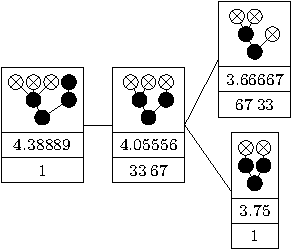
\includegraphics{p3/hlf_not_optimal/001112_hlf_subopt.pdf}
    \caption{Suboptimal HLF run}
  \end{subfigure}
  \begin{subfigure}{.45\linewidth}
    \centering
    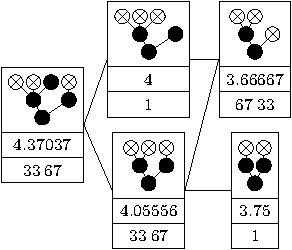
\includegraphics{p3/hlf_not_optimal/001112_hlf_opt.pdf}
    \caption{Optimal HLF run. This is also the overal optimal schedule.}
    \label{fig:hlf-001112-optimal-version}
  \end{subfigure}
  \caption{HLF on $(0,0,1,1,1,2)$. Different runs of HLF do not necessarily produce the same result.}
  \label{fig:hlf-001112}
\end{figure}

Because HLF can produce different run times depending which task it has chosen, it is clear that HLF in its raw form can not be optimal. The following section reveals even more.

\subsection{Examples where HLF is strictly suboptimal}
\label{sec:p3-suboptimal-hlf-strictly-suboptimal}

The example from figure \ref{fig:hlf-001112-optimal-version} shows the optimal run. We observe that this run is a specific instance of HLF, because at each point of time, always tasks with the highest level numbers are chosen.

However, there are intrees, where \emph{no} HLF-run is optimal. Figures \ref{fig:hlf-vs-opt-0012346688}, \ref{fig:hlf-vs-opt-0012446788} and \ref{fig:hlf-vs-opt-00123455799} show some examples for which this is exactly the case.

\begin{figure}[ht]
  \centering
  \begin{subfigure}{.45\linewidth}
    \centering
    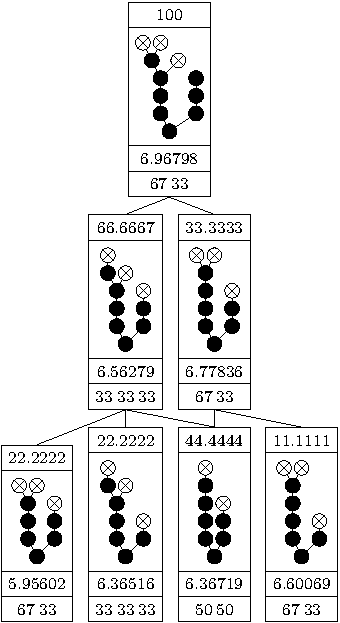
\includegraphics{p3/hlf_not_optimal/0012346688_subopt.pdf}
    \caption{HLF -- suboptimal}
  \end{subfigure}
  \begin{subfigure}{.45\linewidth}
    \centering
    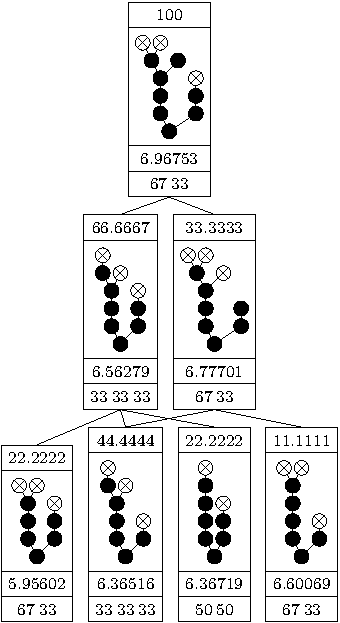
\includegraphics{p3/hlf_not_optimal/0012346688_opt.pdf}
    \caption{Optimal run is non-HLF}
  \end{subfigure}
  \caption{HLF vs. optimal solution for $(0,0,1,2,3,4,6,6,8,8)$}
  \label{fig:hlf-vs-opt-0012346688}
\end{figure}

\begin{figure}[ht]
  \centering
  \begin{subfigure}{.45\linewidth}
    \centering
    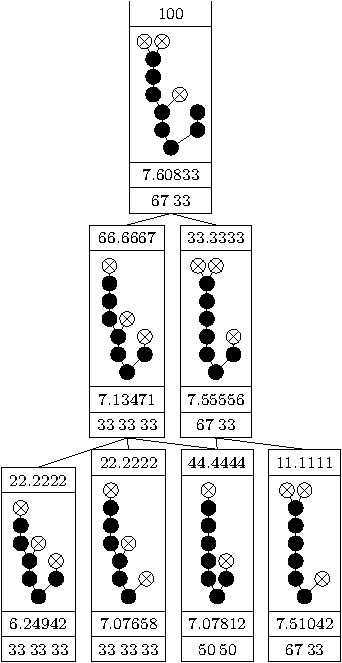
\includegraphics{p3/hlf_not_optimal/0012446788_subopt.pdf}
    \caption{HLF -- suboptimal}
  \end{subfigure}
  \begin{subfigure}{.45\linewidth}
    \centering
    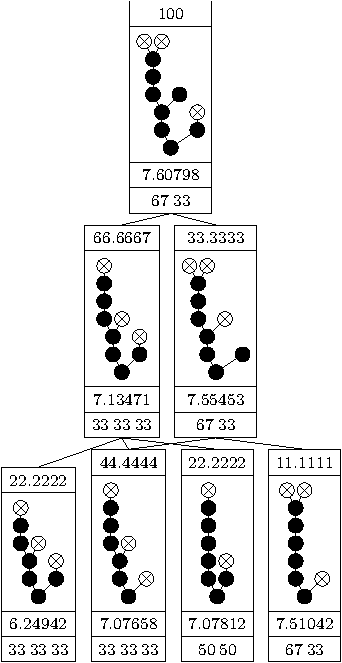
\includegraphics{p3/hlf_not_optimal/0012446788_opt.pdf}
    \caption{Optimal run is non-HLF}
  \end{subfigure}
  \caption{HLF vs. optimal solution for $(0,0,1,2,4,4,6,7,8,8)$ (taken from Ernst Mayr)}
  \label{fig:hlf-vs-opt-0012446788}
\end{figure}
\begin{figure}[ht]
  \centering
  \begin{subfigure}{.45\linewidth}
    \centering
    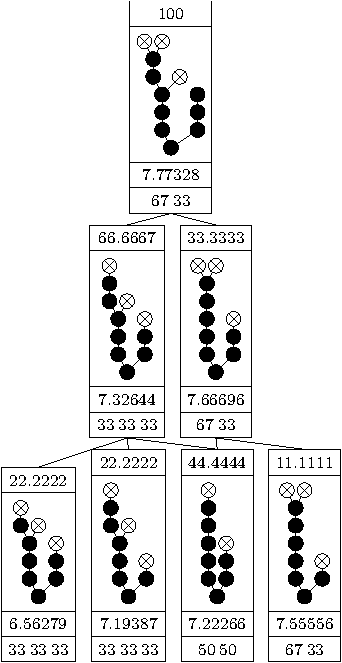
\includegraphics{p3/hlf_not_optimal/00123455799_subopt.pdf}
    \caption{HLF -- suboptimal}
  \end{subfigure}
  \begin{subfigure}{.45\linewidth}
    \centering
    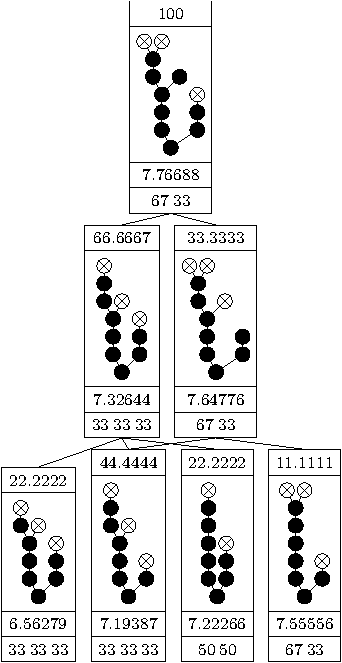
\includegraphics{p3/hlf_not_optimal/00123455799_opt.pdf}
    \caption{Optimal run is non-HLF}
  \end{subfigure}
  \caption{HLF vs. optimal solution for $(0,0,1,2,3,4,5,5,7,9,9)$ (taken from Chandy/Reynolds)}
  \label{fig:hlf-vs-opt-00123455799}
\end{figure}

\subsection{Quality of HLF}
\label{sec:suboptimal-hlf-quality}

We have seen that HLF is suboptimal in some cases, but experience shows that HLF is quite good in many cases. In fact \cite{journals/siamcomp/PapadimitriouT87} have shown that the following theorem holds:

\begin{theorem}
  There is a function $\beta: \mathbb{N} \mapsto \mathbb{R}^+_0$ with $\lim_{n\rightarrow \infty} \beta(n) = 0$ such that for each intree $I$ and an arbitrary HLF strategy $HLF$ we have
  \begin{equation*}
    T_{HLF}(I) \leq \inf_\pi\, T_{\pi}(I) \cdot \left( 1+\beta(N) \right),
  \end{equation*}
  where $T_{P}(I)$ denotes the expected run time for intree $I$ if it is scheduled by policy $P$, $N$ is the number of tasks in $I$ and the infimum is taken over all scheduling strategies $\pi$.
\end{theorem}

\begin{proof}
  See \cite{journals/siamcomp/PapadimitriouT87}.
\end{proof}

This result is quite useful because it shows that HLF is -- even if not optimal -- quite close as the number of tasks grows.

\subsection{Different categories of sub-optimality}
\label{sec:hlf-suboptimal-two-variants}

As we saw, there are two possibilities for the sub-optimality of HLF:

\begin{itemize}
\item \emph{Not each possible run} of HLF yields the same run time.
\item The optimal run has to choose a strict non-HLF task.
\end{itemize}

We use the following nomenclature: A strategy is called \emph{can-optimal} (a term already used in \cite{MoritzMaasDiploma}), if it \emph{might} result in an optimal schedule. A strategy that \emph{can not} produce an optimal solution is called \emph{strictly suboptimal} (or simply suboptimmal if it is clear from the context). 

It is a notable fact that there are many cases, where HLF is can-optimal. 

We use this distinction to (roughly) differentiate the following strategies into two categories: 

\begin{itemize}
\item The cases where HLF is strictly suboptimal lead us to several strategies that are presented in section \ref{sec:suboptimal-non-hlf-strategies}. These strategies are strict counterparts to HLF.
\item For the cases where HLF is can-optimal, we examined several strategies that try to determine which tasks should be chosen to minimize the expected run time. These strategies are presented in section \ref{sec:suboptimal-hlf-can-optimal-strategies}. These strategies can be seen as ``refinements'' of HLF such that HLF behaves better.
\end{itemize}

We will not only focus on particular strategies, but we will focus on which snapshots can be excluded or which particular structure snapshots might have. That is, the strategies we consider are in many cases ambiguous because they admit several possible choices. However, they do \emph{not} allow \emph{all} possible choices, thereby possibly reducing the amount of snapshots to examine. Not all strategies fall strictly into one of the groups -- we then put it into the category we found more insightful.

\section{(Dynamic) list scheduling}
\label{sec:suboptimal-strategies-list-scheduling}

List scheduling considers the current intree and generates a list of tasks sorted in such a way that the tasks that come first in the list shall be priorized and scheduled first, if possible. As shown by \cite{MoritzMaasDiploma}, dynamic list scheduling strategies can not be optimal for non-preemtive scheduling of intrees (whose tasks' run times are exponentially distributed) with three processors.

This can be seen by examining the intree $(0,0,1,1,1,2,2,2,2,3,6)$ as shown in figure \ref{fig:list-scheduling-counter-example}. Because the subtree shown in figure \ref{fig:list-schedule-counter-example-subtree} is optimally scheduled using other tasks than the one that have to be used when it is reached in the original schedule, there can not exist a dynamic list scheduling strategy that works for \emph{all} intrees.

Note that this also excludes HLF from being optimal.

\begin{figure}[ht]
  \centering
  \begin{subfigure}[b]{.45\textwidth}
    \centering
    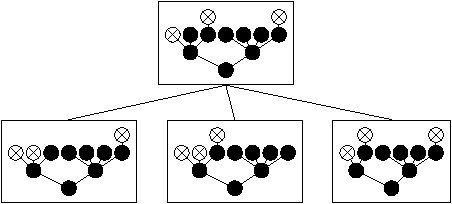
\includegraphics{p3/list_sched_0011122236_opt_sched.pdf}
    \caption{Optimal schedule for intree $(0,0,1,1,1,2,2,2,2,3,6)$.}
  \end{subfigure}
  \quad
  \begin{subfigure}[b]{.45\textwidth}
    \centering
    \vfill
    \includegraphics{p3/list_sched_subtree.pdf}
    \vfill
    \caption{This subtree of $(0,0,1,1,1,2,2,2,3,6)$ is optimally scheduled as shown, but in the optimal schedule for the original intree, it has to be scheduled in another way.}
    \label{fig:list-schedule-counter-example-subtree}
  \end{subfigure}
  \caption{A counterexample for list scheduling}
  \label{fig:list-scheduling-counter-example}
\end{figure}

That is, an optimal strategy has to consider which tasks are already scheduled from previous steps and can not rely \emph{only} on the current intree's structure. We experience this phenomenon in many intrees shown in this chapter. However, for the initial snapshot, we -- of course -- must rely on the structure of the intree. Thus, we will examine some strategies and inspect if the first snapshot of an optimal schedule adheres specific rules.

\section{Non-HLF strategies}
\label{sec:suboptimal-non-hlf-strategies}

We saw in section \ref{sec:hlf-p3-suboptimal} that there are examples where HLF is strictly suboptimal. We now present some strategies that we took into consideration and that we examined w.r.t. their optimality. 

We therefore considered optimal schedules and examined whether the initial snapshot (i.e. the initial choice of tasks) are formed upon a certain pattern.

These strategies are strongly different from HLF and rely upon the structure of the intree. None of the strategies considered lead us to strictly optimal results in all cases.

\subsection{``2-HLF plus 1''}
\label{sec:disproving-2hlf-plus-1}

We examined all intrees with up to 13 tasks, especially the cases where HLF is not optimal. Thereby, we obsered that in all cases where three tasks could be scheduled, the optimal solution scheduled two tasks, that could be chosen by HLF for two processors and only the third task \emph{might} be a task that would not have been chosen by HLF (see figures \ref{fig:hlf-vs-opt-0012346688}, \ref{fig:hlf-vs-opt-0012446788} and \ref{fig:hlf-vs-opt-00123455799} as particular instances of those). Thus, we examined whether an optimal scheduling strategy for three processors has always \emph{at most one} task that is non-HLF. Interestingly, there is an intree with 14 tasks, whose optimal schedule starts out by choosing the single topmost task and \emph{two} non-HLF tasks. This intree ($(0,0,1,2,2,3,3,6,8,9,10,11,12)$) is shown in figure \ref{fig:2-hlf-plus-one-not-optimal}. We can generalize this intree to a whole family of intrees where the optimal strategy initially chooses the single topmost task, and two lowest-level leaves by adding leaves along the longest chain. This results in intrees of the form $(0, 0, 1, 2, 3, 4, 4, 5, 5, 8, 10, 11, 12, 13, 14, 15,\dots)$.

\begin{figure}[ht]
  \centering
  \begin{subfigure}{.40\textwidth}
    \centering
    \includegraphics{p3/2hlf_suboptimal/0012233689101112_opt.pdf}
    \caption{Optimal schedule picking \emph{two} non-HLF tasks.}
  \end{subfigure}
  \begin{subfigure}{.58\textwidth}
    \centering
    \includegraphics{p3/2hlf_suboptimal/0012233689101112_subopt.pdf}
    \caption{HLF-Schedule}
  \end{subfigure}
  \caption{Intree $(0,0,1,2,2,3,3,6,8,9,10,11,12)$ requires the optimal schedule to start out by choosing two non-HLF tasks.}
  \label{fig:2-hlf-plus-one-not-optimal}
\end{figure}

\subsection{Only highest or lowest leaves}
\label{sec:disproving-only-highest-or-lowest-leaves}

The trees we examined so far resulted in schedules that picked only combinations \emph{highest leaves and lowest leaves} possible. Thus, we were tempted to think that an optimal schedule chooses only topmost tasks or leaves whose level is minimal (among all leaves). However, this is not a criterion for an optimal schedule, as we can observe by scheduling the 14-tasks-intree $(0,0,0,2,3,4,5,7,7,9,10,10,12)$, which is shown in figure \ref{fig:only-high-or-low-not-optimal}. For this intree, we have to schedule two topmost tasks and one task on level 3, but there is one unscheduled task remaining on level 1.

\begin{figure}[ht]
  \centering
  \begin{subfigure}{.45\textwidth}
    \centering
    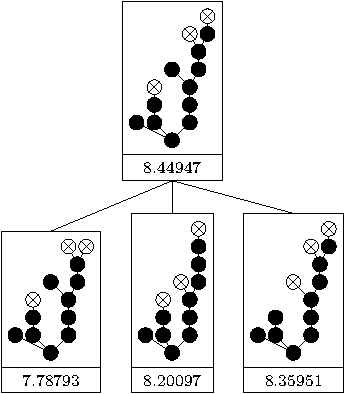
\includegraphics{p3/only_high_or_low/0002345779101012_opt.pdf}
    \caption{Optimal schedule picking a non-HLF task that is also not the lowest possible.}
  \end{subfigure}
  \quad
  \begin{subfigure}{.45\textwidth}
    \centering
    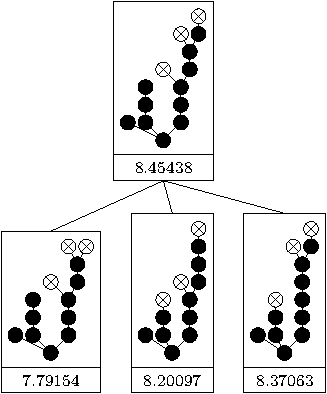
\includegraphics{p3/only_high_or_low/0002345779101012_subopt.pdf}
    \caption{Suboptimal HLF-Schedule.}
  \end{subfigure}
  \caption{Intree $(0,0,0,2,3,4,5,7,7,9,10,10,12)$ shows that there are intrees where an optimal schedule has to choose a non-HLF task that has a higher level than some non-chosen task.}
  \label{fig:only-high-or-low-not-optimal}
\end{figure}

\section{Refining can-optimal HLF}
\label{sec:suboptimal-hlf-can-optimal-strategies}

As mentioned in section \ref{sec:hlf-suboptimal-two-variants}, there are many cases where HLF is \emph{can-optimal}, i.e. where the optimal schedule always has tasks of the highest levels scheduled, but not each HLF schedule is optimal. This results from situations where HLF can choose one from several task as the next task to be scheduled. We describe some strategies that try to eliminate these ambiguities and give counterexamples that show that these strategies are not optimal.

\subsection{``As few free paths as possible''}
\label{sec:disproving-hlf-no-free-chain}

(For now,) we call a path from the root to a leaf (i.e. a ready task) $t$ \emph{free} if $t$ is not scheduled.

One might be tempted to think that it should be the foremost goal to exploit parallelism as good as possible and that this might be acchieved by choosing the currently scheduled tasks in a manner such that as few free paths as possible in an optimal schedule. That is, we choose the leaves in a way so that the ends of as many different paths as possible are scheduled. This strategy was the first that came to our mind and was inspired by looking at the counterexamples against HLF depicted in figures \ref{fig:hlf-001112}, \ref{fig:hlf-vs-opt-0012346688}, \ref{fig:hlf-vs-opt-0012446788} and \ref{fig:hlf-vs-opt-00123455799}. We observe for these intrees that the optimal schedules has no as few free chains as possible.

However, there are examples where the optimal contains snapshots that do not adhere this property. Consider e.g. the tree $(0,0,0,1,1,1,2,2,3)$ (figure \ref{fig:hlfnfc-is-not-optimal} compares the optimal schedule to the no-free-paths schedule).

\begin{figure}[ht]
  \centering
  \begin{subfigure}{.45\textwidth}
    \centering
    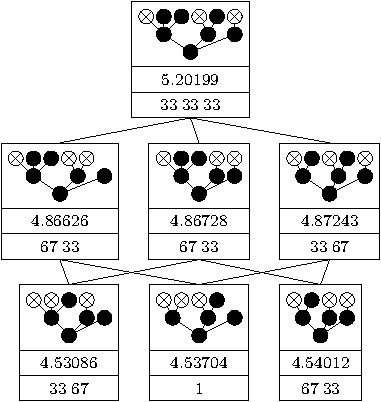
\includegraphics{p3/hlfnfc_not_optimal/000111223_hlfnfc.pdf}
    \caption{HLF schedule while choosing tasks such that there are as few free paths as possible -- overall run time of 5.20199.}
  \end{subfigure}
  \quad
  \begin{subfigure}{.45\textwidth}
    \centering
    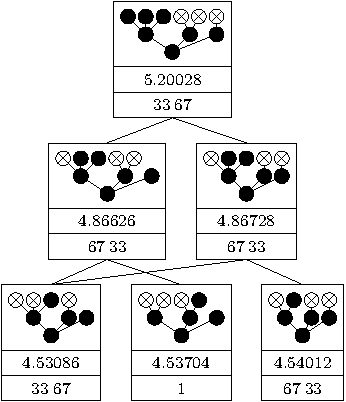
\includegraphics{p3/hlfnfc_not_optimal/000111223_opt.pdf}
    \caption{Optimal schedule (run time 5.20028) has three free paths at the beginning.}
  \end{subfigure}
  \caption{HLF with as few free paths as possible is not necessarily optimal.}
  \label{fig:hlfnfc-is-not-optimal}
\end{figure}

\subsection{Subtree with minimum number of topmost tasks}
\label{sec:suboptimal-hlf-can-optimal-subtree-fewest-toptasks}

If we consider the intree $(0,0,0,1,1,1,2,2,3)$, we have seen that an optimal schedule picks 7,8 and 9 as initially scheduled tasks (see figure \ref{fig:hlfnfc-is-not-optimal}). Moreover, in many cases, topmost-tasks that are the \emph{single direct predecessor} of their respective direct successor, are chosen by an optimal schedule.

These facts lead us to the suspicion that -- if we have an intree for which HLF is can-optimal -- (informally) we should pick the subtrees with the lowest number of topmost tasks. 

In this context, it is important to exactly describe which subtree we are talking about. Therefore, we employ the following definition:

\begin{definition}[Toptask-maximal subtree for a leaf]
  Let $t$ be a leaf of an intree $I$ and let $p=(t, t_1, t_2, t_3, \dots, r)$ be the path from $t$ to the root $r$.

  The \emph{toptask-maximal subtree for a leaf} $t$ is the subtree rooted at the \emph{lowest} task $t^*$ within $p$ that is not $t$ and that does \emph{not} contain more topmost tasks than the subtree rooted at the predecessor of $t^*$ within $p$.
\end{definition}

As an example, consider the following intree (remember that topmost tasks are defined to be the tasks whose levels are at least as large as the level of \emph{any} task in the intree --- see section \ref{sec:foundations-graph-theory}):

\begin{center}
  \begin{tikzpicture}[scale=.6, anchor=south]
    \node[circle, scale=0.9, draw] (tid0) at (3,1.5){0};
    \node[circle, scale=0.9, draw] (tid1) at (2.25,3){1};
    \node[circle, scale=0.9, draw] (tid2) at (1.5,4.5){3};
    \node[circle, scale=0.9, draw] (tid7) at (0.15,6){6};
    \node[circle, scale=0.9, draw] (tid10) at (1.5,6){7};
    \draw[ thick](tid2) -- (tid7);
    \draw[ thick](tid2) -- (tid10);
    \node[circle, scale=0.9, draw] (tid3) at (3.9,4.5){4};
    \node[circle, scale=0.9, draw] (tid5) at (2.85,6){8};
    \node[circle, scale=0.9, draw] (tid6) at (2.85,7.5){\small 10};
    \draw[ thick](tid5) -- (tid6);
    \draw[ thick](tid2) -- (tid5);
    \draw[ thick](tid1) -- (tid2);
    \draw[ thick](tid1) -- (tid3);
    \node[circle, scale=0.9, draw] (tid4) at (5.25,3){2};
    \node[circle, scale=0.9, draw] (tid9) at (4.3,6){9};
    \draw[ thick](tid3) -- (tid9);
    \node[circle, scale=0.9, draw] (tid11) at (4.3,7.5){11};
    \draw[ thick](tid11) -- (tid9);
    \node[circle, scale=0.9, draw] (tid8) at (5.25,4.5){5};
    \draw[ thick](tid4) -- (tid8);
    \draw[ thick](tid0) -- (tid1);
    \draw[ thick](tid0) -- (tid4);
  \end{tikzpicture}
\end{center}

The maximal subtree for leaf 10 is the subtree rooted at node 3, which can be derived as follows:
\begin{itemize}
\item The path from 10 to the root 0 is given by $p=(10,8,3,1,0)$.
\item We consider the subtrees rooted at the tasks along this path, and denote the subtree rooted at node $x$ by $I_x$:
  \begin{itemize}
  \item The subtree rooted at 10 (called $I_{10}$) contains only the topmost task 10.
  \item Subtree $I_8$ contains only topmost task 10.
  \item Subtree $I_3$ still contains only 10 as the topmost task (it introduces only a new leaf, namely 7).
  \item Subtree $I_1$ contains 10 \emph{and} 11 as topmost tasks.
  \end{itemize}
\item As seen, task 3 is the lowest task within $p$ that does not contain more topmost tasks than its predecessor (in the path from the leaf to the root).
\end{itemize}

A strategy for cases where HLF is can-optimal now might be to resolve HLF-ambiguities as follows:
\begin{itemize}
\item Generate all possible choices that could result from HLF.
\item For each topmost task, compute the topmost-maximal subtree.
\item Prefer topmost tasks whose topmost-maximal subtrees contain fewer topmost tasks.
\end{itemize}

The last step in the above explanation can be viewed as follows: We first create all possible choices of topmost tasks and then only pursue those, where there is no topmost-maximal subtree that has unscheduled topmost tasks.

This strategy seems to do a good job in many cases, but can be seen to be false by examining the optimal schedule for the following intree with 18 tasks: $(0,0,1,1,2,3,3,4,5,7,8,9,9,11,13,13,13)$. It is shown in figure \ref{fig:subtree-with-fewest-toptasks-suboptimal}.

\emph{Remark:} We did not specify what should be done if there are several maximal subtrees with the same number of topmost tasks, but our counterexample suffices that this strategy does not work optimally even if there are no maximal subtrees with the same number of nodes.

\begin{figure}[ht]
  \centering
  \begin{subfigure}{.45\textwidth}
    \centering
    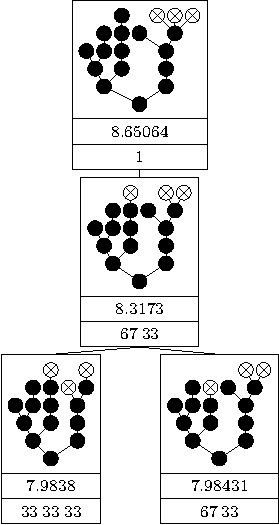
\includegraphics{p3/subtree_with_fewest_toptasks/subtree_with_fewest_toptasks_opt.pdf}
    \caption{Optimal schedule picking a subtree with three topmost tasks.}
  \end{subfigure}
  \quad
  \begin{subfigure}{.45\textwidth}
    \centering
    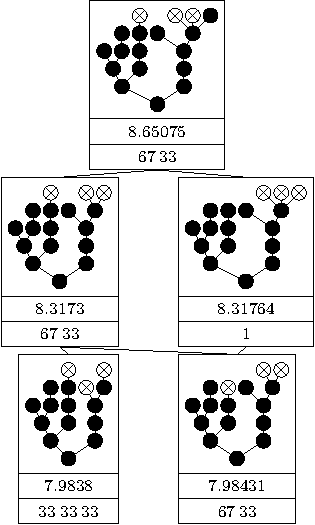
\includegraphics{p3/subtree_with_fewest_toptasks/subtree_with_fewest_toptasks_subopt.pdf}
    \caption{If we initially start with tasks as shown, this is the best schedule that can be obtained.}
  \end{subfigure}
  \caption{Intree $(0,0,1,1,2,3,3,4,5,7,8,9,9,11,13,13,13)$: For this intree, the optimal schedule chooses all tasks from a subtree with three topmost tasks and chooses none of the subtree with only one topmost tasks.}
  \label{fig:subtree-with-fewest-toptasks-suboptimal}
\end{figure}

\subsection{Subtree with maximum or minimum number of leaves}
\label{sec:suboptimal-hlf-can-optimal-subtree-fewest-leaves}

It can be quickly seen that slightly altering the strategy given in section \ref{sec:suboptimal-hlf-can-optimal-subtree-fewest-toptasks} in the sense that we do not concentrate on the number of \emph{topmost tasks} in a maximal subtree, but more generraly on the number of \emph{leaves} in a maximal subtree, does not yield a successful strategy. We adapt the notion of topmost-maximal subtrees in a straightforward manner:

\begin{definition}[Leaf-maximal subtree for a leaf]
  Let $t$ be a leaf of an intree $I$ and let $p=(t, t_1, t_2, t_3, \dots, r)$ be the path from $t$ to the root $r$.

  The \emph{leaf-maximal subtree for a leaf} $t$ is the subtree rooted at the \emph{lowest} task $t^*$ within $p$ that is not $t$ and that does \emph{not} contain more leaves than the predecessor of $t^*$ within $p$.
\end{definition}

\begin{description}
\item [Preferring leaf-maximal subtrees with fewer leaves] Figure \ref{fig:subtree-with-fewest-toptasks-suboptimal} shows that this strategy is not optimal, since the optimal solution prefers a subtree with four leaves over one with only three leaves.
  \emph{Remark:} The tree $(0,0,1,1,2,3,3,4,5,7,8,9,9,11,13,13,13)$ in particular shows that there are situations where a topmost task that is the \emph{only} requirement for its predecessor is initially \emph{not} scheduled in the optimal case. During our research we have experienced that this is a very rare situation.
\item [Preferring leaf-maximal subtrees with more leaves] One of our first examples, the intree $(0,0,0,1,1,1,2,2,3)$ (see figure \ref{fig:hlfnfc-is-not-optimal}) already shows that this strategy is not optimal in general.
\end{description}

\subsection{Preferring root's predecessors with longest processing time}
\label{sec:suboptimal-hlf-can-roots-longest-predecessors}

We also tried a recursive approach that decomposed an intree as follows: We separate the intrees rooted at the predecessors of the root. This way, we get a whole set of intrees. For each subtree, we now compute the optimal schedule and, moreover, the expected processing time -- assuming three processors in each individual subtree. The schedule for the whole intree then shall prefer subtrees whose expected processing time is the longest.

We were tempted to conjecture this because of the intree $(0,0,1,1,2,3,3,4,5,7,8,9,9,11,13,13,13)$ whose optimal schedule starts shown in figure \ref{fig:subtree-with-fewest-toptasks-suboptimal}. If we decompose this intree into its parts, we see that the subtree whose expected run time is maximal is the one whose tasks are initially scheduled in the optimal schedule (see figure \ref{fig:reasoning-for-longest-root-subtree}).

\begin{figure}[ht]
  \centering
  \begin{subfigure}{.45\textwidth}
    \centering
    \begin{tikzpicture}[scale=.2, anchor=south]
      \node[circle, scale=0.75, fill] (tid0) at (5.25,1.5){};
      \node[circle, scale=0.75, fill] (tid1) at (2.25,3){};
      \node[circle, scale=0.75, fill] (tid3) at (1.5,4.5){};
      \node[circle, scale=0.75, fill] (tid6) at (0.75,6){};
      \node[circle, scale=0.75, fill] (tid7) at (2.25,6){};
      \node[circle, scale=0.75, fill] (tid10) at (2.25,7.5){};
      \draw[](tid7) -- (tid10);
      \draw[](tid3) -- (tid6);
      \draw[](tid3) -- (tid7);
      \node[circle, scale=0.75, fill] (tid4) at (3.75,4.5){};
      \node[circle, scale=0.75, fill] (tid8) at (3.75,6){};
      \node[circle, scale=0.75, fill] (tid11) at (3.75,7.5){};
      \node[circle, scale=0.75, fill] (tid14) at (3.75,9){};
      \draw[](tid11) -- (tid14);
      \draw[](tid8) -- (tid11);
      \draw[](tid4) -- (tid8);
      \draw[](tid1) -- (tid3);
      \draw[](tid1) -- (tid4);
      \node[circle, scale=0.75, fill] (tid2) at (7.5,3){};
      \node[circle, scale=0.75, fill] (tid5) at (7.5,4.5){};
      \node[circle, scale=0.75, fill] (tid9) at (7.5,6){};
      \node[circle, scale=0.75, fill] (tid12) at (5.25,7.5){};
      \node[circle, scale=0.75, fill] (tid13) at (8.25,7.5){};
      \node[circle, scale=0.75, fill, task_scheduled] (tid15) at (6.75,9){};
      \node[circle, scale=0.75, fill, task_scheduled] (tid16) at (8.25,9){};
      \node[circle, scale=0.75, fill, task_scheduled] (tid17) at (9.75,9){};
      \draw[](tid13) -- (tid15);
      \draw[](tid13) -- (tid16);
      \draw[](tid13) -- (tid17);
      \draw[](tid9) -- (tid12);
      \draw[](tid9) -- (tid13);
      \draw[](tid5) -- (tid9);
      \draw[](tid2) -- (tid5);
      \draw[](tid0) -- (tid1);
      \draw[](tid0) -- (tid2);
    \end{tikzpicture}  
    \caption{Intree with initially scheduled tasks (for optimal schedule).}
  \end{subfigure}
  \quad
  \begin{subfigure}{.45\textwidth}
    \centering
    \begin{tikzpicture}[scale=.2, anchor=south]
      \node[circle, scale=0.75, fill] (tid1) at (2.25,3){};
      \node[circle, scale=0.75, fill] (tid3) at (1.5,4.5){};
      \node[circle, scale=0.75, fill] (tid6) at (0.75,6){};
      \node[circle, scale=0.75, fill] (tid7) at (2.25,6){};
      \node[circle, scale=0.75, fill] (tid10) at (2.25,7.5){};
      \draw[](tid7) -- (tid10);
      \draw[](tid3) -- (tid6);
      \draw[](tid3) -- (tid7);
      \node[circle, scale=0.75, fill] (tid4) at (3.75,4.5){};
      \node[circle, scale=0.75, fill] (tid8) at (3.75,6){};
      \node[circle, scale=0.75, fill] (tid11) at (3.75,7.5){};
      \node[circle, scale=0.75, fill] (tid14) at (3.75,9){};
      \draw[](tid11) -- (tid14);
      \draw[](tid8) -- (tid11);
      \draw[](tid4) -- (tid8);
      \draw[](tid1) -- (tid3);
      \draw[](tid1) -- (tid4);
      \node at (2.25, 0){5.67991};
      \begin{scope}[xshift=4cm]
        \node[circle, scale=0.75, fill] (tid2) at (7.5,3){};
        \node[circle, scale=0.75, fill] (tid5) at (7.5,4.5){};
        \node[circle, scale=0.75, fill] (tid9) at (7.5,6){};
        \node[circle, scale=0.75, fill] (tid12) at (5.25,7.5){};
        \node[circle, scale=0.75, fill] (tid13) at (8.25,7.5){};
        \node[circle, scale=0.75, fill] (tid15) at (6.75,9){};
        \node[circle, scale=0.75, fill] (tid16) at (8.25,9){};
        \node[circle, scale=0.75, fill] (tid17) at (9.75,9){};
        \draw[](tid13) -- (tid15);
        \draw[](tid13) -- (tid16);
        \draw[](tid13) -- (tid17);
        \draw[](tid9) -- (tid12);
        \draw[](tid9) -- (tid13);
        \draw[](tid5) -- (tid9);
        \draw[](tid2) -- (tid5);
        \node at (7.5, 0){6.83333};
      \end{scope}
    \end{tikzpicture}  
    \caption{Removing the root yields two subtrees with optimal expected runtimes (for three processors) as noted.}
  \end{subfigure}
  \caption{Intree $(0,0,1,1,2,3,3,4,5,7,8,9,9,11,13,13,13)$ and its corresponding subtrees rooted at the root's predecessors}
  \label{fig:reasoning-for-longest-root-subtree}
\end{figure}

Once again, this strategy can be shown to be suboptimal by considering $(0,0,0,1,1,1,2,2,3)$ (as depicted in figure \ref{fig:hlfnfc-is-not-optimal}) whose root has the following three predecessor intrees.

\begin{center}
  \begin{tikzpicture}[scale=.3]
    \begin{scope}
      \node[circle, fill, scale=.5] (0) at (0,0){};
      \node[circle, fill, scale=.5] (1) at (-1,1){};
      \node[circle, fill, scale=.5] (2) at (0,1){};
      \node[circle, fill, scale=.5] (3) at (1,1){};
      \draw(0)--(1);
      \draw(0)--(2);
      \draw(0)--(3);
      \node at (0, -1.5){2.83333};
    \end{scope}
    \begin{scope}[xshift=5cm]
      \node[circle, fill, scale=.5] (0) at (0,0){};
      \node[circle, fill, scale=.5] (1) at (-.5,1){};
      \node[circle, fill, scale=.5] (3) at (.5,1){};
      \draw(0)--(1);
      \draw(0)--(3);
      \node at (0, -1.5){2.5};
    \end{scope}
    \begin{scope}[xshift=10cm]
      \node[circle, fill, scale=.5] (0) at (0,0){};
      \node[circle, fill, scale=.5] (1) at (0,1){};
      \draw(0)--(1);
      \node at (0, -1.5){2};
    \end{scope}
  \end{tikzpicture}
\end{center}

For $(0,0,0,1,1,1,2,2,3)$ the optimal schedule initially chooses the tasks 7,8 and 9 (the respective subtrees have run times 2.5 and 2).

\subsection{Preferring root's predecessors with shortest processing time}
\label{sec:suboptimal-preferring-root-predecessors-shortest-time}

It is clear that the opposite of the strategy from section \ref{sec:suboptimal-hlf-can-roots-longest-predecessors}, namely preferring those subtrees whose processing time is shortest, does also not yield correct results. This can be easily seen by considering the intree $(0,1,2,3,0,5,6,0,8,0)$ that is optimally scheduled by HLF (see section \ref{sec:p3-parallel-chains} for a proof) and whose root has the three following predecessors:

\begin{center}
  \begin{tikzpicture}[scale=.3]
    \begin{scope}[xshift=15cm]
      \node[circle, fill, scale=.5] (0) at (0,0){};
      \node[circle, fill, scale=.5] (1) at (0,1){};
      \node[circle, fill, scale=.5] (2) at (0,2){};
      \node[circle, fill, scale=.5] (3) at (0,3){};
      \draw(0)--(3);
      \node at (0, -1.5){4};
    \end{scope}
    \begin{scope}[xshift=20cm]
      \node[circle, fill, scale=.5] (0) at (0,0){};
      \node[circle, fill, scale=.5] (1) at (0,1){};
      \node[circle, fill, scale=.5] (2) at (0,2){};
      \draw(0)--(2);
      \node at (0, -1.5){3};
    \end{scope}
    \begin{scope}[xshift=25cm]
      \node[circle, fill, scale=.5] (0) at (0,0){};
      \node[circle, fill, scale=.5] (1) at (0,1){};
      \draw(0)--(1);
      \node at (0, -1.5){2};
    \end{scope}
    \begin{scope}[xshift=30cm]
      \node[circle, fill, scale=.5] (0) at (0,0){};
      \draw(0)--(0);
      \node at (0, -1.5){1};
    \end{scope}
  \end{tikzpicture}
\end{center}

\subsection{``Filling up subtrees''}
\label{sec:suboptimal-filling-subtrees}

We observed that (for three processors) an optimal schedule looks as if it chose certain subtrees and ``filled them up one after another''. This is probably most concise formalized as the following pattern:

\begin{itemize}
\item Identify disjoint leaf-maximal (or topmost-maximal) subtrees of the whole intree.
\item Assign priorities to the subtrees so they are sorted according to this priority (thus, we have a sequence of subtrees $S_1,\dots,S_r$).
\item Schedule as many tasks from $S_1$ as possible. If all ready tasks in $S_1$ are scheduled, schedule as many tasks as possible in $S_2$. If all tasks in $S_2$ are scheduled, schedule as many tasks as possible in $S_3$.
\end{itemize}
%In an optimal schedule, we can -- without loss of generality -- assume that it is \emph{not} the case that there are two distinct scheduled tasks $x$ and $y$ with different successors and each of them having a non-scheduled, but ready task.

An alternative formulation of the above strategy states that there is at most one task having both scheduled and non-scheduled predecessors that are leaves. 

We have already seen that there are optimal schedules violating this property, e.g. the intree $(0,0,0,1,1,2,2,3)$. But for those intrees, there is another schedule having \emph{exact the same} run time but fulfilling the property.

The example intree $(0,0,0,1,1,2,2,3)$ admits two different schedules (one beginning with tasks 4,5,8 and the other beginning with 4,6,8) that have exactly the same run time (see figure \ref{fig:filling-up-without-loss-of-generality}). The reason is that both schedules result in equivalent snapshots with the same probabilities after the first task finishes.

\begin{figure}[th]
  \centering
  \begin{subfigure}{.45\textwidth}
    \centering
    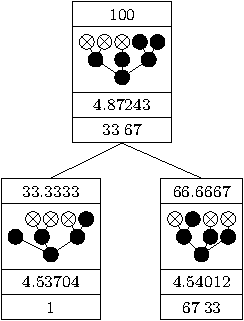
\includegraphics{p3/suboptimal/000111223_opt458.pdf}
    \caption{Optimal schedule starting with tasks 4,5 and 8.}
  \end{subfigure}
  \quad
  \begin{subfigure}{.45\textwidth}
    \centering
    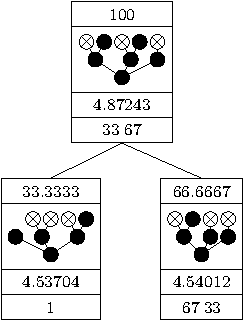
\includegraphics{p3/suboptimal/000111223_opt468.pdf}
    \caption{Optimal schedule starting with tasks 4,6 and 8.}
  \end{subfigure}
  \caption{The intree $(0,0,0,1,1,2,2,3)$ has two different schedules reaching the optimum expected run time.}
  \label{fig:filling-up-without-loss-of-generality}
\end{figure}

For trees with fewer than 12 tasks, we could not find any tree that violated our conjecture, but the intree $(0,0,0,2,2,3,5,5,6,6,6)$ has the interesting property that the optimal schedule for this intree has to schedule tasks such that the intree contains two tasks that have as well scheduled as non-scheduled but ready predecessors. Figure \ref{fig:filling-op-is-not-strictly-optimal} shows the first steps of an optimal schedule for this intree.

\begin{figure}[th]
  \centering
  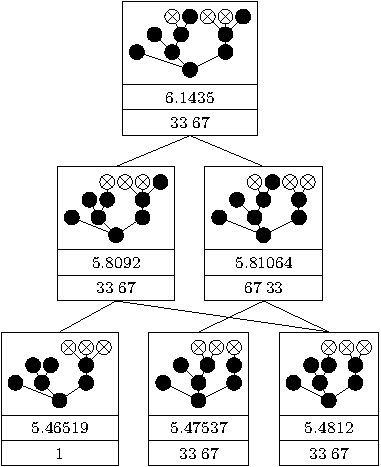
\includegraphics{p3/suboptimal/00022355666_optimal_no_fill_up.pdf}
  \caption{The optimal schedule for $(0,0,0,2,2,3,5,5,6,6,6)$ has two tasks (5 and 6) that have both scheduled and non-scheduled leaves as predecessors.}
  \label{fig:filling-op-is-not-strictly-optimal}
\end{figure}

\emph{Remark:} Surprisingly, every subtree of $(0,0,0,2,2,3,5,5,6,6,6)$ fulfills the conjecture that there is at most one task that has both scheduled and non-scheduled leaves as predecessors (during the whole schedule). This shows that even task that \emph{might seem} of minor impact for the first choices, might be relevant to the question which tasks are chosen in the optimal schedule.

\section{Maximizing 3-processor-time, minimizing 1-processor time}
\label{sec:p3-disproving-long-p3-and-short-p1-time}

Up to now, we maily focused on the structure of the current intree to derive strategies --- which all turned out to be (not strictly, but still) suboptimal. We now inspect another, more involved approach.

If we have three processors in total, we can split the total run time into three parts: The time where all three processors are processing tasks, the time where one processor is idle and two are working, and the time where only one processor is working.

%We first define some variants of run time. We consider the overall run time and the time where -- within a schedule of an intree -- exactly $p$ processors are working (i.e. where exactly $p$ tasks are scheduled).

\begin{definition}[Run time and its variants]
  We denote by $T$ the expected run time for a schedule associated with an intree. 
  Moreover, we denote the time where exactly $p$ taks are scheduled by $T_p$.
\end{definition}

Note that $T$ actually describes an \emph{expected value}. Because of the linearity of expectation, we have that -- for three processors -- $T=T_1 + T_2 + T_3$. If we want to construct an optimal schedule for three processors, we might be tempted to think that (at least) one of the two following criteria should be fulfilled for the optimal schedule:

\begin{description}
\item[P3L] For the optimal schedule, $T_3$ should be maximal (over all schedules), i.e. we should exploit three processors as long as possible (in the expectation).
\item[P1S] For the optimal schedule, $T_1$ should be minimal (over all schedules), i.e. we should try to keep the expected time for which only one processor is working as short as possible.
\end{description}

Surprisingly, \emph{both} of them are wrong (at least if considered separately).

\subsection{Maximizing $T_3$}
\label{sec:p3-disproving-long-p3}

Figure \ref{fig:p3-p3l-suboptimal-example} shows an example, where the optimal schedule keeps three processors busy for expected 0.77777 time steps, while a suboptimal schedule keeps three processors busy for a longer expected time, namely about 0.851852 time steps.

From this we can conclude that it may be advantageous in some cases to accept a shorter time with three busy processors, thereby possibly also decreasing the time where only one processor is busy.

\begin{figure}[ht]
  \centering
  \begin{subfigure}{.45\linewidth}
    \centering
    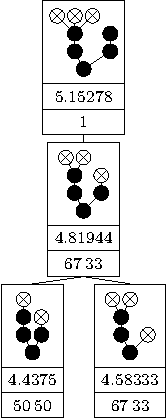
\includegraphics{p3/keep_3_busy/three_busy_opt.pdf}
    \caption{Optimal schedule. Keeps three processors busy for $7/9\approx 0.78$ time steps ($(T_3, T_2, T_1)=(7/9, 31/24, 37/12)$).}
  \end{subfigure}
  \quad
  \begin{subfigure}{.45\linewidth}
    \centering
    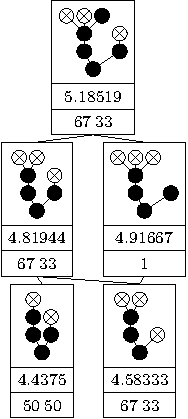
\includegraphics{p3/keep_3_busy/three_busy_subopt.pdf}
    \caption{This suboptimal schedule keeps three processors busy for expectedly $0.851852$ time steps ($(T_3, T_2, T_1)=(23/27,10/9,29/9)$).}
  \end{subfigure}
  \caption{An intree that shows that an optimal P3 schedule needs not keep busy three processors as long as possible. Snapshots with fewer than 6 tasks omitted since they have at most two tasks to be schedlued can be (optimally) processed via ordinary HLF.}
  \label{fig:p3-p3l-suboptimal-example}
\end{figure}

\subsection{Minimizing $T_1$}
\label{sec:p3-disproving-short-p1}

The ``other direction'', i.e. minimizing the time where only one processor is busy, still is suboptimal.
Figure \ref{fig:p3-p1s-suboptimal-example} shows an intree with the property that the optimal schedule has an expected timespan of roughly 2.59259, within which only one processor is busy. On the other hand, a suboptimal schedule has a timespan of roughly 2.55555 within which only one processor is busy.

\begin{figure}[ht]
  \centering
  \begin{subfigure}{.45\linewidth}
    \centering
    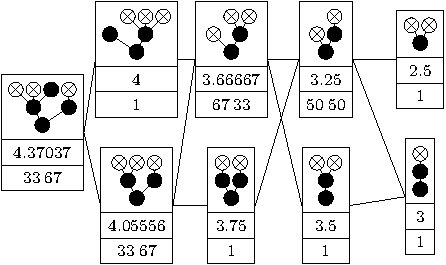
\includegraphics{p3/keep_1_unbusy/one_unbusy_opt.pdf}
    \caption{Optimal schedule. For expectedly $70/27\approx 2.59$ time steps, only one processor is busy $(T_3, T_2, T_1)=(23/27, 25/27, 70/27)$.}
  \end{subfigure}
  \quad
  \begin{subfigure}{.45\linewidth}
    \centering
    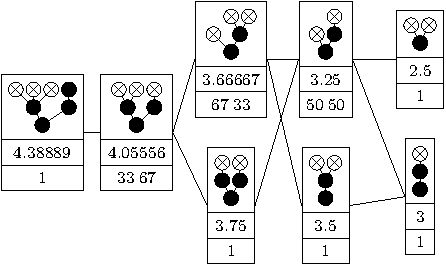
\includegraphics{p3/keep_1_unbusy/one_unbusy_subopt.pdf}
    \caption{This suboptimal schedule has an approximated timespan of $23/9\approx 2.55$ time steps, where only one processor is working ($(T_3, T_2, T_1)=(7/9,19/18,23/9)$).}
  \end{subfigure}
  \caption{An intree where the expected time with only one processor being busy is longer within the optimal schedule ($\approx 2.59259$) than within a suboptimal schedule ($\approx 2.555555$).}
  \label{fig:p3-p1s-suboptimal-example}
\end{figure}

This shows that it can be useful to accept a longer time with only one processor busy, probably acchieving a longer time span where three processors are busy.

\subsection{Maximizing $T_3$ \emph{or} minimizing $T_1$}
\label{sec:p3-suboptimality-maximizing-t3-and-minimizing-t1}

It can also be shown that even combining the two arguments -- in the sense that P3L \emph{or} P1S should be fulfilled for the optimal schedule -- is not correct. This can be observed by examining the intree $(0, 0, 1, 1, 2, 3, 3, 3)$. Figure \ref{fig:p3l-p1s-combo-suboptimal} shows this example.

\begin{figure}[ht]
  \centering
  \begin{subfigure}{.3\linewidth}
    \centering
    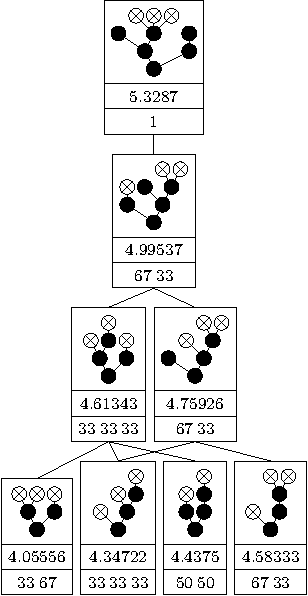
\includegraphics{p3/max_p3_min_p1/00112333opt.pdf}
    \caption{Optimal schedule. $(T_3^*,T_2^*,T_1^*)=(\frac{4}{3},\frac{217}{216},\frac{323}{108})$.}
  \end{subfigure}
  \quad
  \begin{subfigure}{.3\linewidth}
    \centering
    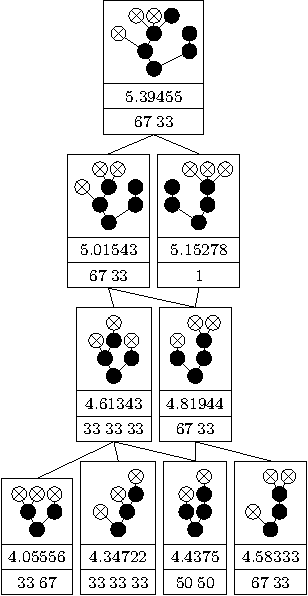
\includegraphics{p3/max_p3_min_p1/00112333t1min.pdf}
    \caption{Schedule with minimal $T_1$. $(T_3,T_2,T_1)=(\frac{290}{243},\frac{2369}{1944},\frac{2899}{972})$.}
  \end{subfigure}
  \quad
  \begin{subfigure}{.3\linewidth}
    \centering
    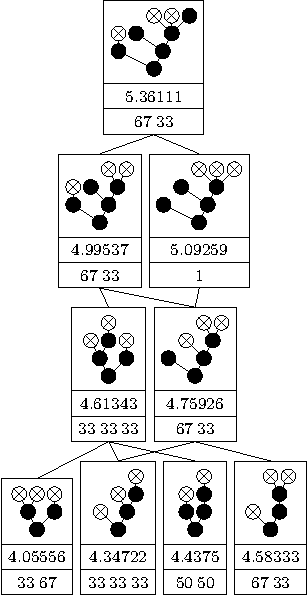
\includegraphics{p3/max_p3_min_p1/00112333t3max.pdf}
    \caption{Schedule with maximal $T_3$. $(T_3,T_2,T_1)=(\frac{110}{81},\frac{299}{324},\frac{499}{162})$.}
  \end{subfigure}
  \caption{A combination of P3L and P1S is not a criterion for an optimal schedule. The optimal schedule has $T_3^*=\frac{4}{3}\approx 1.333$ and $T_1^*=\frac{323}{108}\approx 2.99074$. One other (suboptimal) schedule has $T_1=\frac{2899}{972}\approx 2.98251 < T_1^*$, while still another schedule has $T_3=\frac{110}{81}\approx1.358025 > T_3^*$.}
  \label{fig:p3l-p1s-combo-suboptimal}
\end{figure}

\begin{corollary}
  Let $T^s$ denote the overall run time of a schedule $s$ and $T_1^s$, $T_2^s$ and $T_3^s$ be the times where exactly three, two and one tasks are scheduled within this schedule, respectively.

  Let $I$ be an intree and $S$ be the set of all schedules. Let $s^*$ be the optimal schedule, which has associated the optimal run time $T^*$, with $T_1^*, T_2^*, T_3^*$ being its parts.
  \begin{itemize}
  \item It may be the case that there is a schedule $s\in S$ such that $T_3^s \geq T_3^*$.
  \item It may be the case that there is a schedule $s\in S$ such that $T_1^s \leq T_1^*$.
  \end{itemize}
\end{corollary}

That is, it is not necessarily the case that $T_3$ is maximal for the optimal schedule, nor is it necessarily the case that $T_1$ is minimal for the optimal schedule.

However, after some investigation, we are tempted to conjecture the following.

\begin{conjecture}
  Let $I$, $T^s, T_1^s, T_2^s, T_3^s$ and $S$ be as defined above. Let $s^*$ be the optimal schedule for $I$ associated with the respective times $T_1^*, T_2^*, T_3^*$. Then, there is no schedule $s\in S$ such that
  \begin{equation*}
    T^s > T^* \wedge T_1^s \leq T_1^* \wedge T_3^s \geq T_3^*.
  \end{equation*}
\end{conjecture}

Even if this conjecture turns out to be true, it seems complex to transform this knowledge into a scheduling strategy that does something more significantly efficient than ``explore everything, and choose the best'', because $T_3, T_2$ and $T_1$ are not that easy to compute.

\section{Conclusion}
\label{sec:p3-conclusion}

Unfortunately, we did not find any strategy that always yields an optimal schedule. Of course, it is still possible to compute the optimal schedule by an exhaustive search.

During our research, we recognized some patterns that we are tempted to transform into conjectures. We were, however, not yet able to prove or disprove them. These conjectures might be used to reduce the number of snapshots that need to be examined by an exhaustive search used to compute the optimal snapshot.

This section shows the most important conjectures we found.

\begin{conjecture}
  \label{conj:as-many-topmost-as-possibly}
  An optimal schedule always schedules as many topmost tasks as possible.
\end{conjecture}

Please note that the above conjecture does not state anything about \emph{which} topmost tasks should be chosen in order to generate a schedule that is as good as possible. It can -- however -- drastically reduce the number of choices for the tasks to be scheduled. As an example, consider the following tree:

\begin{center}
  \begin{tikzpicture}[scale=.2]
    \node[circle, scale=0.75, fill] (tid0) at (7.5,1.5){};
    \node[circle, scale=0.75, fill] (tid1) at (0.75,3){};
    \node[circle, scale=0.75, fill] (tid2) at (5.25,3){};
    \node[circle, scale=0.75, fill] (tid4) at (2.25,4.5){};
    \node[circle, scale=0.75, fill] (tid5) at (3.75,4.5){};
    \node[circle, scale=0.75, fill] (tid8) at (3.75,6){};
    \draw[](tid5) -- (tid8);
    \node[circle, scale=0.75, fill] (tid6) at (6.75,4.5){};
    \node[circle, scale=0.75, fill] (tid9) at (6,6){};
    \node[circle, scale=0.75, fill] (tid13) at (5.25,7.5){};
    \node[circle, scale=0.75, fill] (tid14) at (6.75,7.5){};
    \draw[](tid9) -- (tid13);
    \draw[](tid9) -- (tid14);
    \node[circle, scale=0.75, fill] (tid10) at (8.25,6){};
    \node[circle, scale=0.75, fill] (tid15) at (8.25,7.5){};
    \draw[](tid10) -- (tid15);
    \draw[](tid6) -- (tid9);
    \draw[](tid6) -- (tid10);
    \draw[](tid2) -- (tid4);
    \draw[](tid2) -- (tid5);
    \draw[](tid2) -- (tid6);
    \node[circle, scale=0.75, fill] (tid3) at (12,3){};
    \node[circle, scale=0.75, fill] (tid7) at (12,4.5){};
    \node[circle, scale=0.75, fill] (tid11) at (9.75,6){};
    \node[circle, scale=0.75, fill] (tid12) at (12.75,6){};
    \node[circle, scale=0.75, fill] (tid16) at (11.25,7.5){};
    \node[circle, scale=0.75, fill] (tid17) at (12.75,7.5){};
    \node[circle, scale=0.75, fill] (tid18) at (14.25,7.5){};
    \draw[](tid12) -- (tid16);
    \draw[](tid12) -- (tid17);
    \draw[](tid12) -- (tid18);
    \draw[](tid7) -- (tid11);
    \draw[](tid7) -- (tid12);
    \draw[](tid3) -- (tid7);
    \draw[](tid0) -- (tid1);
    \draw[](tid0) -- (tid2);
    \draw[](tid0) -- (tid3);
  \end{tikzpicture}
\end{center}

This tree has 6 topmost tasks, but 10 leaves in total. If conjecture \ref{conj:as-many-topmost-as-possibly} is correct, then we can restrict ourselves to combinations of 6 topmost tasks -- being at most $\binom{6}{3}=20$ possible choices, in this particular case even only 6 due to equivalence of snapshots. In contrast, considering all 10 leaves, we have 48 possible choices in the above example.

Note that conjecture \ref{conj:as-many-topmost-as-possibly} also helps us to restrict the number of snapshots in another way: If we have to keep two tasks scheduled (because they were already scheduled in the previous step), we possibly do not need to examine all other tasks to be scheduled. If there are topmost tasks remaining, we can focus on them and do not need to examine non-topmost tasks.

Moreover, we are tempted to say the following:

\begin{conjecture}
  \label{conj:only-nontop-tasks-exchange-better}
  If for an intree only non-top tasks are scheduled, you can schedule any top-task instead of one non-top scheduled task to obtain a better run time.
\end{conjecture}

Conjecture \ref{conj:only-nontop-tasks-exchange-better} is not that useful in a direct application to reduce the number of snapshots needed to examine if we do an exhaustive search. However, it might be useful for proofs.

The main problems we faced when we tried to prove the above conjectures can be summarized as follows:
\begin{itemize}
\item If working with particular cases of intrees, the structure is not necessarily maintained over the induction step --- and if so, many case distinctions may be required.
\item Comparing different intrees seems to be quite cumbersome, especially if we do not know which tasks are scheduled.
\end{itemize}


%%% Local Variables:
%%% TeX-master: "../thesis.tex"
%%% End: 
\chapter{Properties of schedule DAGs and optimal schedules}
\label{chap:p3}

We now researching some properties of snapshot DAGs and optimal schedules. In particular, we will look at a particular non-trivial class of intrees, for which HLF is optimal.

\section{Properties of optimal schedules}
\label{sec:optimal-schedules-properties}

\subsection{Idle processors}
\label{sec:optimal-schedule-no-idleness}

As shown in \cite{chandyreynoldslargepaper1979}, it is known that an optimal scheduling strategy does not keep a processor idle if it could do some work. An intuitive explanation of this fact is as follows: Assume that there is a strategy that keeps a processor idle at some point even if there is a ready task $t$ that could be processed. Then, we construct a new strategy, that schedules $t$ (using the idle processor) and behaves like the original strategy. Then, it can be shown that this new strategy yields a smaller overall expected run time.

\subsection{Preemtive vs. non-preemtive scheduling}
\label{sec:optimal-schedules-preemtive}

\label{preemtiveness-explanation}
In section \ref{sec:schedules-problem-setting}, we mentioned that preemptive scheduling might yield better results than non-preemtive scheduling. As an example, \cite{MoritzMaasDiploma} shows the intree $(0,0,1,2,2,3,3,3,4,5)$. This intree is -- non-preemtively -- optimally processed by starting out with tasks 7, 8 and 9. However, we can acchieve a better overall runtime by initially scheduling 8, 9 and 10. Consider figure \ref{fig:preemtive-example-00111222} to compare both schedules.

\begin{figure}[ht]
  \centering
  \begin{subfigure}{.45\linewidth}
    \centering
    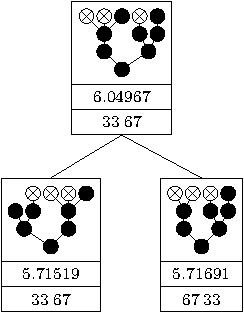
\includegraphics{p3/preemtive/0012233345_nonpreemtive.pdf}
    \caption{Optimal non-preemtive schedule.}
  \end{subfigure}
  \quad
  \begin{subfigure}{.45\linewidth}
    \centering
    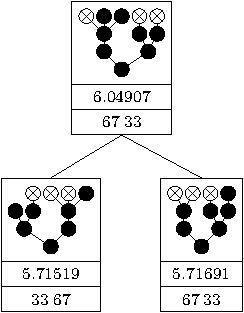
\includegraphics{p3/preemtive/0012233345_preemtive.pdf}
    \caption{A better preemtive schedule.}
  \end{subfigure}
  \caption{Preemtive vs. non-preemtive scheduling for $(0,0,1,1,1,2,2,2)$. Note that the snapshots in the second line are the same, but they are reached with different probabilities due to the fact that we can reschedule in the preemtive case.}
  \label{fig:preemtive-example-00111222}
\end{figure}

Another example that shows nicely that preemtive scheduling yields better results in some cases is the intree $(0,0,1,2,2,3,3,6,8,9,10,11,12,13)$ shown in figure \ref{fig:2-hlf-plus-one-not-optimal}. It is clear that -- if the first 6 steps, always the topmost task is the first task to finish, we at some point reach the intree shown in figure \ref{fig:preemtive-better-bad-case}. If we allowed to reschedule (by possibly interrupting the execution of some tasks) and chose a schedule as shown in figure \ref{fig:preemtive-better-good-case}, we would obviously acchieve a better overal run time. 

\begin{figure}[ht]
  \centering
  \begin{subfigure}{.46\textwidth}
    \centering
    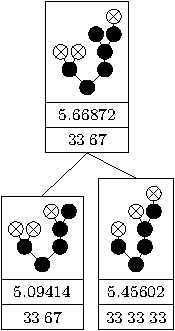
\includegraphics{p3/preemtive/00112556subopt.pdf}
    \caption{Suboptimal schedule. These snapshots are part of the optimal schedule for the intree $(0,0,0,2,3,4,5,7,7,9,10,10,12)$, shown in figure \ref{fig:2-hlf-plus-one-not-optimal}.}
    \label{fig:preemtive-better-bad-case}
  \end{subfigure}
  \quad
  \begin{subfigure}{.46\textwidth}
    \centering
    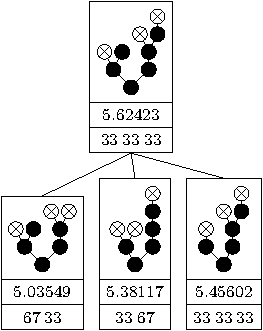
\includegraphics{p3/preemtive/00112556opt.pdf}
    \caption{Optimal schedule for $(0,0,1,1,2,5,5,6)$. This schedule is HLF.}
    \label{fig:preemtive-better-good-case}
  \end{subfigure}
  \caption{Intree $(0,0,1,1,2,5,5,6)$. This intree might result at some point from the intree $(0,0,1,2,2,3,3,6,8,9,10,11,12,13)$ with the two lowest tasks scheduled (see figure \ref{fig:2-hlf-plus-one-not-optimal}). If we allowed for preemting tasks we could improve the overal run time.}
  \label{fig:preemtive-is-better}
\end{figure}

\subsection{Considerations about subtrees}
\label{sec:properties-optimal-schedules-no-implications}

From another point of view, the intree $(0,0,1,2,2,3,3,6,8,9,10,11,12,13)$ shows that an optimal schedule may be forced at some time to process a subtree in a way that it would not process it if the subtree was processed for itself. This means that we can formulate the following:

\begin{theorem}
  There are intrees $T$ and $S$ such that $T$ is a subtree of $S$ and both $T$ and $S$ have the same root such that the optimal (non-preemtive) schedule for $S$ is HLF, but the optimal (non-preemtive) schedule for $T$ is non-HLF.
\end{theorem}

\begin{proof}
  See considerations above.
\end{proof}

\section{Size of the snapshot DAG}
\label{sec:p3-size-of-snapshot-dag-first-attempts}

Similar to the reasoning in section \ref{sec:p2-snapshot-dag}, we can research the size of a snapshot DAG for the P3 case. 
We conducted an experiment and examined the size for snapshot DAGs of intrees containing up to 17 tasks. 
Therefore, we generated all intrees (up to isomorphism) with a certain number of tasks (see section \ref{sec:enumerating-all-intrees} for an algorithm).
Then we computed the following for each intree:
\begin{itemize}
\item Number of distinct (i.e. non-isomorphic) subtrees.
\item Number of snapshots that can be constructed using the LEAF scheduling strategy (i.e. ``try-everything'' scheduling).
\item The size of the \emph{optimal} snapshot DAG.
\end{itemize}

We do so because of the following: It is easily possible to construct an optimal schedule if we take the possible snapshot DAGs of the LEAF scheduler and only leave the choices that yield the best expected run time.

Since the size of the snapshot DAG for an intree with $n$ tasks is at most $n^3$ times as large as the number of subtrees of the original intree, we also computed the number of subtrees for each of these intrees.
That is, we can compare the number of intrees to the number of snapshots to be considered.

The results are summed up in table \ref{tab:num-subtrees-size-of-dags}\todo{Complete!}.

\begin{table}[ht]
  \centering
  \begin{tabular}[ht]{ccccccc}
    \multirow{2}{*}{Tasks} & \multicolumn{2}{c}{Subtrees} & \multicolumn{2}{c}{Snapshots} & \multicolumn{2}{c}{``Optimal DAG''} \\
    & Max & Avg & Max & Avg & Max & Avg \\
    \hline
    3 & 3 & 3.00 & 3 & 3.00 & 3 & 3.00  \\
    4 & 5 & 4.25 & 5 & 4.25 & 5 & 4.25  \\
    5 & 7 & 5.89 & 7 & 5.89 & 7 & 5.89  \\
    6 & 11 & 8.10 & 11 & 8.25 & 11 & 8.05  \\
    7 & 16 & 11.04 & 19 & 11.75 & 16 & 10.81  \\
    8 & 24 &  15.10 & 34 & 17.39 & 22 & 14.37  \\
    9 & 34 &  20.57 & 63 & 26.53 & 31 & 18.76  \\
    10 & 54 &  28.08 & 119 & 41.85 & 41 & 24.16  \\
    11 & 79 &  38.33 & 230 & 67.48 & 55 & 30.67  \\
    12 & 119 & 52.41 & 437 & 112.68 & 71 & 38.41  \\
    13 & 169 &  71.69 & 812 & 184.95 & 89 & 47.49  \\
    14 & 269 &  98.19 & 1510 & 304.41 & 113 & 58.05  \\
    % 15 & 357 &  125.70 & 142 & 67.83  \\
    % 16 & 594 &  171.29 & 184 & 80.55  \\
    % 17 & 850 &  240.39 & 235 & 96.67  \\
  \end{tabular}
  \caption{Number of subtrees, size of the optimized snapshot DAG depending on the number of tasks. ``Subtrees'' denotes the number of distinct subtrees. ``Snapshots'' shows the number of distinct snapshots that have to be examined if we try all possible schedules. The column ``Optimal DAG'' shows the size of the snapshot DAG describing the optimal schedule.}
  \label{tab:num-subtrees-size-of-dags}
\end{table}

As we can see in table \ref{tab:num-subtrees-size-of-dags}, the number of subtrees is (at least for $n\geq  9$) significantly larger than the number of snapshots in the snapshot DAG describing an optimal schedule.

Another interesting fact is that there is no ``strict correlation'' between the number of subtrees and the number of snapshots in the optimal snapshot DAG. That is, there are certain DAGs that have more non-isomorphic subtrees than another DAG, yet -- on the other hand -- more snapshots in the optimal snapshot DAG. As an example, consider the intrees $T_1$ described by 00011111 and $T_2$ described by 00001234: $T_1$ has 19 subtrees and its optimal snapshot DAG contains 13 snapshots, while $T_2$ has only 15 subtrees, but an optimal snapshot DAG containing 14 snapshots.

Moreover, intrees containing $n$ tasks and having the maximal number of subtrees are (at least for $8\leq n \leq 17$) are not the ones having the largest optimal snapshot DAG.

To determine the maximum size of the optimal snapshot DAG for the P3 case, it might be useful to investigate whether the trees that have a large snapshot DAG can be constructed according to a specific pattern. The intrees resulting in snapshot DAGs of maximum size are depicted in figure \ref{fig:intrees-maximum-snapshot-dag-size-p3}. The intrees in this figure seem to behave quite chaotic and we were not able to deduce any pattern according to which they could be generated for general $n$.

\begin{figure}[t]
  \centering
  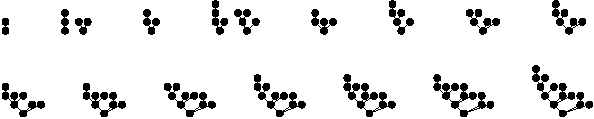
\includegraphics[scale=1.4]{p3/max_unoptimized.pdf}
  \caption{These are the intrees for which the a brute-force algorithm has to generate maximally many snapshots to generate the optimal schedule (maximal compared to all other intrees with the same number $n$ of vertices). We show $2\leq n \leq 14$.}
  \label{fig:intrees-maximum-unoptimized-p3}
\end{figure}

\begin{figure}[t]
  \centering
  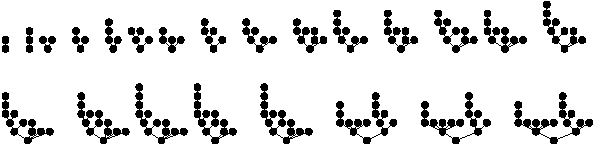
\includegraphics[scale=1.4]{p3/max_snapshot_dag.pdf}
  \caption{These intrees result in \emph{optimal} snapshot DAGs that are larger than all other optimal snapshot DAGs resulting from intrees having the same number of tasks $n$ ($2 \leq n \leq 17$ shown). There seems to be no simple pattern according to which these trees are constructed.}
  \label{fig:intrees-maximum-snapshot-dag-size-p3}
\end{figure}

% \section{Special classes of intrees}
% \label{sec:p3-dag-size-special-class-of-intrees}

% If we consider trees. whose sequence description is of the form $(0, 0, 1, 1, 3, 3, 5, 5, 7,7, 9,9,\dots)$, that have an even number of nodes, then the optimal snapshot DAGs have $\binom{n}{1}+\binom{n}{2}+\binom{n}{3}$ snapshots. \todo{Make this conjecture and nice!}

% \begin{table}[ht]
%   \centering
%   \begin{tabular}{lcc}
%     Class & No. snaps & Opt. size \\
%     $(0,0,1,1,3,3,5,5,\dots)$ & & $\binom{n/2}{1}+\binom{n/2}{2}+\binom{n/2}{3}$ \\
%     $(0,0,0,1,1,1,4,4,4,7,7,7,\dots)$ & & $((n/3)^3 + 2*(n/3))/3$
%   \end{tabular}
%   \caption{Classes and their DAG sizes}
%   \label{tab:special-classes-dag-sizes}
% \end{table}

\section{Degenerate intrees}
\label{sec:p3-degenerate-intrees}

\todo{Definitions: intree, level, suc, adding tasks to trees etc.}

We now focus one one particular class on intrees, namely \emph{degenerate intrees}. A degenerate intree is an intree that consists of one longest chain from the bottom to one leaf, and all other tasks are direct predecessors to one of the tasks within this longest chain. Another characterization is the following: On each level, \emph{at most one task} has predecessors.\todo{Figure zeigen.}

\subsection{Intro: Degenerate binary trees}
\label{sec:p3-degenerate-trees-binary}

We researched degenerate binary trees, i.e. trees whose sequence has the structure
\begin{equation*}
  \left( 0,0,a_0,a_1,a_2,a_3,a_4,\dots,a_n \right),
\end{equation*}
for $n+3$ the total number of tasks within the intree. The values $a_i$ can be recursively defined as follows:
\begin{equation*}
  a_k =
  \begin{cases}
    1, & \text{if } k\leq 1 \\
    a_{k-1}, & \text{if } k>1 \text{ is odd} \\
    a_{k-1}+2, & \text{if } k>1 \text{ is even}
  \end{cases}
\end{equation*}

That is, degenerate binary trees have sequences of the form $(0,0,1,1,3,3,5,5,7,7,9,\dots)$.

We now examine how many snapshots are considered if we compute the optimal P3 schedule by considering \emph{all} possibilities and afterwards discarding the bad ones. The results are summed up in table \ref{tab:p3-degenerate-binary-trees-no-snapshots}. We clearly observe that the number of snapshots grows exponentially (at least within the range for $n$ under consideration). A simple pattern that can be observed from table \ref{tab:p3-degenerate-binary-trees-no-snapshots} is that (at least for $n\leq 26$) that the number of snapshots for a degenerate binary tree with $n$ tasks is greater than twice the number of snapshots for a degenerate binary tree with $n-2$ tasks. If $S(n)$ denotes the number of snapshots for a degenerate binary tree, we can formulate $S(n)>S(n-2)$, which we can (by induction) convert to $S(n) > \sqrt 2 ^ n$.

This can be illustrated by the fact that degenerate binary intrees are fully determined by their profile (please see section \ref{sec:p2-profiles} for the definition of profiles). A degenerate binary tree has a profile of the form
\begin{equation*}
  \profile{a,2,2,2,2,\dots,2,1},
\end{equation*}
where $a$ is either $1$ or $2$. Assume the length of the profile (i.e. the height of the degenerate binary tree) is exactly $l$. Then, we have $2\cdot(l-2)+1+a = 2l-1+a$ tasks in total. Assume for now that $a=2$ (i.e. we are dealing with a complete degenerate binary tree) and $l>2$.

A subtree of a this degenerate binary intree having height $l'$ has a profile of the form
\begin{equation*}
  \profile{a_0,a_1,a_2,\dots,a_{l'-2},1},
\end{equation*}
where $1\leq a_0\leq a$ and $1\leq a_i \leq 2$ for all $i\in\left\{ 1,2,\dots,l-2 \right\}$. Using basic combinatorics, we can tell that there must be
\begin{equation*}
  \sum_{l'=0}^{l-1} 2^{l'} = 2^{l} -1
\end{equation*}
distinct subtrees if $a=2$ for profile length (resp. intree depth) $l$.

If $a=1$ and we have a profile length of $l$, we cann argue that there must be as many subtrees as for the profile without the first item (then of length $l-1$) plus the number of profiles of length exactly $l-1$ with one additional 1 prepended. These are exactly $2^{l-2}$.

This, in total leads to our desired bound for $S(n)$.\todo{Genauer machen.}

\begin{table}[t]
  \centering
  \begin{tabular}[ht]{ccc}
    \multirow{2}{*}{Tasks} & \multicolumn{2}{c}{Snapshots} \\
    & Overall & HLF \\
    \hline
    3  &  3       & 3   \\
    4  &  5       & 5   \\
    5  &  7       & 7   \\
    6  &  11      & 11  \\
    7  &  17      & 14  \\
    8  &  28      & 21  \\
    9  &  48      & 25  \\
    10 &  85      & 36  \\
  \end{tabular}
  \begin{tabular}[ht]{ccc}
    \multirow{2}{*}{Tasks} & \multicolumn{2}{c}{Snapshots} \\
    & Overall & HLF \\
    \hline
    11 &  150     & 41  \\
    12 &  276     & 57  \\
    13 &  477     & 63  \\
    14 &  884     & 85  \\
    15 &  1477    & 92  \\
    16 &  2717    & 121 \\
    17 &  4398    & 129 \\
    18 &  7991    & 166 \\
  \end{tabular}
  \begin{tabular}[ht]{ccc}
    \multirow{2}{*}{Tasks} & \multicolumn{2}{c}{Snapshots} \\
    & Overall & HLF \\
    \hline
    19 &  12600   & 175 \\
    20 &  22594   & 221 \\
    21 &  34883   & 231 \\
    22 &  61774   & 287 \\
    23 &  93775   & 298 \\
    24 &  164187  & 365 \\
    25 &  245852  & 377 \\
    26 &  426089  & 456 \\
  \end{tabular}
  \caption{Number of snapshots for degenerate binary trees in the P3 case. The first column shows the number of tasks. ``Overall'' denotes the number of distinct snapshots that are explored if an optimal schedule is constructed by examining all schedulings. ``HLF'' denotes the number of distinct snapshots for HLF.}
  \label{tab:p3-degenerate-binary-trees-no-snapshots}
\end{table}

Interestingly, degenerate binary intrees, while having a possibly huge amount of snapshots, are probably optimally scheduled by HLF. You can compare the number of HLF snapshots to the number of overal snapshots by looking at table \ref{tab:p3-degenerate-binary-trees-no-snapshots}.

We generalize this fact in the next section.

\subsection{HLF is optimal for degenerate intrees}
\label{sec:p3-degenerate-intrees-hlf-optimal}

\begin{lemma}
  \label{lem:p3-adding-tasks-level-keep-scheduled-same-inequality}
  Let $I$ be a degenerate intree and $x, y$ two (not necessarily distinct) ready tasks within this intree. Let $z_1, z_2$ be two new tasks that will be added to this intree with $level(z_1) > level(z_2)$ in a manner such that $I_1:=I\cup\left\{ z_1 \right\}$ and $I_2:=I\cup\left\{ z_2 \right\}$ are still degenerate intrees. Moreover, the tasks $z_1$ and $z_2$ shall be added in such a way that neither $x$ nor $y$ is a successor of $z_1$ or $z_2$ (i.e. $x,y$ stay ready in $I_1$ resp. $I_2$). 
  
  By $T^*_{t_1,t_2,t_3}(I)$ we denote the optimal expected run time that can be acchieved if we \emph{initially} schedule all tasks from the set $\left\{ t_1,t_2,t_3 \right\}$. \todo{Notation auslagern.} Note that this notation does not necessarily require that we actually have three tasks (e.g. if $t_1=t_2$).
  
  Then, if $x,y$ and $z_1$ resp. $z_2$ are used as initial tasks, we have the following for the best acchievable expected run times (for respective initial tasks):
  \begin{equation}
    \label{eq:lemma-p3-adding-tasks-level-keep-scheduled-same-inequality}
    T^{*}_{x,y,z_1}\left(I\cup\left\{ z_1 \right\}\right) > T^{*}_{x,y,z_2}\left( I\cup\left\{ z_2 \right\} \right)
  \end{equation}

  If we loosen the level condition to $level(z_1)\geq level(z_2)$, we obtain
  \begin{equation*}
    T^{*}_{x,y,z_1}\left(I\cup\left\{ z_1 \right\}\right) \geq T^{*}_{x,y,z_2}\left( I\cup\left\{ z_2 \right\} \right).
  \end{equation*}
\end{lemma}

\begin{proof}
  We focus first on the case where $level(z_1) > level(z_2)$ and prove the claim by induction over the number of nodes:
  
  The induction basis is the case where we have degenerate intrees with 3 tasks\footnote{We start by 3 tasks since these trees are the only ones that allow adding $z_1$ and $z_2$ at different levels such that both $x$ and $y$ stay ready. For an intree with two tasks, the claim can be seen by simply examining that $T(0,0)<T(0,1)$\todo{Improve this footnote.}.} (all of them are depicted in figure \ref{fig:p3-lemma-adding-intrees-induction-start} (only the black nodes)).
  
  \begin{figure}[t]
    \centering
    \begin{tikzpicture}[scale=0.25]
      \newcommand{\treeone}{
        \fill(0,0) circle (0.4);
        \fill(0,1) circle (0.4);
        \fill(0,2) circle (0.4);
        \draw(0,0) -- (0,1);
        \draw(0,1) -- (0,2);
      }
      \newcommand{\treetwo}{
        \fill(0,0) circle (0.4);
        \fill(-.50,1) circle (0.4);
        \fill(.50,1) circle (0.4);
        \draw(0,0) -- (0.5,1);
        \draw(0,0) -- (-.5,1);
      }
      \newcommand{\treethree}{
        \fill(0,0) circle (0.4);
        \fill(0,1) circle (0.4);
        \draw(0,0) -- (0,1);
      }
      % \begin{scope}
      %   \treeone;
      % \end{scope}
      % \begin{scope}[xshift=9cm]
      %   \treetwo;
      % \end{scope}

      \begin{scope}[yshift=-5cm, xshift=-20.5cm]
        \begin{scope}
          \treethree;
          \draw(0,1) -- (0,2);
          \draw[fill=white](0,2) circle (0.4);
          \node at (0,-2) {3};
        \end{scope}
        \node at (2.5,-2) {$>$};
        \begin{scope}[xshift=5cm]
          \treethree;
          \draw(0,0) -- (1,1);
          \draw[fill=white](1,1) circle (0.4);
          \node at (0,-2) {2.5};
        \end{scope}
      \end{scope}

      \begin{scope}[yshift=-5cm, xshift=-3.5cm]
        \begin{scope}
          \treeone;
          \draw(0,2) -- (0,3);
          \draw[fill=white](0,3) circle (0.4);
          \node at (0,-2) {4};
        \end{scope}
        \node at (2.5,-2) {$>$};
        \begin{scope}[xshift=5cm]
          \treeone;
          \draw(0,1) -- (1,2);
          \draw[fill=white](1,2) circle (0.4);
          \node at (0,-2) {3.5};
        \end{scope}
        \node at (8,-2) {$>$};
        \begin{scope}[xshift=11cm]
          \treeone;
          \draw(0,0) -- (1,1);
          \draw[fill=white](1,1) circle (0.4);
          \node at (0,-2) {3.25};
        \end{scope}
        % \node at (4,-1.5) {$4 > 3.5 > 3.25$};
      \end{scope}

      \begin{scope}[yshift=-5cm, xshift=20cm]
        \begin{scope}[xshift=0cm]
          \treetwo;
          \draw(-.5,1) -- (-.5,2);
          \draw[fill=white](-.5,2) circle (0.4);
          \node at (0,-2) {3.25};
        \end{scope}
        \node at (2.5,-2) {$>$};
        \begin{scope}[xshift=5cm]
          \treetwo;
          \draw(0,0) -- (1.5,1);
          \draw[fill=white](1.5,1) circle (0.4);
          \node at (0,-2) {2.83};
        \end{scope}
      \end{scope}
      
    \end{tikzpicture}
    \caption{Adding new tasks to degenerate intrees with less than four nodes such that the resulting intrees are still degenerate. The original (2- resp. 3-node) intrees are drawn black, the newly added tasks are drawn white. Below each intree, we see the corresponding optimal expected run time. The lower the level of the newly added task, the lower the expected run time. This serves as basis for the induction proof for lemma \ref{lem:p3-adding-tasks-level-keep-scheduled-same-inequality}.}
    \label{fig:p3-lemma-adding-intrees-induction-start}
  \end{figure}

  If we add two tasks $z_1$ and $z_2$ with $level(z_1)>level(z_2)$ in a way such that the original ready tasks stay ready and the resulting intrees stay degenerate, we obtain the intrees depicted in figure \ref{fig:p3-lemma-adding-intrees-induction-start} (trees \emph{including} the white nodes). By simply computing the expected optimal run times, we can confirm our claim for intrees with 3 nodes.

  We now do the induction step by considering an intree with $n$ tasks. 
  Let $x,y$ be ready tasks and $z_1$ and $z_2$ to be added with $level(z_1) > level(z_2)$ such that the resulting intrees are degenerate.
  We can now compare the two runs that can occur if $x,y,z_1$ resp. $x,y,z_2$ are initially scheduled. 
  Therefore, we consider what happens in $I_1=I\cup\left\{ z_1 \right\}$ resp. $I_2=I\cup\left\{ z_2 \right\}$ if either $x$, $y$ or $z_1/z_2$ finishes first:

  \begin{itemize}
  \item If $z_1$ resp. $z_2$ is the first task to finish, the resulting intree is exactly $I$. Thus, the remaining run times for these cases are identical if the next task chosen is the same in both trees. We denote the task that may be chosen additionally to $x$ and $y$ by $z'$. If it is the case that only $x$ and $y$ can be scheduled, we set $z'=x$ to simplify notation. The corresponding run time for the resulting intree is then $T^*_{x,y,z'}(I)$.

  \item If $x$ is the first task to finish, then the resulting intrees are 
    \begin{equation*}
      I^x_{1}=I_1\setminus\left\{ x \right\} \quad \text{ resp. } \quad I^x_{2}=I_2\setminus\left\{ x \right\}.
    \end{equation*}

    By $x'$ we denote the task that is scheduled next in the optimal schedule for intree $I_1^x$. 
    If there are only two ready tasks left in $I_1^x$ (which then must be $y$ and $z_1$), we set $x'=y$. The expected optimal runtime for $I_1^x$ in this situaion is then given by $T_{x',y,z_1}^*(I_1^x)$.

    We now examine whether $x'$ is also ready in the intree $I_2^x$:
    \begin{itemize}
    \item If there are only two ready tasks left in $I_1$ (namely $x$ and $y$), we set -- as mentioned before -- $x'=y$. Thus, in $I_2^x$, $x'$ is still ready\footnote{It may even be the case that $I_2^x$ contains some additional ready tasks that are not ready in $I_1^x$.}.
    \item If $x'$ is the direct successor of $x$, then $x$ must have been the \emph{single topmost task} and the \emph{single predecessor} of $x'$ (since $I_1^x$ is a degenerate tree). However, since we assumed that $level(z_2)<level(z_1)$ and $z_1$ can not be a predecessor of $x'$ (since $x'$ is ready in $I_1$), it can not be the case that $z_2$ blocks $x'$ in $I_2^x$. We conclude that in this case $x'$ is ready in $I_2^x$.

      % Moreover, since $x'$ is ready in $I_1^x$, the task $z_1$ can not be a predecessor of $x'$. Since $level(z_2)<level(z_1)$ and since $I_1^x$ and $I_2^x$ are both degenerate intrees, $z_2$ can not block $x'$.\todo{Genauer ausführen. Evtl. auslagern.}
    \item If $x'$ is not the direct successor of $x$, we recognize the fact that $x'$ must reside on a certain level with in the degenerate intree. 

      If $x'$ is \emph{not} in the topmost level, it can not be blocked by $z_2$ because we assumed that $z_2$ is added in a way such that $I\cup\{z_2\}$ is still a degenerate intree.

      Otherwise (if $x'$ is a topmost task), $z_2$ can not be added \emph{above} $x'$ because we assumed $level(z_1)>level(z_2)$.

      Again, $x'$ is ready in $I_2^x$.
      % we still have two subcases:
      % \begin{itemize}
      % \item If there are other tasks at the same level as $x'$ (i.e. at the topmost level), then we can -- without loss of generality\footnote{Because of isomorphism.} -- assume that $z_2$ was added to another task on the same level as $x'$.
      % \item If $x'$ was the \emph{only} topmost task, then it \emph{might} be the case that $z_2$ was chosen in a way such that it is the direct predecessor of $x'$. In this case, we can argue that $level(z_1) > level(z_2)$ and, thus, know that $z_2$ can not block $x'$, because $x'$ is a topmost task.
      % \end{itemize}

      % $x'$ must be on a lower level then $x$ (because we are dealing with a degenerate intree). We assumed that we added $z_2$ in a manner such that $I_2=I\cup\left\{ z_2 \right\}$ is a degenerate subtree. Thus, $z_2$ could not have been added with $x'$ as its successor. Thus, $x'$ is not blocked by $z_2$ in $I_2$.
    \end{itemize}
    We observed that for $I_2^x$, the task $x'$ must be ready.
    
    The intrees $I^x_{1}$ and $I^x_{2}$ have exactly $n$ tasks -- and they have a common subtree, namely
    \begin{equation*}
      I^x := I^x_{1}\setminus\left\{ z_1 \right\}=I^x_{2}\setminus\left\{ z_2 \right\}.
    \end{equation*}

    
    We can now apply the induction hypothesis for the intree $I^x$, since this intree contains only $n-1$ tasks: We have an intree with $n-1$ tasks (namely $I^x$) and two tasks $z_1$ and $z_2$ with $level(z_1)>level(z_2)$, $I^x_1 = I^x\cup\left\{ z_1 \right\}$ and $I^x_2 = I^x\cup\left\{ z_2 \right\}$, implying that $T^*_{x',y,z_1}(I^x_1)>T^*_{x',y,z_2}(I^x_{2})$.
  \item If $y$ is the first task to finish, we argue similar to the $x$ case, thereby considering $I^y_{1},I^y_{2}$ and $I^y$ which are all defined analogously. This finally yields the following inequality: $T^*_{x,y',z_1}(I^y_{1}) > T^*_{x,y',z_2}(I^y_{2})$.
  \end{itemize}

  The above considerations are illustrated in figure 
\ref{fig:p3-adding-tasks-level-keep-scheduled-same-inequality}.\todo{Figure anpassen!}
  
  \begin{figure}[t]
    \centering
    \newcommand{\drawx}{
      \node[draw=black,circle] at (.9,3) {$x$};
    }
    \newcommand{\drawxx}{
      \node[draw=black,circle] at (.7,2) {$x'$};
    }
    \newcommand{\drawy}{
      \node[draw=black,circle] at (-1.5,4) {$y$};
    }
    \newcommand{\drawyy}{
      \node[draw=black,circle] at (-1.5,3) {$y'$};
    }
    \newcommand{\rawtriangle}{
      \draw
      [dotted, very thick,
      %fill=white!90!black, 
      rounded corners]
      (0,0) -- (3,2) -- (3.5,8) -- (-3.5,8) -- (-3,2) -- cycle;
    }
    \newcommand{\treetriangle}{
      \rawtriangle;
      \drawx;
      \drawy;
    }
    \newcommand{\abstand}{7.5cm}
    \begin{tikzpicture}[scale=.4]
      \begin{scope}[xshift=-\abstand]
        \treetriangle
        \node[draw=black,circle] at (0,6.5) {$z_1$};
      \end{scope}
      \begin{scope}[xshift=\abstand]
        \treetriangle
        \node[draw=black,circle] at (1,5) {$z_2$};
      \end{scope}
      
      \begin{scope}[xshift=-2*\abstand, yshift=-9cm]
        \rawtriangle
        \node[draw=black,circle] at (0,6.5) {$z_1$};
        \drawxx;
        \drawy;
      \end{scope}

      \begin{scope}[xshift=-\abstand, yshift=-9cm]
        \rawtriangle
        \node[draw=black,circle] at (0,6.5) {$z_1$};
        \drawx;
        \drawyy;
      \end{scope}

      \begin{scope}[xshift=0, yshift=-9cm]
        \treetriangle
        \node[draw=black,circle] at (.3,5.5) {$z'$};
      \end{scope}
      
      \begin{scope}[xshift=\abstand, yshift=-9cm]
        \rawtriangle
        \node[draw=black,circle] at (1,5) {$z_2$};
        \drawxx;
        \drawy;
      \end{scope}

      \begin{scope}[xshift=2*\abstand, yshift=-9cm]
        \rawtriangle
        \node[draw=black,circle] at (1,5) {$z_2$};
        \drawx;
        \drawyy;
      \end{scope}
      
      \draw[thick,->](-\abstand,0) -- +(0,-.8);
      \draw[thick,->](-\abstand-2cm,1) -- +(-\abstand+4cm,-1.6);
      \draw[thick,->](-\abstand+2cm,1) -- +(\abstand-4cm,-1.6);

      \begin{scope}[xshift=2*\abstand]
        \draw[thick,->](-\abstand,0) -- +(0,-.8);
        \draw[thick,->](-\abstand-2cm,1) -- +(-\abstand+4cm,-1.6);
        \draw[thick,->](-\abstand+2cm,1) -- +(\abstand-4cm,-1.6);
      \end{scope}
      
      % legend      
      \draw[decoration=brace,decorate=true](-11,8.25) --node[above]{$I_1$} +(7,0);
      \draw[decoration=brace,decorate=true](  4,8.25) --node[above]{$I_2$} +(7,0);
      \draw[decoration={brace,mirror},decorate=true](  -18,-9.5) --node[below, yshift=-.2cm]{$I^x_{1}$} +(6,0);
      \draw[decoration={brace,mirror},decorate=true](-10.5,-9.5) --node[below, yshift=-.2cm]{$I^y_{1}$} +(6,0);
      \draw[decoration={brace,mirror},decorate=true](   -3,-9.5) --node[below, yshift=-.2cm]{$I$} +(6,0);
      \draw[decoration={brace,mirror},decorate=true](  4.5,-9.5) --node[below, yshift=-.2cm]{$I^x_{2}$} +(6,0);
      \draw[decoration={brace,mirror},decorate=true](   12,-9.5) --node[below, yshift=-.2cm]{$I^y_{2}$} +(6,0);
    \end{tikzpicture}

    \caption{Proof sketch for lemma \ref{lem:p3-adding-tasks-level-keep-scheduled-same-inequality}. By induction hypothesis, we have that $T^*_{x',y,z_1}(I^x_{1}) > T^*_{x',y,z_2}(I^x_{2})$ and $T^*_{x,y',z_1}(I^y_{1}) > T^*_{x,y',z_2}(I^y_{2})$, from which we deduce $T^*_{x,y,z_1}(I_1) > T^*_{x,y,z_2}(I_2)$. Note that $z_2$ can not block $x'$ or $y'$ since $z_1$ didn't block any of the two and we required that adding $z_1$ resp. $z_2$ still results a degenerate tree.}
    \label{fig:p3-adding-tasks-level-keep-scheduled-same-inequality}
  \end{figure}
  
  Now we argue that the run times for $I_1$ and $I_2$ can be computed as follows:
  \begin{align*}
    T^*_{x,y,z_1}(I_1) & = 
      \frac{1}{3} + 
      \frac{1}{3}\cdot \left( 
        T_{x,y,z'}^*(I) + 
        T^*_{x',y,z_1}(I^x_{1}) +
        T^*_{x,y',z_1}(I^y_{1}) 
      \right)
      \\
    T^*_{x,y,z_2}(I_2) & = 
      \frac{1}{3} + 
      \frac{1}{3}\cdot \left( 
        T_{x,y,z'}^*(I) + 
        T^*_{x',y,z_2}(I^x_{2}) +
        T^*_{x,y',z_2}(I^y_{2}) 
      \right)
  \end{align*}

  We will now use the aforementioned inequalities $T^*_{x',y,z_1}(I^x_{1}) > T^*_{x',y,z_2}(I^x_{2})$ and $T^*_{x,y',z_1}(I^y_{1}) > T^*_{x,y',z_2}(I^y_{2})$:
\begin{align*}
    T^*_{x,y,z_1}(I_1) & = 
      \frac{1}{3} + 
      \frac{1}{3}\cdot \left( 
        T_{x,y,z'}^*(I) + 
        T^*_{x',y,z_1}(I^x_{1}) +
        T^*_{x,y',z_1}(I^y_{1}) 
      \right)
      > 
      \\
      & >
      \frac{1}{3} + 
      \frac{1}{3}\cdot \left( 
        T_{x,y,z'}^*(I) + 
        T^*_{x',y,z_2}(I^x_{2}) +
        T^*_{x,y',z_2}(I^y_{2}) 
      \right) 
      = T^*_{x,y,z_2}(I_2).
  \end{align*}

  This proves our claim for $level(z_1) > level(z_2)$. It is simple to obtain the claim for the version where $level(z_1) \geq level(z_2)$: If the levels are the same, the resulting degenerate intrees $I_1$ and $I_2$ are isomorphic (and there is an isomorphism that maps $z_1$ onto $z_2$), thus the optimal run time is the same. If the levels are different, we argument as in the beginning of the proof.
\end{proof}

\paragraph{Application of lemma \ref{lem:p3-adding-tasks-level-keep-scheduled-same-inequality}}

We presented lemma \ref{lem:p3-adding-tasks-level-keep-scheduled-same-inequality} in a way that involved adding tasks to a certain intree, because this related well to our proof technique. In practice, we can use it to compare two degenerate intrees with $n$ nodes and that have a common subtree containing $n-1$ nodes.

We can now derive the following theorem.

\begin{theorem}
  Degenerate intrees are optimally scheduled by HLF.
\end{theorem}

\begin{proof}
  Consider a degenerate intree with $n=3$ tasks. It is trivially clear that for P3, a HLF schedule is optimal for this intree (see figure \ref{fig:p3-lemma-adding-intrees-induction-start} to see what these intrees look like -- we simply can conclude examine all possible schedules and see that the optimal ones is exactly HLF).
  
  Consider now a degenerate tree $I$ with $n$ nodes and assume that we know that for all degenerate trees with $n-1$ nodes HLF is optimal for three processors. If $I$ has two or less topmost tasks, it is obvious that we have to use HLF (since we can use at most two processors and HLF is known to be optimal for two processors --- see chapter \ref{chap:p2}).

  Thus, we only have to focus on the case where $I$ has at least three ready tasks.

  If we choose three topmost tasks $x,y,z$ of $I$, we can argue as follows: If $x$ is the task that finishes first, for the resulting subtree $I\setminus \left\{ x \right\}$, we can be sure that we can choose the next task such that we adhere to HLF, thus choosing the optimal solution for $I\setminus\left\{ x \right\}$ (by induction hypothesis). The same holds if $y$ or $z$ finishes first.
  
  We now consider a (possibly) non-HLF schedule for $I$ and compare it to the HLF schedule described before.
  Let $x',y',z'$ be the tasks to be chosen such that at least $x\neq x'$ or $y\neq y'$ or $z\neq z'$. We can -- without loss of generality -- assume $level(x')\leq level(x)$, $level(y')\leq level(y')$, $level(z')\leq level(z)$. If $x'$ is the first task to finish, we consider the degenerate intree $I\setminus\left\{ x' \right\}$. Since $I \setminus \left\{ x' \right\}$ is a degenerate intree with $n-1$ tasks, it would be optimal to use HLF. However, using HLF may or may not be possible depending on our previous choices of $y'$ and $z'$. That is, the optimum for $I\setminus\left\{ x' \right\}$ \emph{might} be acchieved if we chose $y'$ and $z'$ accordingly. From this we can conclude that the optimal expected run time is at least $T_{HLF}\left( I\setminus\left\{ x' \right\} \right)$, where $T_{HLF}$ denotes the run time for HLF (which we know, by induction, is optimal).

  Now we compare the run time for $I\setminus\left\{ x' \right\}$ to the optimal run time for $I \setminus\left\{ x \right\}$, which is exactly given by $T_{HLF}\left( I \setminus\left\{ x \right\} \right)$. We recognize that $I\setminus\left\{ x' \right\}$ and $I\setminus\left\{ x \right\}$ have a common subtree, namely $I\setminus\left\{ x,x' \right\}$ with $n-2$ tasks.
  
  Moreover, we know that for both $I\setminus\left\{ x \right\}$ and $I\setminus\left\{ x' \right\}$ HLF is optimal (because of our induction hypothesis) and that for $I\setminus\left\{ x \right\}$ and $I\setminus\left\{ x' \right\}$ both $y$ and $z$ must be in the optimal (i.e. HLF) schedule since $y$ and $z$ are two of the three topmost tasks. At last, we have $level(x) \geq level(x')$.
  Thus, we can apply lemma \ref{lem:p3-adding-tasks-level-keep-scheduled-same-inequality} for the degenerate tree $I\setminus \{x,x'\}$ with tasks $y$ and $z$ and deduce that
  \begin{equation*}
    T_{x',y,z}(I\setminus\{x\}) 
    \leq 
    \underbrace{T_{x,y,z}(I\setminus\{x'\})}_{\text{Optimal for $I\setminus \{x'\}$}}.
  \end{equation*}
  Equality holds if $x$ and $x'$ are on the same level.

  As stated before, for the intree $I\setminus\{x'\}$, the schedule chosen \emph{might} be a non-HLF schedule. In this case, the schedule performs even worse than $T_{x,y,z}(I\setminus\{ x'  \})$, since the optimal schedule would choose $x,y,z$ as scheduled tasks. This means that
  \begin{equation*}
    T_{x,y,z}(I\setminus\{x'\})
    \leq
    T_{x'',y',z'}(I\setminus\{x'\}),
  \end{equation*}
  where $x''$ is the task chosen by the non-HLF schedule, finally implying (by $T_{HLF}(I\setminus\{x\}) \leq T_{x',y,z}\left( I\setminus\left\{ x \right\} \right)$) that
  \begin{equation*}
    T_{HLF}(I\setminus\{x\})
    \leq
    T_{x'',y',z'}(I\setminus\{x'\}).
  \end{equation*}
  %because the HLF schedule is at least as good as the schedule that starts out with tasks $x',y,z$.
  We argue similar for tasks $y$ and $y'$ resp. $z$ and $z'$ and finally obtain the following:

  \begin{eqnarray*}
    T_{x',y,z}(I\setminus\{x\})
    & \leq &
    T_{x'',y',z'}(I\setminus\{x'\}) \\
    T_{x,y',z}(I\setminus\{y\})
    & \leq &
    T_{x',y'',z'}(I\setminus\{y'\}) \\
    T_{x,y,z'}(I\setminus\{z\})
    & \leq &
    T_{x',y',z''}(I\setminus\{z'\}) \\
  \end{eqnarray*}
  Note that if e.g. $x=x'$, the above three equations are still satisfied.
  Combining the above inequalities yields that
  \begin{eqnarray*}
    %T_{HLF}(I) = 
    T_{x,y,z}(I) 
    & \leq & 
    \frac{1}{3} + \frac{1}{3} \cdot 
    \left( 
      T_{x',y,z}(I\setminus\{x\}) +
      T_{x,y',z}(I\setminus\{y\}) +
      T_{x,y,z'}(I\setminus\{z\})
    \right) 
    \leq \\
    & \leq &
    \frac{1}{3} + \frac{1}{3} \cdot 
    \left( 
      T_{x'',y',z'}(I\setminus\{x'\}) +
      T_{x',y'',z'}(I\setminus\{y'\}) +
      T_{x',y',z''}(I\setminus\{z'\})
    \right) \leq \\
    & \leq &
    T_{x',y',z'}(I)
  \end{eqnarray*}

  This finally shows that a HLF schedule is at least as good as an arbitrary other task, meaning that HLF is optimal for three processors on degenerate trees.
\end{proof}

\section{Parallel chains}
\label{sec:p3-parallel-chains}

We will now consider another class of intrees that can be shown to have HLF as optimal schedules.

\begin{definition}[Parallel chain]
  Let $I$ be an intree. We call $I$ a \emph{parallel chain}, if each task except the root has at most one predecessor. The root may have arbitrarily many predecessors.
\end{definition}

\todo{Figure von einer parallel chain.}

We start out by a lemma that we will use later. This lemma is an analogue variant of a lemma described in \cite{chandyreynoldsshortpaper1975}. While their lemma works for two processors and general intrees, our variant is for three processors, but restricted to parallel chains.

\begin{lemma}
  \label{lemma:parallel-chains-flatness}
  Let $I$ be an intree and $x$ and $y$ two ready tasks with $level(x) > level(y)$. Then, $T_{HLF}(I\setminus\{ x \}) < T_{HLF}(I\setminus\{ y \})$, where $T_{HLF}(I)$ denotes the run time that is acchieved if intree $I$ is scheduled according to HLF.
\end{lemma}

\begin{proof}
  \newcommand{\iminus}[1]{I\setminus\{#1\}}

  \todo{Induktionsanfang}

  We consider the HLF schedules on the intrees $I\setminus \{x\}$ and $I \setminus \{y\}$, with variable names as aforementioned. Note that the intrees $I\setminus \{x\}$ and $\setminus \{y\}$ have at least two common HLF-tasks (i.e. tasks that are scheduled by HLF). We call these two tasks $x_1$ and $x_2$. \todo{Erklären, was passiert, wenn es im nächsten Schritt nicht mehr drei, sondern weniger Tasks zur Verfügung gibt.}For the intree $\iminus{x}$, we call the third HLF-task $x_3$ and can compute its expected run time (for HLF) by
  \begin{equation*}
    T_{HLF}(\iminus{x}) = 
    \frac{1}{3} \cdot T(\iminus{x, x_1}) +
    \frac{1}{3} \cdot T(\iminus{x, x_2}) +
    \frac{1}{3} \cdot T(\iminus{x, x_3})
    .
  \end{equation*}
  On the other hand, for the intree $\iminus{y}$, we call the third HLF-task $x'$ and can compute its expected run time analogously by
  \begin{equation*}
    T_{HLF}(\iminus{y}) = 
    \frac{1}{3} \cdot T(\iminus{y, x_1}) +
    \frac{1}{3} \cdot T(\iminus{y, x_2}) +
    \frac{1}{3} \cdot T(\iminus{y, x'})
    .
  \end{equation*}
  We can now compare $T(\iminus{x, x_1})$ with $T(\iminus{y, x_1})$, $T(\iminus{x, x_2})$ with $T(\iminus{x, x_2})$ and $T(\iminus{x, x_3})$ with $T(\iminus{y, x'})$.
  
  The intrees $\iminus{x,x_1}$ and $\iminus{y,x_1}$ have a common subtree, namely $\iminus{x_1}$. By induction ($\iminus{x_1}$ has $n-1$ tasks, $level(x) > level(y)$), we know that the expected HLF run time for $\iminus{x,x_1}$ is less than the expected run time for $\iminus{y,x_1}$. Note that $\iminus{x, x_1}$ has at least as many ready tasks as $\iminus{y,x_1}$. So, if $\iminus{y,x_1}$ has two or less ready tasks, the claim is true, because it has been shown for two processors in \cite{chandyreynoldsshortpaper1975} and we -- moreover -- can use a third processor for$\iminus{x,x_1}$. This consideration can be done for $x_2$ in the same manner. 

  It remains to compare $T(\iminus{x, x_3})$ and $T(\iminus{y, x'})$. If $\iminus{y,x'}$ has fewer ready tasks than $T(\iminus{x, x_3})$, then we trivially have $T(\iminus{x, x_3}) \leq T(\iminus{y, x'})$ (similar to the case before, it has been shown for two processors, and we additionally can use a third processor for $\iminus{x,x_3}$). We, thus, focus on other cases.

  \begin{itemize}
  \item  If $level(x')=level(x_3)$, the intrees $\iminus{x'}$ and $\iminus{x_3}$ are isomorphic (we are dealing with parallel chains only), and can -- thus -- be considered equal in our computations. That is, we can w.l.o.g. assume $x'=x_3$ if the levels of $x'$ and $x_3$ are equal. In this case, we have that $T(\iminus{x, x_3})$ and $T(\iminus{y, x'})$ share a common supertree (namely $\iminus{x_3}=\iminus{x'}$), and we know -- by induction since $level(x)>level(y)$ that $T(\iminus{x, x_3}) < T(\iminus{y, x'})$.
  \item   If $level(x') \neq level(x_3)$, we know that $x_3$ is \emph{not} a HLF task in $\iminus{y}$, but $x'$ is. This means that $x'$ can only be a HLF task since it is not part of $\iminus{y}$. Therefore, we conclude that $y$ must be the same as $x_3$ (implying w.l.o.g. $\iminus{x,y}=\iminus{y,x'}$). This means that $level(x)>level(y)=level(x_3)$. Moreover, because $x'$ is only a HLF task because $x_3$ is not existent in $\iminus{y}$, we know that $level(x') < level(x_3)$. Combining the inequalities yields $level(x)>level(x')$. We can now argue that $\iminus{y}$ is (w.l.o.g.) a common supertree of $\iminus{x,y}=\iminus{x,x_3}$ and $\iminus{y,x'}$ with $n-1$ tasks. Since -- as explained before -- $level(x) > level(x_3)$, we can apply the induction hypothesis and conclude that $T(\iminus{x, x_3}) \leq T(\iminus{y, x'})$.
  \end{itemize}

  We have now shown, that in any case the following hold:
  \begin{eqnarray*} 
    T(\iminus{x, x_1}) \leq T(\iminus{y, x_1}) \\
    T(\iminus{x, x_2}) \leq T(\iminus{x, x_2}) \\
    T(\iminus{x, x_3}) \leq T(\iminus{y, x'})
  \end{eqnarray*}
  These inequalities can be used to derive the desired inequality.
\end{proof}

We now use lemma \ref{lemma:parallel-chains-flatness} to derive the following theorem.

\begin{theorem}
  Parallel chains are optimally scheduled by HLF.
\end{theorem}

\begin{proof}
  \newcommand{\iminus}[1]{I\setminus\{#1\}}
  \todo{Induktionsanfang.}
  We prove the claim by induction and can clearly observe that for any parallel chain with fewer than $5$ tasks, HLF is optimal. \todo{Figure mit allen parallel chains mit weniger als 5 tasks.}
  
  Consider the HLF run time for a parallel chain $I$ with $n$ tasks. Let $x_1,x_2,x_3$ denote the HLF tasks of $I$. We can compute the expected run time by
  \begin{equation*}
    T_{HLF}(I) = 
    \frac{1}{3} \cdot T(\iminus{x_1}) +
    \frac{1}{3} \cdot T(\iminus{x_2}) +
    \frac{1}{3} \cdot T(\iminus{x_3})
    .
  \end{equation*}
  For the parallel chains $\iminus{x_1}, \iminus{x_2}$ and $\iminus{x_3}$ (each having $n-1$ tasks) we know by induction that they are optimally scheduled by HLF. Note that -- if we start in an HLF manner -- we can choose the next tasks in a way such that for each of these intrees we behave according to HLF (because $x_1, x_2$ and $x_3$ are HLF tasks of $I$). This means, we can acchieve optimal run times for each of the three intrees.

  Now consider any other initial choice of tasks $y_1,y_2,y_3$. We can (w.l.o.g.) assume that $level(y_i)\leq level(x_i)$ for $i=1,2,3$ and we can assume (w.l.o.g.) $level(y_1) < level(x_1)$. The optimal expected run time for this initial choice of tasks is given by
  \begin{equation*}
    T_{\{y_1,y_2,y_3\}}(I) = 
    \frac{1}{3} \cdot T_{\{y_2,y_3,z_1\}}(\iminus{y_1}) +
    \frac{1}{3} \cdot T_{\{y_1,y_3,z_2\}}(\iminus{y_2}) +
    \frac{1}{3} \cdot T_{\{y_1,y_2,z_3\}}(\iminus{y_3})
    ,
  \end{equation*}
  where $z_i$ denotes the optimal task to be chosen if $y_i$ is the first task to finish and the expected run times noted above are the optimal ones that can be acchieved. We set $z_i$ to $y_{i+1(\mod 3)}$ if there are only two ready tasks in a subtree.
  
  We now apply lemma \ref{lemma:parallel-chains-flatness}: The parallel chains $\iminus{y_1}$ and $\iminus{x_1}$ share $I$ as common supertree and $level(x_1) > level(y_1)$. Applying the lemma shows that $T_{HLF}(\iminus{y_1}) > T_{HLF}(\iminus{x_1})$. We know by induction that $\iminus{y_1}$ is optimally scheduled by HLF, implying that $T_{y_2,y_3,z_1}(\iminus{y_1}) \geq T_{HLF}(\iminus{y_1})$. Combining the two inequalities gives $T_{y_2,y_3,z_1}(\iminus{y_1}) > t_{HLF}(\iminus{x_1})$.

  Similar to the proof of lemma \ref{lemma:parallel-chains-flatness}, we can argue that the parallel chain $\iminus{x_1}$ has at least as many ready task as $\iminus{y_1}$ and, thus, that $\iminus{x_1}$ has a lower expected HLF run time than $\iminus{y_1}$.

  The arguments work similar for $x_2$ resp. $x_3$ with $y_2$ resp. $y_3$ (where we can even allow the run times to be equal), resulting in our claim.

\end{proof}

%%% Local Variables:
%%% TeX-master: "../thesis.tex"
%%% End: 

%\chapter{First thoughts on implementation}
\label{chap:first-thoughts-on-implementation}

\section{Configuration DAG}
\label{sec:configuration-dag}

Initially we are dealing with an intree (i.e. each node has at most one successor) of tasks that have to be processed by a certain number of processors.

We will call the set of \emph{all} tasks $\alltasks$. If task $t_2$ can only be executed if $t_1$ already has been processed, we write $t_1 \neededfor t_2$. Moreover, we introduce a shorthand notation that allows us to ``chain'' several of these symbols: If there exist tasks $s_1,\dots,s_m$ ($m\in\mathbb N$), we write $t_1 \neededfor* t_2$ if we have $t_1 \neededfor s_1$ and $s_1 \neededfor s_2, s_2 \neededfor s_3, \dots, s_{m-1} \neededfor s_m$ and $s_m \neededfor t_2$ or if $t_1\neededfor t_2$ or if $t_1=t_2$.

\begin{definition}
  Let $\alltasks$ be a set of tasks, and $T \subseteq \alltasks$. We call $T$ an intree (of tasks) if there is one designated task $t_0\in\alltasks$ such that the following two conditions hold:
  \begin{eqnarray*}
    \forall  t \in T. & \quad t \neededfor* t_0 \\
    \forall  t \in T. & \quad t\neededfor s \Rightarrow s\in T
  \end{eqnarray*}
\end{definition}

\begin{definition}
  Let $T$ be an intree of tasks. Let $M\subseteq\alltasks$ be a set of tasks such that the following two conditions hold:
  \begin{itemize}
  \item $\forall t\in M.\, t \in T$
  \item $\forall t\in M.\, \nexists u \in T.\, u\neededfor t $
  \end{itemize}
  We then call the tuple $\left( T, M \right)$ a \emph{configuration}.
\end{definition}

%%% Local Variables:
%%% TeX-master: "../thesis.tex"
%%% End: 

\appendix{}

%\include{counterexamples/counterexamples}

%\bibliographystyle{alphabetic}
\nocite{*}
\printbibliography[notkeyword=oeis,title={Bibliography}]
%\printbibliography[title={Number sequences},keyword=oeis]

\end{document}
